\part{急 性 中 毒}

\chapter{急性中毒诊治通则}

进入人体的化学物质达到中毒量产生组织和器官损伤引起的全身性疾病称为中毒(poisoning)。引起中毒的化学物质称毒物(poison)。根据接触毒物的毒性、剂量和时间,通常将中毒分为急性中毒和慢性中毒两类:急性中毒是大量毒物在较短时间内进入人体引起的疾病,发病急,症状严重,变化迅速,如不积极治疗,可危及生命;慢性中毒是由长时间小量毒物进入人体蓄积引起,起病缓慢,病程较长,缺乏特异性中毒诊断指标,容易误诊和漏诊。本章主要阐述急性中毒。

急性中毒是威胁生命的疾病,急性中毒的早发现、早诊断、早处理对预后事关重大。掌握好急性中毒的诊断与救治原则是有效救治急性中毒的基础。应熟悉急性中毒处理程序,使急性中毒救治快捷有序有效。

\subsection{毒物的吸收、代谢与中毒机制}

\subsubsection{毒物吸收}

\paragraph{呼吸道}

主要形态是粉尘、烟雾、蒸气、气体毒物。毒物由肺部吸收的速度比胃黏膜快20倍。

\paragraph{消化道}

主要是生活性中毒吸收,吸收部位在胃与肠道,以小肠为主。胃内pH、胃肠蠕动及胃肠道内容物对吸收有影响。

\paragraph{皮肤黏膜吸收}

主要是脂溶性毒物如苯胺、有机磷农药,临床上尤应注意的是头皮、腋窝、腹股沟、四肢内侧等部位。

\subsubsection{毒物的代谢与排泄}

毒物吸收入机体代谢部位以肝肠为主,甚至为肾、胃肠、心、脑、脾、胰、肺、肾上腺、甲状腺、视网膜,各组织的网状内皮细胞也可进行代谢转化。

毒物的排泄以肾脏最为重要,其次胆道、肠黏膜、汗腺、肺、乳汁等。

从毒物在体内代谢、排泄过程,下列几点须重视:①消化道是生活性中毒吸收、排泄的主要器官,在急救中早期洗胃、导泻、利胆,可尽早减少毒物的吸收,加快毒物的排泄。②肾脏参与毒物在机体内代谢,同时又是毒物的主要排泄器官,因此保肾、利尿在抢救急性中毒中有重要意义。③肝脏是毒物在机体内代谢的重要器官,急性中毒患者观察肝脏功能,保护肝功能措施是不可忽视的。④呼吸道也是毒物的排泄器官,中毒时又易引起中毒性脑病和组织细胞缺氧,急救中保持呼吸道通畅,尽快有效给氧则有利于毒物的排出和保护组织细胞及大脑的功能。

\subsubsection{中毒机制}

毒物种类繁多,作用不一:①毒物对组织的直接化学刺激腐蚀作用:强酸、强碱可吸收组织中的水分,并与蛋白质或脂肪结合,使细胞变质、坏死。②缺氧:一氧化碳、硫化氢、氰化物等窒息性毒物通过不同途径阻碍氧的吸收、转运和利用。脑和心肌对缺氧敏感,易发生损害。③麻醉作用:有机溶剂和吸入性麻醉药有强亲脂性。脑组织和脑细胞膜类脂含量高,因而上述化学物可通过血脑屏障抑制脑功能。④抑制酶的活力:很多毒物是由其本身或其代谢产物抑制酶的活力而产生毒性作用,如有机磷农药抑制胆碱酯酶,氰化物抑制细胞色素氧化酶,重金属抑制巯基酶等。⑤干扰细胞膜或细胞器官的生理功能:如自由基能使肝细胞膜中脂肪酸发生氧化作用而导致线粒体、内质网变性,肝细胞坏死。酚类如五氯酚、二硝基酚等可使线粒体内氧化磷酸化作用释耦联,妨碍高能磷酸键的合成和贮存,结果释放大量能量而发热。⑥受体的竞争:如阿托品可竞争和阻断毒蕈碱受体,阿托品中毒出现胆碱能神经抑制现象。

\subsection{急性中毒的诊断思路}

正确的急性中毒临床诊治思路非常重要。诊断中应尽量避免误诊,如未能考虑患者接触毒药物的可能性而漏诊或误诊,昏迷、老年或婴幼儿患者不能提供详细而可靠的病史,容易出现这类问题;对于昏迷或意识状态改变患者,一定要将中毒作为可能原因之一,向患者、患者亲属、同事、医生等了解患者的现病史、既往史、用药史、生活习惯,生活环境,工作环境,性格变化,在生命体征稳定情况下进行仔细的体格检查,实验室常规检查,必要的毒药物检查,甚至CT、MRI检查等。临床上不乏有将毒药物引起意识状态改变误为精神心理性疾病或脑血管病;将一氧化碳中毒误为流感、食物中毒的病例;过于依靠实验室检查结果诊断或排除中毒,在有条件进行毒药物分析的医疗机构,许多医生对毒药物筛检往往有不正确的认识,误区一:只要送去一份血或尿的标本,就得到患者体内是否存在某种毒药物的答案;误区二:如果检验未能有阳性结果,就排除某种中毒的可能性,毒药物筛检试验所检测的内容是有限的几种,而且好的实验结果与标本种类(血、尿、胃内容)、标本收集时间、仪器的灵敏度和精确度、仪器检测的范围、检测方法的选择等有很大关系。外伤患者的中毒问题:创伤患者如交通肇事,家庭暴力或街头暴力受伤者中,有许多酒精中毒或药物滥用的基础上发生,工业生产中失火或居民区失火的伤者常有烧伤和毒物吸入中毒的同时发生,吸入的有毒物质包括一氧化碳、氰化物、有机磷、高铁血红蛋白形成物及其他有毒化学物质,这些毒物或者直接损伤呼吸系统,或者产生全身性中毒,由于外伤患者多具有明确的外伤史和明显可见的伤口,因此常常忽略了对同时存在的中毒的诊断和治疗,由此引起死亡率增高,并发症增多。医生遇到患者的全身状态与损伤程度不一致,或难以解释的意识改变,缺氧、发绀等体征或外伤得到很好控制,而意识或全身状态却不断恶化的情况,均应考虑有同时存在的中毒可能。又如急性有机磷农药中毒误诊为急性胃肠炎、支气管哮喘急性发作;毒鼠强中毒误诊为乙型脑炎,癫痫大发作;酒精中毒引发的并发症急性脑血管意外以为是酒精中毒的昏睡期等。

多数情况下,对患者进行仔细的检查和询问病史,可以得到重要线索,指导医生提出某些特定物质的检查,医生应该熟悉中毒时的一些特殊的症状和体征,通过体格检查,常规实验室检查,毒药物检查以及其他辅助检查的结果,动态观察病情变化,去伪存真地综合分析做出正确的诊断也不难。以下几点应加以注意:

1.细心询问病史、了解与中毒有关资料
①明确中毒时间,毒物种类,中毒途径,中毒量;②明确有关原发病史及中毒时前后情况;③明确中毒现场救治的相关资料。

2.认真分析中毒的临床表现
急性中毒可产生严重的症状,如发绀、昏迷、惊厥、呼吸困难、休克、尿闭等。

(1)
皮肤黏膜表现:①皮肤及口腔黏膜灼伤:见于强酸、强碱、甲醛、苯酚、来苏等腐蚀性毒物灼伤。硝酸可使皮肤黏膜痂皮呈黄色,盐酸痂皮呈灰棕色,硫酸痂皮呈黑色。②发绀:引起氧合血红蛋白不足的毒物可产生发绀。麻醉药、有机溶剂抑制呼吸中枢,刺激性气体引起肺水肿等都可产生发绀。亚硝酸盐和苯胺、硝基苯等中毒能产生高铁血红蛋白血症而出现发绀。③黄疸:四氯化碳、毒蕈、鱼胆中毒损伤肝脏可致黄疸。

(2)
眼部表现:①瞳孔扩大:见于阿托品、莨菪碱类中毒。②瞳孔缩小:见于有机磷农药、吗啡中毒。

(3)
神经系统表现:①昏迷:常见于麻醉药,催眠药、安定药等中毒;有机溶剂中毒、窒息性毒物中毒,如一氧化碳、氰化物等中毒;高铁血红蛋白生成性毒物中毒;农药中毒,如有机磷杀虫剂、有机汞杀虫剂,拟除虫菊脂杀虫剂、溴甲烷等中毒。②谵妄:见于阿托品、乙醇中毒。③肌纤维颤动:见于有机磷农药、氨基甲酸脂杀虫剂中毒。④惊厥:见于窒息性毒物中毒以及异烟肼、有机磷杀虫剂、拟除虫菊脂杀虫剂等中毒。⑤瘫痪:见于可溶性钡盐、箭毒、蛇毒等中毒。⑥精神失常:见于四乙基铅、二硫化碳、一氧化碳等中毒。

(4)
呼吸系统表现:①呼吸气味:有机溶剂挥发性强,而且有特殊气味,如酒味。氰化物有苦杏仁味;有机磷农药有大蒜味,苯酚、来苏有苯酚味。②呼吸加快:引起酸中毒的毒物如水杨酸、甲醇等可兴奋呼吸中枢,使呼吸加快。刺激性气体引起肺水肿时,呼吸加快。③呼吸减慢:见于催眠药、安定药、吗啡中毒,也见于中毒性脑水肿。呼吸中枢过度抑制可致呼吸麻痹。④肺水肿:刺激性气体、安妥、磷化锌、有机磷农药等中毒可引起肺水肿。

(5)
循环系统表现:心律失常:见于阿托品、拟肾上腺素药物、洋地黄、夹竹桃、蟾蜍等中毒。心脏骤停:可能由于:①毒物直接作用于心肌:见于洋地黄、奎尼丁、依米丁、河豚等中毒。②缺氧:见于窒息性毒物中毒。③低钾血症。休克:原因有:①剧烈的吐泻导致血容量减少。②严重的化学灼伤:由于血浆渗出而血容量减少。③毒物抑制血管舒缩中枢,引起周围血管扩张,有效循环血量减少。④心肌损害:如砷、锑、依米丁中毒等。

(6)
泌尿系统表现:急性肾功能衰竭:中毒后肾小管受损害,出现尿少以至无尿,常见于三种情况:①肾中毒伴肾小管坏死;如升汞、苯酚、磺胺、头孢菌素、蛇毒、毒蕈等中毒。②肾缺血。产生休克的毒素可致肾缺血。③肾小管堵塞:磺胺结晶可堵塞肾小管;毒物所致血管内溶血,游离血红蛋白由尿排出时可堵塞肾小管。

(7)
血液系统表现:①溶血性贫血:中毒后红细胞破坏增速,量多时发生贫血、黄疸。急性血管内溶血如砷化氢中毒,严重者可发生血红蛋白尿和急性肾功能衰竭。②白细胞减少:见于氯霉素、抗癌药等中毒。③出血:见于由阿司匹林、氯霉素、抗癌药等引起的血小板质或量异常,由蛇毒、杀鼠剂、肝素、水杨酸等引起的血液凝固障碍。

3.针对性体查 、明确与中毒相关体征
急性中毒的急救中,应采取边抢救边针对性体查。首先要明确患者的生命体征,是否有危及生命体征的险情,若有应先努力稳定生命体征,然后行严格系统查体:

(1)
皮肤黏膜与中毒相关的体征:①皮肤潮湿,提示中毒严重导致循环衰竭,大汗提示有机磷中毒。②皮肤黏膜发绀,提示亚硝酸盐中毒。③口唇黏膜樱红与皮肤潮湿,提示一氧化碳或氧化物中毒。④皮肤出血、瘀斑及肌肉颤动,提示敌鼠钠盐中毒。

(2)
呼吸功能与中毒相关的体征:①呼吸浅而慢,提示安眠药及一氧化碳中毒。②呼吸加快,提示有机磷农药中毒。③呼出气味似酒精味,提示酒精中毒。

(3)
心血管功能与中毒相关的体征:①血压降低,多与氯丙嗪类、安眠药中毒有关。因这类药物可使周围血管扩张,且能对抗肾上腺素中去甲肾上腺素的升压作用。②心动过速,多与阿托品类中毒有关。③心动过缓,多与洋地黄类制剂中毒有关。④心搏骤停,多与氰化物、硫化氢、有机磷农药中毒有关。

(4)
脑神经功能与中毒相关的体征:①躁动不安、幻听幻视,可能与阿托品类中毒有关。②四肢抽搐,可能与有机磷农药或异烟肼、杀鼠剂:如毒鼠强中毒有关。③低血钾性软瘫,可能与食用大量棉籽油(棉酚)中毒有关。④昏迷,提示中毒大量毒物,进入身体后导致患者昏迷。

(5)
胃肠功能与中毒相关的体征:①恶心、呕吐、腹痛、腹泻,提示中毒途径经消化道。②黄疸,提示毒物已导致肝功能受损。

(6)
肾功能衰竭与中毒:急性肾功能衰竭,提示与巴比妥类安眠药、鱼胆中毒有关。

(7)
血液系统功能与中毒相关的体征:①急性溶血,提示毒蕈类或砷化物、硫酸铜中毒有关。②出、凝血功能障碍,提示与蛇毒、灭鼠灵及敌鼠钠盐中毒有关。③白细胞总数下降,多与化学药物中毒有关。

(8)
瞳孔变化与中毒相关的体征:①瞳孔散大,提示阿托品类中毒有关。②瞳孔缩小,提示有机磷农药、安眠药中毒有关。

4.实验室检查
①毒物检验:采集剩余毒物、容器,可疑食物和水样,以及含毒物标本如呕吐物,第一次洗胃液、血、尿、便及其他可疑物品送检。②特异检验:如疑有机磷中毒查胆碱酯酶;一氧化碳中毒查碳氧化血红蛋白;亚硝酸盐中毒查高铁血红蛋白等。③动态监测病情变化:宜查血常规、血糖、血电解质、肝、肾功能、心电图、血压、血气分析、X线检查等。

5.预测病情危重指标
中毒可产生器官损害,引起多脏器功能失常和衰竭。若出现下列情况者,说明患者的中毒进入危重期,必须严密观察病情变化,积极维持机体器官的功能:①中枢神经系统抑制:出现昏迷、呼吸抑制、血压下降、惊厥、抽搐。②肺水肿。③严重的心律失常。④心脏骤停。⑤发绀。⑥急性溶血性贫血,血红蛋白尿。⑦急性肾衰竭、少尿、尿毒症。⑧肝性脑病。⑨烧伤、化学灼伤、眼灼伤。

6.鉴别诊断
急性中毒的鉴别诊断除了毒物中毒间的鉴别外,还须与下列疾病相鉴别:①脑血管意外,昏迷时多有偏瘫或脑膜刺激征和局灶定位体征。②心源性肺水肿,有心脏病史和相应的体征。③肺性脑病、发绀,有慢性肺病病史。④周期性瘫痪:血钾降低,补钾后症状改善快。⑤细菌性食物中毒(表\ref{tab53-1})。

\subsection{急性中毒的救治原则与措施}

\subsubsection{急性中毒救治原则}

急性中毒救治原则:①切断毒源:使中毒患者迅速脱离染毒环境。②迅速阻滞毒物的继续吸收:及早的洗胃、导泻、清洗皮肤和吸氧。③迅速有效消除威胁生命的毒效应:凡心搏和呼吸停止的应迅速施行心肺复苏术(CPR);对休克、严重心律失常、中毒性肺水肿、呼吸衰竭、中毒性脑病、脑水肿、脑疝应及时对症救治。④尽快明确毒物接触史:接触史包括毒物名称、理化性质与状态、接触时间和吸收量及方式,若不能立即明确,须及时留取洗胃液或呕吐物、排泄物及可疑染毒物送毒物检测。⑤尽早足量使用特效解毒剂。⑥当中毒的毒物不明者,以对症处理为先和早期器官支持为主。

\subsubsection{救治措施}

\hypertarget{text00130.htmlux5cux23CHP5-1-3-2-1}{}
(一) 清除尚未吸收的毒物

\paragraph{吸入性中毒}

应立即撤离中毒现场,保持呼吸道通畅,呼吸新鲜空气,吸氧。

\paragraph{接触中毒}

应立即脱去污染衣服,用清水洗净皮肤。注意冲洗皮肤不要用热水以免增加毒物的吸收;毒物如遇水能发生反应,应先用干布抹去沾染物,再用水冲洗。

\paragraph{经口中毒}

应采取催吐、洗胃、导泻法以排除尚未吸收毒物。洗胃是经口中毒清除未吸收毒物的主要方法,以下几点要特别注意:①洗胃以服毒6小时以内最有效。对服毒6小时以上也不应放弃洗胃。②洗胃的原则:早洗、反复洗、彻底洗。③洗胃液多以清水为宜,忌用热水。④每次灌入量以300~400ml(神志不清者减为100~300ml)为宜,直至洗出胃液清晰为止。一般成人洗胃液总量5000~10
000ml。⑤洗胃时应注意防止吸入性肺炎和水中毒,脑水肿。⑥对腐蚀性毒物(如强酸、强碱),挥发性烃类化学物(如汽油)口服中毒者宜禁忌洗胃。⑦对深昏迷、呼吸衰竭者,可先行气管内插管后,再下胃管洗胃。⑧洗胃管宜留置24小时间断洗胃,同时防止呕吐及洗胃液误入气管造成不良后果。洗胃过程应观察生命体征变化,及时处理威胁生命的症状。

\hypertarget{text00130.htmlux5cux23CHP5-1-3-2-2}{}
(二) 及时足量使用特效解毒剂

使用解毒剂的原则是:①早期、足量、尽快达到治疗有效量,注意防止副作用。②选择正确的给药方法,使特殊解毒剂在最短的时间内发挥最好的疗效。③注意解毒剂的配伍,充分发挥解毒剂的联合作用如对有机磷农药中毒-阿托品与胆碱脂酶复活剂的合用;毒鼠强中毒-地西泮与纳洛酮的合用等。特效解毒剂的具体用法参见有关章节。

\begin{table}[htbp]
\centering
\caption{细菌性食物中毒和化学性食物中毒的比较}
\label{tab53-1}
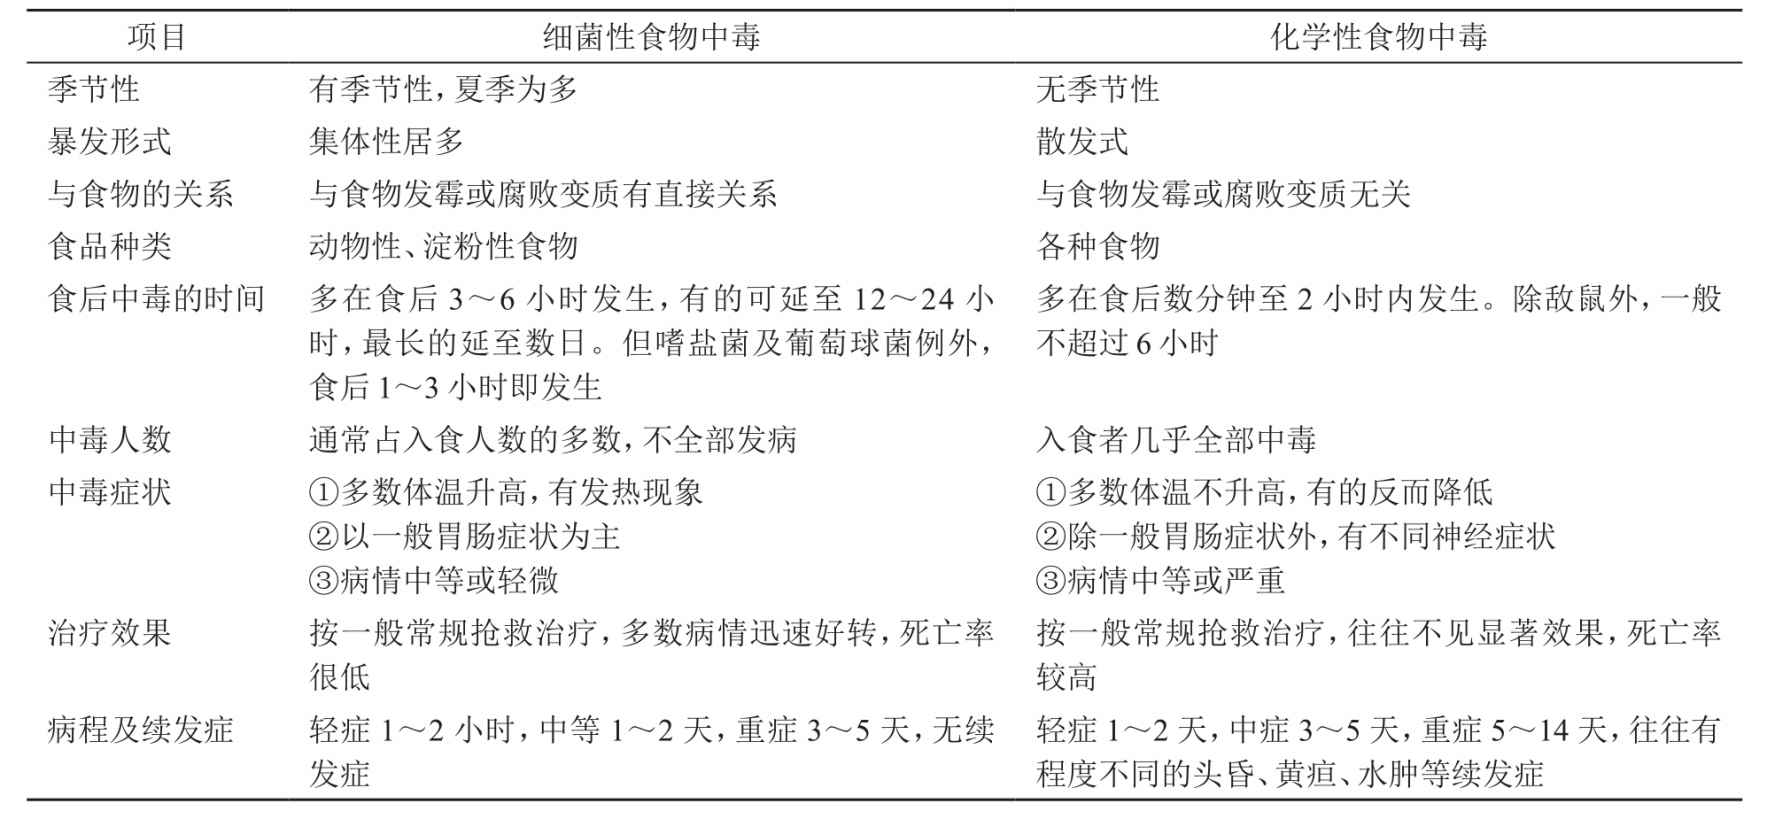
\includegraphics[width=6.64583in,height=3.07292in]{./images/Image00180.jpg}
\end{table}

\hypertarget{text00130.htmlux5cux23CHP5-1-3-2-3}{}
(三) 促进毒物的排泄

\paragraph{利尿排毒}

大多数毒物可由肾脏排泄,因此救治急性中毒注意保肾,有利于充分发挥迅速利尿来加速毒物排泄。①积极补液是促使毒物随尿排出的最简单措施。补液速度可每小时200~400ml。②碳酸氢钠与利尿剂合用;可碱化尿液(pH
8)使有些化合物(如巴比妥酸盐,水杨酸盐及异烟肼等)离子化而不易在肾小管内重吸收。③应用维生素C
8g/d,使尿液pH <
5,促使有些毒物(苯丙胺等)加速排出。④经补液与利尿剂后,水溶性的与蛋白结合很弱的化合物(如苯巴比妥、甲丙氨酯、苯丙胺及锂盐)较易从体内排出。

\paragraph{血液净化疗法}

是促进某些已吸收毒物的清除的主要措施。适应证有:①该毒物或其代谢产物能被透析清除出体外者;②估计中毒剂量大,预后严重者;③发生急性肾功能衰竭者。应争取在中毒后8~16小时内采用,疗效较佳。相对禁忌证有:①严重心功能不全者;②有严重贫血或出血者;③高血压患者收缩压>
220mmHg。目前常用的血液净化方法有以下几种:

\hypertarget{text00130.htmlux5cux23CHP5-1-3-2-3-2-1}{}
(1) 血液透析:

用透析器进行透析或超滤,适用于水溶性、不与蛋白或其他成分结合的分子量<
500的小分子和部分中分子毒物,如对乙酰氨基酚、水杨酸盐、非那西丁、苯巴比妥、甲丙氨酯(眠尔通)、水合氯醛、海洛因、甲醛、乙醇、乙二醇、溴剂、异丙醇、苯丙胺、锂盐、异烟肼、苯妥英钠、砷、铁、钾、钡、四氯化碳、硼酸盐等。脂溶性毒物的透析效果差,如格鲁米特(导眠能)等。与蛋白紧密结合的毒物,如短效作用的巴比妥盐类、吩噻嗪类药物、阿米替林等抗抑郁药及地西泮类药物等疗效也不佳。

\hypertarget{text00130.htmlux5cux23CHP5-1-3-2-3-2-2}{}
(2) 血液灌流:

是将血液在体外直接流经活性炭、树脂、氧化淀粉等吸附剂,将血液中的毒物吸附,以达到净化血液的目的。本法对去除脂溶性或与蛋白结合的毒物,效果较好。如镇静催眠药(巴比妥类、地西泮、导眠能、水合氯醛、甲丙氨酯、吩噻嗪类)、解热镇痛药(对乙酰氨基酚、水杨酸类)、三环类抗抑郁药(阿米替林、丙米嗪、多塞平)、抗癌药(甲氨蝶呤、5-Fu、6MP)、洋地黄类、异烟肼、苯丙胺、百草枯、毒鼠强、毒蕈毒素、有机磷农药、有机氯农药等。

\hypertarget{text00130.htmlux5cux23CHP5-1-3-2-3-2-3}{}
(3) 血浆置换:

适用于清除与血浆蛋白结合率高(>
60\%),不易被血液透析或灌流清除的毒物。但需要消耗大量血浆和血制品,并有传播病毒性疾病(肝炎病毒、艾滋病等)的危险,限制了它在中毒临床的应用。

\paragraph{换血疗法}

本法对各种毒物(硝酸盐、亚硝酸盐、氯化物、溴化物、磺胺、硝基苯、含氧化合物等)所致的高铁血红蛋白血症效果好。

\hypertarget{text00130.htmlux5cux23CHP5-1-3-2-4}{}
(四) 有效地对症处理

许多毒物至今尚无有效的解毒剂
,急救措施主要依靠及早排毒及有效的对症支持疗法。

\paragraph{氧疗法}

在急救中,氧疗是一种有效的治疗方法。急性中毒常因毒物的毒理作用而抑制呼吸及气体交换,有的毒物抑制组织内细胞呼吸造成组织缺氧。因此在救治中要监护呼吸,有效的吸氧疗法,正确选用鼻导管、面罩、呼吸机、高压氧给氧。

\paragraph{纠正低血压 、休克}

常见于镇静药、催吐药、抗精神病及抗抑郁药物中毒,其作用机制常是综合性的。除补充血容量外,要重视应用纳洛酮和血管活性药物的应用及中毒性心肌炎防治。

\paragraph{高热与低温的处理}

高热常见于酚噻嗪类、单胺氧化酶类及抗胆碱类等药物中毒,甚至可引起休克及恶性神经抑制综合征。低温多见于镇静安眠药物中毒,在低温可发生电解质、体液及酸碱失衡,细胞内钠丢失。故要及时处理。

\paragraph{心律失常}

有些毒物影响心肌纤维的电作用,另外由于心肌缺氧或代谢紊乱而发生心律失常。救治中早期应用镁极化液有助于预防心律失常,同时可根据心律失常的类型选择应用相应的药物,常用的有利多卡因、阿托品、维拉帕米、普罗帕酮、毛花苷丙,同时要关注电解质平衡。

\paragraph{心搏骤停}

除因严重缺氧外,也有某些毒物的直接作用引起阿-斯综合征所致,如急性有机磷农药或有机溶剂中毒,汽油、苯等刺激β受体,能突然导致原发性室颤而死亡,三氯甲烷、氟乙酸、氟乙酰胺等严重中毒时,可直接作用心肌发生心室颤动,引起心脏骤停,高浓度氯气吸入,可因迷走神经的反射增强而导致心脏骤停。一旦发生心脏骤停,应分秒必争紧急心肺、脑复苏,除有效的胸外心脏按压外,迅速开放气道,有效供氧十分重要,有条件时应尽快行气管内插管使用呼吸机。同时根据病情选用肾上腺素、阿托品、纳洛酮等。心肺复苏时间宜延长。

\paragraph{中毒性脑病}

主要由于亲神经毒物所致,如一氧化碳、二氧化碳、有机汞、麻醉药、镇静药。主要表现不同程度的意识障碍和颅内压增高症状。此外,抽搐、惊厥也是中毒性脑病的常见症状。中毒性脑病的救治重点是早发生、早防治脑水肿,保护脑细胞。根据病情适时应用脱水剂如20\%甘露醇125ml
+呋塞米20mg
+地塞米松10mg每3~12小时1次,出现抽搐、惊厥可用苯妥英钠,必要时用地西泮。常规使用ATP、辅酶A、胞二磷胆碱、吡拉西坦、纳洛酮等药物。

\paragraph{防治急性肾功能衰竭}

原则是有效控制原发病,维持有效血液循环,纠正缺氧,避免使用对肾有损害的药物,合理使用利尿剂。在利尿剂使用效果不佳时,注意选用血管扩张剂如酚妥拉明、阿托品、多巴胺等药物。

\hypertarget{text00130.htmlux5cux23CHP5-1-3-2-5}{}
(五) 注意内环境管理

急性中毒常因毒物本身的作用和患者呕吐
、腹泻、出汗、洗胃等均可造成内环境的紊乱,主要表现为电解质失衡,酸碱失常,如低血钾、低血钠、酸碱中毒等。在救治中主要注意监测电解质、酸碱平衡的状况。

\hypertarget{text00130.htmlux5cux23CHP5-1-3-2-6}{}
(六) 早期防治急性中毒致 MODS

早期识别MODS,早期防治,有利于降低急性中毒病死率。防治急性中毒致MODS的重点是:

\paragraph{早期识别急性中毒致 MODS}

急性重度中毒患者发病急、病情重,救治不及时可迅速发生MODS,甚至引起死亡,一旦出现,病死率达30\%~100\%。常见急性中毒致MODS的特点简述如下:

\hypertarget{text00130.htmlux5cux23CHP5-1-3-2-6-1-1}{}
(1) 急性有机磷农药中毒致MODS:

急性有机磷农药中毒(AOPP)可致MODS,引起心源性猝死、呼吸肌麻痹等并发症。①心脏的毒性损害:有机磷农药(OP)对心脏毒性损害的病理改变为心肌细胞脂肪变性,心肌间质充血、水肿、单核细胞浸润、心外膜点状出血、右心室和左心室轻度扩张,具有心肌纤维断裂现象。OP可引起各种类型的心律失常,机制可能与抑制胆碱酯酶(ChE)使神经末梢释放的乙酰胆碱(Ach)不能水解,从而影响心脏的传导功能。造成心源性猝死,可能是毒物造成的心肌麻痹或中毒性心肌炎。②呼吸系统损害:AOPP对呼吸系统的损害是最严重的。死亡的主要原因往往是呼吸衰竭。常见的原因有中毒性肺水肿、呼吸肌麻痹、呼吸中枢麻痹。③脑栓塞:OP是有强烈的神经毒样作用,可引起脑细胞间质水肿,细胞脂肪变性、脑屏障受损、脑组织毛细血管通透性增加以及阿托品的大量应用引起脑血管扩张均可导致脑水肿。脑损害的发生率占12\%。④中毒性肝损伤:OP在体内分布以肝脏浓度最高,其系非亲肝性毒物,但在较大剂量接触时,部分患者也可发生肝损害,尤以胃肠吸收者存在肝-肠循环,肝损害更为明显。氧自由基可能是肝细胞损伤的主要机制之一。OP在体内的代谢过程由肝脏完成,可产生大量氧自由基。谷丙转氨酶在中毒第2天达高峰并持续6天后逐渐下降。⑤中间综合征(IMS):IMS发生时间为OP中毒后2~4天,个别为7天,是AOPP经过救治后急性胆碱能危象(ACC)消失后,继发性周围神经病(OPIDP)之前出现的以肌无力为突出临床表现的一组综合征。有因呼吸肌麻痹致外周呼吸衰竭而死亡的危险。

\hypertarget{text00130.htmlux5cux23CHP5-1-3-2-6-1-2}{}
(2) 禁用杀鼠剂中毒致MODS:

禁用杀鼠剂是指20世纪80年代国家严禁使用的一类灭鼠剂如毒鼠强、氟乙酰胺、氟乙酸钠等,毒力极强,且都有明显的蓄积作用,人食用毒死的家畜可引起二次中毒。①脑功能障碍:毒鼠强进入人体后,拮抗中枢神经系统的γ-氨基丁酸(GABA)。尸检均有脑水肿和散在的脑组织死亡溶解。②心脏损害:是毒物直接损害心肌细胞造成心肌细胞损伤坏死,心肌酶谱异常增高。心电图可有ST段及T波改变。③肝功能障碍:毒物可直接作用肝细胞造成肝细胞损伤、坏死,引起肝脏转氨酶异常增高,且可出现黄疸。④肺水肿或ARDS,神经源性肺水肿。

\hypertarget{text00130.htmlux5cux23CHP5-1-3-2-6-1-3}{}
(3) 急性有害气体中毒致MODS:

常见的有害气体包括:一氧化碳、氰化物、硫化物、石油液化气、煤气等。国内宋国平报告重度一氧化碳中毒416例,发生MODS达76\%,治愈率93.3\%,死亡率1.2\%,以脑损害、心脏损害、肺损害为主,以昏迷、呼吸困难、心电图异常为主要表现。

\hypertarget{text00130.htmlux5cux23CHP5-1-3-2-6-1-4}{}
(4) 急性重度药物中毒致MODS:

常见于吗啡类药和镇静安眠药,国内王立毅报告老年急性中毒并MODS
38例,其中安眠药中毒8例,混合性药物中毒3例。吗啡类药物中毒主要抑制中枢神经系统,表现为昏迷,心血管系统为心动过缓,直立性低血压。此外由于呼吸抑制、缺氧、酸中毒和组织胺释放出现非心源性肺水肿,作者曾报道6例海洛因中毒性肺水肿。镇静安眠药中毒致MODS,主要是呼吸抑制、中毒性脑病,随后加重呼衰,出现MODS。

\paragraph{早期脏器功能支持、防治MODS}

包括早期通气支持、早期循环支持、早期防治脑水肿、早期防治急性肾功能衰竭、注意肝脏的早期保护、纠正水电解质和酸碱的失衡等,参见有关章节。

\hypertarget{text00130.htmlux5cux23CHP5-1-3-2-7}{}
(七) 充分发挥中医中药的法与药救治急性中毒

\paragraph{通腑攻下法}

代表中药:大黄,可改善胃肠的微循环,又可将残留在胃肠道黏膜的毒物及时排出。

\paragraph{清热解毒法}

代表中药:血必净、痰热清、醒脑静等,可清除血液中的毒素和中毒所致的感染并发症引起的高热不退等。

\paragraph{活血祛瘀法}

代表中药:复方丹参注射液。可改善中毒所致微循环障碍,实践中防治急性肾功能衰竭有较好疗效。

\paragraph{补气补阴扶正法}

代表药有:参附注射液、生脉注射液。对中毒所致的中毒性心肌炎、低血压和机体抵抗力低下有较好的帮助。

\hypertarget{text00130.htmlux5cux23CHP5-1-3-2-8}{}
(八) 急诊医师在抢救急性中毒患者时要明确以下几点

1.应高度重视生命体征的变化,及时而准确地实施心肺脑复苏,维持有效循环。

2.应该及时准确判断威胁患者生命的主要矛盾是什么?及时处理首要和次要的问题是什么?解决其问题的最快捷、最有效的方法是什么?

3.应根据具体病情
,及时联系相关专科会诊,协同抢救使患者能在最短的时间得到最佳的救治方案。

4.在抢救过程中(一切抢救措施、病情交代、与单位及家属的谈话内容等)必须认真、准确、并注意记录时间的准确性。

5.应根据实际病情向家属或单位详细告知病情的严重状况及预后,以取得必要的理解和配合。

6.在抢救急性中毒患者时,发生3人以上成批中毒应及时向上级医师及有关领导报告,涉及法律问题应向有关公安部门汇报。

7.在抢救成批急性中毒患者时,要立即成立相应的救护组,如抢救指挥组、危重病抢救组、诊查组、护理治疗组、后勤联络组使抢救工作紧张有序。尤其重要的是在救治成批中毒时要分清是化学性中毒和细菌性中毒,最危重的患者是哪些?当前急需处理的问题是什么?

8.凡经充分而积极抢救,中毒患者的重要生命体征明确消失,神志完全消失伴瞳孔散大,对光反射、心跳、呼吸停止,心电图显示无电生理活动(即呈一直线状态)时,方可考虑终止抢救。

\subsubsection{群体中毒事件的应急救治与组织指挥}

群体中毒事件近些年有增多的趋势,对社会和群众的身体伤害大。造成群体中毒事件主要是职业性失责造成,有意的投毒,毒物污染环境、食品导致中毒。此类中毒已引起社会和政府的广泛关注。

1.急性中毒事件的紧急处理原则
①认真仔细地查明伤员的量及中毒的程度。②快速准确地确定中毒毒物的成分与相关因素。③评估中毒事件的危害程度。④立即组织现场的生命救护与成批中毒患者分类救护和后送。⑤严密观察患者的病情变化及对其有效进行生命支持。

2.立即建立急性中毒事件救治的组织指挥
①立即组织现场救护小组。快速组织现场救护小组,应急救援工作应有统一组织、统一指挥、统一规定和统一行动,才能达到快速有效的救治。②尽快与相关部门联系建立有效的快速通讯、道路的疏通。③要有一条快捷运作的救治绿色通道,院前与院内结合,院内急诊科与相关科有序的结合。④切实做好现场救护的稳定和安全措施。

\begin{figure}[!htbp]
 \centering
 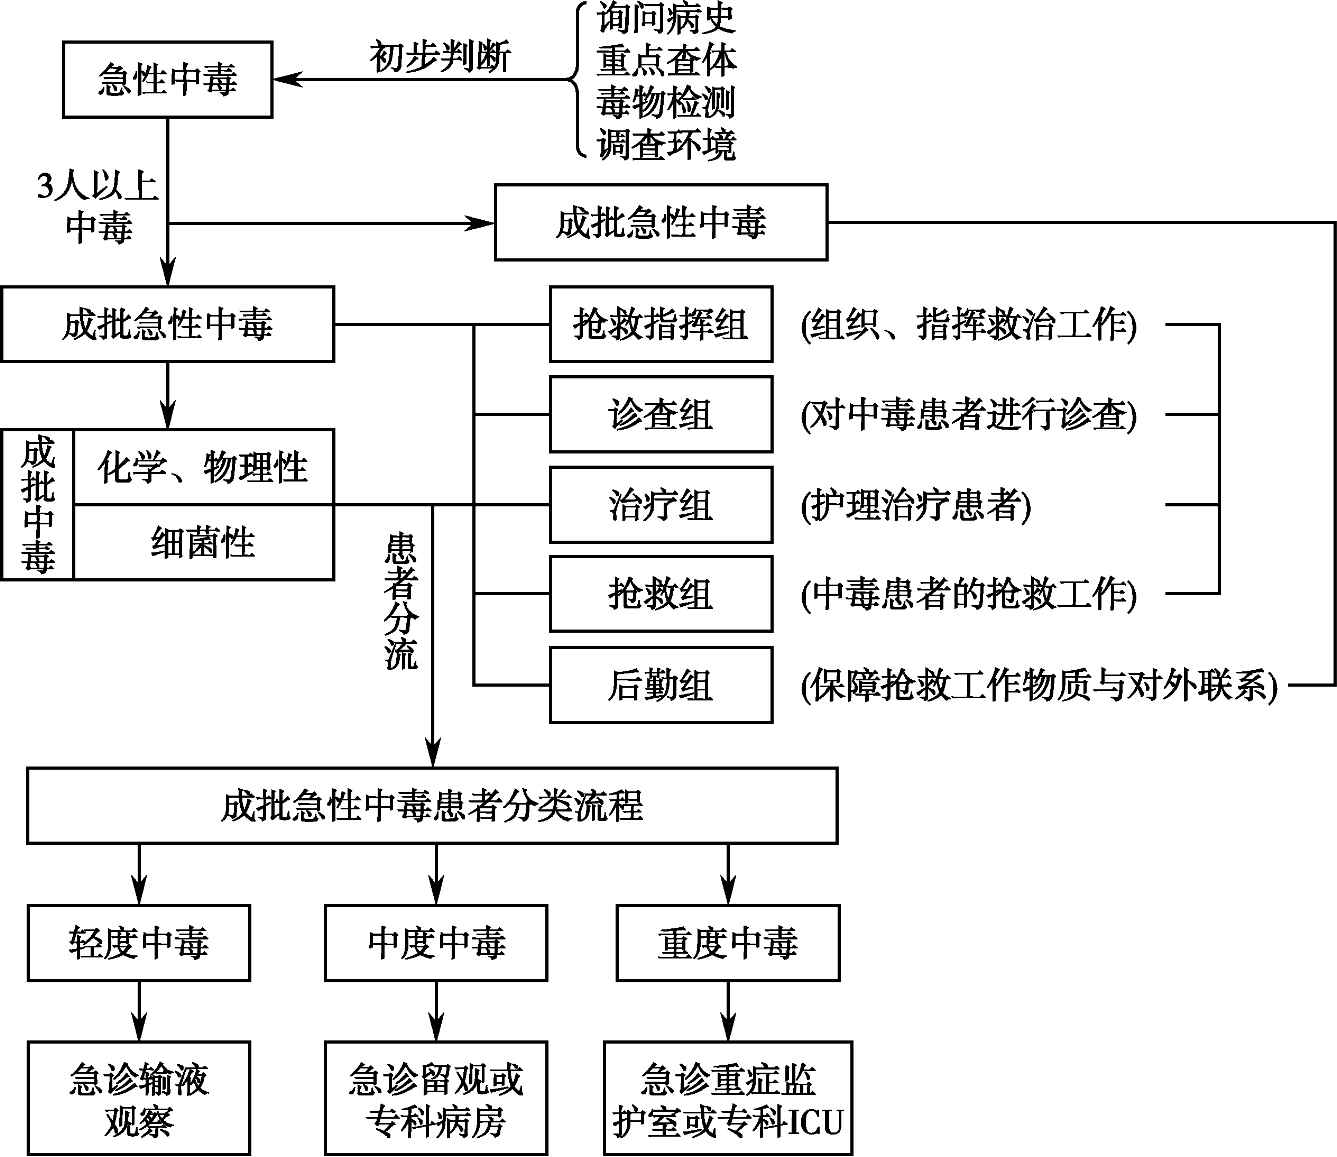
\includegraphics[width=4.20833in,height=3.64583in]{./images/Image00181.jpg}
 \captionsetup{justification=centering}
 \caption{急性中毒事件救治的组织指挥程序图}
 \label{fig53-1}
  \end{figure} 

3.用好现场救治急性中毒的主要措施
①有效地清除未吸收的毒物,尽快排除已吸收的毒物,如洗胃、利尿、导泻、血液灌流等。②及时足量使用特效解毒剂,做到早期、足量、联合使用,防止副作用。③严密观察病情变化,及时有效地进行对症处理。④早期脏器功能支持,防止发生MODS,主要做好呼吸功能、心功能、肾功能、脑功能的维持,管好内环境,防止感染和消化道出血。

4.急性中毒事件救治的组织指挥程序见图\ref{fig53-1}。

\protect\hypertarget{text00131.html}{}{}

\chapter{急性药物中毒}

\section{急性毒品中毒}

毒品(narcotics)是指国家规定管制的能使人成瘾的麻醉(镇痛)药(narcotic
analgesics)和精神药(psychotropic
drugs),该类物质具有成瘾(或依赖)性、危害性和非法性。1997年修订的我国《刑法》第357条规定:“毒品是指鸦片、海洛因、甲基苯丙胺(冰毒)、吗啡、大麻、可卡因以及国家规定的其他能够使人形成瘾癖的麻醉品和精神药品”。短时间内滥用、误用或故意使用大量毒品超过个体耐受量产生相应临床表现时称为急性毒品中毒(acute
narcotics
intoxication)。急性毒品中毒常死于呼吸或循环衰竭,有时发生意外死亡。

通常将毒品分为麻醉(镇痛)药品和精神药品两大类。传统毒品主要是麻醉(镇痛)药品,包括阿片类、可卡因类(包括可卡因、古柯叶和古柯膏等)、大麻类(包括大麻叶、大麻树脂和大麻油等);而新型毒品主要是兴奋剂、致幻剂等精神药品。兴奋剂是加速和增强中枢神经系统活动,使人处于强烈兴奋状态,具有成瘾性的精神药品,其种类繁多,大多通过人工合成,常见的有苯丙胺(amphetamine,AA)及其苯丙胺类衍生物如甲基苯丙胺(metha
mphetamine,MA,俗称冰毒)、3,4-亚甲二氧基苯丙胺(3,4-methylene
dioxyamphetamine,MDA)、3,4-亚甲二氧基甲基苯丙胺(MDMA,俗称摇头丸)等;致幻剂包括麦角二乙胺(lysergide)、苯环已哌啶(phencyclidine)、西洛西宾和麦司卡林等。K粉(氯胺酮,ketamine)是苯环己哌啶衍生物,属于一类精神药品。绝大多数毒品中毒为过量滥用引起,滥用方式包括口服、吸入(如鼻吸、烟吸或烫吸)、注射(如皮下、肌内、静脉或动脉)或黏膜摩擦(如口腔、鼻腔或直肠)。有时误食、误用或故意大量使用也可中毒。毒品中毒也包括治疗用药过量或频繁用药超过人体耐受所致。

\subsubsection{阿片类药物中毒}

阿片类药物为麻醉性镇痛药,常见有吗啡(morphine)、哌替啶(pethidine,度冷丁)、可待因、二醋吗啡(heroin,海洛因)、美沙酮(methadone)、芬太尼(fentanyl)、舒芬太尼(sufentanil)及二氢埃托啡(dihydroetorphine,DHE)等,以及其粗制剂阿片、复方樟脑酊等。阿片类药物的主要作用是抑制中枢神经系统和兴奋胃肠道等平滑肌器官,在镇痛的同时,还可引起欣快感,患者感到精神愉快、舒适,一切不适的感觉、痛苦、烦恼等都被暂时消除,诱使患者重复用药,导致成瘾。一次误服大量或频繁应用可致中毒。吗啡中毒量成人为0.06g,致死量为0.25g;干阿片(含10\%的吗啡)的致死量为吗啡的10倍,其口服致死量2~5g;海洛因中毒剂量0.05~0.10g,致死量0.75~1.2g。可待因毒性为吗啡的1/4,其中毒剂量为0.2g,致死量0.8g。哌替啶致死量1.0g。

\hypertarget{text00131.htmlux5cux23CHP5-2-1-1-1}{}
(一) 病因与中毒机制

天然的阿片生物碱
,如吗啡等口服后吸收良好,皮下注射或肌注后吸收较快;给药后30分钟左右即可吸收60\%;药物主要在肝脏代谢,其代谢产物的90\%于24小时内由肾脏排出,48小时尿中仅有微量;少量经由乳汁、胆汁等途径排出,尚可通过胎盘屏障进入胎儿体内。阿片类药物对呼吸均有抑制作用,其抑制程度与剂量正相关。对神经系统的作用各有侧重,如阿片、吗啡等对中枢神经系统先有兴奋,以后抑制,但以抑制为主。中毒患者先呈兴奋状态,继则抑制大脑皮质的高级中枢,以后涉及延髓,抑制呼吸中枢和兴奋催吐化学感受区,最后使脊髓的兴奋增强。大剂量吗啡尚可抑制延髓血管运动中枢和释放组胺,使周围血管扩张而导致低血压和心动过缓。而可待因、哌替啶等则对大脑皮质中枢和延髓的抑制较弱,兴奋脊髓的作用较强。本类药物对支气管、胆管、输尿管都有兴奋作用,并能提高胃肠道平滑肌及其括约肌张力,减低胃肠蠕动。原有慢性病如肝病、肺气肿、支气管哮喘、贫血、甲状腺或肾上腺皮质功能减退症等患者均更易发生中毒。与酒精饮料同服,即使治疗剂量吗啡,也有发生中毒可能。巴比妥类及其他催眠药物与本类药物均有协同作用,合用时要谨慎为之。

\hypertarget{text00131.htmlux5cux23CHP5-2-1-1-2}{}
(二) 诊断

\paragraph{病史}

有本类药物应用或吸食史。非法滥用中毒者往往不易询问出病史,但查体可发现用毒品的痕迹,如经口鼻烫吸者,常见鼻黏膜充血、鼻中隔溃疡或穿孔;经皮肤或静脉吸食者可见注射部位皮肤有多处注射痕迹。

\paragraph{临床表现特点}

此类药物重度中毒时常发生昏迷、呼吸抑制和瞳孔缩小等改变。吗啡中毒典型表现为昏迷、瞳孔缩小或针尖样瞳孔和呼吸抑制(每分钟仅有2~4次呼吸,潮气量无明显变化)“三联征”,并伴有发绀和血压下降;海洛因中毒时除具有吗啡中毒“三联征”外,并伴有严重心律失常、呼吸浅快和非心源性肺水肿;哌替定中毒时除血压降低、昏迷和呼吸抑制外,与吗啡中毒不同的是心动过速、瞳孔散大、抽搐、惊厥和谵妄等;芬太尼等常引起胸壁肌强直;美沙酮尚可出现失明、下肢瘫痪等。重度急性中毒12小时内多死于呼吸衰竭,超过48小时存活者,预后良好。轻度急性中毒患者有头痛、头晕、恶心、呕吐、兴奋或抑郁。患者有幻想,失去时间和空间感觉,并可有便秘、尿潴留及血糖增高等。慢性中毒(阿片或吗啡瘾)表现为食欲不振、便秘、消瘦、衰老及性功能减退。戒绝药物时有精神萎靡、呵欠、流泪、冷汗、失眠,以致虚脱等表现。

\paragraph{辅助检查}

①毒物检测:尿或胃内容物、血液检测到毒物,有助于确立诊断。②动脉血气分析:严重麻醉性镇痛药中毒者表现为低氧血症和呼吸性酸中毒。③血液生化检查:血糖、电解质和肝肾功能检查。

\paragraph{鉴别诊断}

阿片类中毒出现谵妄时,可能为同时使用其他精神药物或合并脑部疾病所致。瞳孔缩小者还应与镇静催眠药、吩噻嗪类、有机磷农药、可乐定中毒或脑桥出血鉴别。海洛因常掺杂其他药如奎宁、咖啡因、地西泮等,以致中毒表现不典型,此时应想到掺杂物的影响。还须鉴别的是重症海洛因戒断综合征:有明确的吸毒史,如患者被发现时已陷入昏迷,而昏迷前是否应用毒品难以明确的情况下,鉴别有一定困难。重度海洛因戒断者一般无瞳孔缩小,以呼吸浅速为主要特征,每分钟可达60次以上,与海洛因中毒成鲜明对比,据此可以鉴别。本综合征用纳洛酮无效,反可使病情加重,使昏迷程度加深;应用吗啡后(一般10~20mg),呼吸可迅速改善,由50~60次/分钟降至20~30次/分钟,各种反射改善并很快清醒。

\hypertarget{text00131.htmlux5cux23CHP5-2-1-1-3}{}
(三) 治疗

\paragraph{清除毒物}

发现中毒患者后,首先确定中毒途径,以便尽速排除毒物。口服中毒患者以0.02\%~0.05\%高锰酸钾溶液反复洗胃,洗胃后由胃管灌入50~100g活性炭悬浮液,并灌服50\%硫酸钠50ml导泻。

\paragraph{吗啡拮抗剂}

①纳洛酮:可静脉、肌内、皮下或气管内给药。阿片类中毒伴呼吸衰竭者立即静注2.0mg;阿片成瘾中毒者3~10分钟重复,非成瘾中毒者2~3分钟重复应用。若纳洛酮总量已达20mg仍无效时应注意合并非阿片类毒品(如巴比妥类等)中毒、头部外伤、其他中枢神经系统疾病和严重缺氧性脑损害。长半衰期阿片类(如美沙酮)或强效阿片类(如芬太尼)中毒时需静脉输注纳洛酮(2.0~4.0mg加入250ml液体中静滴)。纳洛酮对吗啡的拮抗作用是烯丙吗啡的30倍,较左洛啡烷强6倍。1mg纳洛酮能对抗静脉注射25mg海洛因作用。纳洛酮对芬太尼中毒所致的肌肉强直有效,但不能拮抗哌替啶中毒引起的癫痫发作和惊厥,对海洛因、美沙酮中毒引起的非心源性肺水肿无效。②烯丙吗啡(纳洛芬):5~10mg/次,静注或肌注,必要时10~15分钟后可重复给予,总量不超过40mg。③左洛啡烷:首次1~2mg静脉注射,继而5~15分钟注射0.5mg,连用1~2次。

\paragraph{对症支持疗法}

保持呼吸道通畅,吸氧,适当应用呼吸兴奋剂,如安钠咖(苯甲酸钠咖啡因)0.5g肌注,每2~4小时1次;尼可刹米(可拉明)0.375~0.75g或洛贝林3~
15mg肌注或静注。必要时气管插管人工呼吸,釆用PEEP可有效纠正海洛因和美沙酮中毒引起的非心源性肺水肿,同时用血管扩张药和呋塞米,禁用氨茶碱。输液,纠正休克,抗生素应用等。重度中毒患者可同时予以血液净化治疗,但效果不确切。

\subsubsection{苯丙胺类兴奋剂中毒}

苯丙胺类中枢兴奋剂(ATS)包括苯丙胺、甲基苯丙胺(俗称冰毒)、3,4-亚甲二氧基苯丙胺(MDA)、3,4-亚甲二氧基甲基苯丙胺(俗称摇头丸)等。当前滥用的“摇头丸”其主要成分含甲基苯丙胺、3,4-亚甲二氧基甲基苯丙胺、麻黄碱和氯胺酮等,实质是甲基苯丙胺类的混合物。其药丸颜色有粉红、黄色、橘红色、黑色等,别名有“舞会药,拥抱药、亚当、蓝精灵、雅皮士”等。ATS是一种非儿茶酚胺的拟交感神经胺低分子量化合物,吸收后易通过血脑屏障,主要作用机制是促进脑内儿茶酚胺递质(多巴胺和去甲肾上腺素)释放,减少抑制性神经递质5-羟色胺的含量,产生神经兴奋和欣快感。可以吸入、口服、注射等方法进入体内。此类药物急性中毒量个体差异很大,一般静注甲基苯丙胺10mg数分钟可出现急性中毒症状,吸毒者静注30~50mg及耐药者静注1000mg以上才能发生中毒,成人苯丙胺口服致死量为20~25mg/kg。

\hypertarget{text00131.htmlux5cux23CHP5-2-1-2-1}{}
(一) 诊断

\paragraph{病史}

有明确的吸食此类毒品的病史。精神药品滥用常见于经常出入特殊社交和娱乐场所的青年人。

\paragraph{临床表现特点}

①急性中毒:常为吸食过量或企图自杀所致。临床表现为中枢神经和交感神经过度兴奋的症状。轻度中毒表现为兴奋、躁动、血压升高、脉搏加快、出汗、口渴、呼吸困难、震颤、反射亢进、头痛等症状;中度中毒出现错乱、谵妄、幻听、幻视、被害妄想等精神症状。重度中毒时,可出现胸痛、心律失常、循环衰竭、代谢性酸中毒、DIC、高热、昏迷甚至死亡。另外,ATS可引起肺动脉高压、心肌梗死、心肌病、高血压、心律失常、颅内出血、猝死等。②慢性中毒:慢性中毒比急性中毒更为常见。通常以重度的神经异常症状为特征,而且还可出现明显的暴力、伤人和杀人等犯罪倾向,为重大的社会问题。冰毒引起的精神异常可分为四类:分裂样精神病、躁狂-抑郁状态、分裂-躁狂抑郁混合、病态人格样状态。除上述精神异常外,冰毒还引起性格改变:表现为无为、漫不经心、轻浮、粗暴、威胁言行或孩童样性格等。

根据吸食史及临床表现,一般不难作出ATS中毒的临床诊断,必要时可测定血、尿中ATS及其代谢产物加以确诊。

\hypertarget{text00131.htmlux5cux23CHP5-2-1-2-2}{}
(二) 治疗

1.终止毒物吸收,加速毒物排泄
如系口服所致,可行催吐、洗胃、灌服活性炭及导泻等措施,必要时可行血液灌流,以清除血中毒物。

2.对症治疗
无特效解毒剂,主要为对症治疗,防治并发症。包括以下措施:①保持呼吸道通畅:应及时清除口、鼻腔的内分泌物及呕吐物,对频发抽搐、呼吸困难者,应及时行气管插管以防窒息;必要时行机械通气。②对昏迷者,可用纳洛酮。③急性中毒患者常出现高热、代谢性酸中毒和肌痉挛症状,应足量补液,维持水、电解质平衡,碱化尿液,利尿,以促进毒物排泄。④恶性高热者除物理降温(冰敷、醇浴)外,应用肌肉松弛剂是控制高体温的有效方法,可静脉缓慢注射硫喷妥钠0.1~0.2g或琥珀酰胆碱,必要时可重复,注意呼吸和肌肉松弛情况。⑤对极度兴奋或烦躁的患者,可用氟哌啶醇2~5mg每4~6小时肌注一次或以50\%葡萄糖液稀释后在1~2分钟内缓慢静注,必要时加量应用,待好转后改口服,每次1~2mg,每日3次。高血压和中枢神经兴奋症状可用氯丙嗪1mg/kg肌注,4~6小时一次。显著高血压可采用酚妥拉明或硝普钠。出现快速心律失常可用普萘洛尔。

\subsubsection{氯胺酮(K粉)中毒}

氯胺酮(ketamine,俗称K粉)是新的非巴比妥类静脉麻醉药。为中枢兴奋性氨基酸递质N-甲基-D-天门冬氨酸(NMDA)受体特异性拮抗药,选择性阻断痛觉冲动向丘脑-新皮质传导,具有镇痛作用;对脑干和边缘系统有兴奋作用,能使意识与感觉分离;对交感神经有兴奋作用,快速大剂量给予时抑制呼吸;尚有拮抗µ受体和激动κ受体作用。吸食者在K粉作用下会疯狂摇头,造成心力衰竭、呼吸衰竭,若过量或长期吸食,对心、肺、神经系统均可造成致命损伤。氯胺酮起效迅速,吸入少量30秒后可致人昏迷,清醒后也不记起所发生的事,因而有人把氯胺酮又叫做“迷奸药”。

\hypertarget{text00131.htmlux5cux23CHP5-2-1-3-1}{}
(一) 诊断

\paragraph{病史}

有此类毒品明确的吸食史。

\paragraph{临床表现特点}

①精神、神经系统:表现为鲜明的梦幻觉、错觉、分离状态或分裂症状,尖叫、兴奋、烦躁不安、定向障碍、认知障碍、易激惹行为、呕吐、流涎、谵妄、肌张力增加和颤抖等。部分人可出现复视、暂时失明持续可达15~30分钟。②心血管系统:氯胺酮可增加主动脉压、提升心率和心脏指数,还可增加脑血流和颅内压以及眼压。因此,心功能不全、有心血管疾病、严重高血压或伴脑出血、青光眼患者服用氯胺酮非常危险。③消化系统:恶心呕吐、腹胀、胃出血、急性胃扩张等。④呼吸系统:主要表现为呼吸抑制、呼吸暂停、喉痉挛、支气管痉挛、哮喘等。⑤变态反应:主要表现为急性荨麻疹、眼结膜水肿、喉头水肿、休克等,故有药物过敏史者易发生过敏性休克。

\hypertarget{text00131.htmlux5cux23CHP5-2-1-3-2}{}
(二) 治疗

与苯丙胺类兴奋剂中毒的治疗基本相同。

\subsubsection{可卡因中毒}

可卡因为古柯叶中提取的古柯碱,是一种脂溶性物质,为很强的中枢兴奋剂和古老的局麻药。有中枢兴奋和拟交感神经作用,通过使脑内5-羟色胺和多巴胺转运体失去活性产生作用。中毒剂量为20mg,致死量为1200mg,有时纯可卡因70mg能使70kg的成年人即刻死亡。静脉注射中毒可使心脏停搏。急性重症中毒时,表现奇痒难忍、肢体震颤、肌肉抽搐、癫痫大发作、体温和血压升高、瞳孔扩大、心率增快、呼吸急促和反射亢进等。无特异性治疗,主要是对症支持治疗。

\subsubsection{大麻中毒}

滥用最多的是印度大麻,含有主要的精神活性物质是四氢大麻酚、大麻二酚、大麻酚及其相应的酸。作用机制不详,急性中毒时与酒精作用相似,产生精神、呼吸和循环系统损害。长期应用产生精神依赖性,而非生理依赖性。一次大量吸食会引起急性中毒,表现精神和行为异常,如高热性谵妄、惊恐、躁动不安、意识障碍或昏迷。有的出现短暂抑郁状态,悲观绝望,有自杀念头。检查可见球结膜充血、心率增快和血压升高等。主要是对症支持治疗。

\protect\hypertarget{text00132.html}{}{}

\section{镇静催眠药中毒}

镇静催眠药物是抑制中枢神经系统引起镇静和催眠的药物。一般镇静催眠药小剂量镇静,中剂量催眠,大剂量麻醉,有的还有抗惊厥、抗精神病作用。一次服用大剂量可引起急性镇静催眠药中毒(acute
sedative-hypnotic
poisoning);长期滥用催眠药可引起耐药性和依赖性而导致慢性中毒;突然停药或减量可引起戒断综合征(withdrawal
syndrome)。镇静催眠药是临床上最常用的一类药物,由于其使用或管理不当所致的药物中毒也位居第一位。按照化学结构,本类药物可分为5类:①苯二氮{}
类;②巴比妥类;③醛类,如水合氯醛;④环吡咯酮类药物,如佐匹克隆(zopiclone,忆梦返)、唑吡坦(zolpidem,思诺思)等被认为是新一代的催眠药;⑤其他:包括氨基甲酸类:甲丙氨酯;溴化物:溴化钠、溴化钾。临床常用的镇静催眠药物有巴比妥类和苯二氮{}
类,不常用的有甲丙氨酯、格鲁米特、水合氯醛、甲喹酮等。

\subsubsection{苯二氮{} 类药物中毒}

苯二氮{} 类(benzodiaze
pines,BZD)药物是近年来迅速发展的一类镇静催眠药。与巴比妥类或其他类镇静催眠药比较,具有选择性高,安全范围大,对呼吸抑制小,不影响肝药酶活性,长期应用虽可产生耐受性与依赖性,但相对发生率低等优点,几乎取代了所有老药,成为应用最广泛的镇静催眠药,还常被用于抗癫痫、抗惊厥和全身麻醉等,因而本类药引起的急性过量中毒也最为常见,也是城市人群急性中毒最常见的原因。

\subsection{病因与中毒机制}

本类药物也称弱安定药,包括超短作用时(<
6小时)的三唑仑(triazolam,海乐神);短作用时(6~20小时)的阿普唑仑(alprazolam,佳静安定)、劳拉西泮(diazepam,氯羟安定,罗拉)、替马西泮(temazepam);中作用时(≥20小时)的地西泮(diazepam,安定)、氯氮{}
(chlordiazepoxide,利眠宁);长作用时(≥40小时)的氟西泮(flurazepam,氟安定)、普拉西泮(prazepam)等。本类药物是特异性BZD受体激动剂,该受体广泛分布于中枢神经细胞的突触部位(尤其是大脑边缘系统如杏仁核,与人的情绪、记忆密切相关),与γ-氨基丁酸(GABA)受体、氯离子通道形成复合物;激动BZD受体能增强GABA对氯离子通道的门控作用,使突触膜过度极化,最终增强GABA介导的中枢神经系统抑制作用。大剂量时除可抑制中枢神经系统外,还可抑制心血管系统。一次误服大量或长期内服较大剂量,可引起毒性反应;同时摄入乙醇、中枢抑制剂及环类抑制剂等可使其毒性增强。老年人对本类药物敏感性增高。因本类药物的中毒剂量与治疗剂量比值非常高,由本类药物中毒直接致死罕见,以利眠宁为例,成人的治疗口服量5~50mg,最小致死量约2g。

\subsection{诊断}

\paragraph{病史}

有误用或自服大剂量本类药物史。

\paragraph{临床表现特点}

服用本类药物过量者,有嗜睡、眩晕、乏力、运动失调,偶有中枢兴奋、锥体外系障碍及一时性精神错乱。老年体弱者易有晕厥。口服中毒剂量后,除上述症状外尚有昏迷、血压下降及呼吸抑制。同服其他中枢抑制剂或乙醇者,存在基础心肺疾患者或老年人可发生长时间深昏迷、致死性呼吸抑制或循环衰竭。静注速度过快、剂量过大,也可引起呼吸抑制。

\paragraph{实验室检查}

①毒物检测:对可疑中毒者,有条件时行血、尿定性试验;血药浓度测定对诊断有意义,但与临床毒性表现相关性差;②其他检查:对重症患者尚应进行肝肾功能、血清电解质、动脉血气及心电图检查。

\paragraph{鉴别诊断}

应与其他原因的昏迷如肝性脑病、糖尿病、急性脑卒中等相鉴别。若怀疑本类药物急性中毒,可用氟马西尼作诊断性试验(见下述治疗部分)。

\subsection{治疗}

\paragraph{洗胃}

口服中毒者,立即用微温清水或1∶5000高锰酸钾溶液洗胃,然后用硫酸钠导泻。

\paragraph{对症支持治疗}

①重症患者应监测生命体征,保持呼吸道通畅,高流量吸氧;②维持循环稳定:低血压者经静脉输液多可恢复,少数血压仍低者,可加用血管活性药物如多巴胺或间羟胺静滴;③昏迷患者应注意保暖,维持水、电解质平衡,防治肺部及泌尿系感染。

\paragraph{特异性解毒剂}

氟马西尼(flumazenil,安易醒)是BZD受体特异性拮抗剂,能与BZD类药物竞争受体结合部位,从而逆转或减轻其中枢抑制作用。昏迷患者可于静注后l分钟清醒,因而本品适用于可疑BZD类药物中毒的诊断和重症BZD类中毒者的急救。对乙醇和阿片类药物中毒无效。用药方法:先用0.2~0.3mg静注,继之以0.2mg/min静注直至有反应或达2mg。因本品半衰期短(0.7~1.3小时),故对有效者每小时应重复给药0.1~0.4mg,以防症状复发。曾经长期使用BZD类药物的患者,如快速注射本品,会出现戒断症状,如焦虑、心悸、恐惧等,故应缓慢注射;戒断症状较重者,可缓慢注射地西泮5mg。

\paragraph{纳洛酮治疗}

纳洛酮是阿片受体特异拮抗剂,能阻断和逆转内阿片肽的毒性作用,可使患者清醒时间明显缩短,心率加快,血压升高,可作为抢救镇静催眠药急性中毒的首选药物之一。用药方法为依病情0.4~1.2mg用静注,必要时30分钟重复1次,或用2~4mg加入5\%~10\%葡萄糖液100~250ml中静滴。

\paragraph{中药醒脑静注射液}

中药醒脑静注射液是由麝香、冰片、郁金、栀子等提取精制而成的中药针剂。具有醒神止痉、清热凉血、行气活血等功效。可显著缩短镇静催眠药中毒的意识障碍时间,具有极好的促醒功效。应用安全,治疗前后血压、心率等血流动力学指标无显著变化。常用5~20ml加入5\%~10\%葡萄糖液250~500ml中静滴。

\paragraph{胞磷胆碱}

胞磷胆碱是脑代谢活化剂,通过促进卵磷脂的合成而促进脑组织代谢,并降低脑血管阻力,增加脑血流,改善大脑物质代谢,从而改善大脑功能。同时,可增强脑干网状结构上行激活系统功能,促进苏醒。用法:0.25~0.5g/d加入5\%~10\%葡萄糖液250~500ml中静滴。

\paragraph{血液净化疗法}

对重症患者上述治疗措施无效时,可考虑血液灌流治疗,部分病例可取得较好效果。

既往身体健康的轻度中毒患者经急诊处理后神志清楚、生命体征稳定,可回家休息。中度~重度中毒的患者应留院观察治疗;对合并其他药物中毒和(或)伴有脏器功能障碍的重度中毒患者应入ICU监护治疗。

\subsubsection{巴比妥类药物中毒}

\subsection{病因与中毒机制}

巴比妥类(barbiturates)药物曾经是常用的镇静和催眠剂,是巴比妥酸的衍生物。由于苯二氮{}
类已成为临床最常用的镇静催眠药物,故巴比妥类药物中毒已逐渐少见。人工合成的巴比妥类药物有2500余种,其中临床应用的有10种左右。临床常用的巴比妥类药物,根据其起效时间和作用持续时间可分为四类:①长效类:包括巴比妥(barbitone)和苯巴比妥(鲁米那,phenobarbital,luminal),开始作用时间30~60分钟,作用持续时间6~8小时;其催眠剂量分别为0.3~0.6g/次和0.03~0.1g/次。②中效类:包括异戊巴比妥(阿米妥,amobarbital,amytal)和戊巴比妥(pentobarbital),开始作用时间15~30分钟,作用持续时间4~6小时,其催眠剂量为0.2~0.4g/次。③短效类:包括司可巴比妥(速可眠,secobarbital,seconal),开始作用时间15~20分钟,作用持续时间2~3小时,其催眠剂量为0.1~0.2g/次。④超短效类:主要为硫喷妥钠(sodium
thiopental),开始作用时间30秒内,作用持续时间30~45分钟,其催眠剂量0.5~1.0g/次。一般由于误服过量或因其他原因应用过多而引起中毒,临床上以中枢神经系统的抑制为主要表现。半衰期短、脂溶性大的巴比妥类比半衰期长、脂溶性低的巴比妥类毒性大,如苯巴比妥的口服致死量为6~10g,而司可巴比妥、异戊巴比妥约为3g。发生毒作用时的血内药物浓度:中、短效为30mg/L,长效为80~100mg/L。

口服巴比妥类,自肠道吸收较快,其钠盐的水溶液易自肌肉吸收,在体内可分布于一切组织和体液中,也易透过胎盘而分布到胎儿组织。组织中的浓度几乎与血浆中的浓度相同,故血中浓度能够代表组织中的含量。进入脑组织的速度取决于脂溶性的高低,脂溶性高者(如司可巴比妥)容易进入脑组织,因此作用快;脂溶性低者(如苯巴比妥)则作用慢。巴比妥类在体内主要经两种方式消除,一种是经肝脏氧化,另一种是以原型由肾脏排出。中及短效类药物主要经肝脏代谢,因此维持时间短;苯巴比妥主要经肾脏排出,因肾小管的再吸收,排泄较慢,故作用较持久。如巴比妥钠75\%以原型由尿中排出,在第8~12天仍可由尿中检出痕迹量。硫喷妥钠在肝脏内几乎全部被氧化破坏,仅0.3\%以原型从尿中排出。苯巴比妥有48\%左右在肝脏氧化,15\%~20\%以原型由尿排出,其排泄速率取决于尿的pH,当尿呈酸性时,苯巴比妥有一部分不解离而被肾小管重吸收,当尿呈碱性时则被解离而随尿排出。当服用大量巴比妥或苯巴比妥后,血中浓度下降速率为24小时降低10\%~15\%,戊巴比妥与司可巴比妥24小时降低50\%~70\%。乙醇在增加巴比妥类吸收速率的同时又可阻碍其在肝的代谢而延长巴比妥类的作用,加重其毒性作用。

本类药物能抑制丙酮酸氧化酶系统,从而抑制中枢神经系统,特别是对大脑皮质、下丘脑和脑干网状结构上行激活系统有抑制作用。随着剂量由小到大,抑制程度由浅到深,反射功能逐渐消失,表现为镇静→催眠→止惊→麻醉作用。大剂量巴比妥类可直接抑制延髓呼吸中枢,导致呼吸衰竭,是致死的主要原因;抑制血管运动中枢,使周围血管扩张,发生休克。某些短效巴比妥类药物中毒早期,即可引起肺水肿;应用长效巴比妥类药物,在中毒后期,可发生坠积性肺炎。对中枢神经系统的抑制程度取决于其类型(长效或速效)、剂量、用法(口服或注射)和机体的耐受性。其作用速度、持续时间与其脂溶性大小有关,而其脂溶性与第5位碳原子取代基团侧链的结构有关,取代基团侧链加长或有分支、不饱和链,或第2位碳上的氧原子被硫取代,则脂溶性增高,其作用快,强度大,持续时间短(如司可巴比妥、硫喷妥钠);如侧链为短链或为苯环,则脂溶性降低,作用慢,强度低,持续时间长(如巴比妥)。精神抑郁,肝、肾功能不全和饮酒后,易致中毒或使病情更加严重。

\subsection{诊断}

\paragraph{毒物接触史}

有误服或应用大量巴比妥类药物史,或现场查出有残留的巴比妥类药物。

\paragraph{临床表现特点}

中毒症状的轻重,取决于进入人体内药物的种类、途径、剂量、作用长短,以及抢救时间的早晚和患者肝、肾功能及全身状态等。依病情轻重分为:

\hypertarget{text00132.htmlux5cux23CHP5-2-2-2-2-2-1}{}
(1) 轻度中毒:

发生于2~5倍催眠剂量。患者入睡,推动可以叫醒,反应迟钝,言语不清,有判断及定向力障碍。

\hypertarget{text00132.htmlux5cux23CHP5-2-2-2-2-2-2}{}
(2) 中度中毒:

发生于5~10倍催眠剂量。患者沉睡或进入昏迷状态,强刺激虽能唤醒,但并非全醒,不能言语,旋即又沉睡。呼吸略慢,眼球有震颤。

\hypertarget{text00132.htmlux5cux23CHP5-2-2-2-2-2-3}{}
(3) 重度中毒:

发生于误服10~20倍催眠剂量。患者深度昏迷,呼吸浅而慢,有时呈陈-施呼吸。短效类药物中毒偶有肺水肿。吸入性肺炎很常见。脉搏细速,血压下降,严重者发生休克。由于药物对下丘脑垂体系统作用的结果,ADH分泌增加,患者有少尿。昏迷早期有四肢强直,腱反射亢进,锥体束征阳性;后期全身弛缓,各种反射消失,瞳孔缩小,对光无反应。常伴有肝、肾功能损害的表现。

对本类药物有超敏反应者,可出现各种形态的皮疹,如猩红热样疹、麻疹样疹、荨麻疹、疱疹等,偶有剥脱性皮炎。

\paragraph{辅助检查}

血液、呕吐物及尿液巴比妥类药物测定,有助于确立诊断。对重度中毒患者应做血气分析及肝、肾功能检查。

\paragraph{鉴别诊断}

巴比妥类药物中毒是药物中毒致昏迷者中常见的原因之一,因此,必须与其他药物(如吗啡类、水合氯醛)中毒和其他原因的昏迷如肝性脑病、糖尿病、急性脑卒中等相鉴别。

\subsection{治疗}

治疗重点在于维持呼吸、循环和肾脏功能。

1.清除毒物
口服中毒者早期用1∶5000高锰酸钾溶液或大量清水洗胃,服药量大者即使超过4~6小时仍需洗胃,以清除残留毒物。洗胃后由胃管灌入硫酸钠30g导泻及活性炭混悬液于胃内,以吸附未被吸收的药物。注意忌用硫酸镁导泻,因镁离子可能被部分吸收而加重中枢神经系统的抑制。

2.促进巴比妥类药物的排泄
有下列药物:①静脉滴注5\%~10\%葡萄糖液及生理盐水,每日3000~4000ml;②利尿剂:巴比妥类由肾小球滤过之后,部分由肾小管重吸收,但肾脏对巴比妥类的廓清是随尿量的增多而增加的,尤其对长效类更如此。利尿可使血浆中巴比妥类的浓度下降加快,缩短患者的昏迷时间。可快速滴注渗透性利尿剂甘露醇(0.5g/kg),每日1~2次;亦可用呋塞米(速尿)40~80mg静注,要求每小时尿量达250ml以上。③碱性尿液:有利于巴比妥类由周围组织释出并经肾脏排泄。对长效药物作用较大,对短效者作用较差。实验研究发现通过碱化尿液(pH
7.8~8.0)可使苯巴比妥的排出增加10倍。静脉滴注4\%~5\%碳酸氢钠液100~200ml,若同时加用乙酰唑胺(0.25g,每6小时一次),可能会使尿液最大限度地碱化(pH
8.0)。须注意发生代谢性碱中毒和肺水肿的危险。

3.维持呼吸与循环功能
保证气道通畅和充分的换气,持续给氧;必要时气管插管或气管切开,人工呼吸机呼吸。尽速纠正低氧血症和酸中毒,有利于心血管功能的恢复。如有休克应及时抗休克治疗,巴比妥类药物中毒引起的休克为中枢抑制所致,缩血管药物如去甲肾上腺素、间羟胺等常有较好抗休克效果。

4.血液净化疗法
对严重中效药物中毒或肾功能不全者,可考虑(血液或腹膜)透析疗法,以排除体内过多毒物,纠正高钾血症和酸中毒,降低氮质血症。对短效类药物中毒,利尿和透析的效果不理想,因该类药物与血浆蛋白结合较多,并且主要在肝脏代谢。病情危重或有肝功能不全时可试用活性炭树脂血液灌流。当患者服用苯巴比妥量>
5g或血苯巴比妥浓度> 80mg/L时,应尽早予以血液净化治疗,首选血液灌流。

5.纳洛酮治疗
纳洛酮是阿片受体特异拮抗剂,能阻断和逆转内阿片肽的毒性作用,可使患者清醒时间明显缩短,心率加快,血压升高,可作为抢救镇静催眠药急性中毒的首选药物之一。用药方法:轻度0.4~0.8mg,中度0.8~1.2mg,重度中毒1.2~2mg静注。必要时30分钟重复1次,或用2~4mg加入5\%~10\%葡萄糖液100~250ml中静滴。

6.中药醒脑静注射液也有一定的催醒作用。

7.中枢兴奋剂的应用
这类药物并非解毒剂,不参与巴比妥类药物的代谢或排泄,仅在深昏迷或有呼吸抑制现象时使用,其目的在于恢复和保持反射,使机体在消除过量的巴比妥类药物以后逐渐苏醒。不可企图用中枢兴奋剂使患者完全清醒,因该类药物易致惊厥,增加机体耗氧量,反而加重中枢抑制和衰竭。若中枢兴奋剂使用过量引起惊厥,可注射短效或超短效的巴比妥类,以解除其作用。当患者有:①深昏迷,处于完全无反射状态;②明显呼吸衰竭;③积极抢救48小时患者仍昏迷不醒等三项中一项时才可考虑酌情选用下列中枢兴奋剂中一种:①贝美格(美解眠):100~200mg加入葡萄糖液250~500ml中静滴,或用50mg静注,3~5分钟1次,直至血压、呼吸和反射恢复正常。②尼可刹米(可拉明):可用0.375g静注、肌注,或3~5支(0.375g/支)加入液体中静滴,直至患者稍清醒,反射恢复和出现肌肉震颤。③多沙普仑(doxapram):20mg
用5\%葡萄糖注射液稀释至1mg/ml后缓慢静注,或100mg加入5\%葡萄糖注射液100~250ml中静滴,每小时用量不超过300mg。

8.对症支持疗法 如抗感染、维持水电解质平衡、防治心力衰竭、脑水肿等。

本类药物中毒的患者应留院观察治疗;重度中毒患者应入ICU监护治疗。

\subsubsection{其他镇静催眠药物中毒}

其他镇静催眠药物是指巴比妥类和苯二氮{}
类以外的镇静催眠药物。现临床少用的有甲丙氨酯(meprobamate,眠尔通,安宁,安乐神,氨甲丙二酯)、格鲁米特(glutethimide,导眠能、多利丹)、水合氯醛(chloral
hydrate)、甲喹酮(methaqualone,安眠酮,海米那,眠可欣)等。

\hypertarget{text00132.htmlux5cux23CHP5-2-2-3-1}{}
(一) 甲丙氨酯中毒

甲丙氨酯在小肠吸收完全
,治疗剂量口服后1小时能被完全吸收,在服用大量时吸收约持续1~13小时,平均为4小时;肌肉注射在10~15分钟内吸收。在体内约15\%与血浆蛋白结合,在肝脏迅速降解后从肾脏排出,一般24~36小时完全排出。服治疗剂量时的t\textsubscript{l/2}
约8小时,超量服用时t\textsubscript{1/2}
延长至12小时左右。甲丙氨酯中毒原因多为自杀吞服过量,成人口服中毒量约为8g,最小致死量约为12~40g。中毒血药浓度值为60~100μg/ml,致死血药浓度值>
200μg/ml。甲丙氨酯中毒表现与巴比妥类药物中毒相似,严重的患者表现为心动过速、低血压、心律不齐、休克.呼吸衰竭、肺水肿,甚至昏迷。中毒剂量在不同的患者差别较大。长期服用可出现慢性中毒,其中毒剂量要比急性中毒时大,多表现为眩晕、共济失调、言语不清等。急诊处理要点:①口服中毒者立即洗胃,并用硫酸钠导泻。用胃管洗胃时要注意甲丙氨酯在胃内形成胃石影响洗胃效果。②静脉输液以促进排泄。③出现抽搐者用地西泮或苯巴比妥治疗。④血液透析和血液净化用于危重患者的治疗。⑤对症与支持治疗。

\hypertarget{text00132.htmlux5cux23CHP5-2-2-3-2}{}
(二) 格鲁米特中毒

格鲁米特呈脂溶性
,消化道吸收极不规律。一般多在服药后30分钟起效,持续4~8小时。与血浆蛋白结合率为35\%~59\%,在肝脏代谢为水溶性高的物质后从肾脏排出,体内t\textsubscript{1/2}
为10~12小时,但在达稳态浓度后,t\textsubscript{1/2}
延长至22小时;中毒量时t\textsubscript{1/2}
进一步延长。格鲁米特成人中毒量> 3g,致死量>
5~10g,儿童中毒量为500mg。格鲁米特中毒临床表现特点:①意识障碍,意识障碍呈周期性波动,共济失调,严重者可有抽搐、昏迷。②循环系统抑制作用突出,多表现为肺水肿、低血压休克。③可出现视物模糊,眼球震颤、瞳孔扩大、对光反射迟钝、视乳头水肿、口干、便秘、尿潴留等。④成瘾性,突然停药可产生戒断综合征。急诊处理要点:①口服中毒者立即洗胃,并用硫酸钠导泻。格鲁米特中毒所引起的副交感神经作用及吸收的不规则性,使其在胃内停留时间较长,所以即使就诊较迟也要尽量洗胃。②静脉输液以促进排泄。③出现抽搐者给予地西泮或苯巴比妥治疗;应用呋塞米等利尿剂及糖皮质激素治疗脑水肿。④重症患者应尽早行血液净化治疗(血液透析或血液灌流)。⑤对症与支持治疗。

\hypertarget{text00132.htmlux5cux23CHP5-2-2-3-3}{}
(三) 水合氯醛中毒

水合氯醛在胃内吸收迅速
,血浆蛋白结合率约40\%,在肝脏经乙醇脱氢酶的作用降解为三氯乙醇(活性成分)、三氯乙酸及数种葡糖苷酸。三氯乙酸的t\textsubscript{1/2}
为34~35小时,三氯乙醇的t\textsubscript{1/2}
为10~13天。水合氯醛中毒常见原因为误服、自杀吞服过量和用药过量引起。水合氯醛成人中毒量为4~5g,儿童中毒量为1.5g,成人最小致死量为5~10g。中毒血药浓度值为100μg/ml,致死血药浓度值为250μg/ml。水合氯醛中毒临床表现特点:①治疗量下可出现消化道刺激症状,如恶心、呕吐、腹泻等;②过量服用后2~3小时出现明显的中毒症状,呼出气体有梨样气味,初期瞳孔缩小,后期可扩大;并出现低血压、心律异常,肺水肿、呼吸困难、组织缺氧、言语表达异常、抽搐、昏迷等表现。③肝肾功能损害表现。急诊处理要点:①口服中毒者立即洗胃,并用硫酸钠导泻。由直肠给药引起的中毒者应即时洗肠。水合氯醛中毒时洗胃要注意防止食管、胃穿孔。②静脉输液以促进排泄。③对出现室性心律不齐的患者可应用β受体阻滞剂,如普萘洛尔(心得安),也可用利多卡因。氟马西尼对改善呼吸衰竭和昏迷有一定疗效。④重症患者应尽早行血液净化治疗(血液透析或血液灌流)。⑤对症与支持治疗。

\hypertarget{text00132.htmlux5cux23CHP5-2-2-3-4}{}
(四) 甲喹酮中毒

甲喹酮脂溶性高
,口服后2小时内约全部被吸收,70\%~90\%与血浆蛋白结合,在肝脏羟化酶的作用下完全降解,降解产物主要通过肾脏排出。治疗剂量血中t\textsubscript{1/2}
为33~40小时,超量服用时t\textsubscript{1/2}
延长。甲喹酮中毒原因多为自杀吞服过量引起。甲喹酮(安眠酮)成人口服>
800mg可出现中毒,最小致死剂量为8g,儿童1片即可出现中毒,一般成人致死量为10~20g。甲喹酮中毒临床表现特点:①小量可出现欣快感,无力、恶心、呕吐、上腹部不适、流涎、共济失调、意识障碍等。②锥体束征,肌阵挛、肌张力增高,腱反射亢进,肌束震颤及全身肌肉抽动,甚至癫痫大发作。③可出现心动过速、低血压等改变。④有成瘾性,突然停药可出现戒断症状。⑤部分患者可出现非心源性肺水肿。急诊处理要点:①口服中毒者立即洗胃,并用硫酸钠导泻。②静脉输液以促进排泄。③对症与支持治疗。④血液透析和血液净化多用于危重患者的治疗。

\subsubsection{戒断综合征}

各种镇静催眠药均可产生耐受性与依赖性,因而均可引起戒断综合征。长期服用苯二氮{}
类使苯二氮{} 类受体减少,是发生耐受的原因之一。长期服用苯二氮{}
类突然停药时,发生苯二氮{}
类受体密度上调而出现戒断综合征。巴比妥类、非巴比妥类以及乙醇发生耐受性、依赖性和戒断综合征的情况更为严重。发生依赖性的证据是停药后发生戒断综合征。戒断综合征的特点是出现与药理作用相反的症状,如停用巴比妥类出现躁动和癫痫样发作;停用苯二氮{}
类出现焦虑和睡眠障碍。

临表现特点:长期大剂量服用镇静催眠药患者,突然停药或迅速减少药量时,可发生戒断综合征。主要表现为自主神经兴奋性增高和轻重度神经和精神异常:①轻症:最后一次服药后1天内或数天内出现焦虑、易激动、失眠、头痛、厌食、无力和震颤。2~3天后达到高峰。可有恶心、呕吐和肌肉痉挛。②重症:突然停药后1~2天,有的在7~8天后出现癫痫样发作,有时出现幻觉、妄想、定向力丧失、高热和谵妄,数天至3周内恢复,患者用药量多为治疗量5倍以上,时间超过1个月。滥用巴比妥类者停药后发病较多、较早,且症状较重,出现癫痫样发作及轻躁狂状态者较多。滥用苯二氮{}
类者停药后发病较晚,症状较轻,以焦虑和失眠为主。

戒断综合征应与以下疾病鉴别:原发性癫痫以往有癫痫发作史;精神分裂症、酒精中毒均可有震颤和谵妄,但前者有既往史,后者有酗酒史。

治疗原则是用足量镇静催眠药控制戒断症状,稳定后,逐渐减少药量以至停药。具体方法是将原用短效药换成长效药如地西泮或苯巴比妥。地西泮10~20mg或苯巴比妥1.7mg/kg肌注,每小时1次,直至戒断症状消失。然后以其总量为一天量,分为3~4次口服,待情况稳定2天后,逐渐减少剂量。在减量时,每次给药前观察患者病情,若不出现眼球震颤、共济失调、言语含糊不清,即可减少5\%~10\%。一般在10~15天减完,停药。

\protect\hypertarget{text00133.html}{}{}

\section{抗精神病药物中毒}

抗精神病药物(antipsychotics)是指能治疗各类精神病及各种精神症状的药物,又称强安定剂或精神阻断剂。本类药物发展较快,出现了许多新型品种,现临床常用的除吩噻嗪类、硫杂蒽类与丁酰苯类外,还有一些苯二氮{}
类抗精神病药及新型结构的抗精神病药。此外还合成了一些长效制剂,如吩噻嗪类、硫杂蒽与丁酰苯类的酯化物。

\paragraph{吩噻嗪类}

本类药物为吩噻嗪(苯骈噻嗪;硫氮杂蒽)(phenothiazine)的衍生物,按侧链结构不同分为三类:①二甲胺类:包括氯丙嗪、三氟丙嗪(triflupromazine,vesprin)、乙酰丙嗪(acepromazine,乙酰普马嗪,plegicil)等,其急性中毒时中枢抑制、低血压、心脏毒性和锥体外系反应均较显著;②哌嗪类(piperazines):包括奋乃静(perphenazine,羟哌氯丙嗪)、氟奋乃静(fluphenazine,氟非拉嗪)、三氟拉嗪(trifluoperazine,甲哌氟丙嗪)、丙氯拉嗪(prochlorperazine,甲哌氯丙嗪)等,其急性中毒时锥体外系反应重,低血压与心脏毒性较轻;③哌啶类(piperidines):包括硫利达嗪(thioridazine,甲硫达嗪)、美索达嗪(mesoridazine,甲砜达嗪)、哌泊噻嗪(pipotiazine)和哌西他嗪(piperacetazine)等,其急性中毒时中枢抑制与心脏毒性严重,而锥体外系反应轻。

\paragraph{丁酰苯类}

丁酰苯类的化学结构与吩噻嗪类完全不同,但药理作用却相似,为一类强效的抗精神病、抗焦虑药。包括:氟哌啶醇(haloperidol,氟哌丁苯)、氟哌利多(droperidol,氟哌啶)、三氟哌多(trifluperidol,三氟哌啶醇)、替米哌隆(timiperone)、溴哌利多(bromperidol)和匹莫齐特(pimozide,哌迷清,orap)等,其急性中毒时锥体外系反应重,中枢抑制、低血压、抗胆碱作用及心脏毒性轻。

\paragraph{硫杂蒽类}

硫杂蒽类(噻吨类)的基本结构与吩噻嗪类相似,仅在吩噻嗪环第10位氮原子被碳原子所取代。其代表药物为氯普噻吨(chlorprothixene,氯丙硫蒽,泰尔登,tardan),此外还有:珠氯噻醇(zuclopenthixol)、氯哌噻吨(clopenthixol,氯噻吨,高抗素)、氟哌噻吨(flupentixol,三氟噻吨,复康素)和替沃噻吨(tiotixene,氨砜噻吨)等。其急性中毒时中枢抑制、低血压、心脏毒性和锥体外系反应较轻,但易致心律失常、惊厥。

\paragraph{其他抗精神病药}

除以上几类抗精神病药外,还有舒必利(sulpiride,止吐灵)、硫必利(tiapride,泰必利)、奈莫必利(nemonapride)、瑞莫必利(remoxipride)、曲美托嗪(trimetozine)、莫沙帕明(mosapramine)、利培酮(risperidone,维思通)、氯氮平(clozapine,氯扎平)、奥氮平(olanzapine,再普乐)、佐替平(zotepine)、洛沙平(loxapine,克噻平)、舒托必利(sultopride,舒多普利)、氯噻平(clotiapine)和奥昔哌汀(oxypertine)等。本类药物急性中毒时病情一般较氯丙嗪中毒轻。

在抗精神病药物中,以吩噻嗪类及丁酰苯类最常发生急性中毒,引起心脏、神经毒性、锥体外系反应和抗胆碱症状,但其性质远不及三环类抗抑郁药严重,较少致死。其中,氯丙嗪临床应用最广泛,是典型代表药。以下主要介绍氯丙嗪中毒,其他药物中毒可参考氯丙嗪中毒,解救方法主要是对症支持治疗。

\subsection{病因与中毒机制}

氯丙嗪(chlorpromazine,冬眠灵,氯普马嗪,可乐静)是吩噻嗪类抗精神病药的代表,具有多方面的药理作用。临床用于治疗精神病、镇吐、抗惊厥、降温、降血压以及人工冬眠等。虽副作用发生率高,但本药安全范围较大,单独使用很少致死。一般认为当一次剂量达2~4g时,可有急性中毒反应。与其他镇静安眠药、环类抗抑郁药、乙醇等混合过量则可使本品毒性增强。致死量个体变化大,与年龄、同用药物及基础疾病有关,约为15~150mg/kg。口服后肠道吸收很不稳定,有抑制肠蠕动作用,在肠内可滞留较长时间。吸收后分布于全身,90\%与血浆蛋白结合,脑中浓度比血浓度高10倍。在肝脏以氧化或与葡萄糖醛酸结合,代谢产物中7-羟基氯丙嗪仍有药理活性。主要经肾脏排出,排泄较慢。血浆半衰期20~40小时。急性中毒多因误服过量所致。

本品为中枢多巴胺受体阻滞剂,通过阻滞与情绪思维有关的边缘系统、基底神经节及下丘脑多巴胺受体,产生抗精神病效应;而镇静安定作用则与其阻断网状结构上行激活系统的α肾上腺素受体有关。其他作用有:①镇吐作用:小剂量可抑制延髓催吐化学敏感区的多巴胺受体,大剂量时又可直接抑制呕吐中枢,产生强大的镇吐作用;②降温作用:抑制体温调节中枢,使体温降低,体温可随外环境变化而变化;③多种受体阻滞作用:如对外周胆碱能M受体、α肾上腺素能受体、组织胺H\textsubscript{1}
受体及5-羟色胺受体均具阻滞作用,而表现为抗胆碱、扩血管、降血压、抗组胺等作用;④抑制突触部位交感神经递质再摄取,降低癫痫阈值;⑤对心肌细胞具有奎尼丁样膜抑制作用。急性过量中毒常引起神经、心血管、抗胆碱毒性和锥体外系反应。

\subsection{诊断}

\paragraph{药物接触史}

接触史要可靠,尤其注意精神病有自杀妄想者,并注意同时吞服多种药物。

\paragraph{临床表现特点}

误服后于0.5~2小时出现症状。轻者仅有轻度头晕、困倦、注意力不集中、表情淡漠、共济失调;重者出现神经、心脏及抗胆碱毒性症状。

\hypertarget{text00133.htmlux5cux23CHP5-2-3-6-2-1}{}
(1) 神经系统症状:

①锥体外系反应:有三种表现,即震颤麻痹综合征,静坐不能(舞蹈症)和急性张力障碍反应(如斜颈、吞咽困难、牙关紧闭等),可在急性过量中毒后24~72小时发生;②意识障碍:嗜睡、浅昏迷或深昏迷、大小便失禁,重者伴瞳孔缩小,呼吸抑制,可出现发作性躁动或肌肉震颤、痉挛;③体温调节紊乱:导致过低温,偶见高热;④癫痫发作:多出现于原有癫痫或器质性脑病者。

\hypertarget{text00133.htmlux5cux23CHP5-2-3-6-2-2}{}
(2) 心血管系统症状:

可有四肢发冷、心悸、血压下降、直立性低血压(由卧位骤然起立时突然晕倒,血压下降),严重者可发生持续性低血压和休克。由于药物具有奎尼丁样膜稳定及心肌抑制作用,中毒者出现心律失常(窦性心动过速、房室和室内传导阻滞、室性期前收缩及室速等)、PR及QT间期延长,ST-T改变。低血压和心律失常是本品中毒的主要心血管系统表现。

\hypertarget{text00133.htmlux5cux23CHP5-2-3-6-2-3}{}
(3) 抗胆碱毒性症状:

口干、视物模糊、瞳孔扩大、皮肤潮红干燥、肌张力增加、心动过速、便秘及尿潴留等。

\hypertarget{text00133.htmlux5cux23CHP5-2-3-6-2-4}{}
(4) 其他症状:

消化道症状(恶心、呕吐、腹痛、肝脏损害)。对本品过敏者,即使治疗剂量也可引起剥脱性皮炎、粒细胞缺乏症及胆汁郁积性肝炎而死亡。慢性精神病用本药治疗的患者可能发展到抗精神病药恶性综合征:高热、强直、昏迷,伴大量出汗、乳酸酸中毒及横纹肌溶解。

\paragraph{毒物检测}

患者呕吐物、洗胃液和尿的毒物分析及血药浓度测定,均有助于诊断与预后判断。

\paragraph{鉴别诊断}

急性中毒除应与其他药物中毒如巴比妥类、苯二氮{}
类等相鉴别外,还应与其他引起昏迷的疾病如高血压病、糖尿病、癫痫、肝病等相鉴别。

\subsection{治疗}

本类药物中毒尚无特效解毒剂,治疗以对症及支持治疗为主。重点是识别并及时处理心血管系统并发症。

\paragraph{清除毒物}

口服中毒者立即洗胃。洗胃液最好用温清水或生理盐水,之后在48小时内,每6小时一次给予活性炭25g,加入100ml液体中口服或胃管灌入,同时给予硫酸钠20g。

\paragraph{对症和支持治疗}

\hypertarget{text00133.htmlux5cux23CHP5-2-3-7-2-1}{}
(1) 一般处理:

监测并稳定生命体征,保暖,供氧,保持呼吸道通畅,对呼吸抑制者行气管插管,人工通气。维持水、电解质和酸碱平衡,保持充足的尿量。

\hypertarget{text00133.htmlux5cux23CHP5-2-3-7-2-2}{}
(2) 防治中枢神经系统抑制:

中枢神经系统抑制较重时,可选用苯丙胺、安钠咖(苯甲酸钠咖啡因)等。如进入昏迷状态,可用盐酸呱醋甲酯(利他林)40~100mg肌注,必要时每0.5~l小时重复应用,直至苏醒(昏迷而有惊厥者忌用)。禁用戊四氮、马钱子碱等中枢兴奋剂,因有引起全身性惊厥的危险。

\hypertarget{text00133.htmlux5cux23CHP5-2-3-7-2-3}{}
(3) 防治低血压和休克:

对发生低血压或休克者,应积极补充血容量,纠正缺氧、酸中毒和心律失常。如血压仍低则应加用升压药,主张用去甲肾上腺素、去氧肾上腺素(新福林)、间羟胺(阿拉明)等α受体激动剂。具有β受体激动作用者如肾上腺素、多巴胺、异丙肾上腺素等,应避免使用,否则可加重低血压(因氯丙嗪中毒已将α受体阻断,使β受体兴奋占优势,外周血管扩张而使低血压加重)。

\hypertarget{text00133.htmlux5cux23CHP5-2-3-7-2-4}{}
(4) 防治心律失常:

治疗奎尼丁样心脏毒性作用(QT间期延长、QRS波增宽)可用5\%碳酸氢钠250ml静脉输注;室性心律失常者以利多卡因为首选。

\hypertarget{text00133.htmlux5cux23CHP5-2-3-7-2-5}{}
(5) 控制癫痫发作:

以地西泮(安定)为首选。也可选用苯妥英钠、异戊巴比妥等治疗。

\hypertarget{text00133.htmlux5cux23CHP5-2-3-7-2-6}{}
(6) 椎体外系反应的治疗:

急性张力障碍反应可用苯海拉明25~50mg口服或20~40mg肌注或10~20mg缓慢静注;震颤麻痹综合征时可用东莨菪碱0.3~0.6mg肌注或苯海索(安坦)2mg口服,每日2次,共2~3天。若症状较轻则无需处理。

本类药物中毒的患者应留院观察治疗;对合并其他药物中毒和(或)伴有脏器功能障碍的重度中毒患者应入ICU监护治疗。

\protect\hypertarget{text00134.html}{}{}

\section{抗抑郁症药中毒}

抗抑郁症药用于治疗抑郁症或抑郁状态。临床常用的治疗药物可根据其化学结构或药理活性分为:①三环类抗抑郁药(tricyclic
antidepressants,TCA):丙米嗪(imipramine,米帕明)、地昔帕明(desipramine,去甲丙米嗪)、氯米帕明(clomipramine,氯丙米嗪)、曲米帕明(trimipramine,三甲丙米嗪)、阿米替林(amitriptyline,依拉维,elavil)、去甲替林(nortriptyline,去甲阿米替林)、普罗替林(protriptyline)、多塞平(doxepin,多虑平)、奥匹哌醇(opipramol,因息顿,Insidon)和度硫平(dosulepin)等;②四环类抗抑郁药:马普替林(maprotiline,路滴美,Ludiomil)、米安色林(mianserin,米塞林)和米塔扎平(mirtazapine,米氮平)等;③单胺氧化酶抑制剂(monoamine
oxidase
inhibitors,MAOI):吗氯贝胺(moclobemide)、异卡波阱(isocarboxazid,闷可乐)和托洛沙酮(toloxatone)等:④5-羟色胺再摄取抑制剂(selective
serotonin reuptake
inhibitors,SSRIs):氟伏沙明(fluvoxamine)、氟西汀(fluoxetine,百忧解)、帕罗西汀(paroxetine,赛乐特)、舍曲林(sertraline,左乐复)等。以上各类药物主要通过抑制脑内5-羟色胺(5-HT)和去甲肾上腺素(NA)的再摄取,或抑制单胺氧化酶(MAO)活性,减少脑内5-HT与NA的氧化脱氨降解,从而使脑内受体部位的5-HT或NA含量增高,促进突触传递而发挥抗抑郁活性。临床上因故意或意外摄入所致急性中毒常有发生,引起神经与心血管系统毒性,可导致致命后果,其病死率在因药物中毒所致死亡中居前位。其中以老三环类药毒性较大,按其急性中毒病死率由高到低依次为阿米替林、度硫平、地昔帕明、多塞平和曲米帕明。SSRIs因其选择性强、不良反应少,在许多国家已成抗抑郁症药的首选药物;并且临床上产生急性中毒者罕见。以下主要介绍阿米替林中毒,其他药物中毒可参照阿米替林中毒,解救方法主要是用特效解毒药碳酸氢钠和对症支持治疗。

\subsection{病因与中毒机制}

阿米替林为临床常用的三环类抗抑郁药。口服吸收完全,8~12小时达血药浓度高峰,90\%与血浆蛋白结合,经肝脏代谢,主要代谢产物为去甲替林,仍有活性。本品与代谢产物分布于全身,可透过胎盘屏障,从乳汁排泄,最终代谢产物自肾脏排出体外。血浆半衰期为32~40小时。进入体内后,它能选择性地抑制中枢突触NA的再摄取从而发挥抗抑郁效应。除此之外,尚有:①中枢与外周抗胆碱作用;②心脏毒性:是其致死的主要原因,可能与其抗胆碱作用、奎尼丁样膜抑制作用、NA再摄取抑制作用及α受体阻滞作用等有关;③拟交感作用:急性中毒早期引起高血压及心律失常,后期因神经递质储备耗竭导致低血压;④组胺H\textsubscript{1}
受体拮抗作用:引起镇静或中枢抑制。

临床上急性中毒发生于一次吞服大量药物企图自杀者,1.5~3.0g剂量可致严重中毒而死亡。与单胺氧化酶抑制剂、吩噻嗪类抗精神病药、拟交感药及巴比妥类药物合用,可使其心血管、神经系统毒性及呼吸抑制作用增强。

\subsection{诊断}

\paragraph{病史}

有过量摄入本品史。

\paragraph{临床表现特点}

以中枢神经系统和心血管系统症状为主,兼有抗胆碱症状。症状于吞服后4小时内出现,24小时达高峰,持续1周左右。典型表现为TCA超量中毒特征性的昏迷、惊厥发作和心律失常三联症。早期死亡多因呼吸抑制、心律失常和反复癫痫发作;晚期死因有循环衰竭及MOF。

\hypertarget{text00134.htmlux5cux23CHP5-2-4-2-2-1}{}
(1) 中枢神经系统症状:

可有躁狂状态、锥体外系反应及自主神经失调症状。由于本品的抗胆碱作用,故在中毒陷入昏迷前常见兴奋激动、谵妄、体温升高、肌肉抽搐、肌阵挛或癫痫样发作。昏迷可持续24~48小时,甚至数日。

\hypertarget{text00134.htmlux5cux23CHP5-2-4-2-2-2}{}
(2) 心血管系统症状:

血压先升高后降低、心肌损害、心律失常(期前收缩、心动过速、房室传导阻滞等),突然虚脱,甚至猝死。心电图检查常示PR及QT间期延长,QRS波增宽。其中QRS波增宽是本品中毒的特征性表现。缓慢的心律失常常提示严重的心脏毒作用。严重低血压常源于心肌抑制,部分患者可发生进行性不可逆性心源性休克而死亡。

\hypertarget{text00134.htmlux5cux23CHP5-2-4-2-2-3}{}
(3) 抗胆碱症状:

口干、瞳孔扩大、视物模糊、皮肤黏膜干燥、发热、心动过速、肠鸣音减少或消失、尿潴留等。

\paragraph{鉴别诊断}

急性中毒除应与其他药物中毒如巴比妥类、苯二氮{}
类、抗胆碱能药物等相鉴别外,还应与其他引起昏迷的疾病如高血压病、糖尿病、癫痫、肝病等相鉴别。

\subsection{治疗}

本品中毒特效解毒剂是碳酸氢钠。治疗重点是纠正低血压、心律失常及控制癫痫发作。

\paragraph{一般措施}

①口服中毒者洗胃,服活性炭50~100g和灌肠;②持续心电监护;③保持呼吸道通畅,高流量供氧,对昏迷、呼吸抑制者可行气管插管,人工通气;④维持水、电解质和酸碱平衡,保持充足尿量;⑤高热者行物理降温,禁用氯丙嗪、异丙嗪;⑥急性肌张力障碍者可肌注东莨菪碱0.3~0.6mg或苯海拉明20~40mg。

\paragraph{碳酸氢钠治疗}

碱化血液能减轻本品的神经和心脏毒性,对癫痫发作及各类心律失常起到有效的防治作用,属基础治疗和特异性治疗,其机制不明。可用5\%碳酸氢钠125~250ml静滴,根据血气分析调整用药,维持动脉血pH
7.45~7.55之间。

\paragraph{纠正低血压及休克}

首先应积极补充血容量,纠正缺氧、酸中毒及心律失常,对血压仍低者应加用间羟胺、去甲肾上腺素、去氧肾上腺素(新福林)等α受体激动剂,对具有β受体激动作用的异丙肾上腺素、肾上腺素和多巴胺等药物不宜用。

\paragraph{纠正心律失常}

①缓慢性心律失常:严重心动过缓伴血压下降者应行紧急临时心脏起搏,准备期间可用异丙肾上腺素1mg加入5\%葡萄糖液500ml中静滴;②室上性心动过速:可选用胺碘酮、普罗帕酮等药物静脉注射;对血流动力学不稳定者可行同步电复律,或行食管调搏超速抑制;③室性心律失常:可选用利多卡因、胺碘酮等,但不宜用普鲁卡因胺,因可能加重心脏毒性。对伴有血流动力学不稳定的室速,首选同步电复律治疗。扭转型室速者,首选硫酸镁治疗,并及时纠正电解质紊乱如低钾血症等。

\paragraph{控制癫痫发作}

癫痫发作时可用苯妥英钠治疗,避免应用地西泮及巴比妥类药物,后两者具有中枢神经和呼吸抑制作用。

\paragraph{抗胆碱症状的治疗}

在上述治疗后,抗胆碱能症状能自行减轻或消失。毒扁豆碱不宜用于对抗三环类抗抑郁药的中枢及周围抗胆碱能反应,因可能加重传导阻滞,引起心肌收缩不全,进一步损伤心肌收缩力,加剧低血压、心动过缓,甚至心脏停搏和促使癫痫发作。

\paragraph{血液净化疗法}

由于本品与蛋白质高度结合,而且水溶性差,故强力利尿和血液透析的排毒效果均不理想,但可行血液灌流治疗。对重症患者有条件时应尽早应用。

本类药物中毒的患者应留院观察治疗;对重度中毒患者应入ICU监护治疗。

\protect\hypertarget{text00135.html}{}{}

\section{阿托品类药物中毒}

阿托品类药物是从茄科植物颠茄和曼陀罗中提取的生物碱。包括:阿托品和东莨菪碱,含有阿托品类生物碱的植物性生药如颠茄、曼陀罗、白曼陀罗(洋金花)、莨菪子(天仙子)、山莨菪等,阿托品的合成代替品如后马托品、贝那替秦(胃复康)、溴丙胺太林(普鲁本辛)、山莨菪碱(654-2)、溴甲阿托品、苯海索(安坦)等。

\subsection{病因与中毒机制}

本类药物经胃肠道吸收迅速,黏膜局部应用也可吸入,大部分被肝脏酶水解而破坏。在24小时内体内阿托品有4/5随尿排出,东莨菪碱则排泄较慢。阿托品可轻度兴奋高级神经中枢、下丘脑和延髓,尤其是运动和言语功能,但大剂量对中枢神经则由兴奋转入抑制。东莨菪碱的治疗剂量具有安定镇静作用,但可兴奋呼吸中枢。治疗剂量的阿托品能对抗胆碱类药物引起的血管扩张和血压骤降;但大剂量可兴奋周围血管运动中枢,引起血压显著下降。阿托品和东莨菪碱对汗腺、唾液腺、泪腺、支气管腺等有强烈抑制分泌作用,使虹膜括约肌及睫状肌对胆碱能神经不起作用,引起瞳孔扩大、眼压升高和调节麻痹。阿托品的剂量超过5~10mg,则中毒症状明显,最小致死量80~130mg,个别病例为50mg,但在抢救有机磷中毒、酒石酸锑钾中毒、感染性休克时,有时用量较大。东莨菪碱口服极量为5mg/次,致死量为8mg左右。中毒多由于口服或注射过量药物引起(如抢救有机磷中毒时用药过量);我国民间用曼陀罗、洋金花泡酒内服治疗关节痛,往往因过量而致中毒,儿童有时因误食曼陀罗浆果而致中毒;有因外敷曼陀罗叶或颠茄膏等,由皮肤吸收而致急性中毒。

\subsection{诊断}

阿托品或颠茄中毒时,可出现多语、躁动、谵妄、哭笑无常、意识障碍、定向力丧失、幻觉、双手摸空等中枢神经系统兴奋症状;阵发性、强直性抽搐为毒物刺激脊髓所致。此外,还有极度口渴、咽喉干燥、吞咽困难、声音嘶哑、皮肤干燥而潮红、瞳孔散大、小便潴留(老年人常见)及心率增快,皆由毒物对抗或解除副交感神经的作用所致。由于无汗及体温调节中枢的麻痹可引起高热;严重病例可因周围血管明显扩张及血管运动中枢麻痹而致血压下降乃至休克,最终出现呼吸衰竭而死亡。在应用阿托品治疗有机磷农药中毒时,应注意用量过大可使患者从有机磷农药中毒昏迷直接过渡到阿托品中毒昏迷。

曼陀罗(其根、茎叶、花及果实均含有阿托品、莨菪碱、东莨菪碱等)中毒多在吞食浆果后0.5~3小时出现症状,大多与阿托品相似,但有不发热、皮肤不红等特点,是由于其中所含东莨菪碱的拮抗作用所致。东莨菪碱对呼吸中枢有兴奋作用,对中枢神经系统有镇静作用,故其中毒时中枢神经系统兴奋症状不显著,而表现为反应迟钝、昏睡等抑制症状;其散瞳及抑制腺体分泌的作用比阿托品强,其中毒引起的瞳孔散大可持续多日。洗胃液中寻找曼陀罗及其果实等食物残渣有助诊断。

鉴定毒物可采用以下方法:①醋甲胆碱(乙酰甲胆碱)试验:皮下注射本品3~10mg,如不出现唾液增多,流泪、出汗、胃肠蠕动亢进等,提示阿托品类中毒;②猫眼散瞳试验:将患者尿液滴于猫眼中,引起瞳孔扩大,证实尿中至少含有阿托品0.3μg或东莨菪碱0.2μg。

\subsection{治疗}

\paragraph{停用阿托品类药物}

口服中毒者早期用1∶5000高锰酸钾溶液洗胃或3\%~5\%鞣酸溶液洗胃,再给予硫酸镁导泻。洗胃困难者,皮下注射阿扑吗啡5mg以催吐。静脉输液以促进毒物从肾脏排出。

\paragraph{特异性解毒剂}

①毛果芸香碱:系拟胆碱药物,主要作用于胆碱能神经M受体,产生毒蕈碱样作用,可拮抗阿托品类中毒所致的节后胆碱能神经抑制作用。用法:5~10mg/次,皮下注射,严重中毒5~15分钟1次,中度中毒可每隔6小时1次,直至瞳孔缩小、口腔黏膜湿润及症状减轻为止。②毒扁豆碱(依色林,eserine):0.5~2mg缓慢静注,每分钟不宜超过1mg;必要时可重复应用,成人总量可用至5mg。③新斯的明(neostigmine):在抗胆碱酯酶时可导致N受体和M受体同时兴奋。口服10~20mg/次,每日3次,或0.5~1.0mg/次皮下注射,每3~4小时1次,直至口干消失为止。应注意:在治疗有机磷农药中毒时引起的阿托品中毒则不能用毒扁豆碱、新斯的明等抗胆碱酯酶药,只能用毛果芸香碱(匹罗卡品,pilocarpine)。

\paragraph{对症处理}

①对狂躁不安或惊厥者,可采用快速短效镇静剂,如10\%水合氯醛10~20ml保留灌肠,或地西泮10~20mg肌注,或氯丙嗪25~50mg肌注,或副醛5~10ml肌注等,但禁用吗啡及长效巴比妥类药物,以免与阿托品类中毒后期的抑制作用相加而增加呼吸中枢的抑制。②出现中枢抑制症状时,可用中枢兴奋剂如安钠咖(苯甲酸钠咖啡因)。③高热时行物理降温,采用冰袋冷敷、酒精擦浴、冷盐水灌肠等,必要时用解热剂。重症者可用皮质激素。④尿潴留时应导尿,以防尿中之生物碱在膀胱内重新吸收。⑤防治休克和呼吸衰竭等。

\paragraph{中医药治疗}

绿豆衣120g,银花60g,甘草15g,加水1000ml煎至200ml,每次20ml,每2小时1次;待病情好转后可用绿豆衣60g,银花30g,焦三仙30g,甘草6g,加水600ml煎至120ml,每次30ml,每天4次。

\protect\hypertarget{text00136.html}{}{}

\section{水杨酸类药物中毒}

临床上常用水杨酸类药物有水杨酸钠、阿司匹林(乙酰水杨酸)和复方阿司匹林(由阿司匹林、非那西汀及咖啡因共同制成)等,此外,还有外用的水杨酸酯(冬绿油)和水杨酸酊。均具有解热、镇痛作用。常因一次吞服大量或在治疗过程中剂量过大及频繁投用而致中毒。阿司匹林最小致死量0.3~0.4g/kg,成人经口最小致死量5~10g;水杨酸钠的最小致死量0.15g/kg。小儿内服水杨酸酯致死量约为4ml。

\subsection{病因与中毒机制}

主要毒性作用有:①先兴奋中枢神经系统,以后逐渐转为抑制;②酸碱平衡失调:刺激呼吸中枢,产生换气过度,导致呼吸性碱中毒;以后因碱基的排出及水杨酸类引起的代谢改变(因水杨酸类抑制氨基转移酶和脱氢酶,使乙酰辅酶A经由三羧酸循环的代谢障碍而致酮体增加)而引起代谢性酸中毒;③直接作用于血管平滑肌使其张力减低,并可使血管运动中枢麻痹而致循环衰竭;④对血小板聚集有强大的、不可逆的抑制作用,并抑制凝血酶原合成,导致全身广泛出血;⑤肝、肾功能损害;⑥对消化道有刺激作用。

肝、肾功能不全患者易发生严重中毒。

\subsection{诊断}

\paragraph{毒物接触史}

有服用大量水杨酸类药物史。

\paragraph{临床表现特点}

①轻度中毒:咽喉、上腹部灼热感,恶心、呕吐、腹泻、头痛、头晕、耳鸣;②重度中毒:大量出汗、面色潮红、频繁呕吐、消化道出血、皮肤花白、发绀、呼吸深快、烦躁不安、精神错乱、惊厥,并可出现昏迷、休克、呼吸衰竭。③过敏患者可出现荨麻疹、血管神经性水肿、水肿和休克。易感者可迅速发生哮喘,重症可致死,称为“阿司匹林哮喘”。

\paragraph{实验室检查}

①血液CO\textsubscript{2}
CP降低,凝血酶原时间延长,尿中可有蛋白、红细胞、管型、酮体等;②三氯化铁定性试验:在患者尿液中滴加几滴10\%三氯化铁溶液,若尿中有水杨酸类,则呈紫色到紫红色。为去除酮体所造成的假阳性反应,可预先把尿液酸化或煮沸。③血清水杨酸盐测定:一般血清水杨酸盐含量超过0.4g/L(40mg\%),即可出现呼吸增强、酸中毒及意识障碍等。

\subsection{治疗}

\paragraph{立即停药}

用清水或2\%~5\%碳酸氢钠溶液洗胃,硫酸钠导泻,同时灌服活性炭50~100g。

\paragraph{碱化尿液、加速排泄}

水杨酸类自尿中排出的速度取决于尿pH,pH
7.5的排出量是pH为6时的20~30倍,故可用碳酸氢钠碱化尿液。应监测尿液pH,因代谢性酸中毒时尿液呈明显酸性,其中的水杨酸盐可被再吸收。应用碳酸氢钠使尿液pH提高到7~7.5有助于清除体内水杨酸盐,同时应补钾,因组织缺钾时尿液难以碱化。避免使用乙酰唑胺碱化尿液。

\paragraph{对症处理}

及时纠正水电解质与酸碱平衡失调,防治休克和脑水肿。对抽搐,可用小剂量镇静、抗惊厥药物,禁用巴比妥类、副醛、吗啡等中枢抑制剂。有出血倾向时给予大剂量维生素K\textsubscript{1}
静注,也可用维生素K\textsubscript{3} 肌注。

\paragraph{血液净化疗法}

病情危重者,应尽早行透析疗法。其指征为:血清水杨酸盐含量超过0.9g/L、心血管不稳定性、难治性代谢性酸中毒、严重低钾血症或者肾功能衰竭。

\protect\hypertarget{text00137.html}{}{}

\section{其他药物急性中毒}

\subsubsection{对乙酰氨基酚中毒}

对乙酰氨基酚(paracetamol,扑热息痛,市售药名有泰诺、百服宁、必理通等)的治疗量为10~15mg/kg,儿童中毒量约为150mg/kg,成人经口中毒量约为7.5g,致死量为5~20g。造成肝坏死的剂量阈值约为250mg/kg。成人一次服用15g以上者,约80\%可发生严重肝损害乃至死亡。

对乙酰氨基酚的中毒量并非固定值,与饮酒史、营养状况及合并用药情况有关。造成中毒的原因有:误服大量本品;长期或大量服用本药;长期饮酒或用巴比妥类药物者,长期服用本药可增加肝毒性;长期与阿司匹林或其他非甾体抗炎药合用,可增加毒性;过敏反应。

对乙酰氨基酚通过抑制丘脑前列腺素的合成和释放而发挥解热镇痛作用,解热作用与阿司匹林相似,而镇痛作用较后者为弱,对血小板和凝血机制无影响。本品自胃肠道吸收迅速,治疗剂量口服后30~60分钟,血浆浓度达最高峰。90\%药物在肝脏内与葡萄糖醛酸和硫酸物结合,从尿中排出;仅2\%~4\%经肝内细胞色素P-450混合功能氧化酶系统代谢,成为有毒的中间代谢物与谷胱甘肽结合,使后者消耗殆尽,未结合的代谢物与肝细胞蛋白质结合而致肝细胞坏死。成人一次口服7.5g可产生肝毒性作用。长期过量用药可出现肾绞痛和肾功能损害,甚至肾功能衰竭(镇痛药性肾病)。此外,本品的强氧化作用使红细胞的谷胱甘肽和红细胞膜的巯基被氧化致红细胞膜的还原结构受破坏,葡萄糖-6-磷酸脱氢酶缺乏症患者可致溶血性贫血。因此,应避免长期或大量服用本品,因镇痛用药,成人连续服用不超过10天,小儿不超过5天;用于发热不超过3天。饮酒者、肝病者用时剂量减少,葡萄糖-6-磷酸脱氢酶缺乏症患者应避免使用。

急性中毒主要表现在肝脏损害(中毒性肝炎或急性肝功能衰竭),可分为三期:①服药后24小时内,患者可有轻度厌食、恶心、呕吐和出汗;②服药后24~48小时,患者自感稍好,但有右上腹肝区疼痛,并可发现肝功能异常;③2~4天后发生肝坏死、肝性脑病、心肌损害及肾功能衰竭,黄疸明显、凝血酶原时间显著延长。

肾脏损害可有蛋白尿、血尿、少尿,甚至肾功能衰竭。

过敏反应可有皮疹、荨麻疹、皮炎、支气管哮喘等。

治疗要点:①大剂量服用后,立即催吐、洗胃,硫酸钠导泻。②应用解毒剂-乙酰半胱氨酸(痰易净):用药越早越好(24小时内)。用法:5\%乙酰半胱氨酸水溶液加果汁内服,如服后1小时呕吐,可再补服1次,如连续呕吐可下胃管将药液直接导入十二指肠。用量:140mg/kg为起始量,70mg/kg为后续量,每4小时一次,17次可达解毒的负荷量。静脉滴注:成人,第1阶段,150mg/kg加入5\%葡萄糖液200ml中静滴15~120分钟。第2阶段,50mg/kg加入5\%葡萄糖液500ml中静滴4小时。第3阶段,100mg/kg加入5\%葡萄糖液1000ml中静滴16小时。儿童,根据患儿的年龄和体重调整用量。③尽早行血液净化疗法。④对症支持治疗,应用皮质激素等。

\subsubsection{溴化物中毒}

溴化物如溴化钾、溴化钠、溴化铵、三片及三合剂等目前作为镇静剂应用。高浓度溴化物有局部刺激作用,因服用足以使血液中达到中毒浓度的大剂量时,常发生呕吐,故急性中毒少见。可有头晕、头痛、乏力、恶心、呕吐、步态不稳、语言不流畅、震颤、腱反射亢进等;精神症状有幻觉、妄想、定向力丧失、抑郁、精神错乱,有类似精神分裂症表现。重者可出现昏迷、休克及呼吸抑制等。

治疗要点:①经口中毒者,催吐,盐水洗胃,硫酸钠导泻。②应及早输注生理盐水或5\%葡萄糖盐水,成人每日可输入氯化钠6~8g。利尿剂氢氯噻嗪可使尿氯增加,亦有助于溴离子排出。③重症患者行血液净化疗法。④对症处理。

\subsubsection{异烟肼中毒}

异烟肼(雷米封)成人一次内服1.5g可致轻度中毒,6~10g可致严重中毒。主要毒理作用是对中枢神经系统的影响:异烟肼进入体内后,结合并转移脑细胞中的磷酸吡哆醛,形成异烟肼吡哆醛,妨碍维生素B\textsubscript{6}
的利用,使脑细胞中维生素B\textsubscript{6}
缺乏,中枢性抑制递质GABA浓度降低,导致中枢神经系统兴奋性增加,造成惊厥。大剂量异烟肼本身可对肝细胞产生毒害作用。大量内服后0.5~4小时出现中毒症状,表现有头晕、乏力、呕吐、流涎、多汗、嗜睡、动作迟钝、烦躁不安、痛觉过敏、肌纤维震颤、平衡障碍、排尿困难、发绀、精神异常等。严重者可发生强直性痉挛或惊厥、抽搐、昏迷、高热、肺水肿、代谢性酸中毒及中毒性肝病、氮质血症等,最终死于呼吸、循环衰竭。

治疗要点:①口服中毒洗胃,活性炭50~100g灌服,硫酸钠导泻。②及早足量应用异烟肼拮抗剂维生素B\textsubscript{6}
:用1g维生素B\textsubscript{6}
对抗1g异烟肼。首剂按摄入异烟肼总量的1/2或1/3给予维生素B\textsubscript{6}
静脉注射或静滴,随后分次重复使用,直至神志清楚或抽搐停止。③控制抽搐发作:首选地西泮静脉应用。④对严重中毒或有肾功能衰竭者用血液净化疗法。⑤对症处理。

\subsubsection{苯妥英钠中毒}

苯妥英钠为抗癫痫药物。如开始剂量过大,剂量增加太快,或儿童每日总量超过8mg/kg,成人每日维持总量达0.6g,即可出现中毒症状。成人一次最小致死量约为2.0g。急性中毒后,可有眩晕、头痛、呕吐、共济失调、复视、眼球震颤,严重者可出现烦躁不安、呼吸急促、精神错乱、体温升高、角弓反张、大小便失禁、昏迷、血压下降等。最终患者可死于呼吸循环衰竭。治疗要点:①口服中毒者、洗胃、导泻。②静脉补液,同时用利尿剂,以加速毒物排泄。③对症处理。④对严重中毒者用血液净化疗法。

\subsubsection{钙通道阻滞剂中毒}

钙通道阻滞剂(维拉帕米、硝苯地平、尼莫地平等)误服大剂量易致中毒,与β受体阻滞剂联合应用不当时亦易发生中毒。急性中毒主要表现有恶心、呕吐、头痛、眩晕、心动过缓,不同程度的心脏传导阻滞或窦性停搏、心衰、低血压、休克等。治疗要点:①口服中毒者洗胃、活性炭50~100g灌服,硫酸钠导泻。②给予钙剂可使血压上升、心肌收缩力增强、心率加快、房室传导阻滞(AVB)减轻或消失。常用10\%氯化钙10ml加入葡萄糖溶液20ml内缓慢静注,随后每小时以20~50mg/kg静滴。在用药后30分钟及以后每2小时测一次血钙,使血钙浓度维持在2mmol/L。钙剂用量多在1~7g。足量钙剂无效时,应选用儿茶酚胺类药物。③低血压者应用升压药(多巴胺、间羟胺、去甲肾上腺素等)。④对有心动过缓、AVB者,应用阿托品、异丙肾上腺素,无效时可安置临时起搏器。

\subsubsection{β受体阻滞剂中毒}

β受体阻滞剂(普萘洛尔、美托洛尔、氧烯洛尔、阿替洛尔等)误服、误用或短期内重复多次用药、一次用量过大或注射速度过快导致中毒。急性中毒最常见的症状是心血管系统(心动过缓、低血压、AVB,甚至心源性休克),尚可有恶心、呕吐、腹泻、腹胀、乏力、嗜睡、视力障碍、气急、发绀等。治疗要点:①口服急性中毒者,应及早催吐、洗胃、导泻。②对症支持处理:如心动过缓或AVB可静注阿托品,静滴异丙肾上腺素等。出现严重低血压和心动过缓者可立即予胰高血糖素5~10mg静注,继之以1~5mg/h静滴;或者予以肾上腺素1~4µg/min静滴,直至有效。

\subsubsection{氨茶碱中毒}

氨茶碱是茶碱与乙二胺的复合物。急性中毒常因误用、用量过大或注射速度过快等所致(少数是对本药敏感)。氨茶碱的有效浓度范围是10~20μg/ml,超过30μg/ml大多会出现中毒症状。急性中毒通常表现有恶心、呕吐、颤抖、无力、心动过速、低血钾及代谢性酸中毒。①心血管系统:心动过速为中毒常见症状。血药浓度>
35μg/ml,半数患者发生危险的室性心律失常。静注速度过快可致严重心律失常、阿-斯综合征甚至猝死。正常氨茶碱静注时亦可致呼吸骤停。②神经系统有焦虑、激动、颤抖、失眠、癫痫发作、谵妄、抽搐、惊厥、精神错乱等。③超敏反应因乙二胺所致,有皮疹、血管神经性水肿、胃肠道过敏(腹痛、呕吐、腹胀)等,甚至发生过敏性休克。④另外,氨茶碱注射中,或注射后15分钟内有可能发生严重不良反应如呼吸困难、面色青紫或苍白、大汗、心悸、大小便失禁、惊厥,甚至死亡。⑤重症中毒惊厥、低血压、室性心律失常等服药后12~16小时或更长时间发生,部分是因服用缓释剂所致。治疗要点:①口服急性中毒者,应及早催吐、洗胃、服用活性炭。②抗惊厥治疗,用苯巴比妥钠,其脂溶性高,可透过血脑屏障,抑制中枢神经系统;尚可诱导肝微粒体酶加速氨茶碱的灭活。③低血压、心动过速、室性心律失常,是因β受体兴奋。此时用小剂量β受体阻滞剂静注,如普萘洛尔0.01~0.03mg/kg,或艾司洛尔25~50μg/(kg•min)。④重症中毒及早行血液灌流治疗。

\subsubsection{克伦特罗(瘦肉精)中毒}

瘦肉精为饲料添加剂,其正式药名为克伦特罗,为强效选择性β\textsubscript{2}
受体激动剂。饲料添加剂用量约为治疗剂量的5~10倍,通过食用含瘦肉精残留的动物内脏(肝脏、肺、眼球)或肉类而致中毒。病情的轻重与进食量有关,进食后潜伏期15分钟~6小时。以心血管与神经系统表现为主:心悸、心动过速、多汗、肌肉震颤、头痛、眩晕、恶心、口干、失眠、呼吸困难、神经紧张、皮肤瘙痒等,重症可发生惊厥、高血压危象。症状持续时间90分钟~6天。治疗要点:①早期可予以洗胃、导泻。对已进入血中的药物采取输液和强化利尿的方法加速药物清除。②对症处理:惊厥者可用地西泮静注,血压过高时适当降压,快速心律失常时用β受体阻滞剂等。③应监测血钾水平和及时补钾。

\protect\hypertarget{text00138.html}{}{}

\hypertarget{text00138.htmlux5cux23CHP5-2-8}{}
参 考 文 献

1. 张文武 .急性毒品中毒的诊断与治疗.中国实用医刊,2009,36(22):70

2. Erika H. Newton,Richard D. Shih,Robert S. Hoffman,et al. Cyclic
antidepressant overdose:A review of current management strategies. Am J
Emerg Med,1994,12:376

3. 陆再英,钟南山.内科学.第7版.北京:人民卫生出版社,2008

4. 朱子扬
,龚兆庆,汪国良.中毒急救手册.第3版.上海:上海科学技术出版社,2007

5. 陈新谦,金有豫,汤光.新编药物学.第17版.北京:人民卫生出版社,2011

\protect\hypertarget{text00139.html}{}{}

\chapter{急性农药中毒}

\section{急性有机磷农药中毒}

急性有机磷农药中毒(acute organophosphorus pesticides
poisoning,AOPP)主要是有机磷农药通过抑制体内胆碱酯酶(cholinesterase,ChE)活性,使后者失去分解乙酰胆碱(acetylcholine,ACh)能力,引起体内生理效应部位ACh大量蓄积,使胆碱能神经持续过度兴奋,导致先兴奋后衰竭的一系列毒蕈碱样、烟碱样和中枢神经系统等中毒症状和体征。严重者,常死于呼吸衰竭。

\subsection{病因与中毒机制}

有机磷农药属于有机磷酸酯或硫化磷酸酯类化合物,大多为油状液体,呈淡黄色至棕色。有大蒜臭味,难溶于水。在酸性环境中稳定,在碱性环境中易分解失效。甲拌磷和三硫磷耐碱,敌百虫遇碱能变成毒性更强的敌敌畏。常用剂型有乳剂、油剂和粉剂等。有机磷农药的毒性按大鼠急性经口进入体内的半数致死量(LD\textsubscript{50}
)分为4类:①剧毒类:LD\textsubscript{50} <
10mg/kg,如对硫磷(parathion,1605)、内吸磷(demeton,1059)、甲拌磷(thimet,3911)、速灭磷(mevinphos)和特普(TEPP)等;②高毒类:LD\textsubscript{50}
10~100mg/kg,如甲基对硫磷(methylparathion)、甲胺磷(methamidophos)、氧乐果(omethoate)、敌敌畏(DDVP)、磷胺(phosphamidon)、久效磷(monocrotophos)等;③中度毒类:LD\textsubscript{50}
100~1000mg/kg,如乐果(dimethoate,rogor)、倍硫磷(fenthion)、除线磷(dichlofenthion)、敌百虫(metrifonate,dipterex)等;④低毒类:LD\textsubscript{50}
1000~5000mg/kg,如马拉硫磷(malathion,4049)、肟硫磷(辛硫磷,phoxim)、碘硫磷(iodofenphos)等。

我国为保护粮食、蔬菜和水果等农产品的质量安全,从2007年起停止使用对硫磷、甲基对硫磷、甲胺磷、磷胺和久效磷5种高毒有机磷农药。

有机磷农药中毒的常见原因有:①生产中毒:在生产过程中引起中毒的主要原因是在农药精制、出料和包装过程,手套破损或衣服和口罩污染;也可因生产设备密闭不严,化学物跑、冒、滴、漏,或在事故抢修过程中,农药污染手、皮肤或吸入呼吸道引起。②使用中毒:在使用过程中,施药人员喷洒时,药液污染皮肤或湿透衣服由皮肤吸收,以及吸入空气中农药所致;配药浓度过高或手直接接触农药原液也可引起中毒。③生活性中毒:主要由于误服、故意吞服,或饮用被农药污染水源或食入污染食品;也有因滥用有机磷农药治疗皮肤病或驱虫中毒。

有机磷农药主要经过胃肠道、呼吸道、皮肤或黏膜吸收。吸收后迅速分布全身各器官,以肝内浓度最高。主要在肝内进行生物转化和代谢。有的有机磷农药氧化后毒性反而增强,如对硫磷氧化为对氧磷,对ChE抑制作用要比前者强300倍;内吸磷氧化后首先形成亚砜,其抑制ChE能力增加5倍,然后经水解后毒性降低。敌百虫在肝内转化为敌敌畏,毒性增强,而后经过代谢失去毒性。有机磷农药吸引后6~12小时血中浓度达高峰,24小时内通过肾由尿排泄,48小时后完全排出体外。

有机磷农药中毒的机制主要是农药抑制了神经系统的胆碱酯酶活性,使胆碱能神经的传递介质(递质)乙酰胆碱大量蓄积,作用于胆碱能受体导致胆碱能神经系统功能紊乱。为了进一步认识有机磷农药中毒的机制或毒理,首先必须了解胆碱能神经的一些有关基本知识。

胆碱能神经系统对维持正常生理功能和生命极为重要。神经系统由无数个神经元构成,神经元是神经系统的最小结构单位。在结构上神经元的轴突末梢常常分成许多小枝,每个小枝的末端膨大呈球形,称突触小体。前一神经元的轴突末梢的突触小体和后一神经元的细胞体或树状突(或所支配的效应器官)之间在结构上并不相连,它们之间都有各自的细胞膜彼此分开,此处称为突触。前一个神经元的细胞膜称为突触前膜,后一个神经元或效应器的细胞膜称为突触后膜,两膜间的间隙称突触间隙(图\ref{fig55-1})。突触间隙非常窄,在中枢神经系统为20~30nm(200~300Å),在周围神经系统约为40~60nm(400~600Å)。

当神经冲动传到某一神经元的轴突末梢时,突触前膜兴奋,去极化,产生动作电位,突触前膜上的小孔开大;突触前膜内的囊泡(内贮存有乙酰胆碱)移近前膜,细胞外膜液中钙离子进入前膜,使囊泡和前膜接触处破裂。随着囊泡的破裂,囊泡内的乙酰胆碱释放到突触间隙,作用于下一个神经元或效应器官上的突触后膜胆碱能受体。此时后膜的离子通透性发生改变,钠离子进入膜内,钾离子渗至膜外,于是后膜去极化,产生突触后兴奋性电位。当突触后兴奋性电位达到阈值时,便使下一神经元或效应器兴奋。同时,突触间隙的乙酰胆碱很快(在数毫秒内)被突触前、后膜的乙酰胆碱酯酶催化水解,乙酰胆碱对受体的作用随即消失,故作用非常短暂。这样突触后膜受体恢复正常,以便接受下一个神经冲动所释放的乙酰胆碱。这个过程在千分之一秒左右完成。当乙酰胆碱酯酶被有机磷农药抑制后,乙酰胆碱在突触处累积,使下一个神经元或效应器过度兴奋或抑制。

\begin{figure}[!htbp]
 \centering
 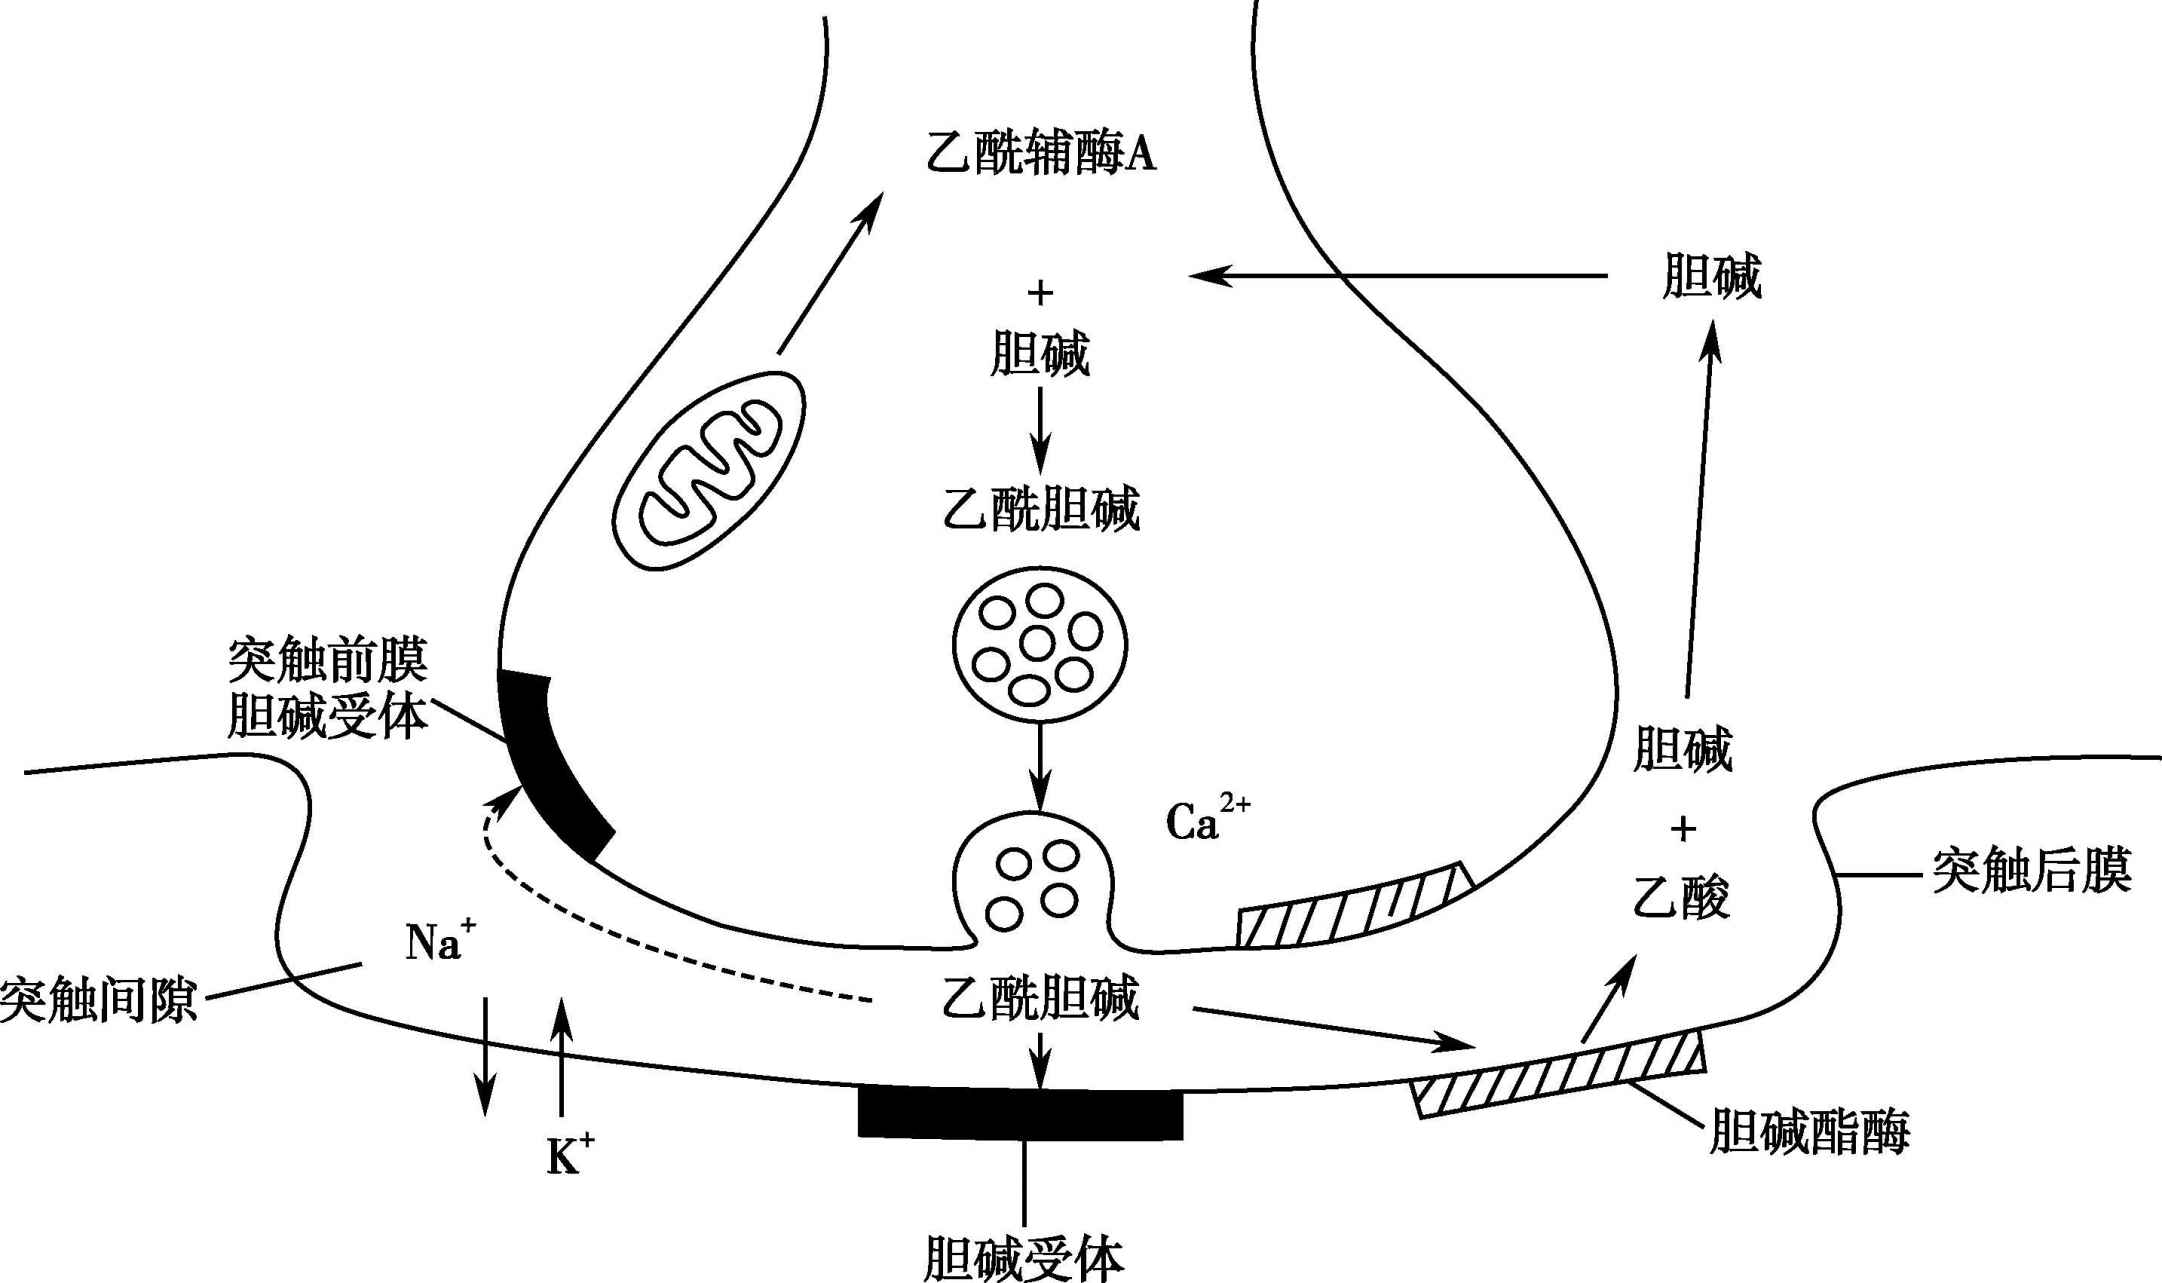
\includegraphics[width=4.77083in,height=2.83333in]{./images/Image00198.jpg}
 \captionsetup{justification=centering}
 \caption{胆碱能神经元突触传递过程示意图}
 \label{fig55-1}
  \end{figure} 

\hypertarget{text00139.htmlux5cux23CHP5-3-1-1-1}{}
(一) 乙酰胆碱的合成、贮存、释放和失活

乙酰胆碱是胆碱能神经末梢释放的递质。胆碱能神经包括:①全部副交感神经节后纤维;②极少数交感神经节后纤维,如支配汗腺分泌的神经和骨骼肌的血管舒张的神经;③全部副交感和交感神经的节前纤维;④运动神经。①、②所支配的效应器细胞膜上的受体是M-胆碱受体(M-AChR),③所支配的神经节细胞膜上的受体是N\textsubscript{1}
-胆碱受体(N\textsubscript{1}
-AChR),④所支配的骨骼肌细胞上的受体是N\textsubscript{2}
-胆碱受体(N\textsubscript{2}
-AChR)。在中枢神经系统有M-AChR和N-AChR,因此也有递质ACh存在。胆碱能神经末梢与效应器接头的传递步骤见图\ref{fig55-2}。

\paragraph{ACh的合成}

合成ACh的前体物为乙酰辅酶A
(AcCoA)与胆碱(choline,Ch)。乙酰辅酶A主要在线粒体中由丙酮酸、脂肪酸生成,而胆碱来自食物(磷脂酰胆碱)或由甘氨酸、丝氨酸在蛋氨酸参加下于肝内合成再由血液供给神经组织。人体血浆内的胆碱浓度约为4.4ng/ml。胆碱通过被动与主动运输机制透过神经膜,如果这种运输过程破坏,则ACh的合成将受阻碍。ACh绝大部分在胆碱神经末稍胞浆内由乙酰辅酶A(AcCoA)与胆碱(Ch)在胆碱乙酰基转移酶(ChAT)的催化下合成。

平时胆碱的来源除上述途径外,还来源于突触前膜(神经末梢)释放的ACh被乙酸胆碱酯酶(AChE)水解后的产物(胆碱)。用标记的胆碱实验证明,约50\%的胆碱被再利用于合成ACh。合成ACh最多的部位是外周胆碱能神经末梢(每小时每克组织2200~5000ng
ACh)。部分ACh可在神经元胞体与轴突内合成,然后携带到末梢。ACh的合成是一种自我调节的过程,据测定,在浓度0.01mol/L时即开始发生抑制过程,使囊泡内的ACh浓度不至过高。这也就是ACh的合成有自我抑制机制(自我保护或自控作用)。

\paragraph{ACh的贮存}

合成的ACh贮存于突触囊泡中,并与特殊的蛋白质结合,此复合物约占囊泡容量的20\%。在囊泡中ACh的浓度可达0.11~0.15mol/L。大部分囊泡是小而无颗粒的小泡,其直径为30~60nm(300~600Å)。一1.ACh生物合成:胆碱(Choline)被吸收进入神经末梢内和乙酰辅酶A(Acety1
CoA)相互作用形成ACh;2.ACh贮存:ACh被贮存于囊泡直至达到一个神经冲动;3.ACh释放:神经末梢的动作电位使囊泡接近突触前膜和释放ACh;4.ACh效应:ACh作用于效应器官的受体而引起效应;5.ACh失活:ACh在突触间隙被乙酰胆碱酯酶(AChE)水解为乙酸与胆碱,胆碱又可被再吸收利用般认为囊泡在神经元胞体形成,然后沿轴浆运输到末梢靠近突触前膜处,一个囊泡内约含有1000~50
000个ACh分子。突触囊泡生存的平均时间约为3周,在此时间内每个囊泡可多次消耗并重新充满递质(ACh)。

\begin{figure}[!htbp]
 \centering
 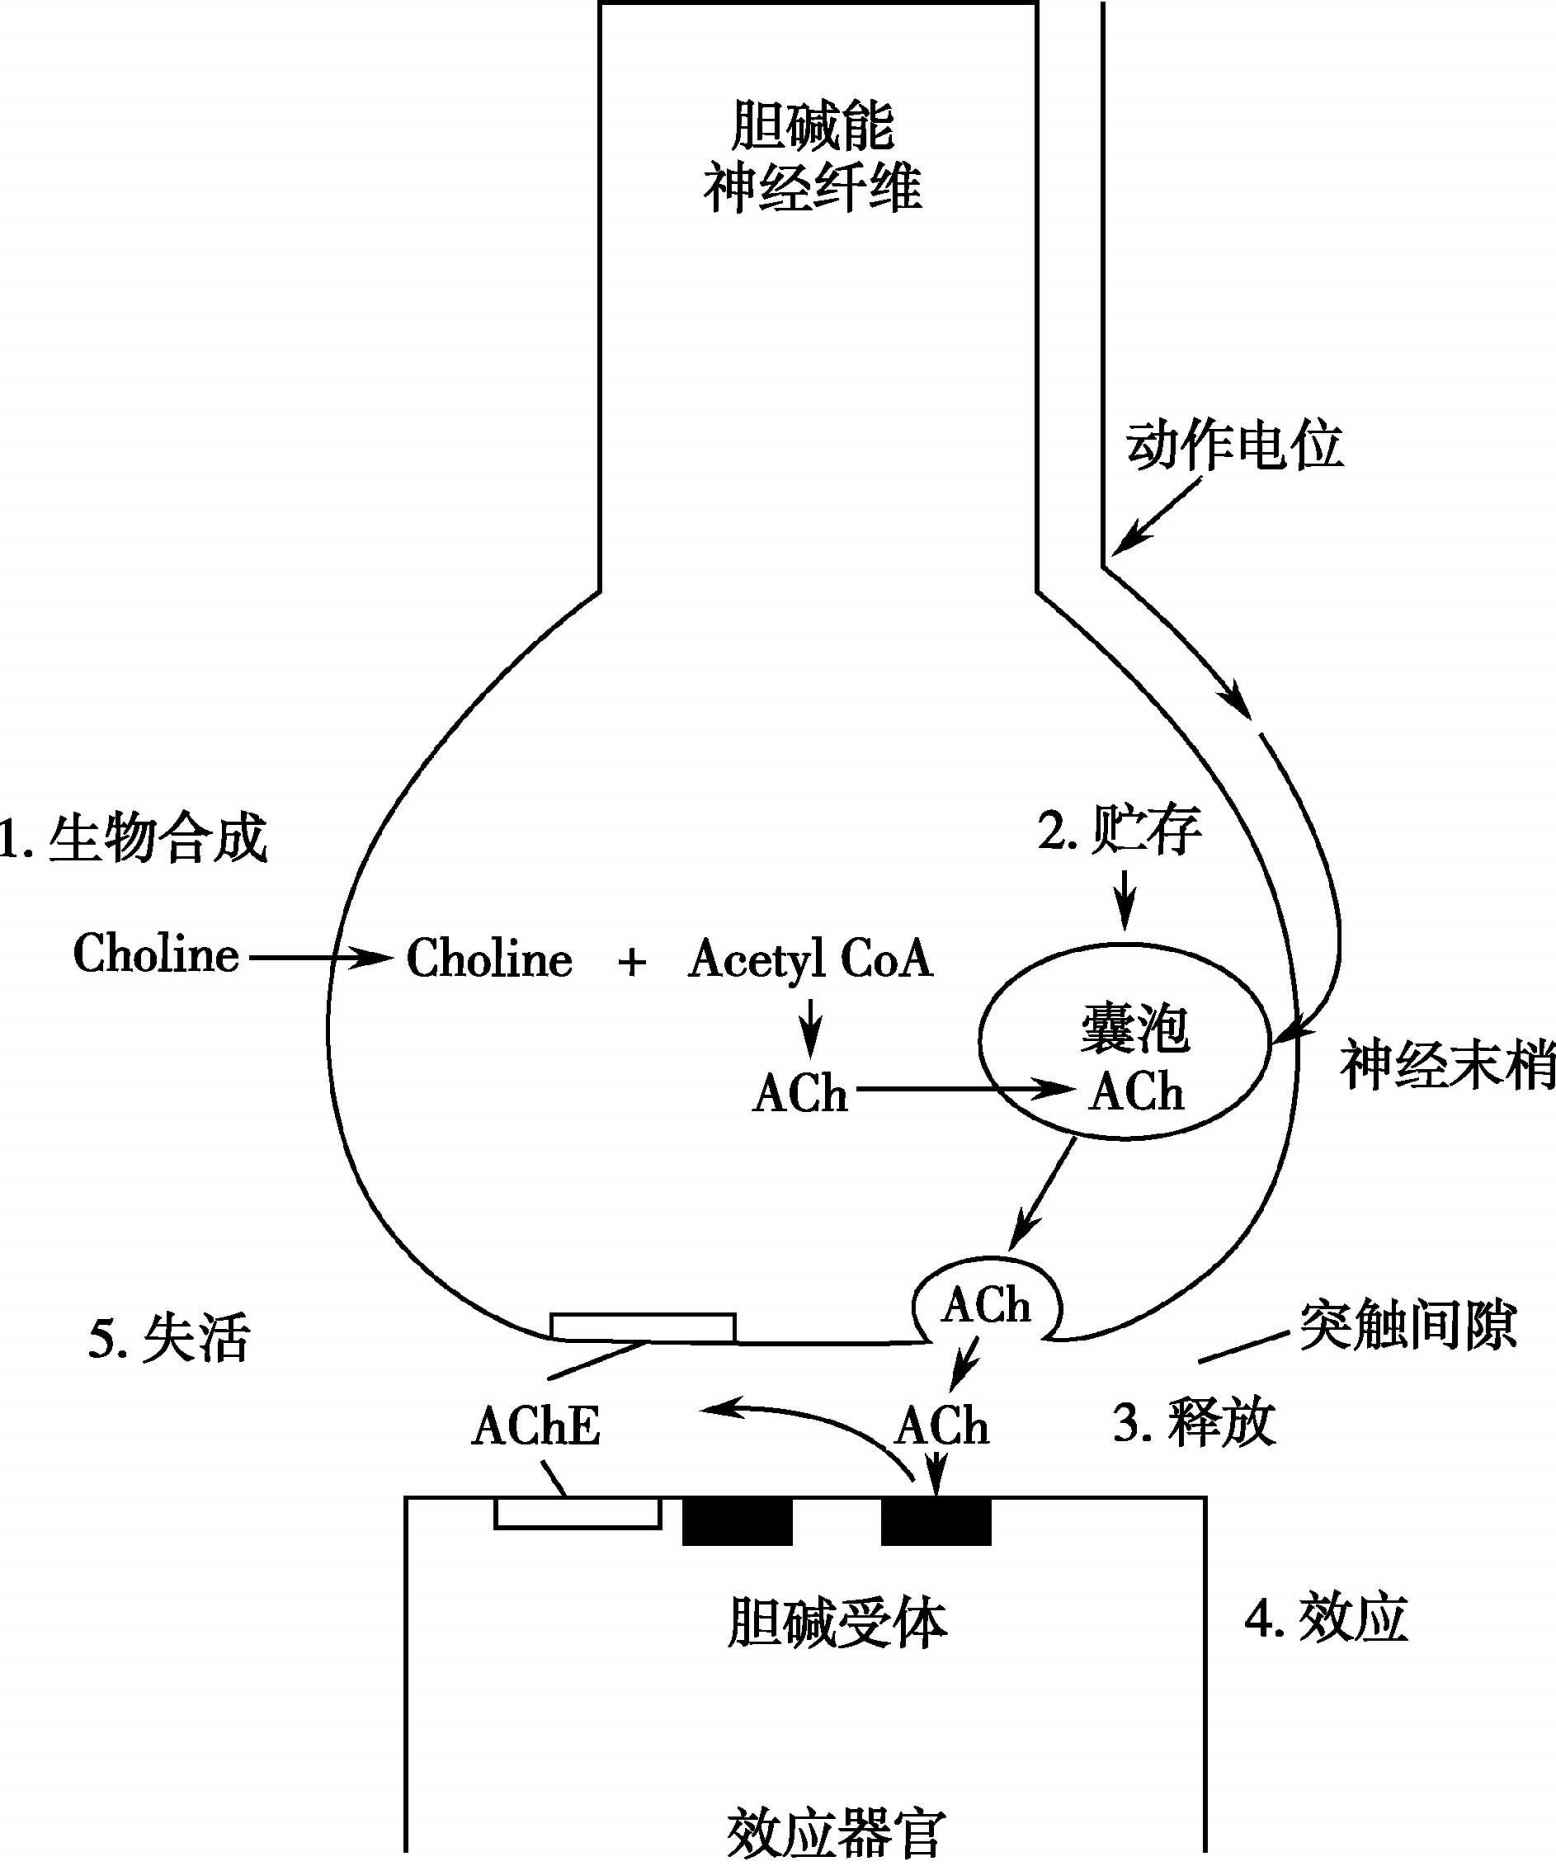
\includegraphics[width=3.13542in,height=3.76042in]{./images/Image00199.jpg}
 \captionsetup{justification=centering}
 \caption{胆碱能神经末梢与效应器官接头的传递步骤示意图}
 \label{fig55-2}
  \end{figure} 

\paragraph{ACh的释放}

ACh是按量子为单位释放的,几千个ACh分子作为一个量子单位同步释放产生一个微终板电位。由数百个微终板电位集合起来形成终板电位。平时神经末梢自发而经常地释放ACh,每分钟约放出0.15~0.5ng递质。在释放过程中,囊泡经过特殊的管道达突触前膜,囊泡膜与之融合而囊泡破裂,递质倾出于突触间隙;随后囊泡膜又脱离前膜并重新补充递质。胆碱能神经纤维末梢或神经元由突触前膜M\textsubscript{2}
受体(自身受体)通过负反馈调控ACh的释放。

\paragraph{ACh与受体的结合}

释放的ACh作用于接头或突触后膜上的胆碱能受体,引起后膜Na\textsuperscript{+}
、K\textsuperscript{+} 等离子通透性的改变,Ca\textsuperscript{2+}
的转移,腺苷酸环化酶系统的激活等,从而引起生理效应。胆碱能受体分为毒蕈型胆碱能受体(M-AChR)和烟碱型胆碱能受体(N-AChR),前者兴奋时发生的反应与毒蕈碱的作用相似,后者兴奋时发生的反应与烟碱相似。胆碱能受体是磷脂蛋白质,ACh与受体结合引起蛋白质构型的改变而离子通道开放,Na\textsuperscript{+}
、K\textsuperscript{+}
的通透性改变。ACh与膜上受体的结合,受乙酰胆碱酯酶(AChE)的调节。ACh被AChE水解后,后膜通道又关闭而恢复原先的状态,从而阻止递质(ACh)在时间上继续发挥作用。

\paragraph{ACh的失活}

在突触后膜与前膜上均分布有乙酰胆碱酯酶(AChE),一次神经冲动释放到突触间隙的ACh在数毫秒内迅速地被AChE水解成胆碱与醋酸(乙酸)而失活,胆碱可被突触前膜重吸收利用,部分弥散至周围体液与血液。据估计突触前膜与突触后膜的AChE水解1分子ACh约需15毫秒时间。此外,使ACh失活的途径可能还有ACh与其他结构的结合,扩散失活以及被非特异性的胆碱酯酶(ChE)所分解,但AChE水解ACh是主要失活方式。

\hypertarget{text00139.htmlux5cux23CHP5-3-1-1-2}{}
(二) 胆碱酯酶的生理功能

\paragraph{胆碱酯酶的分类和分布}

胆碱酯酶(以下简称ChE)是一类能催化水解胆碱酯并能被毒扁豆碱抑制的具有不同专一性的水解酶。根据它催化水解ACh的速度快慢,可将体内的ChE分为真性ChE(AChE)和假性ChE(BChE)。真性ChE对胆碱酯的水解速度依次为乙酰胆碱>丙酰胆碱>丁酰胆碱,它对丁酰胆碱的水解速度很低,甚至是零。假性ChE则相反,其顺序依次为丁酰胆碱>丙酰胆碱>乙酰胆碱。此外,真性ChE还能被高浓度的ACh所抑制,即所谓底物或基质抑制效应;而假性ChE无此特点。

真性ChE存在于神经末梢与神经元突触前、后膜和红细胞,其生理作用是催化水解神经末梢释放的ACh,控制其作用,维持正常胆碱能神经活动。假性ChE主要存在于血浆、肝、肺和心肌等部位,其生理作用至今尚不清楚(表\ref{tab55-1})。真性ChE(AChE)在神经元胞体中合成,可区分为细胞质内酶(膜内酶)和细胞膜外表面酶(膜外酶)。只有位于细胞(突触)膜外表面的AChE才能接触神经末梢释放的ACh和又最接近ACh作用的受体,故这些部位的AChE也称为功能性酶。而位于细胞质内的AChE是合成后尚未输送到膜外面的膜内酶,故也称为贮存AChE。

\begin{table}[htbp]
\centering
\caption{体内不同部位的 ChE性能与来源}
\label{tab55-1}
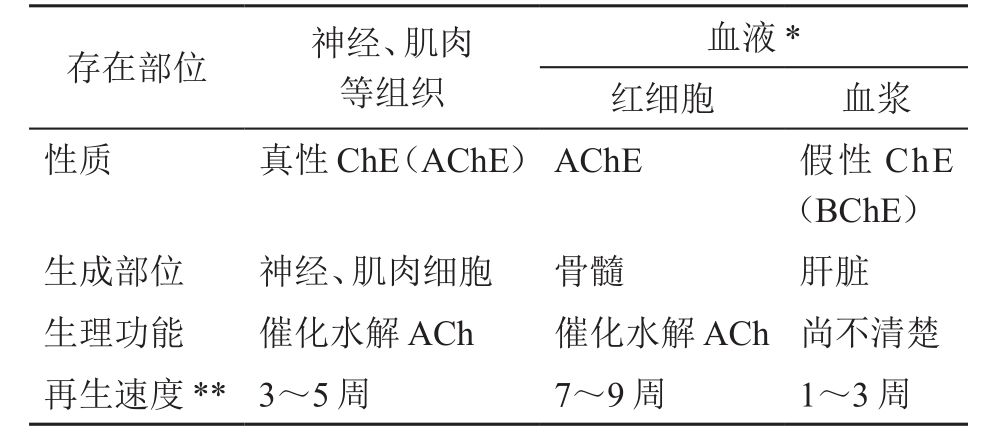
\includegraphics[width=3.29167in,height=1.4375in]{./images/Image00200.jpg}
\end{table}

*血液ChE总活性中,大约红细胞占60\%~80\%,血浆占20\%~40\%;**再生速度指中、重度中毒中毒酶“老化”后,ChE再生接近正常水平大约所需的时间

\paragraph{AChE催化水解ACh的原理}

AChE是一种含糖的蛋白质,分子量为23万~26万道尔顿。它的活性部位(活力中心)包括相距0.5nm两个部位,即负矩部位(阴离子部位)和酯解部位。酯解部位中有3个功能基团,即酸性基团、酰化基团及碱性基团。负矩部位为二羧酸(门冬氨酸或谷氨酸)的游离羧基,其周围还有疏水区。

当ACh靠近AChE的活性表面时,ACh的三甲铵阳离子(带正电)与AChE的负矩部位(带负电)依靠静电引力形成离子键而结合;使ACh固定在最有利于酯解部位水解ACh的位置。

AChE对ACh水解的催化过程主要在酯解部位进行。在酯解部位的酸基和碱基协助下,ACh的乙酰基上的碳原子与AChE丝氨酸上的氧原子形成共价键结合;同时ACh的酯键断裂,乙酰基与AChE结合,形成乙酰化酶。随后,ACh的胆碱从负矩部位脱落。最后,乙酰化酶上的乙酰基很快从酶的酯解部位自动脱落,重新形成自由酶,即AChE恢复到与ACh结合之前的状态,又可重新催化水解ACh(图\ref{fig55-3})。

\hypertarget{text00139.htmlux5cux23CHP5-3-1-1-3}{}
(三) 有机磷农药对胆碱酯酶的抑制作用

有机磷农药与
AChE的作用原理和ACh与AChE的结合方式基本上相似。在AChE酯解部位的酸基和碱基协助下,有机磷农药的磷原子与AChE酯解部位的丝氨酸上的氧原子形成共价键结合;同时酯键断裂,磷酰基与AChE结合形成磷酰化酶(图\ref{fig55-4})。

有机磷农药和ACh分别与AChE的结合方式虽然基本相似,但由于前者形成磷酰化酶(中毒酶),后者形成乙酰化酶,而导致了截然不同的结果。乙酰化酶如上所述,其乙酰基能在极短时间内自动脱落,乙酰化酶重新恢复为自由酶,继续行使正常功能(催化ACh水解)。而磷酰化酶(中毒酶)的脱磷酰基反应速度极慢,有些情况下接近零,根本不能重新恢复为自由酶;因此,这个AChE分子失去活性而不能再催化水解ACh,一般将其失去活性的磷酰化酶称为中毒酶。

\hypertarget{text00139.htmlux5cux23CHP5-3-1-1-4}{}
(四) 中毒酶(磷酰化酶)的转归

中毒酶(磷酰化酶)的形成并不是反应的终结,它的自然转归可以向两个方向转化。一个方向是整个磷酰基脱落,ChE自动恢复其水解ACh活性,称为自动活化反应;另一个方向是磷酰基的部分基团脱落(脱烷基),ChE失去活性即老化反应。当上述两个转化的反应尚未发生时,如果应用适当的药物(复能剂)促进中毒酶的磷酰基脱落而重新恢复为自由酶,称为重活化反应。因此,中毒酶形成后的命运现在已知有三个,前两个是自然转归,后一个是用人工手段造成的重要转归,也是有机磷农药中毒救治的根本措施。

\begin{figure}[!htbp]
 \centering
 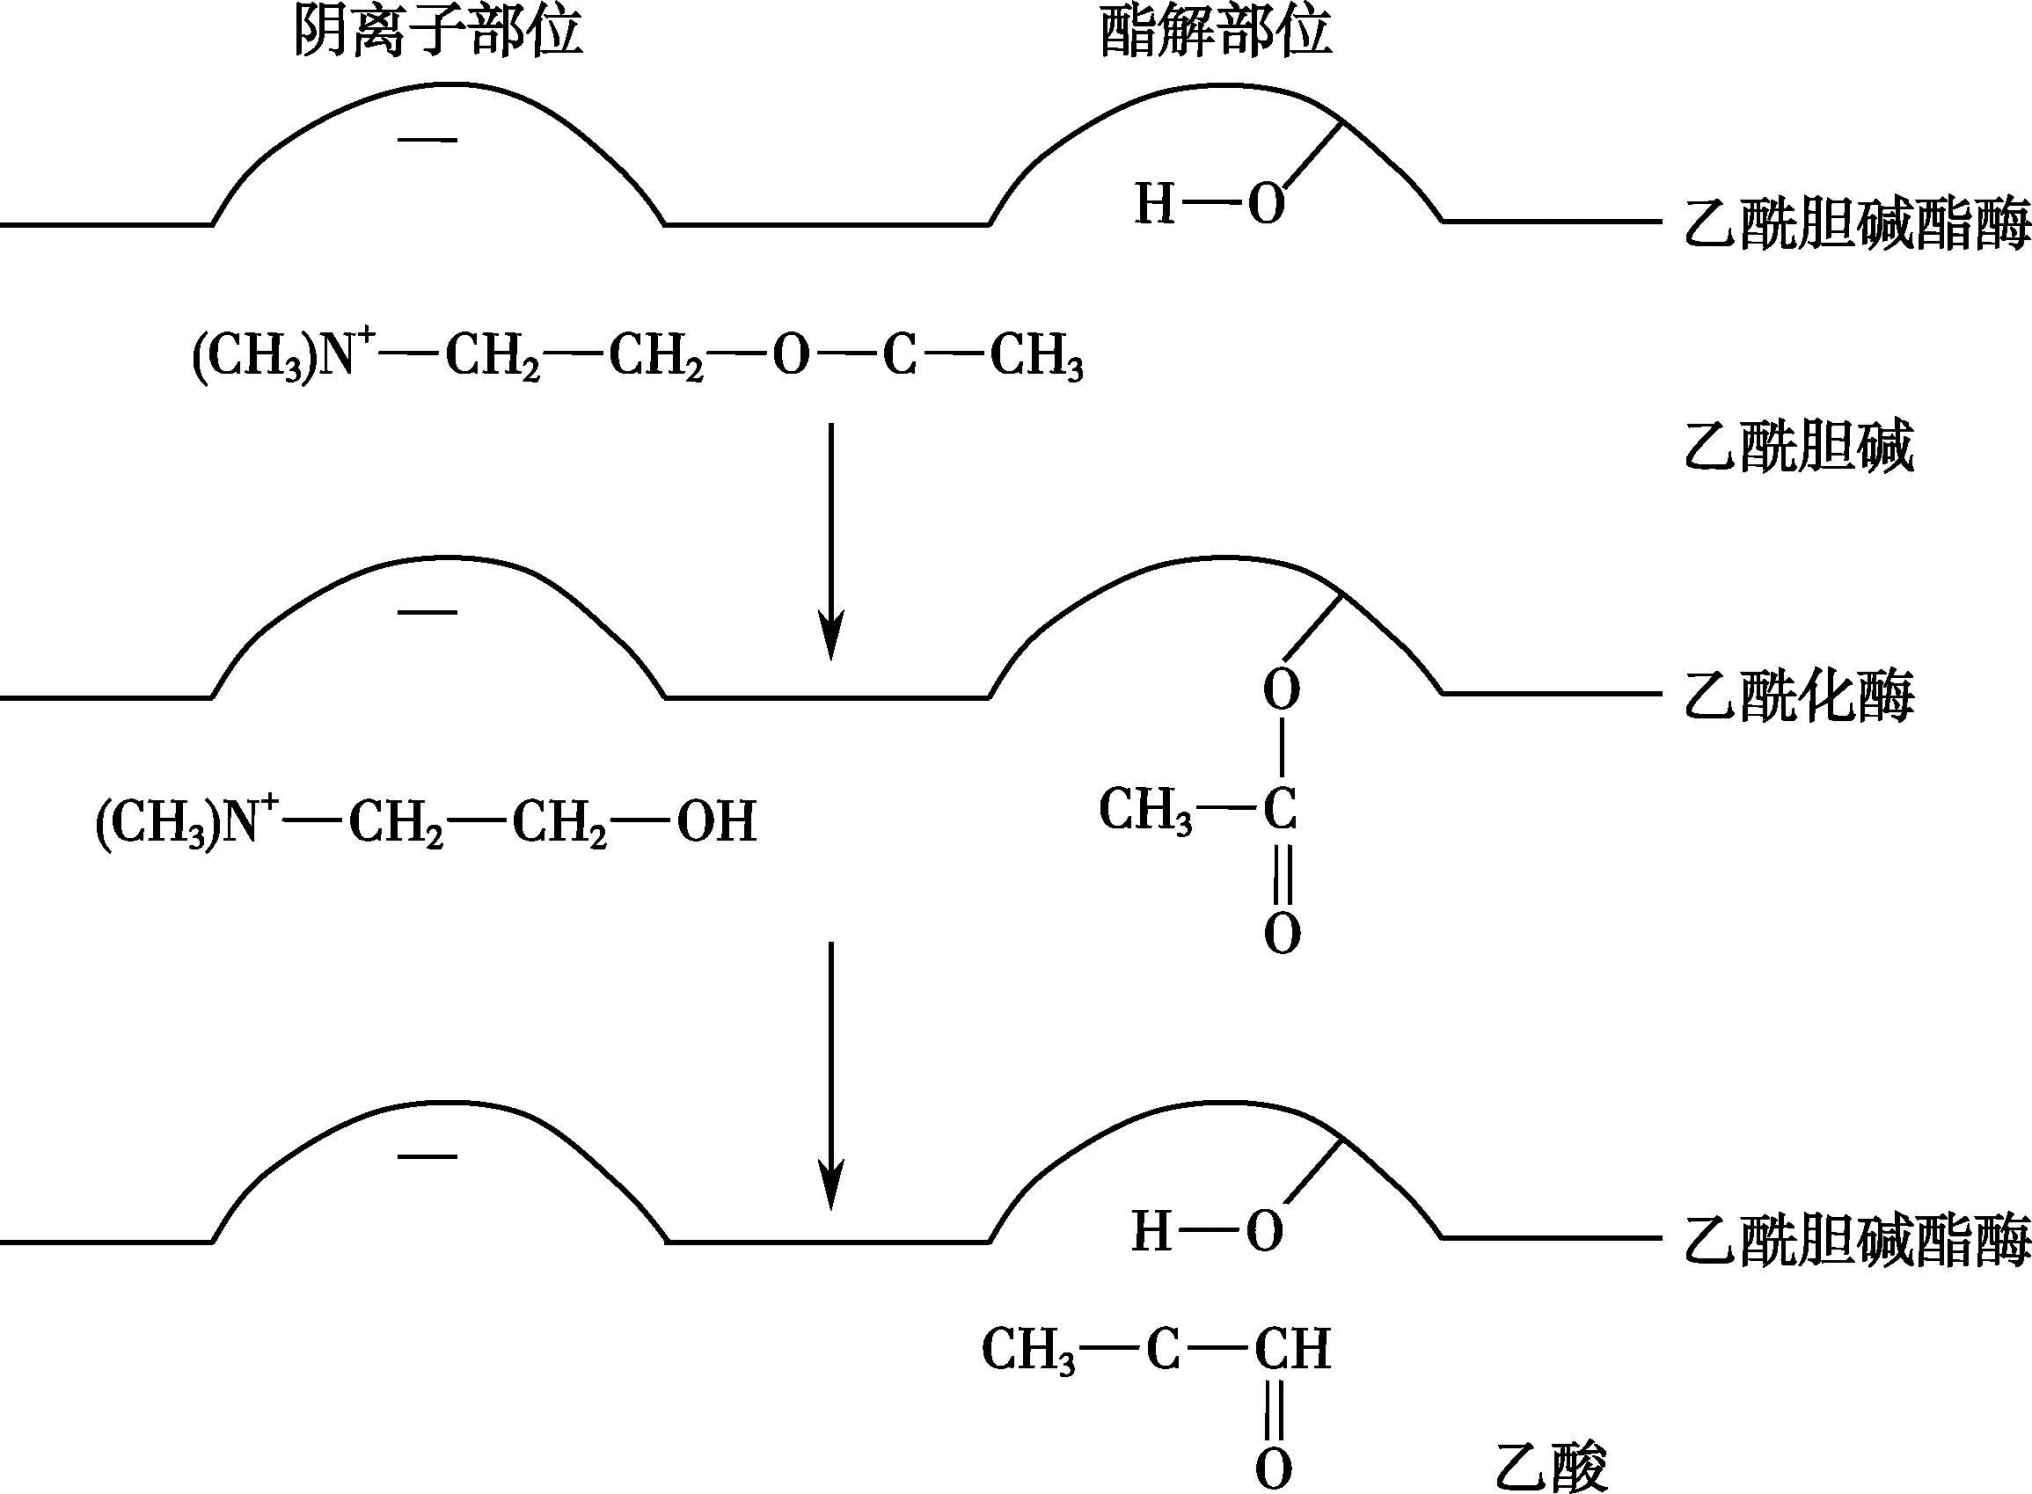
\includegraphics[width=3.84375in,height=2.83333in]{./images/Image00201.jpg}
 \captionsetup{justification=centering}
 \caption{乙酰胆碱酯酶催化水解乙酰胆碱示意图}
 \label{fig55-3}
  \end{figure} 

\begin{figure}[!htbp]
 \centering
 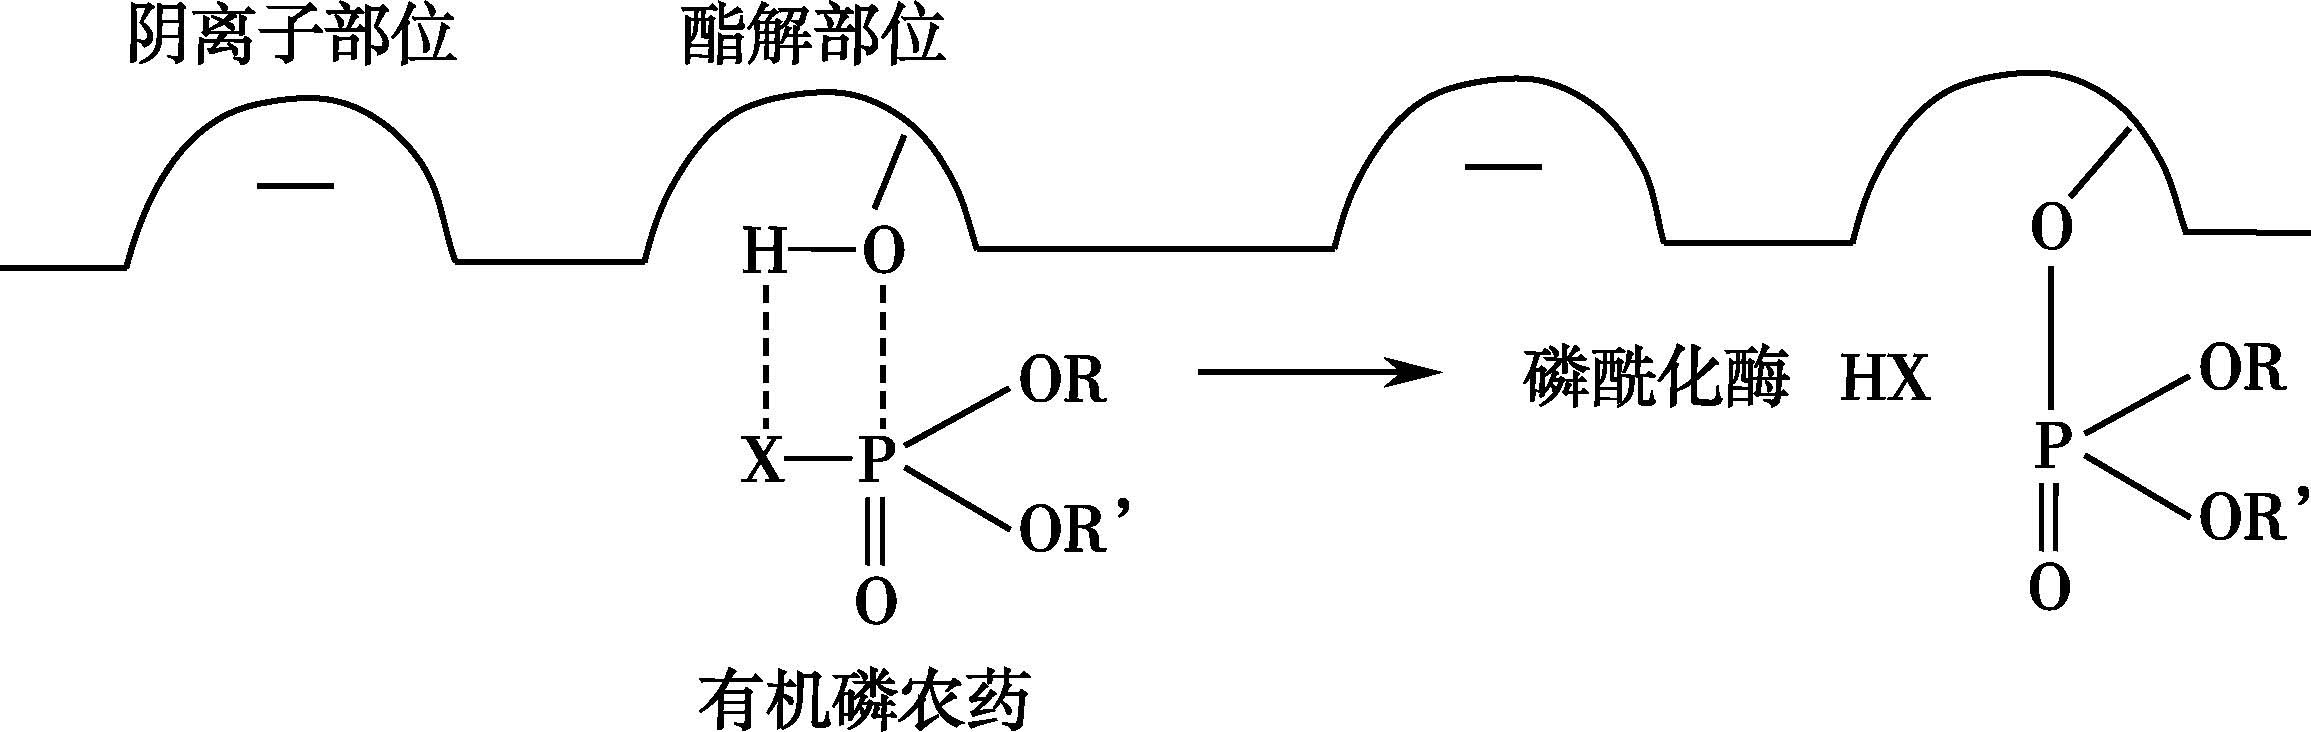
\includegraphics[width=3.84375in,height=1.21875in]{./images/Image00202.jpg}
 \captionsetup{justification=centering}
 \caption{有机磷农药与乙酰胆碱酯酶 AChE结合示意图}
 \label{fig55-4}
  \end{figure} 

\paragraph{自动活化}

自动活化就是中毒酶磷酰基自动脱落而成为自由酶。如前所述,这种脱磷酰基反应速度极慢,有的中毒酶基本上观察不到脱磷酰基反应,如梭曼中毒酶;有些中毒酶虽能观察到自动活化,但需数小时或数十小时。因此,有机磷农药中毒后形成的中毒酶,如仅依靠自动活化,而不给予适当药物促进重活化,不但病程常常较长,而且易出现死亡。

\paragraph{老化}

中毒酶随着时间的进程或早或晚地进一步发生结构上的变化,其磷酰基的部分基团脱落即脱烷基反应,这种脱烷基反应称为老化。中毒酶老化后,不能再发生脱磷酰基反应或重活化反应,其水解ACh的活性不能再恢复。因而,当有机磷农药中毒后,应尽早给予适当的药物,促进中毒酶重活化,避免老化;否则,将为治疗带来较大困难,或易出现死亡。

中毒酶的老化速度快慢与其导致中毒的有机磷化合物的结构有关,主要取决于磷酰基上烷氧基团的结构,即磷酰化酶的内部因素;而机体中的环境只是变化的条件,是第二因素。

\paragraph{重活化}

当中毒酶的磷酰基尚未自动脱落而自动活化,又未进一步部分基团脱落(脱烷基)而老化时,应用适当的药物能大大加快脱磷酰基反应的速度,这种药物促进的脱磷酰基反应称为重活化反应,其药物称为重活化剂或复能剂。一旦中毒酶的磷酰基脱落重新恢复为自由酶后,又可继续行使催化ACh水解的正常功能,一切中毒症状将消失。因此,在救治有机磷农药中毒患者时,应在中毒酶未老化之前尽早给予重活化剂,这是最根本的措施,故也可以把重活化剂称为特效解毒药。但在中毒酶尚未恢复为自由酶时,过多的ACh引起的中毒症状(胆碱能危象)尚需应用抗胆碱药物治疗,这也是重要的治标保本的措施。

中毒酶可向三个方向转归是就中毒酶分子群体而言的,对于某一个中毒酶分子来说,则只有一种转归的可能。一种中毒酶主要朝哪个方向转归,其自然转归取决于磷酰基上烷氧基团的结构,即中毒酶的内部因素。但中毒酶是否朝重活化方向转归(人工转归),则主要取决于应用重活化剂的早晚和剂量,如尽早足量用药,一般中毒酶或多或少均可朝重活化方向转归。因此,中毒酶是否朝重活化方向转归,在很大程度上取决于人为的因素。当由于主观或客观原因导致中毒酶老化后,则必须给予适量的抗胆碱药物维持轻度“阿托品化”,直至ChE恢复(新生)到60\%以上。而目前用于维持“阿托品化”最理想的药物为盐酸戊乙奎醚(长托宁),它不但持续时间长,而且毒副作用小(详见后述)。

\subsection{诊断}

\subsubsection{有机磷农药接触史}

有机磷农药接触史是确诊有机磷农药中毒的主要依据,特别是对无典型中毒症状或体征者更为重要。凡近期(一般指12小时内)参加过有机磷农药生产、包装、搬运、保管、配制、喷洒或使用过有机磷农药,接触过有机磷农药器械或被农药污染的器具,吃过农药污染的粮食、食品或近期喷洒过农药的水果、蔬菜,穿过被农药污染的衣服,在存放农药的屋内停留过较长时间等,都属于有农药接触史。当中毒者及其家属不能明确提供上述接触史时,医生应根据患者的发病症状及其特点仔细地询问有关病史。对口服或误服农药中毒者,则应详细了解服用农药的种类、剂型和剂量,最好能得到服用农药的农药瓶或容器及其剩余的农药,以免有误。特别是对一些自服中毒者更应如此,不可仅根据患者或家属所述而定;医生应根据患者的发病过程及其特点综合分析判断。

\subsubsection{临床表现特点}

有机磷农药中毒后可出现一系列中毒症状和体征(表\ref{tab55-2})。经皮肤吸收中毒,一般在接触2~6小时后发病,口服中毒在10分钟~2小时内出现症状。一旦中毒症状(急性胆碱能危象)出现后,病情迅速发展。其典型症状和体征主要有:流涎、大汗、瞳孔缩小和肌颤(肉跳)。一般当出现上述症状或体征和有农药接触史,可诊断为AOPP;如四个症状或体征中仅出现三个,也应考虑为AOPP。

\paragraph{急性胆碱能危象(acute cholinergic crisis)}

表现为:

\hypertarget{text00139.htmlux5cux23CHP5-3-1-2-2-1-1}{}
(1) 毒蕈碱样症状(muscarinic signs):

又称M样症状,主要是副交感神经末梢过度兴奋,产生类似毒蕈碱样作用,表现为平滑肌痉挛和腺体分泌增加。先有恶心、呕吐、腹痛、多汗,尚有流泪、流涕、流涎、腹泻、尿频、大小便失禁、心跳减慢和瞳孔缩小;支气管痉挛和分泌物增加、咳嗽、气促,严重者出现肺水肿。

\hypertarget{text00139.htmlux5cux23CHP5-3-1-2-2-1-2}{}
(2) 烟碱样症状(nicotinic signs):

又称N样症状,ACh在横纹肌神经肌肉接头处过多蓄积和刺激,使面、眼睑、舌、四肢和全身横纹肌发生肌纤维颤动,甚至全身肌肉强直性痉挛、全身紧缩和压迫感,而后发生肌力减退和瘫痪。呼吸肌麻痹引起周围性呼吸衰竭。交感神经节受ACh刺激,其节后交感神经纤维末梢释放儿茶酚胺,表现血压升高和心律失常。

\hypertarget{text00139.htmlux5cux23CHP5-3-1-2-2-1-3}{}
(3) 中枢神经系统症状:

过多ACh刺激所致。表现头晕、头痛、疲乏、共济失调、烦躁不安、谵妄、抽搐和昏迷。有的发生呼吸、循环衰竭死亡。

\hypertarget{text00139.htmlux5cux23CHP5-3-1-2-2-1-4}{}
(4) 局部损害:

有些有机磷农药接触皮肤后发生过敏性皮炎、皮肤水疱或剥脱性皮炎;污染眼部时,出现结膜充血和瞳孔缩小。

\paragraph{中间型综合征(intermediate syndrome)}

多发生于重度AOPP(甲胺磷、乐果、敌敌畏、久效磷等)中毒后24~96小时,在胆碱能危象和迟发性多发性神经病之间,故称中间型综合征,但并非每个中毒者均发生。发病时胆碱能危象多已控制,表现以肌无力最为突出。涉及颈肌、肢体近端肌、脑神经Ⅲ~Ⅶ和Ⅹ所支配的肌肉,重者累及呼吸肌。表现为:抬头困难、肩外展及髋曲困难;眼外展及眼球活动受限,眼睑下垂,睁眼困难,复视;颜面肌、咀嚼肌无力、声音嘶哑和吞咽困难;呼吸肌麻痹则有呼吸困难、频率减慢、胸廓运动幅度逐渐变浅,进行性缺氧致意识障碍、昏迷以至死亡。ChE活性明显低于正常。一般维持2~20天,个别可长达1个月。其发病机制与ChE长期受抑制,影响神经肌肉接头处突触后功能有关。

\paragraph{迟发性多发性神经病(delayed polyneuropathy)}

\begin{table}[htbp]
\centering
\caption{有机磷农药中毒的症状和体征}
\label{tab55-2}
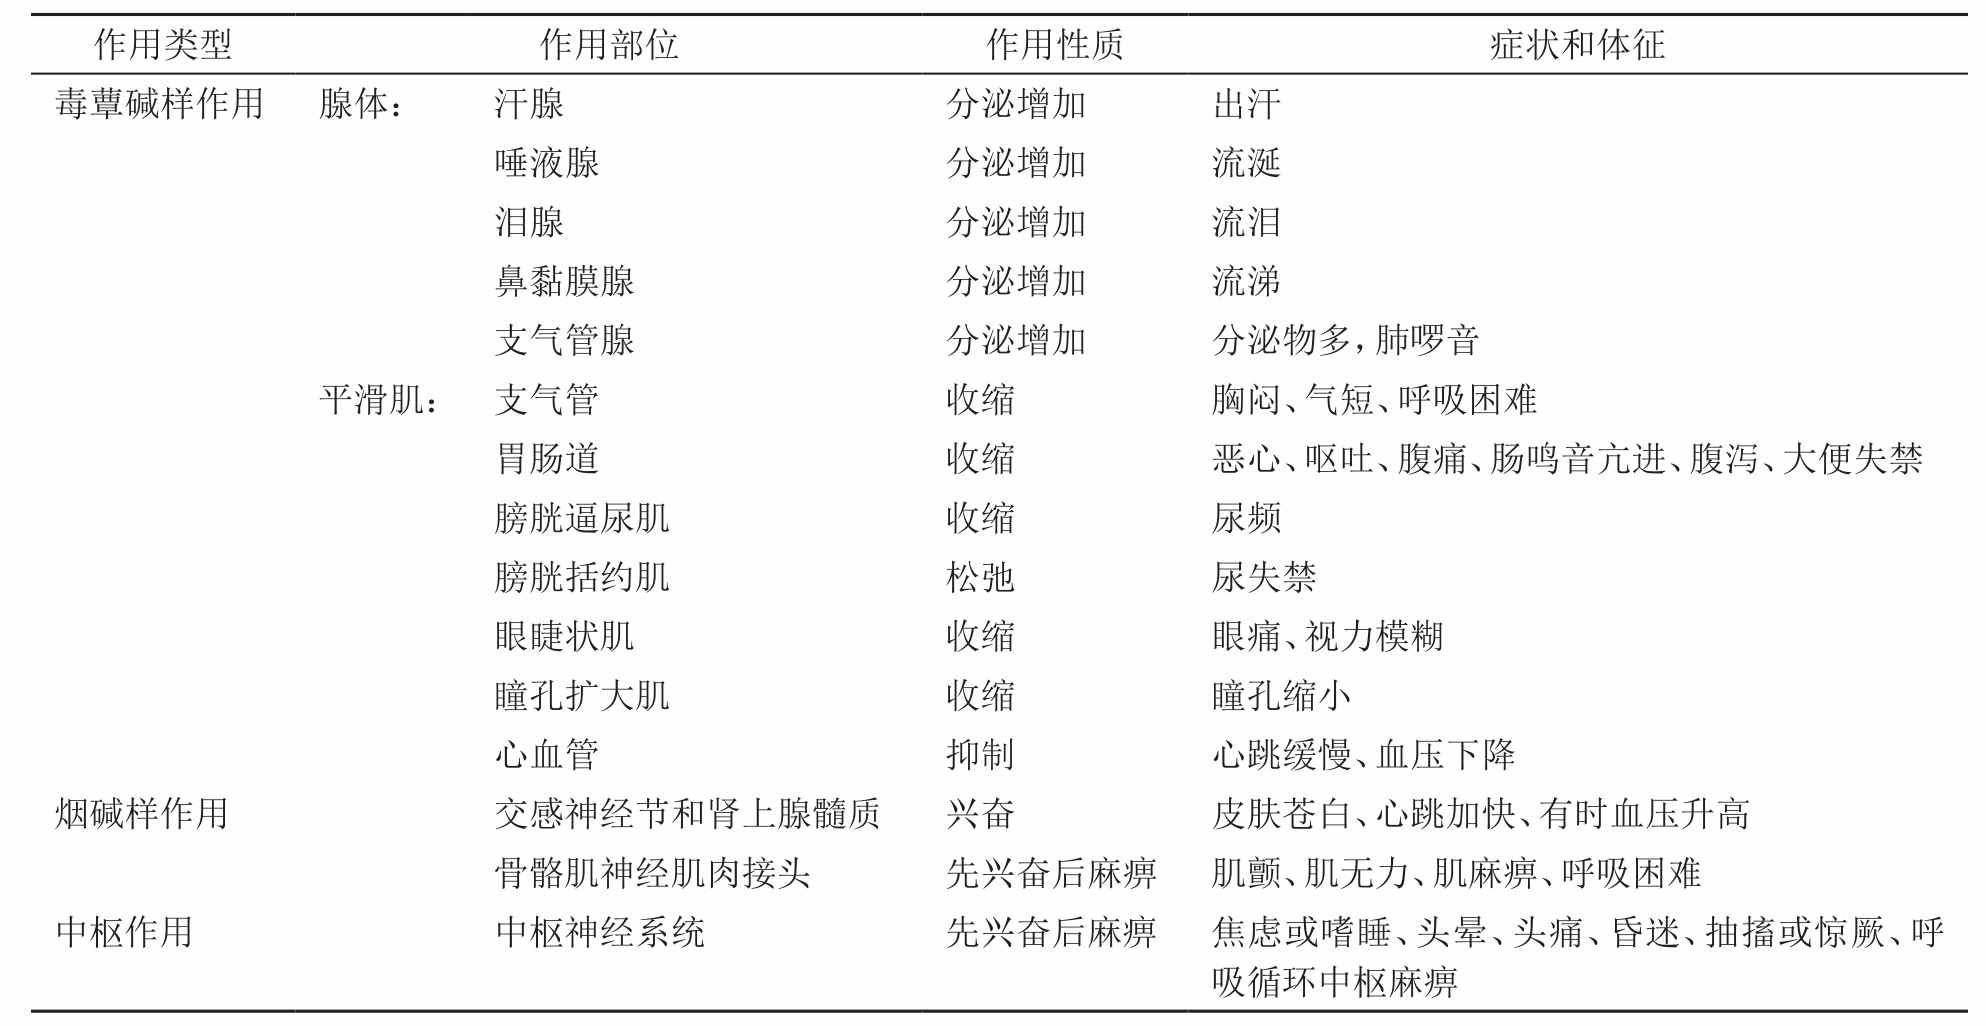
\includegraphics[width=6.61458in,height=3.41667in]{./images/Image00203.jpg}
\end{table}

AOPP患者症状消失后2~3周出现迟发性神经损害,表现感觉、运动型多发性神经病变,主要累及肢体末端,发生下肢瘫痪、四肢肌肉萎缩等。全血ChE活性正常,神经-肌电图检查提示神经源性损害。目前认为此种病变不是ChE受抑制引起,可能是由于有机磷农药抑制神经靶酯酶(neuropathy
target
esterase,NTE)使其老化所致。多发生于甲胺磷、敌敌畏、乐果和敌百虫等有机磷农药重、中度中毒的患者。

\subsubsection{实验室检查}

\paragraph{血胆碱酯酶活性测定}

红细胞的ChE为真性ChE
(AChE);血浆ChE为假性ChE(BChE),不能水解ACh,主要来自肝脏,受肝功能的影响较大;故全血ChE(总活性中红细胞占60\%~80\%,血浆占20\%~40\%)和红细胞的AChE活性能较好的反映神经肌肉等组织中的AChE活性水平。所以一般测定全血胆碱酯酶活性(ChE),也可测定红细胞AChE活性。ChE活性测定不仅是诊断有机磷农药中毒的一项可靠检查,而且是判断中毒程度、指导用药、观察疗效和判断预后的重要参考指标。急性有机磷农药中毒程度和临床表现与ChE活性有相对平行关系。一般全血ChE活性下降到70\%以下时,可出现中毒症状;下降到30\%~40\%时,可出现明显中毒症状。但如经反复多次吸入有机磷农药蒸汽或较长时间接触有机磷农药者,其ChE活性与中毒程度和临床表现无平行关系。有的中毒者ChE活性下降至50\%或更低,可不出现明显中毒症状,这种情况多见于生产有机磷农药厂的工人和较长时间喷洒或接触有机磷农药的农民。

\paragraph{有机磷农药的鉴定}

当中毒者使用或服用的农药或毒物种类不清时,可对其剩余物进行鉴定。

\paragraph{尿中有机磷农药分解产物测定}

如对硫磷中毒尿中测到对硝基酚,敌百虫中毒尿中三氯乙醇增加。

\subsubsection{急性中毒程度分级}

\paragraph{轻度中毒}

仅有M样症状,全血ChE活力70\%~50\%。

\paragraph{中度中毒}

M样症状加重,出现N样症状,ChE活力50\%~30\%。

\paragraph{重度中毒}

除M、N样症状外,合并肺水肿、抽搐、意识障碍,呼吸肌麻痹和脑水肿,ChE活力<
30\%。

\subsubsection{诊断注意事项}

根据患者有机磷农药接触史、呼出气大蒜味、瞳孔缩小、多汗、肌纤维颤动和意识障碍等,不难诊断。对于不明原因的意识障碍、瞳孔缩小,并伴有肺水肿患者,也应考虑到AOPP,如监测全血ChE活力降低,可确诊。

当轻度中毒患者无上述有机磷农药中毒典型症状和体征时,则主要根据有机磷农药接触史和通过必要的化验检查如胆碱酯酶活性测定来确诊。

在使用农药季节,特别是在夏天,往往易将夏季常见的疾病或非有机磷农药中毒误诊为有机磷农药中毒,或将有机磷农药中毒误诊为急性胃肠炎、食物中毒、中暑、感冒和其他种类农药中毒。故应根据上述有机磷农药中毒诊断主要依据和其他中毒或疾病鉴别。

\paragraph{与夏季常见病相鉴别}

在使用农药季节,夏季常见病中的急性胃肠炎、食物中毒和中暑等,常因出现头晕、头痛、无力、恶心、呕吐和腹泻等症状而易误诊为有机磷农药中毒;如患者同时具有接触有机磷农药史时,其误诊更为常见。因此,常常导致不良后果,甚至有的患者死于阿托品中毒。

上述夏季常见病与有机磷农药中毒的主要鉴别要点,前者一般不出现大汗、瞳孔缩小、肌颤和胆碱酯酶活性下降,而后者可出现上述症状和体征(表\ref{tab55-3})。

\begin{table}[htbp]
\centering
\caption{有机磷农药中毒与夏季常见病的鉴别要点}
\label{tab55-3}
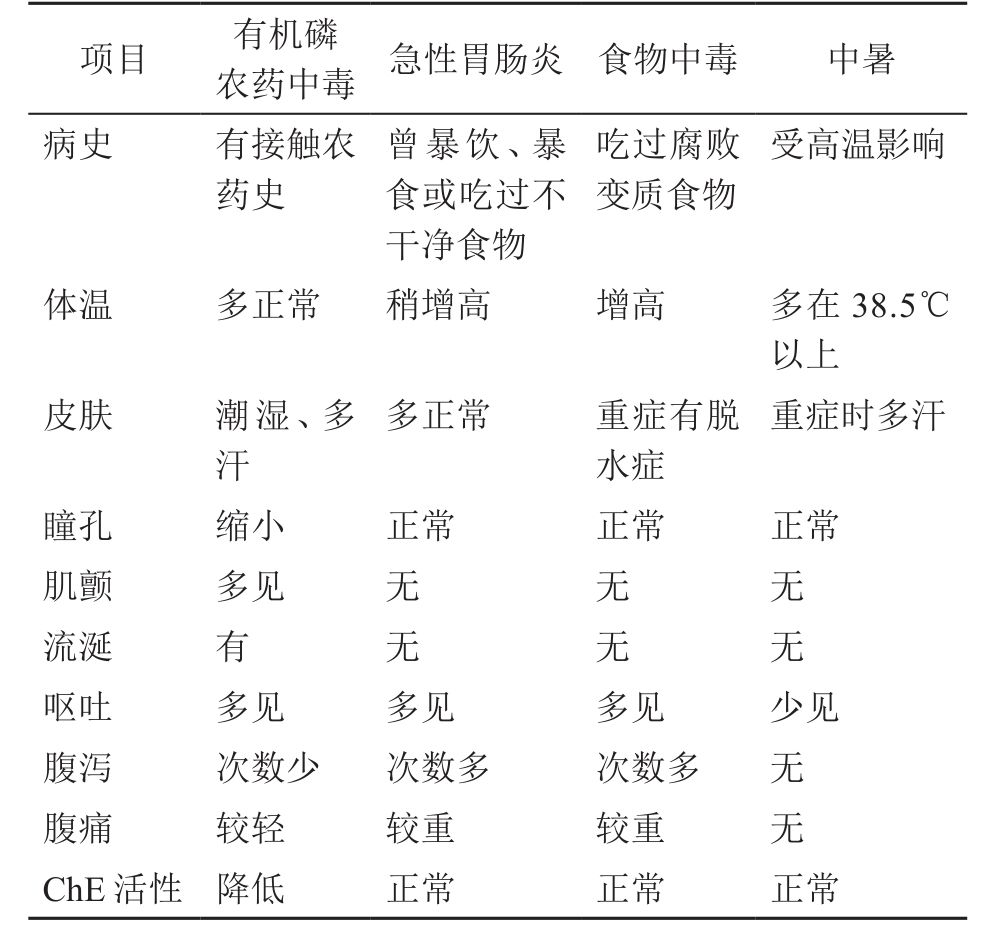
\includegraphics[width=3.32292in,height=3.14583in]{./images/Image00204.jpg}
\end{table}

\paragraph{与其他种类农药中毒相鉴别}

目前除广泛使用有机磷农药外,尚使用氨基甲酸酯类、拟除虫菊酯类和有机氮类等农药。氨基甲酸酯类常见的品种有呋喃丹、西维因、涕灭威等;拟除虫菊酯类常见的品种有溴氢菊酯(敌杀死)、杀灭菊酯(速灭杀丁)等;有机氮类常见的品种有杀虫脒、杀虫双等。这些农药中毒与有机磷农药中毒的主要鉴别要点,在于两者除农药接触史和临床表现不同外,有机磷农药中毒者体表或呕吐物一般有蒜臭味,而前者一般无蒜臭味。详见有关章节。

\subsection{治疗}

AOPP救治原则为:切断毒源,治本为主;标本兼治,以标保本。在急救中必须视当时具体情况或患者的病情,采取先后顺序不同的相应急救措施。

\subsubsection{迅速清除毒物}

立即将中毒者移离染毒环境,彻底清除未被机体吸收进入血的毒物,如脱去污染衣物,用清水或肥皂水彻底清洗染毒的皮肤、指甲下和毛发。眼部污染时,用清水、生理盐水、2\%碳酸氢钠溶液或3\%硼酸溶液冲洗。经口中毒者尽早洗胃,原则是宜用粗胃管反复洗胃,持续引流,即首次洗胃后保留胃管,间隔3~4小时重复洗胃,洗至引出液清澈、无味为止。洗胃液可用清水、2\%碳酸氢钠溶液(敌百虫忌用)或1∶5000高锰酸钾溶液(对硫磷忌用)。洗胃液总量一般需要10L左右。应待病情好转、ChE活力基本恢复正常方可拔掉胃管。洗胃后注入20\%甘露醇250ml或50\%硫酸钠60~100ml导泻。如因喉头水肿或痉挛,不能插入胃管,或饱食后胃管阻塞,可剖腹胃造瘘洗胃。其优点是清洗彻底,缺点是手术创伤,增加感染机会,并可能使毒物污染腹腔。

\subsubsection{特效解毒剂的应用}

在清除毒物过程中,应同时使用胆碱酯酶重活化剂和抗胆碱药治疗。用药原则是:根据病情早期、足量、联合和重复应用解毒药,并且选用合理用药途径及择期停药。

\hypertarget{text00139.htmlux5cux23CHP5-3-1-3-2-1}{}
(一) 胆碱酯酶重活化剂

目前常用的胆碱酯酶重活化剂有碘解磷定(PAM-I,pralidoxime
methiodide)、氯解磷定(PAM-CL,pralidoxime
chloride)、甲磺磷定(P\textsubscript{2}
S)、双复磷(DMO\textsubscript{4} ,LüH\textsubscript{6}
,toxogonin)和双解磷(TMB\textsubscript{4}
,trimedoxime)等,这些药物都是肟类化合物,故又称肟类重活化剂。它们都含有季铵基和肟基{}
两个不同的功能基团,季铵基是一个阳离子头,能与磷酰化ChE(中毒酶)的阴离子部位通过静电引力促使药物靠近中毒酶,使肟基部位与磷酰基接近。肟基和中毒酶的磷原子亲和力较强,结合形成肟类------中毒酶复活物(中间络合物)。然后,磷酰基从中毒酶上脱落下来形成磷酰肟,于是ChE游离出来而恢复其水解ACh的活性。

肟类重活化剂不但能使磷酰化ChE的活性重活化,而且对有机磷农药中毒引起的肌颤、肌无力和肌麻痹有一定的直接对抗作用(抗烟碱样作用);此外,尚有较弱的阿托品样作用(抗毒蕈碱样作用)。

碘解磷定、氯解磷定和甲磺磷定三者的母体结构相同,只是前者为碘甲烷盐,中者为氯甲烷盐,后者为甲磺酸盐;由于碘的分子量较大,有效含肟量相对较小,故1.53g碘解磷定的作用相当于1g氯解磷定的作用。碘解磷定、氯解磷定和甲磺磷定均含一个肟基,比含有二个肟基的双复磷和双解磷的作用弱。

我国目前主要应用氯解磷定(首选)和碘解磷定,美国常用氯解磷定,欧洲一些国家喜欢用双复磷和双解磷,英国主要使用甲磺解磷定;但一般认为这五个药中的首选药是氯解磷定或双复磷。氯解磷定和双复磷不但含肟量高,重活化作用较强,而且毒副作用较小。双解磷的毒副作用较大。碘解磷定不但含肟量低,重活化作用较弱,而且使用不便(只能静脉注射,且溶积较大)和用量较大时副作用较大(表\ref{tab55-4})。因此,目前大多国家早已不使用碘解磷定。

氯解磷定(氯磷定)的首次用量为:轻度中毒0.5~1.0g,中度中毒1.0~2.0g,重度中毒2.0~3.0g,肌肉注射或静脉注射。碘解磷定(解磷定)的剂量按氯解磷定剂量折算,1g氯解磷定相当于1.5g碘解磷定,本品只能静脉应用。碘解磷定的首次用量为:轻度中毒0.4~0.8g,中度中毒0.8~1.2g,重度中毒1.2~1.6g。首次给药要足量,旨在使解毒剂短时间内尽快达到有效血药浓度。应用ChE复能药后,N样症状如肌颤等消失和全血ChE活性恢复至50\%~60\%以上时,显示ChE复能药用药剂量足,可暂停给药。如未出现上述指标,应尽快补充用药,再给首次半量。如洗胃彻底,轻度中毒无需重复用药;中度中毒首次足量给药后一般重复1~2次即可;重度中毒首次给药后30~60分钟未出现药物足量指征时应重复用药。

对AOPP中间综合征致呼吸衰竭患者,推荐用突击量氯解磷定静脉或肌肉注射;1g每小时1次,连用3次;接着2小时1次,连用3次;以后每4小时1次,直到24小时;24小时后,每4小时1次,用2~3天为一疗程;以后按4~6小时1次,时间视病情而定。胆碱酯酶活力达到50\%~60\%时停药。

ChE重活化剂不良反应有短暂眩晕、视力模糊、复视、血压升高等。用量过大能引起癫痫样发作和抑制ChE活力。碘解磷定剂量较大时,尚有口苦、咽干、恶心。注射速度过快可致暂时性呼吸抑制。双复磷不良反应明显,有口周、四肢及全身麻木和灼热感,恶心、呕吐和颜面潮红,剂量过大可引起室性期前收缩和传导阻滞,有的发生中毒性肝病。

重活化剂(复能剂)是有机磷农药中毒的主要解毒药物(治本),但其疗效与下列主要因素有关。

\paragraph{引起中毒的有机磷农药的品种}

重活化剂对有机磷农药和ChE结合形成的磷酰化ChE(中毒酶)在“老化”之前,均有不同程度的重活化作用,其作用强度随不同的有机磷农药而异。如对甲拌磷、对硫磷、内吸磷、甲胺磷、碘依可酯(乙硫磷)和肟硫磷等中毒酶的活性有较好重活化作用,对乐果、敌百虫和马拉硫磷等中毒酶活性的重活化作用较差。重活化作用的差异与中毒酶“老化”快慢有关,一般中毒酶“老化”越快,其重活化作用越差。对中毒24~48小时后已老化的ChE无复活作用。对ChE重活化剂疗效不佳者,以抗胆碱药和采取对症治疗为主。

\paragraph{中毒后应用重活化剂的时间}

\begin{table}[htbp]
\centering
\caption{常用肟类重活化剂(复能剂)的性能比较}
\label{tab55-4}
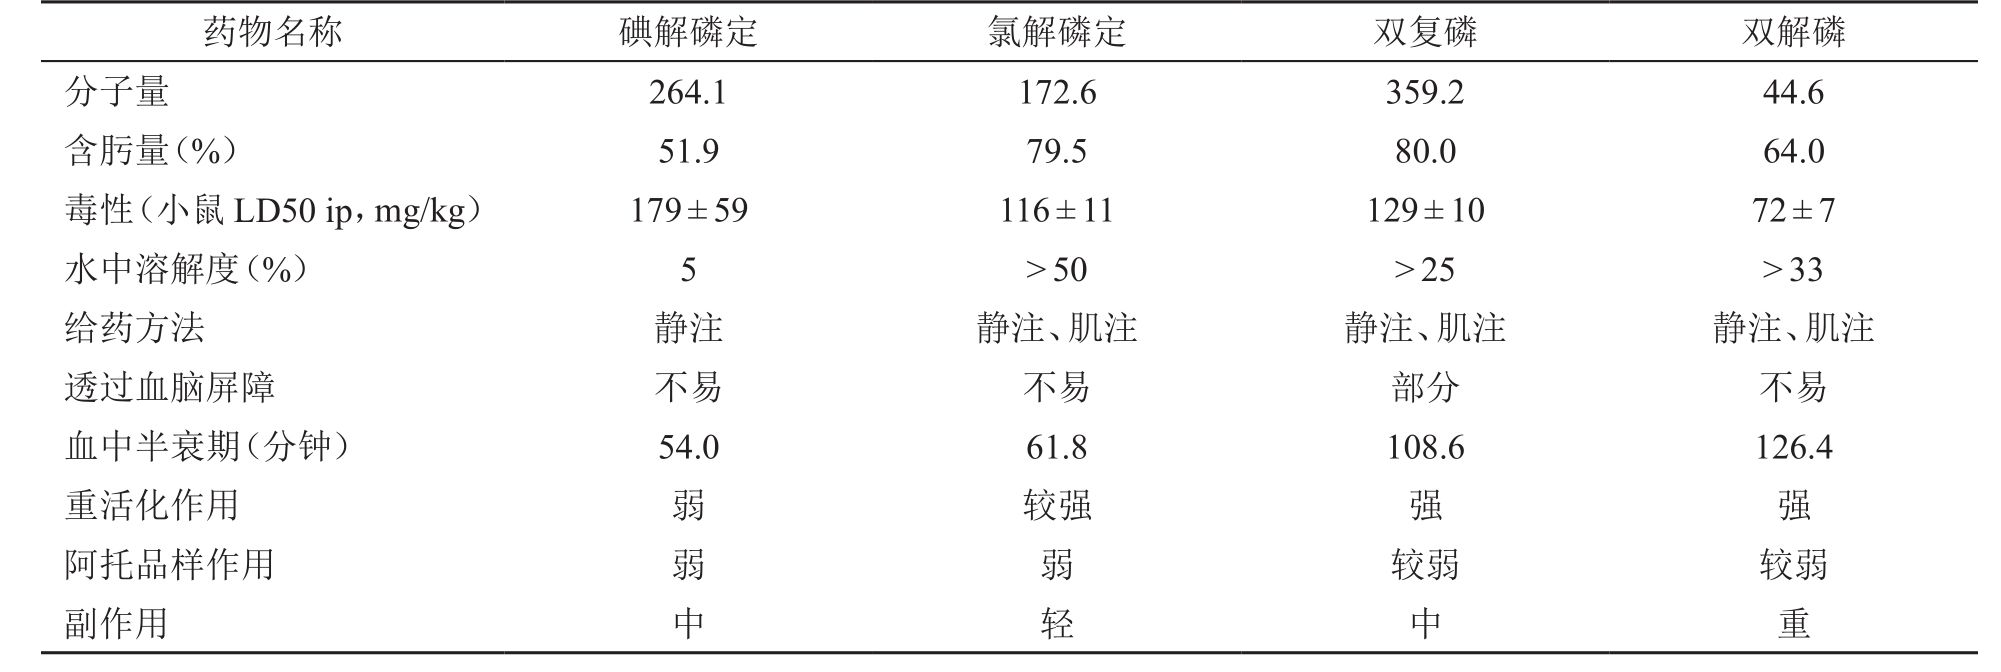
\includegraphics[width=6.66667in,height=2.22917in]{./images/Image00206.jpg}
\end{table}

中毒酶一般随时间的延长而“老化”,当中毒酶“老化”后,其活性不能再重活化。因此,重活化剂对中毒酶的重活化作用,在很大程度上取决于中毒后给药的时间,给药越早,作用越好。故一般认为中毒48小时后再给重活化剂,其疗效较差或无明显重活化作用。但近年研究表明,AOPP后仍存在有机磷农药持续重复吸收,代谢增毒,肝、肠循环等,不断有新的ChE被抑制,重活化剂的使用不应仅限于72小时内,应充分利用重活化剂的ChE重活化效应和非重活化效应。如口服大量乐果中毒、昏迷时间长、对ChE重活化剂疗效差及血ChE活性低者,解毒药维持剂量要大,时间可长达5~7天或以上。

\paragraph{首次应用重活化剂的剂量}

重活化剂只有首次足量用药,使体内尽快达到有效血药浓度时,对中毒酶活性才有较好重活化作用。氯解磷定和双复磷的有效血药浓度分别为大于4μg/ml和2μg/ml。如首次用量不足或者少量多次重复用药,均不易达到有效血药浓度。同时,肟类重活化剂为季铵化合物,脂溶性低,不易透过血脑屏障进入中枢神经系统;当首次给予较大剂量时,部分药物可渗透进入中枢神经而产生一定作用。因此,应用重活化剂时,应根据病情尽早首次足量给药(表\ref{tab55-5})。

\begin{table}[htbp]
\centering
\caption{常用肟类重活化剂(复能剂)首次应用剂量(g)\textsuperscript{*}}
\label{tab55-5}
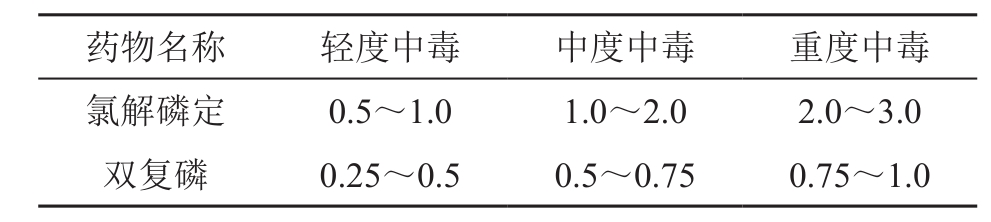
\includegraphics[width=3.29167in,height=0.72917in]{./images/Image00207.jpg}
\end{table}

*碘解磷定的剂量按氯解磷定剂量折算,1g氯解磷定相当于1.5g碘解磷定

\paragraph{有效血药浓度持续的时间}

重活化剂通过肾脏排出较快,其半衰期一般为1~1.5小时;因此,首次给药后应根据病情和药物的半衰期重复用药,维持有效血药浓度。硫胺(维生素B\textsubscript{1}
)能抑制解磷定和氯解磷定从肾小管排出,延长其半衰期而增加血药浓度。故当给予解磷定(iv)或氯解磷定(im)时,在前半小时内静脉滴注维生素B\textsubscript{1}
(硫胺)200mg,对于需要重复用药的严重中毒或口服中毒患者的治疗是一个有利的措施。

\paragraph{重活化剂的给药途径}

重活化剂口服给药吸收差,又不规则,一般采用静脉注射或肌肉注射。静脉注射虽然作用快,但药物排出也快,对维持较长时间的有效血药浓度不利。肌肉注射给药3~5分钟后一般可产生明显作用,且药物排出较慢,故一般情况又以肌注给药为宜。当患者有呼吸循环衰竭时,应采用静注给药,但不能采用静脉滴注给药。静脉滴注给药在短时内进入体内药物少,而且重活化剂半衰竭期短,排出快,不能达到有效血药浓度;因此,在急救治疗中,不宜采用静脉滴注给药。

\hypertarget{text00139.htmlux5cux23CHP5-3-1-3-2-2}{}
(二) 抗胆碱药

抗胆碱药主要作用于机体的胆碱能受体(ChR),它能和乙酰胆碱(ACh)争夺ChR,对抗ACh的作用,因而表现出胆碱能神经功能被阻滞的种种效应。故该类药又称为胆碱能受体阻滞药。

胆碱能受体(ChR)分为毒蕈碱型胆碱能受体(MChR)和烟碱型胆碱能受体(NChR),MChR从药理学上又分为M\textsubscript{1}
、M\textsubscript{2} 、M\textsubscript{3} 、M\textsubscript{4}
亚型,NChR分为N\textsubscript{1} (神经元型)、N\textsubscript{2}
(肌肉型)二种亚型(表\ref{tab55-6})。

\begin{table}[htbp]
\centering
\caption{胆碱能受体各亚型在体内的分布}
\label{tab55-6}
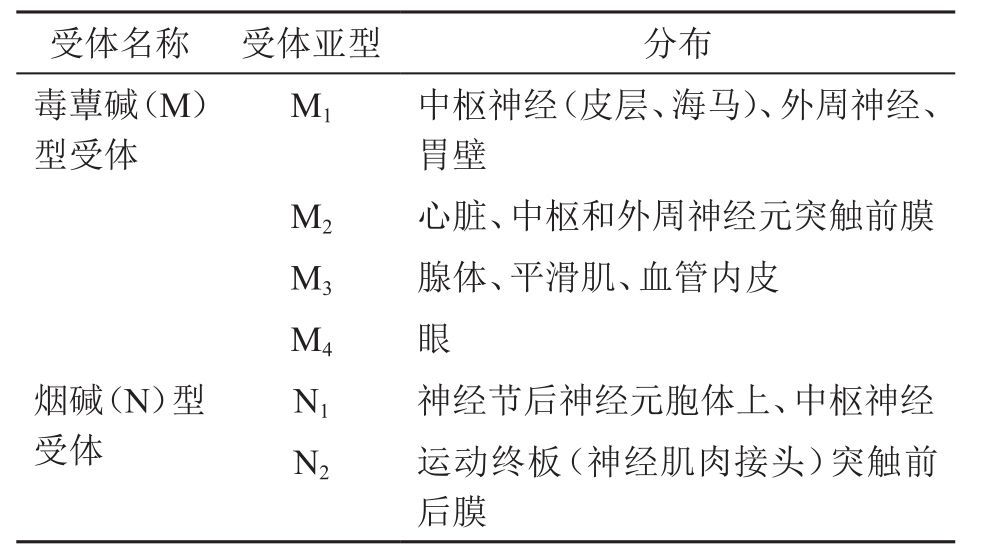
\includegraphics[width=3.27083in,height=1.83333in]{./images/Image00208.jpg}
\end{table}

有机磷毒物中毒后,ChE活性下降,导致过多的ACh作用于胆碱能受体(ChR)而出现毒蕈碱(M)样症状、烟碱(N)样症状和中枢神经系统症状。抗胆碱药能和ACh争夺ChR,阻断ACh作用,因而能对抗上述三类症状。但目前除盐酸戊乙奎醚外,还没有一个抗胆碱药能同时较好地对抗上述三类症状,而只能较好地对抗其中一类或二类症状;并且同一类的抗胆碱药对抗同一类症状的作用强弱和持续时间也各不相同。因此,只有取长补短同时伍用两个作用不同的抗胆碱药(如解磷注射液),才能较好、较全面地对抗有机磷农药中毒症状。然而,盐酸戊乙奎醚一个药便可出现上述疗效。根据药物作用的部位,临床上应用的抗胆碱药有:

\paragraph{M-胆碱受体阻断药(节后抗胆碱药)}

阿托品(atropine)为其典型代表。此外,还有山莨菪碱(654-2,anisodamine)和樟柳碱(AT\textsubscript{3}
,anisodine)等。

阿托品的外周作用主要是阻断节后胆碱能神经支配的效应器上的M-胆碱受体(M-ChR),因而能对抗ACh及各种拟胆碱药的毒蕈碱样症状。但由于阿托品对中枢的烟碱受体(N-ChR)无明显作用,故对有机磷毒物中毒引起的中枢神经症状,如惊厥、躁动不安和中枢呼吸抑制等,其对抗作用较差。同时,阿托品对骨骼肌及神经节的烟碱受体只有在给予极大剂量时才有作用,因而不能对抗有机磷农药中毒引起的肌颤(肉跳)和肌肉麻痹等。当中毒患者出现严重中枢呼吸抑制或中枢症状和外周呼吸麻痹时,阿托品的对抗作用是有限的,而必须伍用中枢抗胆碱药或其他药物来弥补其不足。

阿托品首次用量为:轻度中毒2.0~4.0mg,中度中毒5.0~10.0mg,重度中毒10.0~20.0mg,依病情每10~30分钟或1~2小时给药一次,直至患者M样症状消失或出现“阿托品化”。阿托品化指征为口干、皮肤干燥、心率稍快(90~100次/分)、瞳孔较前扩大和肺湿啰音消失,显示抗胆碱药用量足,此时,可暂停给药或给予维持量。如未出现上述指标,应尽快补充用药至出现上述指标为止。当中毒晚期ChE已“老化”或其活性低于50\%时,应给予适量抗胆碱药维持“阿托品化”,直至全血ChE活性恢复至50\%~60\%以上为止。如出现瞳孔明显扩大、神志模糊、烦躁不安、抽搐、昏迷和尿潴留等为阿托品中毒,立即停用阿托品。

瞳孔扩大和颜面潮红不是“阿托品化”的可靠指标。当中毒患者由呼吸道吸入中毒或眼局部染毒时,可出现瞳孔明显缩小,但全身给予超大剂量的阿托品或出现严重阿托品中毒,其瞳孔也不出现明显扩大。同时,大约有30\%的中毒患者由于多种原因,应用阿托品后不出现瞳孔扩大。中毒患者经给予一定剂量抗胆碱药如阿托品后,一般可出现颜面潮红;但如再继续不断地给予大剂量阿托品时,患者的颜面潮红可转苍白和出现四肢发冷,而常常误认为阿托品用量不足。

\paragraph{中枢性抗胆碱药}

常用的有东莨菪碱(scopolamine)和贝那替秦(benactyzine)。此外,还有苯扎托品(benztropine)和丙环定(procyclidine)等。

这类药物和阿托品等不同之处,是对中枢神经毒蕈碱受体(M-ChR)和烟碱样受体(N-ChR)均有明显作用,故有较强的中枢作用。因此,它们不仅和阿托品一样,能对抗有机磷农药中毒引起的毒蕈碱样症状,而且还能较好地减轻或消除有机磷农药中毒出现的躁动不安、惊厥和中枢呼吸抑制。这类药物常用剂量也不能对抗外周烟碱样中毒症状;当用于救治严重中毒患者时,也必须同时伍用重活化剂或其他药物。它们用于救治有机磷毒物中毒的首次剂量见表\ref{tab55-7}。

\begin{table}[htbp]
\centering
\caption{抗胆碱药用于有机磷农药中毒患者的首次用量(mg)}
\label{tab55-7}
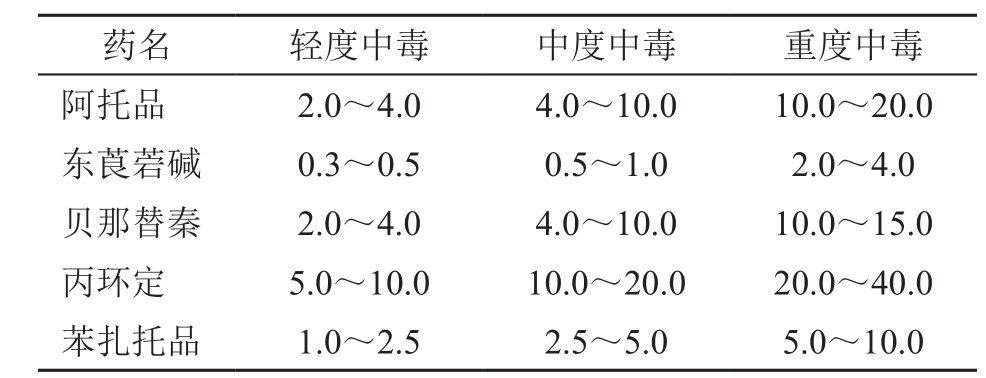
\includegraphics[width=3.27083in,height=1.25in]{./images/Image00209.jpg}
\end{table}

*两药伍用时,各用半量;重复用药时,采用轻度中毒剂量

\paragraph{新型抗胆碱药盐酸戊乙奎醚}

盐酸戊乙奎醚主要选择性作用于M胆碱能受体亚型M\textsubscript{1}
、M\textsubscript{3} ,而对M\textsubscript{2} 、M\textsubscript{4}
无明显作用或作用较弱;其主要作用部位是中枢神经、腺体和平滑肌等,而对心脏或神经元突触前膜M\textsubscript{2}
和瞳孔无明显作用或作用较弱。中枢和外周神经元突触前膜的M\textsubscript{2}
受体称为自身受体,通过负反馈调控神经末梢递质(ACh)释放,即当释放的ACh过多时,可抑制ACh的释放。可见突触前膜M\textsubscript{2}
受体在保持正常生理功能中发挥了重要的效应,当其M\textsubscript{2}
受体的效应被阻断或破坏时,必然药物效应减弱和导致一系列有害或不良反应。阿托品正由于对M\textsubscript{1}
、M\textsubscript{2} 、M\textsubscript{3} 、M\textsubscript{4}
受体均有作用(无选择性),故常常疗效和许多不良反应同时出现;当用药剂量过大或应用时间过长时,则更易出现突触前膜ACh释放增多和突触后膜M受体上调(受体数目增多),而导致效应或疗效减弱和出现一系列有害反应,如肺水肿、脑水肿等胆碱能危象和阿托品依赖等。而盐酸戊乙奎醚正由于对M\textsubscript{2}
、M\textsubscript{4}
受体无明显作用或作用较弱,故在临床上应用时,不易出现心动过速、瞳孔扩大和阻断突触前膜M\textsubscript{2}
受体调控神经末梢释放ACh的功能。这为临床上所见盐酸戊乙奎醚的不良反应比阿托品轻或少,提供了有力的药理依据。

盐酸戊乙奎醚抗胆碱作用的特点是:对外周M受体和中枢M、N受体均有作用,但选择性作用于M\textsubscript{1}
、M\textsubscript{3} 受体亚型,对M\textsubscript{2}
受体作用极弱,对心率无明显影响;较阿托品作用强,有效剂量小,作用时间(半衰期6~8小时)长,不良反应少。首次用量为:轻度中毒1.0~2.0mg,中度中毒2.0~4.0mg,重度中毒4.0~6.0mg。首次用药需与氯解磷定合用。

盐酸戊乙奎醚伍用氯解磷定救治有机磷中毒的实施方法:①患者确诊后,立即按轻、中、重度中毒肌注给药,除轻度中毒外,盐酸戊乙奎醚首次用药均须与氯解磷定伍用,其用法与用量见表\ref{tab55-8}。②首次给药30分钟后,如中毒症状尚未明显消失和全血胆碱酯酶(ChE)活性低于50\%时,再给予(肌注)首次用药的半量(参见表\ref{tab55-8});如中毒症状明显消失和全血ChE活性恢复至50\%以上时,可暂停药观察。③首次给药后1~2小时,如中毒症状仍未明显消失或又重新出现和全血ChE活性低于50\%时,再给首次用药的半量。④中毒患者病情基本好转后,如仅有部分毒蕈碱(M)样症状(恶心、呕吐、出汗、流涎等),可肌注盐酸戊乙奎醚1~2mg;如仅有烟碱(N)样症状(肌颤等)或全血ChE活性低于50\%,可肌注氯解磷定0.5~1.5g。⑤中毒48小时后如ChE已老化或中毒症状基本消失但全血ChE活性仍低于50\%以下时,应酌情肌注盐酸戊乙奎醚1~2mg(每6~12小时1次),维持“阿托品化”或“长托宁化”至ChE活性恢复至50\%~60\%以上。⑥中毒症状基本消失和全血ChE活性恢复至60\%以上(含60\%)可停药观察,停药12~24小时如ChE活性仍保持在60\%以上可考虑出院。

\begin{table}[htbp]
\centering
\caption{成人药物的用法与用量\textsuperscript{*}}
\label{tab55-8}
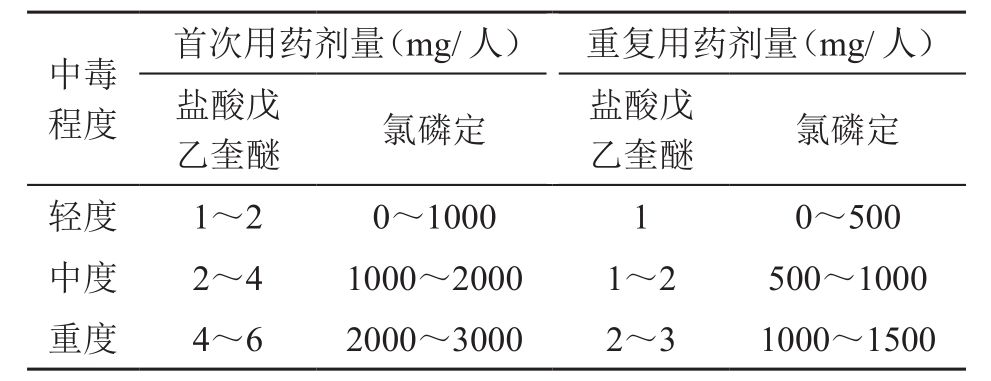
\includegraphics[width=3.29167in,height=1.26042in]{./images/Image00210.jpg}
\end{table}

*小儿按体表面积折算剂量法折算用量

\hypertarget{text00139.htmlux5cux23CHP5-3-1-3-2-3}{}
(三) 复方制剂

\paragraph{解磷注射液}

每支含阿托品3mg、苯那辛3mg和氯解磷定400mg。首次剂量:轻度中毒1/2~1支肌注;中度中毒1~2支;重度中毒2~3支。但尚需分别另加氯解磷定,轻度中毒0~0.5g,中度中毒0.5~1.0g,重度中毒1.0~1.5g。

\paragraph{苯克磷注射液}

由甲磺酸苯扎托品(苯甲托品)、丙环定(开马君)和双复磷组成。针剂每支2ml,仅供肌注。首剂:轻度中毒1~2ml肌注;中度中毒2~4ml;重度中毒4~6ml。在30~60分钟,视临床表现和全血ChE活力酌情再用,一般只用1~2次,最多3次。

急性有机磷农药中毒,一般当全血ChE活性被抑制50\%以上时,可出现明显中毒症状。急性中毒后血液ChE活性的改变比组织的ChE活性改变较快,故常常通过简便易行的全血ChE活性测定来观察病情改变和预后。当中毒患者经急救治疗后,主要的中毒症状基本消失,全血ChE活性恢复至50\%~60\%以上时,可停药观察;如停药12~24小时以上,其ChE活性仍保持在60\%以上时,可出院。但重度中毒患者通常至少观察3~7天再出院。

\subsubsection{对症支持治疗}

包括:①保持呼吸道通畅:吸除气道分泌物,给氧;对昏迷患者,须气管插管,呼吸衰竭时进行人工通气。②维持循环功能:包括抗休克治疗、纠正心律失常等。③镇静抗惊:早期使用地西泮(diazepam),能间接抑制中枢乙酰胆碱的释放,并通过阻滞钙通道抑制神经末梢发放异常冲动,保护神经肌肉接头。AOPP使用地西泮可起到镇静、抗焦虑、肌肉松弛、抗惊厥和保护心肌的作用。可用于经解毒治疗后仍有烦躁不安、抽搐的患者,用法为10~20mg肌肉注射或静脉注射,必要时可重复。注意用量过大或静脉注射速度过快可产生呼吸抑制。④防治脑水肿、抗感染、维持水电解质酸碱平衡等,详见有关章节。

\subsubsection{血液净化疗法}

对重度中毒,尤其是就医较迟、洗胃不彻底、吸收毒物较多者,可行血液灌流或血浆置换治疗。

\hypertarget{text00139.htmlux5cux23CHP5-3-1-4}{}
参 考 文 献

1. 陆再英,钟南山.内科学.第7版.北京:人民卫生出版社,2008

2. 张文武.急诊内科手册.北京:人民卫生出版社,2009

3. 曾繁忠
.盐酸戊乙奎醚(长托宁)取代阿托品救治有机磷农药中毒技术.北京:军事医学科学出版社,2004

\protect\hypertarget{text00140.html}{}{}

\section{拟除虫菊酯类农药中毒}

拟除虫菊酯类农药(pyrethroids
pesticides)为人工合成的类似天然除虫菊素的化学结构的一类农药。其分子由菊酸和醇两部分组成。多难溶于水,易溶于有机溶剂。在酸性介质中稳定,遇碱性易分解失效。品种繁多,基本上可分为两类:化学结构中不含α-氰基的拟除虫菊酯为Ⅰ型,如苄呋菊酯(resmethrin),氯菊酯(permethrin)、烯丙菊酯(allethrin)等属低毒物质,主要用作卫生杀虫剂,罕见急性中毒病例;含α-氰基的拟除虫菊酯为Ⅱ型,如溴氰菊酯(deltamethrin,敌杀死)、氰戊菊酯(fenvalerate,速灭菊酯,速灭杀丁,来福灵)、氯氰菊酯(cypermethrin,安绿定,灭百可)等,毒性中等,一般配成乳油用作农业杀虫剂。

\subsection{病因与中毒机制}

本类农药可经呼吸道、皮肤及胃肠道吸收。生产性中毒最多为农药喷洒者和农药厂工人,主要由皮肤污染进入,少数由呼吸道吸入;生活性中毒大都经口有意摄入,极少数为误将本类杀虫剂制作的安瓿(以氰戊菊酯为多)当成医药而误注射中毒。在体内迅速分布到各器官组织,在肝内经酯酶和混合功能氧化酶作用而降解。其代谢产物主要肾排出。本品属于神经毒物,主要作用于中枢神经系统的锥体外系、小脑、脊髓和周围神经。有增强中枢神经和周围神经作用,其作用机制可能与它减慢神经细胞膜钠离子通道“M”闸门的关闭,并阻滞氯离子通道的开放有关;也有人认为本类农药可作用于中枢神经的γ-氨基丁酸(GABA)受体,使GABA丧失对大脑的抑制功能,从而使脑的兴奋性相对增高。此外,对局部皮肤有明显的刺激作用,可导致接触性皮炎及过敏反应。

本品水解可被有机磷农药在体内或体外所抑制,因此先后或同用这两种杀虫剂能协同增强杀虫剂的效果及其急性毒性。

\subsection{诊断}

\paragraph{病史}

有短期密切接触较大剂量或口服拟除虫菊酯史。

\paragraph{临床表现特点}

\hypertarget{text00140.htmlux5cux23CHP5-3-2-2-2-1}{}
(1) 生产性中毒:

潜伏期短者1小时,长者可达24小时,平均6小时。田间施药中毒多在4~6小时起病,主要表现为皮肤黏膜刺激症状,体表污染区感觉异常(颜面、四肢裸露部位及阴囊等处),包括麻木、烧灼感、瘙痒、针刺和蚁行感等,系周围神经兴奋性增高的表现,停止接触数小时或十余小时后即可消失。常有面红、流泪和结膜充血,部分病例局部有红色丘疹样皮损。眼内污染立即引起眼痛、羞光、流泪、眼睑红肿和球结膜充血。呼吸道吸收可刺激鼻黏膜引发喷嚏、流涕,并有咳嗽和咽充血。全身中毒症状相对较轻(最迟48小时后出现),多为头晕、头痛、乏力、肌束震颤及恶心、呕吐等一般神经和消化道症状,但严重者也有流涎、肌肉抽动甚至抽搐,伴意识障碍和昏迷。

\hypertarget{text00140.htmlux5cux23CHP5-3-2-2-2-2}{}
(2) 口服中毒:

多在10分钟~1小时出现中毒症状,先为上腹部灼痛、恶心、呕吐等消化道症状,可发生糜烂性胃炎。继而食欲不振、精神萎靡或肌束震颤,部分患者口腔分泌物增多,尚可有胸闷、肢端发麻、心慌、视物模糊、多汗等。重度中毒者出现阵发性抽搐,类似癫痫大发作,抽搐时上肢屈曲痉挛、下肢挺直、角弓反张,伴意识丧失,持续约1/2~2分钟,抽搐频繁者每日发作可多达10~30次,各种镇静、止痉剂常不能明显奏效,可持续10~20天。也有无抽搐即意识障碍直至昏迷者。对心血管的作用一般是先抑制后兴奋,开始心律减慢,血压偏低,其后可转为心率增快和血压升高,部分病例尚伴其他心律失常。个别病例有中毒性肺水肿。

\paragraph{实验室检查}

\hypertarget{text00140.htmlux5cux23CHP5-3-2-2-3-1}{}
(l)毒物检测:

拟除虫菊酯原形物质排泄迅速,停止接触12小时后在接触人员的尿中就难以测出。但其代谢产物可检测出的时间较长(2~5天)。有条件时可作毒物或其代谢产物检测。

\hypertarget{text00140.htmlux5cux23CHP5-3-2-2-3-2}{}
(2) 全血ChE活性:

无明显变化,有助于与急性有机磷农药中毒(AOPP)鉴别。

\hypertarget{text00140.htmlux5cux23CHP5-3-2-2-3-3}{}
(3) 心电图检查:

少数中毒患者ST段下降及T波低平,窦性心动过缓或过速,室性期前收缩或房室传导阻滞等。

\paragraph{急性中毒分级}

①轻度中毒:常有头晕、头痛、恶心、呕吐、食欲缺乏、乏力、流涎、心慌、视力模糊、精神萎靡等,但体检无阳性发现。口服中毒者消化道症状更明显,可有上腹部灼痛及腹泻等。②中度中毒:除上述症状外,尚有嗜睡、胸闷、四肢肌肉震颤、心律失常、肺部啰音等。③重度中毒:有呼吸增快、呼吸困难、心悸、脉搏增快、血压下降、阵发性抽搐或惊厥、角弓反张、发绀、肺水肿和昏迷等。病情迁延多日,危重者可致死亡。

\paragraph{鉴别诊断}

需要鉴别的疾病有中暑、上呼吸道感染、食物中毒、脑卒中、原发性癫痫或其他急性农药中毒等。因本品的气味与有机磷相似,尤其应与AOPP相鉴别,除依据接触史外,本品中毒全血ChE活性大多正常,且多数不能耐受5mg以上阿托品治疗,一般预后较好,毒物检测有助于鉴别。

\subsection{治疗}

\paragraph{清除毒物}

生产性中毒者,应立即脱离现场,将患者移至空气新鲜处,脱去染毒的衣物,用肥皂水或2\%~4\%碳酸氢钠溶液彻底洗胃,然后用50\%硫酸钠40~60ml导泻,并经胃管灌入活性炭30~50g吸附残余毒物。对有频繁抽搐、意识障碍或昏迷、中毒性肺水肿等表现的严重中毒病例,应尽早作血液灌流或血液透析治疗。

\paragraph{控制抽搐}

常用地西泮或巴比妥类肌注或静注。抽搐未发生前可预防性使用,控制后应维持用药防治再抽搐。动物实验研究发现异戊巴比妥能开放本品所关闭的氯离子通道,而苯巴比妥对氯离子通道则无此作用,故异戊巴比妥控制本品中毒所致抽搐的疗效明显优于苯巴比妥。抽搐发作时,可用地西泮10~20mg或异戊巴比妥钠(阿米妥)0.1~0.3g静注。亦可用苯妥英钠0.1~0.2g肌注或静注,本品尚可诱导肝微粒体酶系,有利于加速拟除虫菊酯类农药的代谢解毒。

\paragraph{解毒治疗}

无特效解毒剂,下述药物可试用:

\hypertarget{text00140.htmlux5cux23CHP5-3-2-3-3-1}{}
(1) 中枢性肌松剂:

动物实验发现唛酚生(mephenesin)对溴氰菊酯有较好的抗毒作用,美索巴莫(舒筋灵)(methocarbamol)也有很好的抗毒和保护作用,贝克洛芬(beclofen)对氰戊菊酯动物中毒有显著疗效。三种均为中枢性肌松剂,选择性抑制脊髓神经的兴奋,但缺乏人体中毒的疗效验证,尚待进一步临床使用与研究。舒筋灵0.5肌注,或贝克洛芬10mg肌注,每日2次,连用3天。

\hypertarget{text00140.htmlux5cux23CHP5-3-2-3-3-2}{}
(2) 中药葛根素和丹参:

对实验中毒动物有保护和治疗作用,已试用于临床,对控制症状和缩短疗程有一定的疗效。葛根素静脉滴注5mg/kg,2~4小时重复一次,24小时用量不宜大于20mg/kg,症状改善后改为每日1~2次,直至症状消失。亦可用复方丹参注射液治疗。

\hypertarget{text00140.htmlux5cux23CHP5-3-2-3-3-3}{}
(3) 阿托品:

只能用于控制流涎和出汗等症状,0.5~1.0mg肌肉注射,发生肺水肿时可增大至每次1~2mg,但总量不宜过大,达到控制症状即可。切不可企图用阿托品来做解毒治疗,否则将加重抽搐,甚至促进死亡。

\paragraph{对症支持治疗}

静脉输液加速毒物排泄,酌情选用能量合剂、肾上腺皮质激素、维生素B\textsubscript{6}
、维生素C等药物,维持水电解质和酸碱平衡,选用抗生素防治感染等。

\protect\hypertarget{text00141.html}{}{}

\section{氨基甲酸酯类农药中毒}

氨基甲酸酯类农药(carbamate
insecticides)是继有机氯、有机磷农药后的一种较新型的有机杀虫剂,是有机氮农药的一种,用作农业上的有杀虫剂、除草剂、杀菌剂等。杀虫剂农药可分为五大类:①萘基氨基甲酸酯类,如西维因(carbaryl);②苯基氨基甲酸酯类,如叶蝉散(isoprocarb);③氨基甲酸肟酯类,如涕灭威(aldicarb);④杂环甲基氨基甲酸酯类,如呋喃丹(carbofuran);⑤杂环二甲基氨基甲酸酯类,如异索威(isolan)。除草剂农药有禾大壮、禾草丹、除草丹、灭草灵、燕麦灵等。具有高效、作用快、残毒低、对昆虫选择性较强、易分解、体内无蓄积等特点。本类农药无特殊气味,在酸性条件下稳定,遇碱则易分解失效。除少数品种如呋喃丹、涕灭威等毒性较高外,大多数属中、低毒性。呋喃丹中毒为其代表。

\subsection{病因与中毒机制}

氨基甲酸酯类农药可经呼吸道、皮肤和消化道吸收,主要分布在肝、肾、脂肪和肌肉组织中。在肝进行代谢,一部分经水解、氧化或与葡萄糖醛酸结合而解毒,一部分以原形或其代谢产物迅速由肾排泄,24小时可排出摄入量的90\%以上。中毒机制是其可与ChE阴离子和酯解部位结合,形成可逆性的复合物,即氨基甲酰化,使其失去对ACh的水解能力,致Ach蓄积产生相应的临床表现。但氨基甲酰化ChE易水解,使ChE活性于4小时左右自动恢复。因此,尽管中毒开始病情较重,一旦脱离接触,胆碱酯酶即很快复能,症状也很快消失,24小时内几乎完全恢复正常。

一次接触大剂量氨基甲酸酯类农药中毒后,血ChE活力在15分钟下降至最低水平,30~40分钟后可恢复到50\%~60\%,60~120分钟后血ChE活力基本恢复正常。随着血ChE活力的恢复,临床症状很快好转和消失。反复接触氨基甲酸酯类农药,血ChE活力可抑制到50\%,而临床可无中毒症状。

应用肟类复能剂不仅不能帮助氨基甲酰化ChE的复能,反而会妨碍受抑制酶的自动复能,因此,氨基甲酸酯类农药中毒禁用肟类复能剂。

\subsection{诊断}

\paragraph{毒物接触史}

有氨基甲酸酯类农药接触史。

\paragraph{临床表现特点}

本类农药中毒临床表现与有机磷农药中毒类似,但其具有潜伏期短、恢复快、病情相对较轻,只要彻底清除毒物,病情通常无反复等特点。经皮吸收中毒潜伏期大约为0.5~6小时,经口中毒多在10~30分钟内发病。主要表现有头晕、头痛、乏力、恶心、呕吐、流涎、多汗、瞳孔缩小,严重者可出现呼吸困难、肌颤、腹痛、腹泻、意识障碍、抽搐、惊厥、发绀、昏迷、大小便失禁等,可因呼吸麻痹致死,死亡多发生于中毒发作后的12小时内。经皮中毒局部皮肤可有潮红,甚至出现皮疹,乃药剂的直接刺激作用所致。中毒程度分级可参照有机磷中毒的分级标准划分。

\paragraph{辅助检查}

中毒后全血胆碱酯酶活性降低;呕吐物或清洗液中可测到相应的毒物。

\subsection{治疗}

\paragraph{清除毒物}

生产性中毒者应迅速脱离中毒环境,除去染毒衣物,用肥皂水或2\%碳酸氢钠溶液清洗染毒部位。经口中毒者,立即用清水或2\%碳酸氢钠液洗胃,然后注入50\%硫酸钠50ml导泻。

\begin{table}[htbp]
\centering
\caption{氨基甲酸酯类农药(呋喃丹)中毒阿托品剂量与用法参考表}
\label{tab55-9}
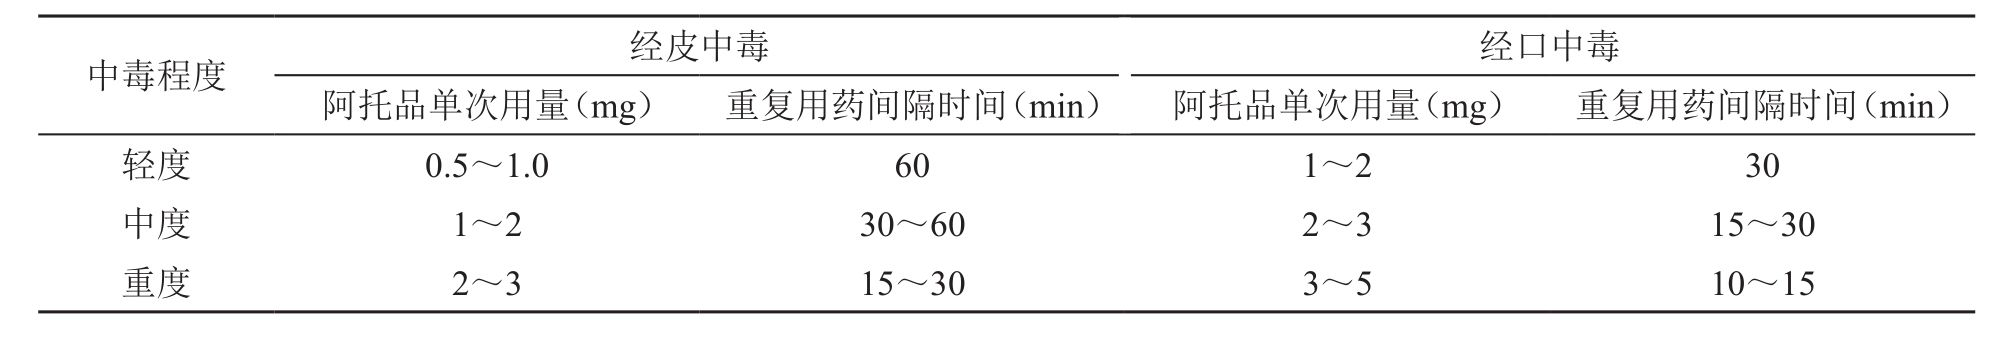
\includegraphics[width=6.66667in,height=1.13542in]{./images/Image00211.jpg}
\end{table}

\paragraph{解毒治疗}

应及早应用阿托品类药物,禁用肟类复能剂;但如系本品与有机磷农药混合中毒,则往往先有较短期的氨基甲酸酯农药中毒阶段,继之出现较长而严重的有机磷农药中毒过程,可先用阿托品,在中毒一段时间后可酌情适量使用复能剂。中毒初始6~8小时,阿托品的用法与用量可参考表\ref{tab55-9}。一般轻或中度中毒可肌注给药;严重中毒则应静注。轻、中度中毒不需要阿托品化;经口严重中毒必要时可考虑阿托品化至病情明显好转后再减量维持,切忌盲目大量投药,谨防阿托品中毒。6~8小时后,轻、中度中毒可用0.5~1.0mg阿托品,每4~6小时重复维持;严重中毒每2~4小时用阿托品1~2mg,全部维持用药时间24小时左右即可。

东莨菪碱对氨基甲酸酯类农药中毒的治疗效果可能优于阿托品。因为前者对腺体、睫状肌、虹膜括约肌上的M受体阻滞作用强于阿托品,且小剂量时可兴奋呼吸中枢,防止呼吸衰竭;而大剂量时具有明显的催眠作用,故不易导致惊厥。用法:东莨菪碱0.01~0.05mg/kg,静注或肌注,每30分钟1次,至症状缓解后减量维持治疗24小时左右。

\paragraph{对症治疗}

中毒严重者可选用皮质激素以抑制应激反应,防治肺水肿、脑水肿、支气管痉挛和休克。抽搐者宜选用地西泮治疗,而不宜用巴比妥类药物,因后者是肝微粒体多功能氧化酶的诱导剂,会促进毒物氧化,对毒物快速解毒不利。保持呼吸道通畅,必要时行气管切开。维持水电解质平衡,选用适当的抗生素。接触性皮炎按皮肤科诊治原则处理。

\protect\hypertarget{text00142.html}{}{}

\section{甲脒类农药中毒}

甲脒类(formamidines)农药是一种广谱的杀虫剂和杀螨剂,主要用于防治水稻螟虫和棉花红铃虫、果树螨类,属低残留、中等毒类农药。包括杀虫脒(chlordimeform)、单甲脒和双甲脒(双虫脒、灭螨胺)等。代表品种是杀虫脒,它的中间体和代谢产物对人有致癌作用,故于1988~1989年国内外都作出停止生产杀虫脒的决定,但仍有非法生产和使用而发生中毒者。单甲脒和双甲脒仍然是广泛生产和使用的甲脒类农药,前者是在杀虫脒的苯环上对位氯被甲基取代所致,后者则为两个单甲脒分子连接而成。因此,其毒性、毒理、中毒的临床表现和救治方法均与杀虫脒中毒相同。

\subsection{病因与中毒机制}

杀虫脒又名氯苯脒或杀螨脒,可经皮肤、呼吸道进入人体,也有误服中毒者。入体后能迅速吸收,主要分布于肝、肾、肺、脑等器官,代谢迅速。经氧化产生的代谢产物N-甲酰基氯邻甲苯胺和4-氯邻甲苯胺为有毒物质。毒物进入机体后,以其原型及代谢产物从肾脏及消化道排出,在体内无明显蓄积作用。

杀虫脒及其代谢产物:①能使体内的正常血红蛋白变成高铁血红蛋白,使之失去携氧能力,导致组织缺氧;②化学结构类似利多卡因,故有麻醉作用,使中毒者有明显的嗜睡现象,且可抑制心肌收缩及血管运动中枢,导致血压下降等休克症状;③经肾脏排出,可损伤泌尿道黏膜,造成出血性膀胱损害。④能抑制线粒体三磷腺苷酶的氧化磷酸化作用,干扰能量代谢,影响心、肝、肾功能,出现心肌收缩乏力、心肌炎、心力衰竭、肝功能损害、蛋白尿及血尿。此外,杀虫脒可抑制单胺氧化酶的活性,导致脑内5-羟色胺浓度增高;加之脑组织缺氧,脑血管呈麻痹样扩张,血管通透性增加,导致脑水肿,颅压增高,患者呈昏迷状态。

\subsection{诊断}

1.有杀虫脒农药接触史。

2.临床表现特点
急性杀虫脒中毒潜伏期短,经皮肤吸收平均6小时左右,最快2小时左右即发病;经口误服0.5~1小时发病。中毒后出现全身性多脏器受累表现,其中以嗜睡、发绀、出血性膀胱炎三大综合征为主要表现。心力衰竭、脑水肿及呼吸衰竭是常见的致死原因。

(l)神经系统:开始有头晕、头痛、乏力、肌肉酸痛、肢体麻木及眩晕等,稍后则出现视物模糊、步态不稳、肌肉震颤、癔症样抽搐、嗜睡及昏迷等,其中以嗜睡较突出。少数昏迷者治疗清醒后可出现幻觉、偏执等精神症状。重症可出现呼吸暂停或叹气样呼吸。

(2)
发绀:主要因高铁血红蛋白血症所致。以口唇、鼻尖、四肢末端发绀明显,无气促是其中毒特点之一。发绀程度与中毒剂量成正比。

(3)
泌尿系统:多于中毒后12~48小时出现尿频、尿急、尿痛等膀胱刺激症状,尿中几乎100\%有血尿及白细胞,但多无管型。

(4)
循环系统:重者可出现心衰及肺水肿、心源性休克、心音低钝、心率减慢,ST-T改变、QT延长,大多为可逆性损害,多于5~15天内恢复。个别患者发生猝死。

(5)
消化系统:有恶心、呕吐及明显厌食,少数病例有上消化道出血,尤其与有机磷混合中毒者较为多见,其中以明显厌食较为突出。部分病例恢复期有一过性轻度肝功能异常。

(6)
局部症状:严重污染局部皮肤有麻木、烧灼感、疼痛感、局部充血、瘙痒及痱子样丘疹等,乃由药液直接刺激所致。

3.辅助检查
①变性血红蛋白测定阳性;②红细胞中可发现有海因(Heinz)小体;③血胆碱酯酶活性测定正常;④尿中有杀虫脒及其代谢物4-氯邻甲苯胺。

4.急性中毒分级 ①轻度中毒:表现为嗜睡,血中高铁血红蛋白浓度<
30\%;②中度中毒:发绀与实质性脏器功能损害,血中高铁血红蛋白浓度为30\%~60\%;③重度中毒:昏迷,有呼吸、循环、肾功能衰竭,血中高铁血红蛋白浓度>
60\%。

5.诊断注意事项
本品中毒应注意与农药氯酸钠、敌稗、除草醚等中毒所致的化学性青紫和AOPP鉴别。

\subsection{治疗}

\paragraph{清洗毒物}

杀虫脒在碱性环境中易被破坏。对皮肤染毒者,立即脱去污染衣物,用肥皂水清洗皮肤。对经口中毒者,可采用1\%~2\%碳酸氢钠液反复洗胃,洗胃后灌入活性炭50~100g。

\paragraph{解毒治疗}

无特殊的拮抗药。高铁血红蛋白血症使用小剂量亚甲蓝、大剂量维生素C、高渗葡萄糖和辅酶A治疗。亚甲蓝每次按1~2mg/kg加入50\%葡萄糖20~40ml中,缓慢(>
10~15分钟)静注,必要时l~2小时重复半量,每次量不宜超过200mg,24小时总量勿超过600mg。另外,维生素C、硫代硫酸钠对高铁血红蛋白有还原作用,可在输液中持续静滴,一般不如亚甲蓝可靠。维生素B\textsubscript{12}
、辅酶A及高渗葡萄糖,可增强亚甲蓝的还原作用。

\paragraph{对症治疗}

出血性膀胱炎可用酚磺乙胺(止血敏)、肾上腺色腙(安络血)等止血剂,必要时用少量肾上腺皮质激素;在输液和利尿的同时用碳酸氢钠碱化尿液,选用对肾脏无损害的抗生素预防尿路感染。意识障碍者,给予脑代谢活化剂、能量合剂及复苏药物;重症者可给氧,气管插管,呼吸兴奋剂。及时处理电解质紊乱、消化道出血、溶血性贫血、脑水肿等并发症。应注意,除非与有机磷农药混用中毒,不要用阿托品来作解毒治疗。

\protect\hypertarget{text00143.html}{}{}

\section{沙蚕毒素类农药中毒}

沙蚕毒素类(nereistoxines)农药是仿照天然沙蚕毒素(nereistoxin,NTX,是存在于海生环节动物沙蚕体内的一种有杀虫性能的神经毒物)的化学结构,人工合成的一类仿生性杀虫剂农药(NTX
insecticides,NTXI)。目前已投入使用的有巴丹(杀螟丹)、杀虫双、杀虫环(易卫杀)和杀虫蟥等。本类农药纯品多为白色结晶固体,易吸潮,在水中溶解度较大,故可制成水剂,如市售杀虫双即为25\%水剂,呈暗棕色。在酸性介质中稳定,而在碱性环境尤其是强碱条件下,易分解失效。大多为中等毒性,对皮肤黏膜一般无明显刺激作用,急性中毒多为经口所致。

\subsection{病因与中毒机制}

本类农药在体内吸收、代谢转化和排出均比较快。体内氧化水解为有毒的沙蚕毒素或二氢沙蚕毒素,易透过血脑屏障对中枢神经系统起毒害作用。其主要中毒机制是在神经突触处竞争性地占据胆碱能神经递质的受体,阻断胆碱能神经的突触传导;在剂量较小时以周围性神经-肌接头阻滞作用为主,大剂量则可直接作用于中枢神经系统。本类农药在占据受体时,是以它的硫醇基团({}
)与受体的巯基形成二硫键({}
)从而占据受体,体内很多具有重要功能的巯基酶,也可通过形成二硫键而受到损害,但此类影响是可逆的。此外,尚有轻微的抗胆碱酯酶活性作用,但这不是主要的中毒机制。

\subsection{诊断}

\paragraph{病史}

有本类农药的接触史或口服史,须注意与急性有机磷农药、氨基甲酸酯类农药中毒等相鉴别。

\paragraph{临床表现特点}

人类喷洒时吸入和大面积皮肤污染吸收虽可引起急性中毒,但很少见,这与本类农药经皮毒性甚小有关。绝大多数中毒由经口误服所致,其中毒潜伏期短,约0.5~l小时发病。主要表现有头晕、眼花、头痛、恶心、呕吐、中上腹不适感、心悸、烦躁、乏力、麻木、视物模糊、面色苍白、流涎、出汗等,严重者可有全身肌肉抽动或肌肉麻痹(包括呼吸肌),甚至发生惊厥和昏迷,也可发生肺水肿,瞳孔可见缩小等。大量误服尚可引起心、肝、肾等脏器损害。全血ChE活性有所下降,但均在正常人的50\%以上。死亡原因主要为呼吸衰竭和(或)心肌损害所致的严重心律失常,但死亡率甚低。所有中毒症状包括昏迷在内均延续不太久,可逐渐减轻,如能安全渡过急性期(24小时内)多可顺利恢复;但如大量经口误服,延误治疗,也可由呼吸麻痹等致死,常发生于中毒后的12小时内,甚至更短。

\subsection{治疗}

1.清除毒物
口服中毒者应首选碱性液体洗胃,洗胃后予以导泻。杀虫双口服中毒宜用0.02\%高锰酸钾溶液洗胃,高锰酸钾能迅速分解杀虫双为无毒或低毒的硝酸盐和硫酸盐等。

2.解毒治疗
可使用阿托品,除拮抗M受体兴奋的毒作用外,对本类农药占据神经-肌肉接头受体可能有竞争性阻断作用。一般病例可用0.5~1.0mg肌注或静注,1~4小时1次;重症者可用2~3mg,0.5~1小时1次,无需阿托品化,维持用药时间一般不超过3天。对有烦躁不安者,可改用东莨菪碱。此外,巯基类络合剂也可用于解毒治疗,能恢复被NTX阻遏的神经肌肉接头的冲动传递,拮抗呼吸抑制作用,但对中枢神经系统症状无治疗作用。可选用L-半胱氨酸,每次0.1g肌注,每日1~2次,用2~3天即可;也可选用二巯丙磺钠(0.25g肌注或静注,6~8小时1次,每日2~3次)或二巯丁二酸钠等药物。禁用肟类复能剂,否则将加重ChE的抑制而加重病情。

3.对症支持疗法。

\protect\hypertarget{text00144.html}{}{}

\section{杀鼠剂中毒}

杀鼠剂(rodenticide,鼠药)是指一类可以杀死啮齿动物的化合物。我国常用的杀鼠剂按其作用快慢可分为两类:急性杀鼠剂与慢性杀鼠剂。前者指老鼠进食毒饵后在数小时至一天内毒性发作而死亡的杀鼠剂,如毒鼠强、氟乙酰胺;后者指老鼠进食毒饵数天后毒性才发作,如抗凝血类杀鼠剂:敌鼠钠、溴敌隆。按其主要毒性作用可大致分为:①中枢神经系统兴奋类杀鼠剂;②有机氟类杀鼠剂;③植物类杀鼠剂;④干扰代谢类杀鼠剂;⑤硫脲类杀鼠剂;⑥有机磷酸酯类杀鼠剂;⑦无机磷类杀鼠剂;⑧氨基甲酸酯类杀鼠剂和⑨抗凝血类杀鼠剂。

\subsubsection{中枢神经系统兴奋类杀鼠剂}

中枢神经系统兴奋类杀鼠剂,毒作用强,潜伏期短,病情进展快,有的抽搐症状难以控制。目前常见的有毒鼠强、毒鼠硅、鼠特灵等,以毒鼠强最有代表性。

\hypertarget{text00144.htmlux5cux23CHP5-3-6-1-1}{}
(一) 毒鼠强

毒鼠强(tetramine)又名没鼠命、四二四、三步倒、神猫、好猫、一扫光、王中王、气体鼠药等,化学名为四亚甲基二砜四胺,分子量240.27。本品为白色无味粉末,化学性质稳定,微溶于水。可经呼吸道与消化道吸收,摄入后以原形无明显选择性分布于各组织器官,血液中不与蛋白结合,主要通过肾脏以原形排出。剧毒,大鼠LD\textsubscript{50}
为0.1~0.3mg/kg,对成人的口服致死量约为0.1~0.2mg/kg(5~12mg)。由于其剧烈的毒性和稳定性,易造成二次中毒。

毒鼠强是不需代谢即发生毒作用的中枢神经系统兴奋性杀鼠剂,其作用机制可能是拮抗γ-氨基丁酸(GABA)的结果。GABA是脊柱动物中枢神经系统抑制物质,对中枢神经系统有强有力而广泛的抑制作用。GABA的作用被毒鼠强非竞争性抑制后,中枢神经系统呈过度兴奋致惊厥。

毒鼠强口服后迅速吸收,于数分钟至0.5小时内发病。主要症状为头痛、头晕、乏力、恶心、呕吐、腹痛、不安,严重者神志模糊、抽搐、强直性惊厥及昏迷,中毒性心肌炎致心律失常和ST段改变,以抽搐、惊厥症状最为突出。中毒患者临床死亡原因主要为呼吸肌的持续痉挛导致窒息死亡;严重缺氧致脑水肿或毒物抑制呼吸中枢致呼吸衰竭;严重的心力衰竭致急性肺水肿等。

临床上遇有进食后数分钟至0.5小时,即出现恶心、呕吐、抽搐及意识障碍者应高度怀疑毒鼠强中毒。确诊则需从患者血、尿、呕吐物或胃液中检测出毒鼠强。检测方法以气相色谱法(GC/NPD)较为快速、灵敏(检测限为0.05ng,取检材0.1~1.0g即可定性定量)。

毒鼠强中毒至今尚无肯定的特效解毒剂。其救治原则是:尽早彻底清除毒物,迅速控制抽搐,积极防治脏器功能不全,加强对症治疗。

\hypertarget{text00144.htmlux5cux23CHP5-3-6-1-1-1}{}
(1) 清除毒物:

口服中毒者应及早采取催吐、洗胃和导泻。应留置胃管24小时以上,以便反复洗胃,减少毒物吸收;同时从胃管灌入活性炭,以吸附残存在胃黏膜皱襞上的毒物。导泻用50\%硫酸镁或20\%甘露醇。因毒鼠强能通过黏膜迅速吸收,故应以生理盐水彻底清洗口腔、鼻腔及有创面的皮肤等可能沾染毒物的部位。

\hypertarget{text00144.htmlux5cux23CHP5-3-6-1-1-2}{}
(2) 控制抽搐:

尽快彻底地控制抽搐是挽救患者生命、提高抢救成功率的关键。控制抽搐宜联用苯巴比妥钠和地西泮。中毒后早期使用苯巴比妥钠对毒鼠强致惊厥有拮抗作用。应用苯巴比妥钠的原则是尽早、减量慢、持续时间长(一般1~2周,重型病例可长达1个月以上)。其用法一般为0.1~0.2g肌肉注射,6~12小时一次。对于抽搐频繁发作者,必须联用地西泮静脉注射。地西泮每次10~20mg静注,10~20分钟一次,或用50~100mg加入生理盐水250ml中持续静滴,滴速以刚好能控制抽搐为宜。其他控制顽固性抽搐的药物可选用羟丁酸钠60~80mg/(kg•h)静滴,或丙泊酚(异丙酚)2~12mg/(kg•h)静滴,或硫喷妥钠50~100mg/次静推,直至抽搐停止。

\hypertarget{text00144.htmlux5cux23CHP5-3-6-1-1-3}{}
(3) 血液净化疗法:

血液净化疗法能减轻急性症状,缩短病程,并可能减轻毒物对脏器的损害。有条件者应尽早使用。以血液灌流(HP)最常用,血液透析(HD)和血浆置换(PE)亦有效。

\hypertarget{text00144.htmlux5cux23CHP5-3-6-1-1-4}{}
(4) 解毒剂的应用:

常用的有:①二巯丙磺钠(Na-DMPS):用法:每次0.125~0.25g肌肉注射,每日2~4次,连用7~10天。作用机制尚不清楚,Na-DMPS中的巯基作为机体重要活性基团,参与机体多种功能调节,维护体内蛋白质和酶保持正常结构和功能。推测巯基化合物可能通过以下多种机制影响GABA受体:参与稳定位于胞浆膜外面的转运蛋白的活性巯基基团;作为还原剂减少细胞膜GABA受体上过氧化反应的发生;参与配体和GABA受体结合位点的调节作用。②大剂量维生素B\textsubscript{6}
:首剂用维生素B\textsubscript{6}
0.5~1.0g加入25\%葡萄糖液20~40ml中静脉注射,续以1~2g加入生理盐水250ml中静滴,每日2~4次。维生素B\textsubscript{6}
作为L-谷氨酸脱羧酶(GAD)的辅酶,能增强GAD的作用,催化谷氨酸生成GABA,故用维生素B\textsubscript{6}
能提高脑内GABA的含量。该两种药物治疗毒鼠强的效果尚有争议,有学者认为两药联用能控制抽搐,患者神志清醒早、恢复快。③氨酪酸(GABA):通过补充外源性GABA,进一步增加脑内GABA含量,从而增强GABA与脑内GABA受体结合能力,拮抗毒鼠强强烈致惊作用。可试用。氨酪酸2~8g加入5\%葡萄糖溶液250~500ml中静脉滴注。

(5) 加强支持疗法与保护脏器功能。

\hypertarget{text00144.htmlux5cux23CHP5-3-6-1-2}{}
(二) 鼠特灵

鼠特灵(norbormide)又名鼠克星、灭鼠宁。为白色或灰白色结晶粉末,溶于水。大鼠经口LD\textsubscript{50}
为5.3mg/kg。中毒机制尚不清楚,主要表现为中枢神经系统兴奋、抽搐、痉挛,因呼吸衰竭而死亡。无特效解毒剂,口服者催吐、洗胃、导泻,对症处理。可试用血液净化疗法。

\hypertarget{text00144.htmlux5cux23CHP5-3-6-1-3}{}
(三) 毒鼠硅

毒鼠硅(silatran)又名氯硅宁、杀鼠硅、硅灭鼠。为白色粉末或结晶,难溶于水。大鼠经口LD\textsubscript{50}
10.96mg/kg。中毒机制不详,主要表现为中枢性运动神经兴奋,反复抽搐,甚至角弓反张。无特效解毒剂,除催吐、洗胃、导泻外,主要为对症处理,可试用血液净化疗法。

\subsubsection{有机氟类杀鼠剂}

包括氟乙酰胺(fluoroacetamide,又名敌蚜胺,氟素儿,1081,化学名为氟醋酸酰胺)和氟乙酸钠(sodium
fluoroacetate,化学名为氟醋酸钠),均为早已禁用的急性杀鼠剂。两者均为白色针状结晶,易溶于水。性质较稳定,在通常情况下,经长期保存或煮沸、高温、高压处理,毒性不变。常因误服本品或食用本品毒死的禽畜引起中毒,也可经皮肤吸收引起中毒。氟乙酰胺大鼠经口LD\textsubscript{50}
为15mg/kg,人口服致死量为0.1~0.5g;氟乙酸钠大鼠经口LD\textsubscript{50}
为0.22mg/kg,人口服致死量为0.07~0.1g。

有机氟类杀鼠剂可通过消化道和损伤的皮肤黏膜吸收。其中毒机制为氟乙酰胺进入人体后脱氨基转化为氟乙酸,氟乙酸钠则直接形成氟乙酸。氟乙酸与细胞内线粒体的辅酶A作用,生成氟代乙酰辅酶A,再与草酰乙酸反应,生成氟柠檬酸。由于氟柠檬酸与柠檬酸虽在化学结构上相似,但不能被乌头酸酶作用,反而拮抗乌头酸酶,使柠檬酸不能代谢产生乌头酸,导致中断三羧酸循环(谓之“致死代谢合成”),使丙酮酸代谢受阻,氟柠檬酸积聚,妨碍正常的氧化磷酸化过程,从而引起中枢神经系统和心血管系统为主的毒性损害。此外,氟乙酸还可以直接损害中枢神经系统、心血管系统和消化系统,甚至呼吸抑制死亡。氟离子还可以与体内钙离子相结合,使体内血钙下降。

急性中毒的潜伏期与吸收途径及摄入量有关,一般为2~15小时,严重者短于1小时。急性中毒时可出现以中枢神经系统障碍和心血管系统障碍为主的两大综合征。前者表现有头晕、头痛、乏力、易激动、烦躁不安、肌肉震颤、意识障碍至昏迷、阵发性抽搐,因强直性抽搐致呼吸衰竭;后者表现有心悸、心动过速、血压下降、心力衰竭、心律失常(期前收缩、室速或室颤)、心肌损害(心肌酶活力增高,QT与ST-T改变等)等。尚可有消化道症状和呼吸系统表现(呼吸道分泌物增多、呼吸困难、咳嗽等)。实验室检查有血氟、尿氟增高,血钙、血糖降低。确诊需要作毒饵、呕吐物、胃液、血液、或尿液的毒物鉴定。

临床上依病情可分为三型:①轻型:头痛、头晕、视力模糊、乏力、四肢麻木、肢体小抽动;恶心、呕吐、口渴、上腹部烧灼感、腹痛;窦性心动过速;体温下降等。②中型:除上述外,尚有分泌物多、呼吸困难、烦躁、肢体痉挛,血压下降、心电图示心肌损害等。③重型:昏迷、惊厥、严重心律失常、瞳孔缩小、肠麻痹、二便失禁、心衰、呼吸衰竭等。

主要治疗措施:

\hypertarget{text00144.htmlux5cux23CHP5-3-6-2-1}{}
(1) 清除毒物:

皮肤污染引起中毒者,立即脱去污染的衣服,彻底清洗污染的皮肤。口服中毒者,立刻催吐、洗胃、导泻,并给予蛋清或氢氧化铝凝胶保护消化道黏膜。洗胃后,可于胃管内注入适量乙醇(白酒)在肝内氧化成乙酸以达解毒目的;或于胃管内注入食醋150~300ml有解毒作用。

\hypertarget{text00144.htmlux5cux23CHP5-3-6-2-2}{}
(2) 尽早应用特效解毒剂:

乙酰胺(acetamide,又名解氟灵)是有机氟类杀鼠剂的特效解毒剂,包括可疑中毒者,不管发病与否,都应及早足量应用。其可与氟乙酰胺竞争酰胺酶等,使其不能脱氢产生氟乙酸,并直接提供乙酰基,与辅酶A形成乙酰辅酶A,阻止有机氟对三羧酸循环的干扰,恢复机体的氧化磷酸化代谢过程,有延长潜伏期、控制发病、减轻症状的作用。用法:成人每次2.5~5g肌注,每6~8小时一次,儿童按0.1~0.3g/(kg•d)分2~3次肌注,连用5~7天,首次给全日量的一半效果更好。危重患者一次可给予5~10g。在无乙酰胺的情况下,可用无水乙醇抢救:无水乙醇5ml加入10\%葡萄糖溶液100ml中静滴,每日2~4次。

\hypertarget{text00144.htmlux5cux23CHP5-3-6-2-3}{}
(3) 控制抽搐:

因乙酰胺不能立即控制抽搐,抽搐者仍要用地西泮和(或)苯巴比妥纳治疗。

\hypertarget{text00144.htmlux5cux23CHP5-3-6-2-4}{}
(4) 血液灌流:

危重患者可选用。

\hypertarget{text00144.htmlux5cux23CHP5-3-6-2-5}{}
(5) 对症支持治疗:

包括心电监护、防止脑水肿、保护心肌、纠正心律失常、维持水、电解质酸碱平衡、高压氧疗等。

\subsubsection{植物类杀鼠剂}

以毒鼠碱(strychnine)为代表。毒鼠碱又名番木鳖碱、马钱子碱、士的宁,是从马钱子种子提取的一种生物碱。为无色针状结晶,味极苦,能溶于水。大鼠经口LD\textsubscript{50}
为2.35mg/kg,人口服致死量0.25~0.5g。能选择性兴奋脊髓,大剂量兴奋延髓中枢,引起强直性惊厥和延髓麻痹。中毒血浓度约为2μg/ml,致死血浓度为5~12μg/ml。

毒鼠碱口服后症状出现快,开始是颈部肌肉僵硬感、反射亢进、肌颤、吞咽困难,继而发生强直性惊厥,表现面部肌肉挛缩、牙关紧闭、角弓反张。轻微刺激可诱使其发作,可因窒息、呼吸衰竭致死。与毒鼠强中毒的鉴别有赖于毒物分析。

主要治疗措施:①将中毒者置于安静而黑暗的房间,避免声音及光线刺激。②口服中毒者,清水洗胃,然后留置活性炭悬液30~50g于胃内。③镇静抗惊厥(苯巴比妥、地西泮等。)④对症支持治疗。一般中毒24小时后症状得到控制,如无并发症可逐渐恢复。

\subsubsection{干扰代谢类杀鼠剂}

\hypertarget{text00144.htmlux5cux23CHP5-3-6-4-1}{}
(一) 灭鼠优

灭鼠优(pyrinuron)又名鼠必灭、抗鼠灵、吡明尼。为淡黄色粉末,无臭无味,不溶于水,溶于乙醇等有机溶剂。大鼠经口LD\textsubscript{50}
为12.3mg/kg。中毒机制是抑制烟酰胺的代谢,造成维生素B族的严重缺乏,使中枢和周围神经肌肉接头处,胰岛组织,自主神经和心脏传导等方面的障碍。还可致胰腺β细胞破坏引起糖尿病。本品中毒的潜伏期约3~4小时。口服者出现恶心、呕吐、腹痛、纳差等胃肠道症状,随后出现自主神经、中枢及周围神经系统功能障碍,如直立性低血压、四肢疼痛性感觉异常、肌力减弱、视力障碍、精神错乱、昏迷、抽搐等。早期可有短暂低血糖,后出现糖尿,常伴酮症酸中毒。肌电图和脑电图异常。

救治要点:①口服者,催吐、洗胃导泻。②尽早使用解毒剂烟酰胺:200~400mg加入250ml液体中静滴,每日1~2次。好转后改口服,每次100mg,每日4次,共2周。③血糖升高时给予普通胰岛素。④对症支持治疗。

\hypertarget{text00144.htmlux5cux23CHP5-3-6-4-2}{}
(二) 鼠立死

鼠立死(crimidine)又名杀鼠嘧啶、甲基鼠灭定。为白色结晶,不溶于水。大鼠经口LD\textsubscript{50}
为1.25mg/kg,人口服最小致死量为5mg/kg。毒理作用为维生素B\textsubscript{6}
的拮抗剂,干扰γ-氨基丁酸的氨基转移和脱羧反应,引起抽搐和惊厥。临床上主要表现为兴奋不安、阵发性抽搐、强直性痉挛,反复发作。

救治要点:①口服者,催吐、洗胃、导泻;②尽快应用特效解毒剂维生素B\textsubscript{6}
:每次0.5~1.0g稀释后静注或静滴,必要时反复应用。③对症处理。控制抽搐可用苯巴比妥和地西泮等。

\subsubsection{硫脲类杀鼠剂}

硫脲类杀鼠剂包括安妥(antu,α-萘基硫脲,大鼠经口LD\textsubscript{50}
为7~250mg/kg,人口服致死量为4~6g)、灭鼠特(thiosemicarbazide,氨基硫脲,小鼠经口LD\textsubscript{50}
为14.8mg/kg)、灭鼠肼(promurit,又名捕灭鼠、灭鼠丹、鼠硫脲,大鼠经口LD\textsubscript{50}
为0.5~1mg/kg,人最小致死量为0.09mg/kg)、双鼠脲等,大多不溶于水,而溶于有机溶剂。中毒多由于误食拌混的毒饵所致。口服后对局部黏膜有刺激性作用而引起胃肠道症状;吸收后主要损害肺毛细血管,使其通透性增加,引起肺水肿、胸腔积液和肺出血,并可引起肝、肾损害,体温偏低、一过性血糖升高。肺水肿是其主要致死原因。

急性中毒时,主要表现有口部灼热感、恶心、呕吐、口渴、头晕、嗜睡等;重症患者可出现呼吸困难、发绀、肺水肿等;也可有躁动、全身痉挛、昏迷、休克等;稍晚期可有肝肿大、黄疸、血尿、蛋白尿等表现。

救治要点:①清除毒物:口服者,立即用清水或1/5000高锰酸钾溶液洗胃,禁用碱性液洗胃。导泻,忌用油类泻剂。皮肤接触者,清水冲洗。②禁食脂肪性食物及碱性食物。③可试用半胱氨酸100mg/kg肌注,或5\%硫代硫酸钠溶液5~10ml静注,每日2~4次。据称可降低安妥的毒性。谷胱甘肽0.3~0.6g肌注或静注,也有类似作用。④肺水肿者,应用肾上腺皮质激素,并限制入量。⑤对症支持治疗。

\subsubsection{有机磷酸酯类杀鼠剂}

有机磷酸酯类杀鼠剂主要有毒鼠磷(phosazetin,大鼠经口LD\textsubscript{50}
为3.5~7.5mg/kg)、溴代毒鼠磷(bromophosazetin,小鼠经口LD\textsubscript{50}
为10mg/kg)、除鼠磷等,他们的中毒机制、临床表现和救治措施与急性有机磷农药中毒类同。

\subsubsection{无机磷类杀鼠剂}

此类杀鼠剂的典型代表是磷化锌(zinc
phosphide)。磷化锌是一种灰黑色粉末,为赤磷和锌粉烧制而成的化合物,亦可用黄磷和锌粉制得;有腐鱼样恶臭,溶于酸,不溶于水。在干燥较暗条件下,化学性能稳定,在空气中易吸收水分解,放出磷化氢。大鼠经口LD\textsubscript{50}
为47.5mg/kg,对人的致死量约为40mg/kg。是既往我国应用最早最广泛的杀鼠剂。

人类中毒多由于误食拌有磷化锌的毒饵。其中毒机制是口服后在胃酸的作用下分解产生磷化氢和氯化锌;磷化氢抑制细胞色素氧化酶,影响细胞代谢,形成细胞窒息,主要损害中枢神经系统、呼吸系统、心血管系统及肝、肾,而以中枢神经系统损害最为严重;两者对胃肠黏膜有强烈的刺激与腐蚀作用导致炎症、充血、溃疡、出血。

磷化锌口服后首先出现消化道症状,如恶心、呕吐、腹痛、腹泻,口腔、咽部有烧灼感和蒜臭味。剧烈呕吐可带有胆汁和少量咖啡样液体。逐渐出现烦躁不安、血压下降、全身麻木、运动不灵,严重者出现意识障碍、抽搐、呼吸困难,甚至昏迷、惊厥、肺水肿、呼吸衰竭、心肌及肝、肾损害等。呼气及呕吐物有特殊的蒜臭味(磷化氢的气味),多个脏器损害特别是肝、肾损害的表现,可作为诊断的依据。

救治要点:①清除毒物:口服者,立即口服1\%硫酸铜溶液10ml,每5~10分钟一次,共3~5次(硫酸铜既可作为催吐剂,又可使毒物变为无毒的磷化铜而沉淀,但不可多服以防铜中毒);或立即用0.2\%硫酸铜溶液反复多次洗胃(每次300~500ml),直到洗出液无蒜味为止。随后再用1/5000高锰酸钾溶液洗胃,使残留的磷化锌氧化为磷酸盐而失去毒性。清洗彻底后,胃内注入液体石蜡(使磷溶解而不被吸收)100~200ml及硫酸钠20~40g导泻。但禁用硫酸镁或蓖麻油类导泻,因为前者与氧化锌作用生成卤碱而加速毒性;后者可溶解磷而加速吸收。禁食脂类食物如牛奶、蛋清、脂肪、肉类及油类等,以免促进磷的溶解与吸收。洗胃与导泻均应细心,以防胃肠出血与穿孔。②对症处理:由于无特效解毒剂,主要采用综合对症治疗。如呼吸困难者,予以吸氧;脑水肿者,给予脱水剂;输液纠正水、电解质紊乱及酸中毒;及时应用保护心、肝、肾等药物与措施。因磷化锌是无机磷化合物,使用氯解磷定、解磷定等治疗有机磷农药中毒的特效解毒剂,不仅无效,还可以增加锌的毒性,应禁用。

\subsubsection{氨基甲酸酯类杀鼠剂}

氨基甲酸酯类杀鼠剂,常见的有灭鼠安(pyridyl,大鼠经口LD\textsubscript{50}
为20.5mg/kg),灭鼠睛(大鼠经口LD\textsubscript{50}
为0.96~1.12mg/kg)等,其中毒机制、临床表现和救治原则与氨基甲酸酯类农药中毒相同。

\subsubsection{抗凝血类杀鼠剂}

抗凝血类杀鼠剂是国家批准使用的慢性杀鼠剂,是我国最常用的合法鼠药。第一代抗凝血类杀鼠剂有杀鼠灵(warfarin,灭鼠灵,华法林)、杀鼠醚(coumatetralyl,立克命,克鼠立,杀鼠萘)、敌鼠(diphacinone,野鼠净,双苯杀鼠酮)与敌鼠钠(sodium
diphacinone)、克鼠灵(coumafuryl,克灭鼠,呋杀鼠灵)、氯鼠酮(chlorophacinone,氯鼠敌,利法安)等,其大鼠经口LD\textsubscript{50}
分别为:50~393mg/kg(人口服致死量为50mg/kg)、5~25mg/kg、3mg/kg(人口服致死量5mg/kg)、3mg/kg、25mg/kg和9.6~13.0mg/kg。第二代抗凝血类杀鼠剂有溴鼠灵(brodifacoum,大隆、溴鼠隆、溴敌拿鼠)、溴敌隆(bromadiolone,乐万通、灭鼠酮)、氟鼠灵(flocoumafen,杀它仗、氟鼠酮)等,其大鼠经口LD\textsubscript{50}
分别为0.26mg/kg,1.75mg/kg和0.25mg/kg。其中,杀鼠灵、杀鼠醚、克鼠灵、溴鼠灵、溴敌隆和氟鼠灵等属于双香豆素类抗凝血杀鼠剂;敌鼠与敌鼠钠、氯鼠酮等属于茚满二酮类抗凝血杀鼠剂。

抗凝血类杀鼠剂的中毒机制是干扰肝脏对维生素K的作用,使凝血酶原和凝血因子Ⅱ、Ⅶ、Ⅸ、Ⅹ等的合成受阻,导致凝血时间与凝血酶原时间延长;同时,其代谢产物亚苄基丙酮,可直接损伤毛细血管壁,使其通透性增加而加重出血。

本类杀鼠剂作用缓慢,误服后潜伏期长,大多数2~3天后才出现中毒症状,如恶心、呕吐、食欲缺乏、精神不振、低热等。中毒量小者无出血现象,不治自愈。达到一定剂量时,表现为广泛性出血,首先出现血尿、鼻出血、齿龈出血、皮下出血,重者咯血、呕血、便血及其他重要脏器出血,可发生休克,常死于脑出血、心肌出血。由于中毒出血者多以出血为主诉来就诊,提高对其警惕性及详细询问病史有助于减少误诊。

救治要点:①清除毒物:口服中毒者催吐、洗胃、导泻;皮肤污染者用清水彻底冲洗。②特效解毒剂维生素K\textsubscript{1}
:无出血倾向、凝血酶时间与凝血酶原活动度正常者,可不用维生素K\textsubscript{1}
治疗,但应密切观察;轻度出血者,用10~20mg肌注每日3~4次;严重出血者,首剂10~20mg静注,续以60~80mg静滴;出血症状好转后逐渐减量,一般连用10~
14天,出血现象消失,凝血酶原时间与活动度正常后停药。③肾上腺皮质激素:可以减少毛细血管通透性,保护血小板和凝血因子,促进止血、抗过敏和提高机体应激能力,可酌情应用,并同时给予大剂量维生素C。④输新鲜血:对出血严重者,可输新鲜血液、新鲜冷冻血浆或凝血酶原复合物,以迅速止血。⑤对症支持治疗。应注意维生素K\textsubscript{3}
、维生素K\textsubscript{4}
、肾上腺色腙(安络血)、氨苯甲酸等药物对此类抗凝血类杀鼠剂中毒所致出血无效。

\hypertarget{text00144.htmlux5cux23CHP5-3-6-10}{}
参 考 文 献

1. 张文武 .急诊内科学.第2版.北京:人民卫生出版社,

2007:644

2.
谢海,王世文,曹宏霞,等.大剂量γ-氨基丁酸与二巯基丙磺酸钠联合维生素B\textsubscript{6}
对毒鼠强中毒大鼠的解毒作用.中华急诊医学杂志,2010,19(7):703

3. 朱子扬
,龚兆庆,汪国良.中毒急救手册.第3版.上海:上海科学技术出版社,2007

4. 陈灏珠 ,林果为.实用内科学.第13版.北京:人民卫生出版社,2009:807

\protect\hypertarget{text00145.html}{}{}

\section{百草枯中毒}

百草枯(paraquat),化学名1,1'{-}二甲基-4,4'{-}联吡啶阳离子盐,一般为其二氯化物。国内市售多为20\%的溶液,商品名又称克芜踪、一扫光等,本品为无色结晶,不易挥发,易溶于水,微溶于低级醇类,不溶于烃类溶剂。遇碱水解,酸性条件下稳定,进入泥土很快失活,是目前使用最广泛的除草剂之一,由于防护不当或误服,百草枯中毒日益增多,在有些地区,已成为继有机磷农药之后的第二位常见农药中毒。百草枯中毒无特效解毒剂,治疗方法多在探讨之中,病死率在50\%~70\%以上。

\subsection{发病机制}

百草枯经呼吸道、皮肤、消化道及腹腔均可吸收,对人畜有较高毒性,严重病例多系口服所致,人经口服致死量1~3g,也有皮肤污染致死的报道。经口摄入后在胃肠道中吸收率5\%~15\%,大部分经粪便排泄,吸收后4~30小时内达血浆浓度峰值,在体内广泛分布,以肺和肌肉组织浓度较高,经肾小管以原形从肾脏排出。中毒机制目前尚不完全清楚。一般认为百草枯为一种电子受体,作用于细胞内的氧化还原反应,生成大量活性氧自由基,引起细胞膜脂质过氧化,使线粒体功能紊乱,造成组织细胞的氧化性损害。此外还会使体内超氧化物歧化酶、过氧化氢酶及还原型谷胱甘肽过氧化物酶活性减低,从而加重病理损害。由于Ⅰ型、Ⅱ型肺泡上皮细胞主动摄取和蓄积百草枯,故肺损伤为最突出的表现。病理改变早期肺泡充血、水肿、炎性细胞浸润,晚期为肺间质纤维化。肝、肾、循环系统、神经系统、血液、肾上腺和雄性生殖系统均可受到损害。

\subsection{诊断}

\subsubsection{临床表现特点}

百草枯中毒的特征是多脏器损伤和衰竭,最常见者为肾、肝和肺损伤,死亡主要原因是呼吸衰竭。

\paragraph{消化系统}

经口中毒者有口腔烧灼感,口腔、食管黏膜糜烂溃疡、恶心、呕吐、腹痛、腹泻,甚至呕血、便血等。严重者发生中毒性肝病,表现为肝区疼痛、肝脏肿大、黄疸和肝功能异常,肝衰竭等。

\paragraph{中枢神经系统}

表现为头晕、头痛、四肢麻木、肌肉痉挛、烦躁、抽搐、幻觉、恐惧、昏迷等。

\paragraph{心脏}

可见心肌炎、心包出血,心电图表现有窦性心动过速、Q-T间期延长,S-T段下移等。

\paragraph{肾脏}

表现为肾区叩痛,尿蛋白阳性,血BUN、Cr升高。严重者发生急性肾衰竭。

\paragraph{肺脏}

肺损伤是最突出和最严重的改变,表现为进行性胸闷、气短、发绀、呼吸频速,早期多为刺激性咳嗽,呼吸音减低,两肺可闻及干湿啰音。大量口服者,24小时内可出现肺水肿、出血,常在1~3天内出现肾、肝、肺等突出表现的多脏器功能衰竭而死亡。非大量摄入或经皮缓慢吸收者多呈亚急性经过,服药后有一个相对无症状期,于3~5天出现胸闷、憋气,2~3周呼吸困难达高峰,患者往往对低氧血症表现惊人耐受,最终死于肺功能衰竭。少数患者可发生气胸、纵隔气肿等并发症。胸部X线显示病变局限或弥漫,口服达致死量者X线多呈弥漫性改变,中毒早期(3天~1周),主要为肺纹理增多,肺野呈毛玻璃样改变,严重者两肺广泛高密度影,形成“白肺”,同时出现肺实变,部分小囊肿;中毒中期(1~2周),肺大片实变,肺泡结节,同时出现部分肺纤维化。中毒后期(2周后)呈局限或弥漫性网状纤维化。动脉血气分析呈低氧血症。

\paragraph{皮肤 、黏膜}

接触浓缩液可以引起皮肤的刺激、烧灼,1~3天后逐渐出现皮肤烧伤,表现为红斑、水疱、溃疡等。高浓度百草枯接触指甲后,可使指甲出现白点,甚至横断、脱落。眼结膜、角膜接触百草枯后,可引起严重的炎性改变,24小时后逐渐加重,形成溃疡,甚至继发虹膜炎,影响视力,另外可有鼻、喉刺激,鼻出血等。

\paragraph{其他}

可有白细胞升高、常与中毒表现相平行,发热、肾上腺坏死等。也可出现贫血、血小板减少和高铁血红蛋白症。

\subsubsection{诊断注意事项}

根据确切的百草枯接触史,以上临床表现可以诊断,尿百草枯定性、定量测定,血浆百草枯浓度测定可明确诊断,且预后与百草枯血浆浓度有关。由于百草枯中毒后有相对稳定时期,加之中毒检测方法远未普及,百草枯接触史不明时诊断困难,特别是难以早期做出诊断,影响预后;儿童及幼儿毒物接触史常不明确,漏诊、误诊并不少见。

\subsection{治疗}

\paragraph{阻止毒物继续吸收}

皮肤污染者,立即脱去衣服,用肥皂水彻底清洗。眼睛污染者立即用流动清水冲洗,时间不应少于15分钟。经口中毒者,立即催吐,尽早彻底洗胃,可用清水或2\%碳酸氢钠溶液,洗毕可口服或经洗胃管给吸附剂,如15\%漂白土或70\%的膨润土溶液1L(每100g漂白土或膨润土水溶液可吸附百草枯6g),间断频服,亦可用活性炭50~100g作吸附剂,再行导泻。导泻剂可用硫酸镁、硫酸钠或甘露醇,大便排出漂白土或活性炭为导泻成功。

\paragraph{清除已吸收的毒物}

血液灌流、血液透析能清除血液中的百草枯,前者对百草枯的清除率为后者的5~7倍,一般两者联合应用,越早效果越好,应反复多次,疗程通常不超过一周。也可采用血浆置换,每天或隔天一次,直至病情缓解。肾脏是百草枯排泄的主要途径,在肾功能允许的情况下,适量补液,使用利尿剂,加速排出。

\paragraph{竞争剂}

普萘洛尔可与结合于肺组织的毒物竞争,使其释放出来,用法为每天10~30mg。

\paragraph{防治毒物损伤}

及早应用自由基清除剂,如维生素C、维生素E、维生素A,还原型谷胱甘肽,SOD等。

\paragraph{免疫抑制剂}

早期应用糖皮质激素和免疫抑制剂可能对中重型患者有效,联用甲泼尼龙和环磷酰胺的冲击疗法降低了百草枯中毒的病死率,地塞米松、硫唑嘌呤也可应用,免疫抑制剂的应用方法和疗程尚在探讨,应用过程中宜注意其毒副作用。

\paragraph{其他}

保护胃黏膜,防治感染,对症、支持治疗。一般不主张氧疗,以免加重肺损伤,除非PaO\textsubscript{2}
< 40mmHg或发生ARDS时可吸入> 21\%氧气或用PEEP机械通气。

\paragraph{中医中药}

丹参、川芎、银杏叶提取物等能对抗自由基、抑制纤维化,可以试用。

\subsection{预后}

百草枯中毒预后与摄入百草枯的量有关,近年不断有口服超致死量百草枯抢救成功的报道。

\paragraph{轻型}

百草枯摄入量<
20mg/kg,患者除胃肠道症状外,其他症状不明显,多数患者能够完全恢复。

\paragraph{中到重型}

百草枯摄入量20~40mg/kg,患者除胃肠道症状外可出现多系统受累表现,1~4天内出现肾功能、肝功能损伤,数天到2周内出现肺部损伤,多数于2~3周内死于肺功能衰竭。

\paragraph{暴发型}

百草枯摄入量>
40mg/kg,严重的胃肠道症状,1~4天内死于多脏器功能衰竭,极少存活。

\protect\hypertarget{text00146.html}{}{}

\section{急性阿维菌素中毒}

阿维菌素(又称齐螨素、豁极灭,avermectin)属十六元大环内酯类高效生物农药,由链霉菌Streptomyces
avermiti发酵产生,系广谱杀虫、杀螨剂。此药是通过作用于昆虫等无脊椎动物的神经突触或神经肌肉突触γ-氨基丁酸受体,刺激神经介质γ-氨基丁酸(GABA)的释放,激活γ-氨基丁酸门控的氯离子通道,从而干扰动物正常的神经生理活动。

\subsection{病因与发病机制}

与无脊椎动物不同的是,哺乳类动物GABA仅存在于中枢神经系统。人体内的GABA主要存在于中枢神经系统内的大脑皮层、小脑皮层的蒲肯野细胞及纹状体黑质纤维中,由于该杀虫药低浓度时不能透过血脑屏障,故小剂量阿维菌素对人体无明显毒性,对于哺乳动物来说安全剂量范围十分广泛;然而当大量阿维菌素被吸收入血,药物可通过血脑屏障对中枢神经系统产生抑制作用,导致中枢神经系统及神经肌肉传导受阻,并出现相应的临床症状。随着近年来阿维菌素在国内农业生产中的推广应用,临床收治的阿维菌素中毒病例也逐渐增多。

\subsection{诊断}

经皮肤吸收或吸入途径导致中毒者少见。临床阿维菌素中毒病例多为经消化道中毒。毒物口服吸收率低,遇胃酸不稳定迅速降解。毒物进入人体后主要通过粪便排出体外,接触活性表面或蛋白会很快失活。

诊断主要根据病史,并结合临床表现。

\paragraph{临床表现特点}

由于阿维菌素中毒的严重程度与服毒剂量相关,故临床表现很不一致。患者可无症状或仅表现为轻度短暂的中枢神经系统抑制和胃肠道症状;早期表现为恶心、呕吐,瞳孔放大(借此与有机磷中毒相区别),行动失调,肌肉颤抖,严重时可出现昏迷、呼吸衰竭以及休克。中枢神经系统损害最为常见,可表现为中枢抑制、呼吸抑制、血压异常,该药对呼吸中枢的抑制与有机磷农药中毒所致的呼吸肌麻痹不同,属中枢性呼吸衰竭,严重者可因频繁抽搐窒息或出现室颤而死亡。值得注意的是当患者将阿维菌素与酒精同服,可出现与酒精中毒相类似的头痛、肌肉颤动、精神异常、恶心和呕吐,严重者发生意识障碍。目前尚不清楚这两者毒性作用是否有叠加效应。

\paragraph{辅助检查}

①外周血象正常或轻度升高,血胆碱酯酶正常。中毒严重者血气分析提示I型呼衰;②心电图和心电监护可见各种类型心律失常,严重者可出现室颤;③意识障碍加抽搐患者常较早发生吸入性肺炎,X线胸部平片或肺脏CT可出现炎症浸润征象。④头颅CT可显示弥漫性脑水肿或缺血改变。⑤胃镜下呈胃黏膜糜烂和浅表性胃炎表现。

\subsection{治疗}

阿维菌素在人体内的具体代谢途径尚不十分清楚。目前也无特殊的解毒药。木防己苦毒素(picrotoxin)具有抑制GABAa受体的药理学作用,是可能的解毒药,但尚缺乏临床实践。因此尽快彻底清除毒物是抢救成功的重要环节。治疗包括:毒物清除,可采用清水洗胃、活性炭吸附、导泻以及利尿等方法。如农药进入眼睛可用大量清水冲洗。阿维菌素分子量为872,结构中具有亲脂性集团,理论上血液灌流可以去除。

加强脑保护。积极使用脱水剂治疗,如心、肾功能无明显异常,可予20\%甘露醇125ml静注,6~8小时一次,必要时酌情加用袢利尿剂和甘油果糖。脑局部亚低温治疗;维持脑灌注压,如血压下降,可在积极液体复苏基础上,使用血管活性药物。

保护其他脏器功能。纳洛酮可解除毒物对中枢神经的抑制作用,阻断和逆转内阿片肽所致缺血和继发性损伤,具有兴奋中枢神经系统作用,可用于阿维菌素中毒治疗。纳洛酮吸收后在脑、肾、肺、心中分布较高,具有促醒、兴奋呼吸中枢、保护心肌细胞、改善钙离子通透性、稳定溶酶体酶、抑制血小板聚集等作用,针对阿维菌素中毒导致的嗜睡、昏迷、呼吸衰竭及心肌损害作用,能够在短时间内使患者恢复意识及自主呼吸。对于已建立人工气道机械辅助通气患者,在其频繁抽搐时应注意保护气道,谨防意外脱管。

重视止痉治疗的特殊性。避免使用增强γ-氨基丁酸活性的药物(如巴比妥类、苯二氮
{}
类、丙戊酸、丙泊酚等)。因这些药物也可与GABA受体结合,引起GABA相同的神经系统抑制症状。但对抽搐频繁,严重脑水肿患者,可考虑小剂量交替使用。苯妥因钠用于强直阵挛性发作有一定效果,其作用机制是与电压依赖性Na\textsuperscript{+}
通道结合,并抑制该通道,因而阻止发作活动的高频放电的扩散。

抗感染及其他治疗。患者多伴有意识障碍和吸入性肺炎,可给予经验性抗感染治疗。注意维持水、电解质酸碱平衡。营养支持治疗,除静脉营养,昏迷患者可置鼻胃管早期开通鼻饲营养。对频繁抽搐患者加强护理,防止坠床等意外发生。

\hypertarget{text00146.htmlux5cux23CHP5-3-8-4}{}
参 考 文 献

1. Chung K,Yang CC,Wu ML,et al. Agricultural avermectins:an uncommon
but potentially fatal cause of pesticide poisoning. Ann Emerg
Med,1999,34(1):51-57.

2. Campbell WC,Fisher MH,Stapley EO,et al. Ivermectin:a potent new
antiparasitic agent. Science,1983,221(4613):823-828.

3. Chukwudebe AC,Beavers JB,Jaber M,et al. Toxicity of emamectin
benzoate to mallard duck and northern bobwhite quail. Environ Toxicol
Chem,1998,17:1118-1123.

4. Tzung-Hai Yen,Ja-Liang Lin. Acute Poisoning with Emamectin Benzoate.
Journal of Toxicology,2004,42:(5)657-661.

5.
车在前,陈尔真,望亭松,等.阿维菌素中毒1例.中华急诊医学杂志,2006,15:598-599.

6.
王修军,李凤玲,倪景丽,等.呼吸机辅助呼吸加血液灌流治疗阿维菌素中毒.内科急危重症杂志,2007,13:44.

\protect\hypertarget{text00147.html}{}{}

\chapter{窒息性毒物中毒}

\section{一氧化碳中毒}

一氧化碳(carbon
monoxide,CO)无色、无臭、无味,比重0.967,几乎不溶于水,易溶于氨水。为最常见的窒息性气体。CO通常在空气中含量甚少,仅0.002\%即20ppm,或23mg/m\textsuperscript{3}
;暴露极限为0.005\%(57.4mg/m\textsuperscript{3}
);若空气中含量达到12.5\%时,有发生爆炸的危险。吸入过量CO引起的中毒称急性一氧化碳中毒(carbon
monoxide
poisoning),俗称煤气中毒。因此,如防护不周或通风不良时,生产过程中可发生急性一氧化碳中毒(carbon
monoxide
poisoning)。家庭用煤炉产生的CO及煤气泄漏,则是生活性中毒最常见的原因,俗称煤气中毒。

\subsection{病因与中毒机制}

在生产和生活中,凡含碳物质燃烧不完全时,均可产生CO气体,如炼钢、炼焦、矿井放炮、内燃机排出的废气等。在合成氨、甲醇及甲醛生产过程中需用CO作原料。因此,如防护不周或通风不良时,生产过程中可发生急性中毒。失火现场空气中CO浓度高达10\%,可引起现场人员中毒。家庭用煤炉产生的CO(CO浓度可高达6\%~30\%)及煤气泄漏,则是生活性中毒最常见的原因。每日吸烟一包,可使血液碳氧血红蛋白(HbCO)浓度升至5\%~6\%,连续大量吸烟也可致CO中毒。

CO中毒主要引起组织缺氧。CO吸入体内后,立即与血液中血红蛋白(Hb)结合,形成稳定的HbCO。空气中的CO越多,HbCO饱和度越大。活动时HbCO形成量比静止时高3倍。HbCO无携氧能力,CO与Hb的亲和力比氧与Hb的亲和力大300倍。HbCO一旦形成,其解离又比氧合Hb(HbO\textsubscript{2}
)慢3600倍,且HbCO的存在还抑制HbO\textsubscript{2}
的解离,阻碍氧的释放和传递,导致低氧血症,引起组织缺氧。CO可与肌球蛋白结合,影响细胞内氧弥散,损害线粒体功能。CO还与线粒体中细胞色素a\textsubscript{3}
结合,阻断电子传递链,延缓还原型辅酶Ⅰ(NADH)的氧化,抑制组织呼吸。故CO系细胞原浆毒物,对全身组织均有毒性作用,而体内对缺氧最敏感的组织------脑和心脏最易遭受损害。急性CO中毒导致脑缺氧后,脑血管迅即麻痹扩张,脑容积增大。脑内神经细胞ATP很快耗尽,钠泵不能运转,钠离子积累过多,结果导致严重的细胞内水肿。血管内皮细胞肿胀,造成脑血循环障碍,进一步加剧脑组织缺血、缺氧。由于酸性代谢产物增多及血脑屏障通透性增高,发生细胞间水肿。由于缺氧和脑水肿后的脑血循环障碍,可造成皮质或基底节的血栓形成、缺血性局灶性软化或坏死,以及皮质下白质广泛的脱髓鞘病变,致使一部分急性CO中毒患者,在昏迷苏醒后,有2~60天的假愈期,随后又出现多种精神神经症状的迟发性脑病。心肌对缺氧可表现为心肌损害和各类心律失常。

\subsection{诊断}

\subsubsection{病史}

职业性中毒多为意外事故,常有集体中毒。生活性中毒常见于冬季,与通风不良、煤炭在燃烧不完全的情况下取暖有关。应注意询问患病时环境、通风情况及同室人有无中毒等。

\subsubsection{临床表现特点}

正常人血液中HbCO含量可达5\%~10\%。急性CO中毒的症状与HbCO饱和度有密切关系,后者又与空气中CO的浓度及吸入时间紧密相关;同时也与患者中毒前的健康情况有关。按中毒程度可分为三级:

\paragraph{轻度中毒}

HbCO饱和度在10\%~30\%。患者有头重感、头痛、眩晕、颈部搏动感、乏力、恶心、呕吐、心悸等,甚至有短暂的晕厥。若能及时脱离中毒现场,吸新鲜空气后,症状可迅速好转。

\paragraph{中度中毒}

HbCO饱和度30\%~40\%。除上述症状加重外,患者面色潮红,口唇呈樱桃红色,出汗多,心率快,烦躁,昏睡,常有昏迷与虚脱。初期血压升高,后期下降。如能及时抢救,脱离中毒环境吸入新鲜空气或氧气后,亦能苏醒,数日后恢复,一般无后遗症。

\paragraph{重度中毒}

HbCO >
40\%。除上述症状外,患者迅速进入昏迷状态,反射消失,大小便失禁,四肢厥冷,面色呈樱桃红色(也可呈苍白或发绀),周身大汗,体温升高,呼吸频数,脉快而弱,血压下降,四肢软瘫或有阵发性强直或抽搐,瞳孔缩小或散大。如空气中CO浓度很高,患者可在几次深呼吸后即突然发生昏迷、痉挛、呼吸困难以致呼吸麻痹,即谓“闪电样中毒”。重度中毒常有并发症,如吸入性肺炎和肺水肿,心肌损害(ST-T改变、室性期前收缩、传导阻滞等)和皮肤水疱。偶可并发筋膜间隙综合征,表现为肢体局部肿胀、疼痛、麻木,易致肢体坏死或功能障碍。可有肝肾功能损害的表现。少数重症患者(约3\%~30\%)抢救苏醒后经约2~60天假愈期,可出现迟发性脑病的症状,主要表现有:

\hypertarget{text00147.htmlux5cux23CHP5-4-1-2-2-3-1}{}
(l)急性痴呆性木僵型精神障碍:

一般清醒期后,突然定向力丧失,记忆力障碍,语无伦次,狂喊乱叫,出现幻觉。数天后逐渐加重,出现痴呆木僵。

\hypertarget{text00147.htmlux5cux23CHP5-4-1-2-2-3-2}{}
(2) 神经症状:

可出现癫痫、失语、肢体瘫痪、感觉障碍、皮质性失明、偏盲、惊厥、再度昏迷等,大多为大脑损害所致,甚至可出现“去大脑皮质综合征”。

\hypertarget{text00147.htmlux5cux23CHP5-4-1-2-2-3-3}{}
(3) 震颤麻痹:

因CO中毒易发生基底神经节损害,尤其是苍白球,临床上常出现锥体外系损害。逐渐出现表情淡漠、四肢肌张力增高、静止性震颤等症状。

\hypertarget{text00147.htmlux5cux23CHP5-4-1-2-2-3-4}{}
(4) 周围神经炎:

在中毒后数天可发生皮肤感觉障碍、水肿等;有时发生球后视神经炎或其他脑神经麻痹。

\subsubsection{实验室检查}

\paragraph{血液}

HbCO测定
血液HbCO测定是有价值的诊断手段,不仅能明确诊断,而且有助于分型和估计预后。但采血标本要早(8小时内),因为脱离现场后数小时HbCO逐渐消失。

\paragraph{其他检查}

包括心电图、心肌酶谱、肝肾功能、脑电图、头颅CT扫描等,可有相应的表现。

\subsubsection{诊断注意事项}

急性CO中毒应与急性脑卒中、颅脑损伤、脑膜炎、脑炎、糖尿病酮症酸中毒以及其他中毒引起的昏迷相鉴别。既往史、体检、实验室检查有助于鉴别诊断。

\subsection{治疗}

重点是纠正缺氧和防治脑水肿。

\subsubsection{终止CO吸入与现场处理}

立即打开门窗或迅速转移患者于空气新鲜处,终止CO继续吸入。松解衣领腰带,保暖,保持呼吸道通畅。应注意,CO比空气轻,救护者应俯伏入室。

\subsubsection{纠正缺氧(氧疗)}

应迅速纠正缺氧状态。吸入氧气可纠正缺氧和促使HbCO离解。吸收新鲜空气时,CO由HbCO释放排出半量约需4小时;吸入纯氧时可缩短至30~40分钟;吸入3个大气压的纯氧可缩短至20分钟,且在此条件下吸纯氧,物理溶解氧从0.3ml提高到6.6ml,此时溶解氧已可满足组织需要。故高压氧下既有利于迅速改善或纠正组织缺氧,又可加速CO的清除。高压氧治疗不但可降低病死率,缩短病程,且可减少或防止迟发性脑病的发生;同时也可改善脑缺氧、脑水肿,改善心肌缺氧和减轻酸中毒。故对CO中毒稍重患者应积极尽早采取高压氧治疗。尤其对孕妇、新生儿和老年人应尽快应用。最好在4小时内进行。一般轻度中毒治疗5~7次;中度中毒10~20次;重度中毒治疗20~30次。对危重病例亦可考虑换血疗法。

呼吸停止时,应行气管内插管,吸入100\%纯氧,进行机械通气。

\subsubsection{防治脑水肿}

急性中毒后2~4小时,即可显现脑水肿,24~48小时达高峰,并可持续多天。可快速滴注20\%甘露醇液125~250ml,6~8小时l次,待2~3天后颅内压增高现象好转可减量。亦可用呋塞米(速尿)、布美他尼(丁尿胺)等快速利尿。肾上腺皮质激素能降低机体的应激反应,减少毛细血管通透性,有助于缓解脑水肿。常用氢化可的松200~300mg或地塞米松10~30mg静滴,或与甘露醇合用。脱水过程中应注意水、电解质平衡,适当补钾。频繁抽搐者可用地西泮、水合氯醛、氯丙嗪等控制,忌用吗啡。对昏迷时间较长(10~20小时以上),伴高热和频繁抽搐者,应给予头部降温为主的冬眠疗法。

\subsubsection{促进脑细胞功能的恢复}

可适当补充维生素B族、ATP、细胞色素C、辅酶A、胞磷胆碱、脑活素、神经节苷脂(GM\textsubscript{1}
)、神经生长因子等。

\subsubsection{防治并发症}

昏迷期间加强护理,保护呼吸道通畅,加强对症支持疗法,防治肺部感染、褥疮等的发生。

\protect\hypertarget{text00148.html}{}{}

\section{氰化物中毒}

氰化物(cyanide)为含有氰基(CN)的化合物,多有剧毒。氰化物主要有氢氰酸、氰酸盐(氰化钾、氰化钠、氰化铵、亚铁氰化钾)、腈类(丙腈、丙烯腈、乙腈)、氰甲酸酯、胩类及卤素氰化物(氯化氰、溴化氰、碘化氰)等,常见氰化物的理化特性见表\ref{tab56-1}。氰酸盐、腈类、氰甲酸酯及胩类在人体内可放出氰离子(CN\textsuperscript{−}
),氰酸盐遇酸或高温可生成氰化氢,均有剧毒。某些植物果仁如苦杏仁、桃仁、樱桃仁、枇杷仁、亚麻仁、李仁、杨梅仁中均含有苦杏仁苷(氰苷),在果仁中的苦杏仁苷酶或被食入后在胃酸作用下可释放出氢氰酸。南方的木薯,其木薯配糖体水解后可释出氢氰酸,生食不当可致中毒。东北的高粱秆、西北的醉马草中亦含有氰苷,可致中毒。

\subsection{病因与中毒机制}

职业性氰化物中毒是通过呼吸道吸入和皮肤吸收引起的,生活性中毒以口服为主。口腔黏膜和胃肠道均能充分吸收。氰化物进入体内后析出氰离子(CN\textsuperscript{−}
),为细胞原浆毒,对细胞内数十种氧化酶、脱氢酶、脱羧酶有抑制作用。但主要是与细胞线粒体内氧化型细胞色素氧化酶的三价铁结合,阻止了氧化酶中三价铁的还原,也就阻断了氧化过程中的电子传递,使组织细胞不能利用氧,形成了细胞内窒息。此时,血液中虽有足够的氧,但不能为组织细胞所利用。故氰化物中毒时,静脉血呈鲜红色,动静脉血氧差自正常的4\%~6\%降至1\%~1.5\%。由于中枢神经系统对缺氧最为敏感,故首先受累,尤以呼吸及血管运动中枢为甚。氢氰酸本身还可损害延髓呼吸中枢及血管运动中枢。由于组织缺氧和中枢神经系统的损害,中毒开始时,延髓的呕吐中枢和呼吸中枢、迷走神经、扩瞳肌及血管运动神经均呈兴奋,其后转为抑制、麻痹。呼吸麻痹是氰化物中毒的最严重的表现。某些腈类化合物在体内不释放CN\textsuperscript{−}
,但其本身具有直接对中枢神经系统的抑制作用,或具有强烈的呼吸道刺激作用或致敏作用(如异氰酸酯类、硫氰酸酯类等)。氰酸盐对消化道有腐蚀性。口服致死量氢氰酸为0.06g,氰酸盐0.1~0.3g。成人服苦杏40~60粒,小儿服10~20粒可引起中毒,甚至死亡。

\subsection{诊断}

急性氰化物中毒,在工业生产中极少见。多由于意外事故或误服而发生。口服大量氰化物,如口服50~100mg氰化钾(钠),或短期内吸入高浓度的氰化氢气体(浓度>200mg/m\textsuperscript{3}
),可在数秒钟内突然昏迷,造成“闪电样”中毒,甚至在2~3分钟内有死亡的危险。因此,诊断要迅速果断,应先立即进行急救处理,然后再进行检查。根据职业史和临床表现不难做出诊断。此外,患者口唇、皮肤及静脉血呈鲜红色,呼出气体有苦杏仁味,尿中硫氰酸盐含量增加(正常人不吸烟者平均值为3.09mg/L,吸烟者平均值为6.29mg/L),可供诊断参考。一般吸入中等浓度氰化物中毒表现可分为四期:

\begin{table}[htbp]
\centering
\caption{常见氰化物的理化特性}
\label{tab56-1}
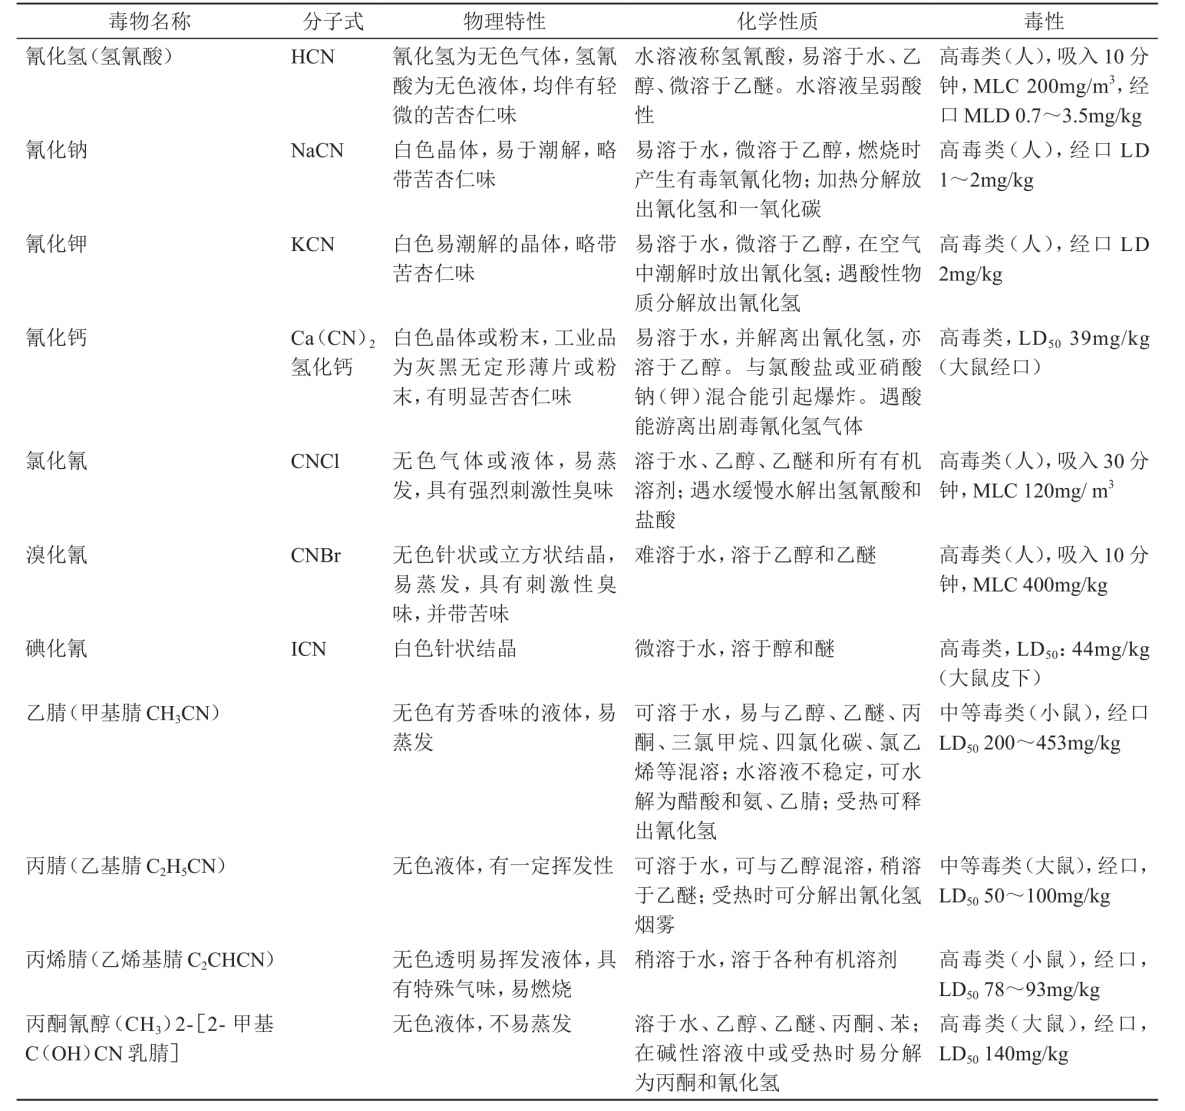
\includegraphics[width=6.69792in,height=6.27083in]{./images/Image00215.jpg}
\end{table}

\paragraph{前驱期(刺激期)}

吸入者可感眼、咽喉及上呼吸道刺激性不适,呼吸增快,呼出气有苦杏仁味,头昏、恶心。很快出现口腔、咽喉感觉障碍及麻木,尤以舌尖部更为显著,并有流泪、流涎、恶心、呕吐、头痛、乏力、耳鸣、胸闷及便意。一般此期短暂,不超过10分钟,如将患者迅速转移至新鲜空气处,上述症状可以消失。

\paragraph{呼吸困难期}

紧接上期出现胸部紧迫感、呼吸困难、心悸、血压升高、脉快、心律不齐,瞳孔先缩小后散大。眼球突出,视、听力减退,有恐怖感,意识模糊至昏迷,时有肢体痉挛,皮肤黏膜呈鲜红色。

\paragraph{惊厥期}

患者出现强直性或阵发性痉挛,甚至角弓反张,大小便失禁,大汗,血压下降,呼吸有暂停现象。

\paragraph{麻痹期}

全身肌肉松弛,感觉和反射消失,呼吸浅慢,甚至呼吸停止。若能抢救及时,可制止病情进展。

\subsection{治疗}

氰离子在体内易与三价铁结合,在硫氰酸酶参与下同硫结合成毒性很低的硫氰酸盐从尿排出,因此,高铁血红蛋白形成剂和供硫剂的联合应用可达到解毒的目的。急性中毒具体治疗措施有:

\paragraph{现场急救}

如系吸入中毒,立即戴上防毒面具,使患者迅速脱离中毒现场,如系液体染毒,立即脱去污染衣物,同时冲洗污染皮肤。呼吸停止者行人工呼吸,给予呼吸兴奋剂。

\paragraph{解毒药物的应用}

具体用药是:①立即将亚硝酸异戊酯1~2支放在手帕中压碎,放在患者口鼻前吸入15~30秒,间隔2~3分钟再吸1支,直至静脉注射亚硝酸钠为止(一般连续用5~6支);②在吸入亚硝酸异戊酯的同时,尽快准备好3\%亚硝酸钠注射液,按6~12mg/kg加入25\%~50\%葡萄糖液20~40ml中缓慢静注(2~3ml/min),注射时注意血压,一旦发现血压下降,立即停药。上述两药仅限于刚吞入毒物,现场抢救时有效;③在注射完亚硝酸钠后,随即用同一针头再注入50\%硫代硫酸钠(大苏打)20~40ml,必要时可在l小时后重复注射半量或全量,轻度中毒者单用此药即可。

上述疗法的作用在于亚硝酸盐能使血红蛋白氧化为高铁血红蛋白,后者对氰离子有很大的亲和力,结合成氰化高铁血红蛋白,从而有效地阻止氰离子对细胞色素氧化酶的作用,但此结合不牢固,不久又放出氰根,故应随即注射硫代硫酸钠,使其与氰形成稳定的硫氰酸盐,由尿排出体外。亚硝酸异戊酯和亚硝酸钠的作用相同,但后者作用较慢,维持时间较长,青光眼者慎用。本品用量过大产生变性血红蛋白过多可致缺氧,但同时应用硫代硫酸钠多能避免之。如无亚硝酸钠,可用大剂量亚甲蓝(10mg/kg)静注代替,但疗效较差。葡萄糖加少量胰岛素静滴可使氰离子转化为腈类而解毒。

4-二甲基氨基苯酚(4-DMAP)为一种新的高铁血红蛋白形成剂,其优点为具有迅速形成高铁血红蛋白的能力,抗氰效果优于亚硝酸钠,副作用轻,使用方便,可以肌肉注射,与静脉注射有相同的效果,而且可以口服,10分钟达到有效浓度。不但可用于治疗,也可用于预防。轻度中毒可口服1片4-DMAP,较重中毒立即肌注10\%
4-DMAP 2ml;重度中毒立即用10\% 4-DMAP
2ml肌注,50\%硫代硫酸钠20ml静注,必要时l小时后重复半量。应用本品者严禁再用亚硝酸类药物,以防止高铁血红蛋白形成过度症(发绀症)。

4-DMAP
3mg/kg和对氨基苯丙酮(PAPP)1.5mg/kg合用,可组成抗氰预防片,能有效预防氰化物中毒,口服40分钟显效,有效时间为4~6小时。

依地酸二钴的钴与氰离子结合形成无毒的氰化钴,其解毒作用快而强,无降压副作用,故为治疗本病的首选药物之一。其用法是600mg加入50\%葡萄糖40ml内,静脉缓慢注入。必要时,可重复应用8~10次。

\paragraph{洗胃}

如系口服中毒者,可用大量5\%硫代硫酸钠溶液或1∶5000高锰酸钾溶液或3\%过氧化氢溶液洗胃(忌用活性炭),以使胃内氰化物变为不活动的氰酸盐。洗胃后再给硫酸亚铁溶液,每10分钟1汤匙,可使氰化物生成无毒的亚铁氰化铁。由于氰化物吸收极快,故洗胃可在上述解毒剂应用后再进行。

\paragraph{高浓度给氧}

既往认为窒息性气体中毒机制是细胞呼吸酶失活,输氧无助于缺氧状态的改善。近来的研究证明,高流量吸氧可使氰化物与细胞色素氧化酶的结合逆传,并促进硫代硫酸钠与氰化物结合生成硫氰酸盐。有条件应尽早使用高压氧疗法。

\paragraph{对症支持疗法}

皮肤灼伤可用1∶5000高锰酸钾液擦洗或大量清水冲洗。恢复期可用大剂量维生素C,以使上述治疗中产生的高铁血红蛋白还原。亦可应用细胞色素C。

\protect\hypertarget{text00149.html}{}{}

\section{硫化氢中毒}

硫化氢(hydrogen sulfide,H\textsubscript{2}
S)为无色、带臭鸡蛋样气味的气体,在空气中燃烧呈蓝色火焰并生成二氧化硫。比重1.192,易溶于水。其水溶液呈酸性。多为工业生产中排放的废气,亦可由有机物腐败产生。因有机物腐败接触H\textsubscript{2}
S最多见于处理污水池、污水井、疏通阴沟、下水道、清掏粪窖和人工沼气池及挖掘河渠等作业,这些地方发生的中毒,有相当部分系由硫化氢引起。空气中H\textsubscript{2}
S浓度超过40mg/m\textsuperscript{3}
即有可能引起中毒症状;1000mg/m\textsuperscript{3}
经数秒钟即可引起人严重中毒;1400mg/m\textsuperscript{3}
可使人立即昏迷,呼吸麻痹死亡。

急性硫化氢中毒是短期内吸入较大量硫化氢气体后引起的以中枢神经系统、呼吸系统为主要靶器官的多器官损害的全身性疾病。据统计,1989~2003年间我国报告的重大急性中毒事故中,硫化氢所致的中毒事故起数(144起,占28.5\%)、中毒人数(677人,占14.5\%)、死亡人数(306人,占39.9\%)均排列在第1位;硫化氢中毒事件起数、中毒人数和死亡人数分别占窒息性气体总中毒起数的52.7\%、总中毒人数41.3\%和总死亡人数的50.3\%,均排在窒息性气体中毒的第1位;硫化氢中毒的中毒率和死亡率也较高,分别为84.2\%和44.6\%。

\subsection{病因与中毒机制}

H\textsubscript{2}
S是具有刺激性和窒息性的有害气体。接触低浓度仅有呼吸道及眼的局部刺激作用,此局部刺激作用是由于它接触湿润黏膜后形成硫化钠及其本身的酸性所致;高浓度时全身作用较明显,表现为中枢神经系统症状和窒息症状。急性中毒均由呼吸道吸入所致。H\textsubscript{2}
S进入人体后,在一定的剂量范围内,小部分可以原形或随呼出气排出,大部分则被氧化生成无毒的硫化物、硫代硫酸钠及硫酸盐等排出体外,在体内无蓄积作用。对机体产生危害的是来不及代谢和排出的游离H\textsubscript{2}
S,它进入血液后可先与高铁血红蛋白结合形成硫化高铁血红蛋白(H\textsubscript{2}
S并不直接与氧合血红蛋白结合,而是先由氧合血红蛋白变成高铁血红蛋白后,再与高铁血红蛋白结合而成硫化高铁血红蛋白),过量的未能结合的H\textsubscript{2}
S,即随血液进入组织细胞,发挥致毒作用。H\textsubscript{2}
S主要与呼吸链中细胞色素氧化酶及二硫链(-S-S-)起作用,影响细胞的氧化还原过程,造成组织细胞内窒息缺氧。如吸入H\textsubscript{2}
S浓度甚高时,强烈刺激颈动脉窦,反射性地引起呼吸停止;也可直接麻痹呼吸中枢而立即引起窒息造成闪电式中毒死亡。

\subsection{诊断}

\paragraph{病史}

有与H\textsubscript{2} S接触(如清理粪池、菜窖、阴沟等)史。

\paragraph{临床表现特点}

主要以中枢神经系统损害,眼和呼吸道刺激症状,以及心肌损害等中毒表现。急性H\textsubscript{2}
S中毒可分为以下三级:

\hypertarget{text00149.htmlux5cux23CHP5-4-3-2-2-1}{}
(1) 轻度中毒:

主要表现为眼和上呼吸道的刺激症状,如畏光、流泪、眼刺痛及异物感、流涕、鼻及咽喉灼热感、胸闷有紧束压迫感及刺激性干咳等。体检可见眼结膜充血,胸部听诊可有干啰音。一般于数日内症状消失。

\hypertarget{text00149.htmlux5cux23CHP5-4-3-2-2-2}{}
(2) 中度中毒:

除上述症状加重外,还有中枢神经系统的一般中毒症状(头痛、头晕、乏力等)及共济失调、消化系中毒症状(恶心、呕吐、肝肿大及功能障碍)。患者呼吸困难,呼出气体有臭鸡蛋样味;同时有视觉功能障碍,眼看光源时,可在光源周围见到彩色环,这是角膜水肿的征兆。

\hypertarget{text00149.htmlux5cux23CHP5-4-3-2-2-3}{}
(3) 重度中毒:

多为吸入高浓度H\textsubscript{2}
S引起。一般先有头痛、头晕、胸闷、心悸,继之谵妄、躁动不安、抽搐、意识障碍、昏迷。心肌损害有ST-T改变、各种类型的心律失常等。抽搐和昏迷可间歇发作。最后可因呼吸麻痹而死亡。昏迷时间较久者,同时可发生细支气管肺炎和肺水肿、脑水肿。吸入极高浓度(>
1000mg/m\textsuperscript{3}
以上)时,可立即猝死,即闪电式中毒。此为呼吸中枢麻痹所致,因为高浓度的H\textsubscript{2}
S可以麻痹嗅神经,由于嗅不出H\textsubscript{2}
S的腐败气味,故不能及时自动脱离有毒环境。严重中毒病例经抢救恢复后,部分患者可残留有后遗症,如神经衰弱症、前庭功能障碍、锥体外系损害、中毒性肾损害、精神障碍、痴呆、瘫痪及心血管病变等。

\subsection{治疗}

\paragraph{现场急救}

应立即将患者沿上风方向拖离现场,移至空气新鲜处,脱去被污染的衣物,保暖,吸氧。对呼吸心搏骤停者,立即进行心肺复苏术。应确保抢救者自身安全。

\paragraph{高压氧治疗}

高压氧治疗可有效地改善机体的缺氧状态,并可加速硫化氢的排出和氧化解毒。凡昏迷者,宜立即行高压氧治疗,每日1~2次,10~20次一疗程,一般用1~2个疗程。

\paragraph{对症支持治疗}

对躁动不安、高热昏迷者,可采用亚冬眠或冬眠疗法。宜早期、足量、短程应用糖皮质激素以及时防治中毒性肺水肿、脑水肿。换血疗法可以将失去活性的细胞色素氧化酶和各种酶及游离的硫化氢清除出去,故危重病例可考虑应用(换血量每次约500ml)。应用大剂量谷胱甘肽、半胱氨酸或胱氨酸等,以加强细胞的生物氧化能力,加速对硫化氢的解毒作用。同时给予改善细胞代谢的药物如细胞色素C等。眼部损伤者,尽快用清水或2\%碳酸氢钠溶液冲洗,继之用4\%硼酸水洗眼,再滴入无菌橄榄油和醋酸可的松点眼液,防止角膜炎的发生。用抗生素预防感染。

\paragraph{高铁血红蛋白形成剂的应用}

高铁血红蛋白形成剂能将血红蛋白氧化为高铁血红蛋白,使之与H\textsubscript{2}
S结合,减少其对细胞呼吸的毒性作用。但目前尚存在较大争议。一般认为,患者本来组织器官缺氧,如再加用亚硝酸钠或大剂量亚甲蓝(每次10~20mg/kg)等高铁血红蛋白形成剂,将使患者经受双重缺氧,会加重病情;硫化氢进入细胞与呼吸酶和其他活性物质的亲和力不是很强,可以较快的解离;再被游离出来的硫化氢又可被机体氧化解毒,硫化氢进入体内在有氧条件下很快被氧化,而且机体对硫化氢的代偿能力较强。因此多数学者认为应用高铁血红蛋白形成剂治疗虽然在理论上有依据,但临床疗效仍属可疑。但在重度硫化氢中毒患者中可考虑使用,可用药物有4-DMAP和3\%亚硝酸钠,具体用法见本章第2节“氰化物中毒”,但禁用硫代硫酸钠。大剂量亚甲蓝(每次10~20mg/kg)效果不理想,一般不主张应用。辅以静滴高渗葡萄糖和大剂量维生素C,有助于高铁血红蛋白还原。

\hypertarget{text00149.htmlux5cux23CHP5-4-3-4}{}
参 考 文 献

1. 陆再英,钟南山.内科学.第7版.北京:人民卫生出版社,2008:935

2. 任引津
,张寿林,倪为民,等.实用急性中毒全书.北京:人民卫生出版社,2003:111

3. 徐中杰
,刘梅,蔡振林.大剂量亚甲蓝抢救急性重度硫化氢中毒的临床研究.中国急救医学,2004,24(8):568

4. 黄汉林 .职业中毒应急处理.广州:中山大学出版社,2008:95

\protect\hypertarget{text00150.html}{}{}

\section{火灾烟雾中的有毒气体中毒}

火灾是最常见的灾害,人员伤亡大。我国每年约有3000多人死于火灾。统计结果表明,火灾中85\%以上的死亡者是由于烟雾的影响所致,其中大部分是吸入了烟尘及有毒气体窒息而致死的。随着新的建筑材料和装饰材料的不断出现,火灾烟雾中的有毒气体中除大量的一氧化碳和氰化氢外,氯气、氨气、二氧化硫、醛类、酚类以及氧化剂等有毒气体含量也很高,使火灾烟雾的毒性也大大增强。我国的统计资料表明,由于一氧化碳中毒窒息死亡或被其他有毒烟气熏死者占火灾总死亡人数的40\%~50\%,最高达65\%以上。而被烧死的人当中,多数是先中毒窒息后被烧死。因此开展对火灾烟雾毒性和中毒救治方法的研究具有现实意义。

\subsection{病因与发病机制}

火灾烟雾中毒见于各种火灾,包括居民楼、办公楼的火灾,化工厂原料燃烧、爆炸,烟花爆炸、燃烧等,特别是烟雾被限制在较小的空间且浓度较高时,人员中毒的可能性就越大,中毒程度也越严重。

几乎所有火灾都会产生大量的烟雾,烟雾是当材料热解或燃烧时产生的气溶胶颗粒、液体微滴和气体的混合物。燃烧产物中的不少组分是有毒的,再加上火灾烟雾的温度较高,因而烟雾已成为火灾中人员生命的最大威胁。每种可燃材料或制品热解或燃烧时可产生大量有毒的烟雾,当烟雾浓度足够高时就可对暴露的人员形成危害。烟雾对眼刺激造成视力减弱、吸入窒息性气体对上呼吸道和下呼吸道的刺激并反射性地引起昏迷。在火灾中这些效应常常同时发生,导致机体失能、行动的协调能力丧失、判断错误、方向知觉丧失、视力受限、疼痛,结果引起逃离火场迟缓或不能逃离,继之进一步吸入有毒气体或受到热烧伤,造成机体损伤甚至死亡。

\paragraph{一氧化碳(carbon monoxide,CO)}

CO是由含碳的化合物不完全燃烧所致,在所有的火灾中都有大量的CO产生。在火灾烟雾的各种成分中,CO是唯一被证实的能在火灾中可造成人员死亡的有毒气体。无论是无氧燃烧(闷烧)还是明火燃烧都可产生CO,前者是一个相当慢的过程,1~3小时才能达到致死的CO浓度,而转变到明火燃烧,这个时间相对较短。但在通风良好条件下,CO的产生一般很少。动物实验结果显示,浓度为2300~5700mg/m\textsuperscript{3}
的CO能使受试小白鼠全部死亡,对人来说,11 000~12
000mg/m\textsuperscript{3} 浓度的CO就可使人很快停止呼吸而死亡。

CO本身对组织细胞并无明显毒性,其引起机体中毒的原因在于同血红蛋白(Hb)结合后形成COHb,从而使血液携氧能力降低而造成组织缺氧,而动脉血氧分压和血流量是正常的。CO与Hb亚铁血红素结合位点有很强的亲和力,当吸入空气中含有20.9\%的氧气(O\textsubscript{2}
)和0.07\%的CO时,血液中形成COHb和HbO\textsubscript{2}
的量基本相等,即CO 与Hb的亲和力比O\textsubscript{2}
大300倍,所以即使吸入的空气中存在少量的CO,亦能形成大量的CO而造成全身缺氧。另外CO对二价铁的高度亲和力,使它可与细胞内还原型细胞色素氧化酶结合,直接抑制细胞呼吸。但血液循环中已有大量含有二价铁的血红蛋白存在,故一般情况下,进入体内的CO绝大多数已与血红蛋白结合,不致进入细胞中去,除非高浓度的短期大量吸入,CO的这种细胞呼吸抑制作用才具有一些临床意义。实验证明,由于进入细胞内的CO太少,CO对细胞呼吸抑制作用不明显。

\paragraph{氢氰酸(hydrocyanic acid,HCN)}

许多现代的塑料家饰材料热降解时可产生大量HCN气体,在火灾死亡者中也发现其血{[}CN{]}浓度增高。火灾中HCN的产生与可燃物的材料和燃烧温度均有关,理论上只要是含氮的材料在相对较高的温度下就可产生HCN。不同的含氮材料,有天然的如羊毛和丝绸,人工合成的如聚亚胺酯和聚丙烯腈,在热分解时都可产生中毒浓度的HCN。在一个5.6L的燃烧室内热解1g聚丙烯腈,产生的HCN浓度为1500ppm;在一个中等大小的客厅内燃烧2kg聚丙烯腈产生的HCN可达到致死浓度。动物实验结果显示,100~120mg/m\textsuperscript{3}
浓度的HCN气体就能使受试大白鼠全部致死。实验中动物吸入含有HCN的烟雾可迅速出现严重的失能,许多火灾受害者是由于不能从火中逃生,烟雾产生的视力模糊、眼睛刺激、呼吸困难阻碍了受害者的逃生。失能可能是由HCN中毒引起,耽误了火灾受害者逃生能力,延长有毒气体吸入或被火烧伤的时间,因此大大增加了死亡或损伤的可能性。

HCN的毒性比CO大25倍以上,而且作用迅速。与CO主要存在于血液中不同,火灾烟雾中HCN主要通过呼吸道进入人体,之后迅速离解出CN离子,并弥散到全身的体液,与组织、器官的细胞接触。CN离子可与细胞线粒体上的氧化呼吸链中氧化型细胞色素氧化酶的辅基铁卟啉的F\textsuperscript{3+}
迅速牢固结合,阻止其还原成F\textsuperscript{2+}
,中断细胞色素aa\textsubscript{3}
至氧的电子传递,使生物氧化过程受抑。虽然血液为氧所饱和,但不能被组织细胞摄取和利用,引起细胞内窒息。与CO相比,CN并没有降低组织的供氧,而是抑制了细胞利用氧的能力。心脏和脑组织对细胞呼吸抑制尤其敏感,HCN中毒引起的死亡通常是由于中枢性呼吸抑制所致。文献报道,在HCN浓度为50ppm的空气中人可耐受0.5~1.0小时,但在HCN浓度为100ppm的空气中暴露同样时间则可能致命;130ppm在30分钟后死亡,180ppm暴露10分钟就可致死。

因游离的血CN在体内的半衰期很短,约1小时,所以在火灾幸存者中测得的血{[}CN{]}往往要低于初始暴露吸入的浓度。一般认为HCN吸入后,血{[}CN{]}>
1.0μg/ml就可能出现明显的毒理作用,{[}CN{]}>
3.0μg/ml被认为是致死的。在一些火灾中HCN中毒已超越CO中毒成为致死的主要因素,表现为火灾死亡者血{[}CN{]}已达到致死水平,但COHb\%却未达到中毒浓度。在一次聚亚酯床垫的燃烧引起的火灾事故中,死亡的35人血液检测发现大多数死者的血{[}CN{]}为2~4μg/ml,COHb\%为5\%~10\%,表明含有致死量{[}CN{]}和仅仅低浓度的COHb,烟雾中HCN吸入中毒是这次火灾大量人员死亡的主要原因。

CO和HCN这两种有毒气体在毒性效应上有累加作用。火灾烟雾中毒者血中常可同时检测到{[}CN{]}和COHb\%升高。有报道美国在43次飞机失事火灾中死亡的73人血中测得COHb\%(>
10\%)和{[}CN{]}(>
0.25μg/ml)浓度超过标准,而在非火灾致死者中均未超过标准。由火灾致死的血中两种气体的浓度范围都可引起中等程度的中毒反应,但均未达到致死浓度,非致死浓度的CO和HCN中毒作用累加,产生了致死效应。在有HCN吸入中毒的火灾死亡者中COHb含量通常低于50\%,表明HCN对CO吸收有抑制作用。动物实验表明,当CO浓度升高时,动物氰化物中毒LD\textsubscript{50}
降低。因HCN、CO复合中毒对机体缺氧的程度有协同效应。在没有或只有轻微烧伤的火灾受害者中,除了考虑CO中毒外,还应想到有HCN中毒的可能。

\paragraph{二氧化碳(carbon dioxide,CO\textsubscript{2} )}

CO\textsubscript{2}
本身毒性相当低,但可使吸入气中氧的成分降低,降低血液的运输氧的能力。CO\textsubscript{2}
的LC\textsubscript{50} 是470
000ppm(47\%),在实际的火灾中不可能达到这个浓度的,火灾中如果所有的O\textsubscript{2}
都转变成CO\textsubscript{2}
,其最大浓度也只有21\%左右。CO\textsubscript{2}
和CO之间有协同效应,一般在火灾中的CO\textsubscript{2}
的浓度为5\%,但可使CO的毒性增加50\%;当浓度超过5\%时,CO的毒性又回到其本身的毒性。这是由于CO\textsubscript{2}
刺激呼吸的频率和深度,使每分钟通气量(RMV)增加所致。CO\textsubscript{2}
浓度为2\%时可使RMV增加约50\%。

\paragraph{氮氧化物}

氮氧化物主要是NO\textsubscript{2}
和NO的混合物,含氮材料(可燃物)在氧气充足时也会燃烧产生低浓度的氮氧化物,但其产生速度远比HCN慢。NO\textsubscript{2}
毒性是NO
的5倍,它是一种刺激性气体,可引起流泪、咳嗽、呼吸困难、肺水肿;NO\textsubscript{2}
气体与水反应,形成硝酸和亚硝酸可引起肺损伤。NO\textsubscript{2}
的LC\textsubscript{50} 约为200ppm,与HCN的LC\textsubscript{50}
相似。但与HCN相比,氮氧化物的致死效应主要是肺刺激效应,死亡时间也在中毒后1天左右。在5\%
CO\textsubscript{2} 存在时,NO\textsubscript{2} 的LC\textsubscript{50}
变成90ppm。NO\textsubscript{2}
与HCN之间有相互作用,在30分钟LC\textsubscript{50}
浓度的NO\textsubscript{2} (200ppm)存在时,HCN的LC\textsubscript{50}
从200ppm增至480ppm,表明NO\textsubscript{2}
对HCN有拮抗作用,这可能是因为NO\textsubscript{2}
可使血红蛋白转变成高铁血红蛋白(MetHb)。

\paragraph{其他刺激性气体}

刺激效应在所有的火灾烟雾中都存在,分为两类:一是感觉器官受刺激,包括眼、上呼吸道刺激症状;二是肺刺激症状。绝大多数的火灾烟雾二种刺激效应是共存的。PVC塑料分解时可产生HCl,这种酸性气体既是一种强的感官刺激剂,也是一种强的肺组织刺激剂,75~100ppm的浓度就可引起眼和上呼吸道的剧烈刺激。在火灾中也会产生许多有机刺激物,主要是丙烯醛,对眼和上呼吸道都有刺激作用。

\subsection{诊断}

\subsubsection{临床表现特点}

在火场中,凡是出现头晕、乏力、流泪、咳嗽、胸闷、呼吸困难等症状,即是中毒的先兆,如果持续下去就有可能发生中毒昏迷甚至死亡。一般来说,轻度中毒只有先兆症状,只要及时撤离现场,到有新鲜空气处休息,短时间内可自行缓解;中度中毒除有先兆症状外,尚有全身反应,如:心悸、气短、呼吸困难、不能站立、肌肉痉挛、恶心、呕吐、畏冷、面色苍白或变紫青色,等等;重度中毒者常伴有神志不清、昏迷或呼吸心跳停止。

\subsubsection{实验室检查}

\paragraph{痰液检查}

早期痰液中烟尘、细菌的检查有助于肺炎的诊断和治疗。

\paragraph{碳氧血红蛋白}

多数伤员血中碳氧血红蛋白在10\%~50\%,但在停止烟雾吸入之后可发生解离,尤其在给予高浓度氧吸入后明显降低,这往往会使医师低估中毒的严重程度。

\paragraph{X线检查}

对烟雾吸入中毒者的早期诊断意义较小,大部分患者胸部X线片无异常。48小时后少数患者出现肺泡和间质水肿、局限性浸润,一般数日消失,部分有肺炎表现。

\subsubsection{诊断注意事项}

有毒气体中毒的临床严重程度差别很大,轻者可无明显症状和体征。而严重的有毒气体吸入中毒,可迅速并发急性肺功能衰竭,因此应尽快明确诊断。早期诊断在于综合分析临床资料、实验室检查、X线和特殊检查的结果。

\subsection{治疗}

在火灾烟雾有毒气体中,除了CO和HCN能引起急性中毒致死外,其他的气体主要对眼和上呼吸道有刺激效应,脱离火场后对患者进行对症处理即可,因此火灾烟雾中毒患者救治主要是针对CO和HCN中毒的急救。对火灾烟雾吸入中毒者在给予初步的生命支持处理包括高浓度吸氧,还应紧急测血气、COHb、高铁血红蛋白、{[}CN{]}和乳酸。如果患者一直持续昏迷、惊厥、心律不齐、酸中毒和低血压,尤其是血浆乳酸浓度高于10mmol/L,且无其他因素引起乳酸升高,提示有HCN中毒,应给予抗氰治疗。

单独的CO和HCN中毒的都有传统的急救方案,且救治效价高。吸氧或高压氧治疗是目前CO中毒首选的救治方法,疗效可靠。HCN吸入中毒经典的抗氰急救方法是用亚硝酸异戊酯和亚硝酸钠促使高铁血红蛋白形成,与血液中的CN结合。硫代硫酸盐在线粒体促使CN转变为硫氰酸盐,并给予氧气吸入以提高抗氰治疗效果。目前国内还常用对二甲氨基苯酚(4-DMAP)作为急救用药。在美国有一种称为Lilly的抗氰急救盒,内有12支亚硝酸异戊酯供吸入,300mg亚硝酸钠和12.5g硫代硫酸钠各2支,可静脉使用,临床医师可根据情况选用不同的抗氰剂。

但火灾烟雾中毒都是HCN和CO复合中毒,在这种情况下再用高铁血红蛋白形成剂亚硝酸盐类或4-DMAP作为抗氰急救用药有潜在的危险。因高铁血红蛋白形成剂是以牺牲血液的携氧能力为代价的,在正常情况下,30\%的血红蛋白形成高铁血红蛋白不致影响血液供氧。可是在烟雾吸入中毒情况下,对于已有大量血红蛋白与CO结合的中毒者来说,再形成高铁血红蛋白与CN结合,使血液的携氧能力进一步降低,可能就将危及生命。该药还能扩张血管、降低血压,对中毒合并出血和休克的伤员的急救也不利。因而在火灾烟雾HCN和CO复合中毒时,不能采用传统的抗氰急救方法,应尽量避免使用高铁血红蛋白形成剂类的药物。

除了高铁血红蛋白形成剂外,也有几类具有抗氰作用的药物,如供硫剂、钴制剂、醛酮化合物等。硫代硫酸钠属于供硫剂,也是经典的抗氰治疗中的药物,与亚硝酸盐配合使用以提高抗氰效价。但硫代硫酸钠的抗氰原理是促进体内的生化解毒途径,在硫氧生成酶作用下使CN氧化生成无毒硫氰酸盐(SCN),起效慢,用量大,且不能通过细胞膜进入细胞内,而绝大部分CN-位于细胞内。所以单独使用时,抗氰作用有限。

钴制剂和醛酮化合物都能和CN结合形成无毒的化合物。钴制剂的代表有依地酸钴和羟钴胺,依地酸钴作为北约的军用抗氰急救药,对濒死中毒者效果很好,但对轻、中度中毒者钴离子的毒副作用大。羟钴胺是维生素B\textsubscript{12}
的一种,毒性较小,且与CN的结合速度快,作用强,被认为是一个有效、安全和给药容易的抗氰剂,在可疑氰化物中毒时适于院外使用。羟钴胺已在美国进入临床试验,一旦成功,可避免在火灾烟雾吸入中毒患者中使用亚硝酸钠的副作用,对严重烟雾吸入中毒者可给予羟钴胺。在醛酮化合物中二羟丙酮(DHA)与硫代硫酸钠合用有较好的抗氰效价,且DHA是细胞糖酵解过程的中间产物,在火灾烟雾吸入已形成COHb造成血液携氧能力下降的情况下,DHA可作为亚硝酸钠的有效替代品。但羟钴胺和二羟丙酮目前仅停留在科研阶段,还未进入临床作为正式的抗氰药物。

吸氧在当今抗氰治疗中已不是作为一种辅助治疗手段,而是当作一种必不可少的救治药物和方法。氧气单独使用时也具有一定的抗氰能力,可提高抗氰药物的抗氰效价,但其抗氰机制还不是很清楚。氧气对CO和HCN中毒治疗都有益,吸氧或是有条件的话使用高压氧舱是CO中毒的首选治疗方法。氧有一定的抗氰能力,且氧疗本身没什么副作用,因此氧疗已成为火灾烟雾吸入中毒患者的一个基本治疗手段。

\protect\hypertarget{text00151.html}{}{}

\chapter{有机毒物中毒}

\section{急性乙醇中毒}

急性乙醇(酒精)中毒(acute ethanol
poisoning),俗称酒醉,系由一次饮入过量乙醇(酒精)或酒类饮料引起的中枢神经系统由兴奋转为抑制的状态,严重者出现昏迷、呼吸抑制及休克。

\subsection{病因与中毒机制}

各种酒类饮料中含有不同浓度的乙醇:一般黄酒含10\%~15\%、白酒含50\%~60\%、果酒16\%~48\%、啤酒2\%~5\%。成人饮用乙醇的中毒剂量有个体差异,一般为70~80g,而致死剂量为250~500g。小儿的耐受性较低,致死量婴儿6~10g,儿童约25g。许多毒物如汞、砷、硝基苯等使人体对乙醇的耐受性下降,反之酒后对上述毒物的感受性也增加。在32℃高温条件下,乙醇的毒性可提高1~2倍。饮入的乙醇80\%由小肠上段吸收,其余由胃吸收。空腹饮酒时,在1小时内有60\%被吸收,2小时吸收量已达95\%。胃内有食物存在,可延缓乙醇的吸收。乙醇被吸收后,通过血流遍及全身,约90\%在肝脏由乙醇脱氢酶和过氧化氢酶氧化为乙醛,由醛脱氢酶进一步氧化为乙酸,最后经三羧酸循环氧化为CO\textsubscript{2}
和水。约2\%乙醇不经氧化而缓慢经肺、肾排出。

乙醇的急性毒害作用有:①中枢神经系统抑制作用:乙醇对中枢神经系统的抑制作用,随着剂量的增加,由大脑皮质向下,通过边缘系统、小脑、网状结构到延髓。小剂量出现兴奋作用,这是由于乙醇作用于大脑,细胞突触后膜苯二氮{}
-GABA受体,从而抑制GABA对脑的抑制作用。随着乙醇血中浓度增高,作用于边缘系统、小脑,患者表现为步态蹒跚、共济失调等运动障碍,继而功能抑制出现精神失常;作用于脑干网状结构,引起昏睡或昏迷;最后由于抑制延髓血管运动中枢和呼吸中枢出现休克、呼吸衰竭,呼吸中枢麻痹是致死的主要原因。此外,由于血管扩张及缺氧可导致脑水肿。②代谢异常:乙醇在肝细胞内代谢生成大量还原型烟酰胺腺嘌呤二核苷酸(NADH),使之与氧化型的比值(NADH/NAD)增高,可高达正常的2~3倍,相继发生乳酸增高、酮体蓄积导致的代谢性酸中毒以及糖异生受阻所致低血糖。饮酒发生的低血糖多见于嗜酒者,在无肝脏病者或营养良好的人也可能发生,此时血糖浓度降低是由于肝脏葡萄糖异生减弱、释放葡萄糖减少所致;糖异生受抑制是由于肝脏NADH/NAD的比例增加所致。NADH/NAD比值上升,使肝脏中乳酸的利用降低,另一方面丙酮酸被NADH还原成乳酸,易发生乳酸性酸中毒。

此外,过量饮酒可诱发消化道出血、胰腺炎、发作性心律失常、脑梗死、脑出血及蛛网膜下腔出血,个别可引起急性乙醇中毒性肌病(肌痛、肌无力、肌肉肿胀,横纹肌溶解而导致急性肾功能衰竭)。

\subsection{诊断}

\paragraph{饮酒史}

有过量饮酒史,应询问饮酒的种类和饮用量、平素酒量、饮酒的具体时间,有无服用其他药物。

\paragraph{临床表现特点}

一次大量饮酒中毒可引起中枢神经系统抑制,症状轻重与饮酒量、血中乙醇浓度、个体的耐受性有关。临床上大致分三期,各期界限不很明显。

\hypertarget{text00151.htmlux5cux23CHP5-5-1-2-2-1}{}
(1) 兴奋期:

当饮酒后,血中乙醇浓度达到11mmol/L
(50mg/dl)时,即感头痛、欣快、兴奋。血中乙醇浓度超过16mmol/L(75mg/dl)时,健谈、饶舌、情绪不稳定、自负、易激怒,可有粗鲁行为或攻击行动,也可能沉默、孤僻。血中乙醇浓度达到22mmol/L(100mg/dl)时,驾车易发生车祸。

\hypertarget{text00151.htmlux5cux23CHP5-5-1-2-2-2}{}
(2) 共济失调期:

血中乙醇浓度达到33mmol/L(150mg/dl)时,即可出现共济失调,表现为动作笨拙,步态蹒跚,语无伦次,且言语含糊不清。血乙醇浓度达到43mmol/L(200mg/dl)时,出现恶心、呕吐、困倦。

\hypertarget{text00151.htmlux5cux23CHP5-5-1-2-2-3}{}
(3) 意识障碍期:

血中乙醇浓度达到54mmol/L(250mg/dl)时,即转入昏睡状态,面色苍白或潮红,皮肤湿冷、口唇轻度发绀、心跳加快,呈休克状态。瞳孔散大,呼吸缓慢带鼾声,严重者大小便失禁、抽搐、昏迷,最后发生呼吸麻痹直至死亡。

患者呼出气及呕吐物均有酒味。小儿饮中毒量乙醇后,很快进入沉睡,不省人事,一般无兴奋过程。由于严重低血糖,可发生惊厥,亦可发生高热、休克、吸入性肺炎和颅内压升高等。老年人肝脏功能相对较差,如饮用等剂量的酒,血中乙醇浓度较青壮年人高,故症状较重,死亡率亦高。

\paragraph{戒断综合征}

长期酗酒者在突然停止饮酒或减少酒量后,可发生下列4种类型戒断综合征的反应:①单纯性戒断反应:在减少饮酒后6~24小时发病。出现震颤、焦虑不安、兴奋、失眠、心动过速、血压升高、大量出汗、恶心、呕吐。多在2~5天内缓解自愈。②酒精性幻觉:幻觉以幻听为主,也可见幻视、错觉及视物变形。多为被害妄想,一般可持续3~4周后缓解。③戒断性惊厥反应:常与单纯性戒断反应同时发生,也可在其后发生癫痫大发作。多数只发作1~2次,每次数分钟。也可数日内多次发作。④震颤谵妄反应:在停止饮酒24~72小时后,也可在7~10小时后发生。患者精神错乱,全身肌肉出现粗大震颤。谵妄是在意识模糊的情况下出现生动、恐惧的幻视,可有大量出汗、心动过速、血压升高等交感神经兴奋的表现。

\paragraph{实验室检查}

依病情查血电解质、血糖、淀粉酶、肌酸磷酸激酶、血气分析等。

\paragraph{诊断注意事项}

①需检查患者有无摔倒或碰撞致外伤,尤其是颅脑外伤致颅内出血引起意识障碍。②下列情况需行颅脑CT检查:经治疗意识未恢复或意识状态发生改变;出现定位体征;饮酒量与临床表现不符;癫痫发作;有外伤史。③急性中毒主要与引起昏迷的疾病相鉴别,如镇静催眠药中毒、CO中毒、急性脑血管病、糖尿病昏迷、颅脑外伤等。④戒断综合征主要与精神病、癫痫、窒息性气体中毒、低血糖症等相鉴别。

\subsection{治疗}

\paragraph{急性中毒的治疗}

急性中毒的轻型患者,一般无需特殊治疗。可使其卧床休息、保暖、饮浓茶或咖啡,即可逐渐恢复。患者昏睡或昏迷时应注意保暖、侧卧位,保持呼吸道通畅,及时清理呕吐物,以防误吸及窒息。对重症患者应迅速采取下述救治措施:

\hypertarget{text00151.htmlux5cux23CHP5-5-1-3-1-1}{}
(1) 清除毒物:

由于乙醇吸收快,一般洗胃意义不大;如在2小时内的重度中毒患者,可考虑应用1\%碳酸氢钠或生理盐水洗胃。对昏迷时间长、呼吸抑制、休克的严重病例,或血中乙醇浓度超过108mmol/L(500mg/dl),伴酸中毒或同时服用甲醇或其他可疑药物时,应尽早行血液透析治疗,可成功挽救患者生命。

\hypertarget{text00151.htmlux5cux23CHP5-5-1-3-1-2}{}
(2) 纳洛酮的应用:

纳洛酮对乙醇中毒所致的意识障碍、呼吸抑制、休克有较好的疗效。用法:0.4~0.8mg加入25\%葡萄糖液20ml中静注,必要时15~30分钟重复1次;或用1.2~2mg加入5\%~10\%葡萄糖液中持续静滴,直至达到满意效果。

亦可选用醒脑静注射液和胞磷胆碱治疗重度乙醇中毒。成人为醒脑静注射液20ml加入5\%~10\%葡萄糖溶液250ml中静滴;胞磷胆碱0.5~1g加入5\%~10\%葡萄糖溶液500ml中静滴。

\hypertarget{text00151.htmlux5cux23CHP5-5-1-3-1-3}{}
(3) 促进乙醇氧化代谢:

可给50\%葡萄糖液100ml静注,同时肌注维生素B\textsubscript{1}
、维生素B\textsubscript{6} 和烟酸各100mg,以加速乙醇在体内氧化代谢。

\hypertarget{text00151.htmlux5cux23CHP5-5-1-3-1-4}{}
(4) 对症支持疗法:

①维持呼吸功能:吸氧,畅通呼吸道,防治呼吸衰竭。②防治酸中毒:补充血容量,早期纠正乳酸性酸中毒,初剂量先给予5\%碳酸氢钠液150ml静滴,其后可根据血气分析结果补碱。必要时给予血管活性药物如多巴胺等。③防治脑水肿:可选用20\%甘露醇液125~250ml,50\%葡萄糖液60ml,地塞米松5~10mg静注。可按病情需要和血压情况,4~6小时后重复应用。④迅速纠治低血糖:部分病例可出现低血糖昏迷,应注意与乙醇直接作用所致的昏迷鉴别。故急性中毒的重症患者应检测血糖,如有低血糖,应立即静注高渗葡萄糖液。⑤镇静剂的应用:应慎用。对躁动不安、过度兴奋的患者,可用地西泮(安定)5~10mg肌注或静注,或氯丙嗪25~50mg肌注,或水合氯醛0.5~1.0g口服或保留灌肠。给药后注意病情变化。禁用吗啡及巴比妥类药物。⑥预防感染:昏迷患者可预防性应用抗生素。

\paragraph{戒断综合征的治疗}

患者应安静休息,保证睡眠。加强营养,给予维生素B\textsubscript{1}
、维生素B\textsubscript{2}
。有低血糖时静注高渗葡萄糖液。重症患者宜选用短效镇静药控制症状,常选用地西泮,依病情每1~2小时口服5~10mg,症状稳定后可给予维持镇静的剂量,8~12小时一次。有癫痫病史者可用苯妥英钠。

\protect\hypertarget{text00152.html}{}{}

\section{甲醇中毒}

甲醇(methyl
alcohol)又名木醇或木酒精,系无色、透明、易燃、易挥发、略带酒精气味的液体。比重0.79,蒸气比重1.11。易溶于水及多种有机溶剂。在工业上作为甲醛、塑料、胶片等的生产原料,并用于防冻剂及溶剂等。工业生产中急性中毒主要由吸入甲醇蒸气所致,较少见。工业用酒精中含有较多的甲醇,若误用此类酒精配制成白酒饮用,则导致急性中毒。

\subsection{病因与中毒机制}

甲醇主要经呼吸道及消化道吸收,皮肤也可部分吸收,吸收后迅速分布于各组织器官,含量与该组织器官的含水量成正比。甲醇在体内氧化及排出均缓慢,故有明显的蓄积作用。未被氧化的甲醇,主要经肺呼吸排出(约为进入量的14\%),也可经肾(约为进入量的30\%)排出,尚有小部分可由胃肠道缓慢排出。人经口中毒的个体差异较大,一般5~10ml即可引起严重中毒,最低7~8ml即可引起失明,致死量30ml左右。中毒的后果不一致,有的口服20ml余致死;15ml导致永久性失明,但也有口服250ml而获救存活者。其中毒机制主要为甲醇的氧化产物新生态甲醛或甲酸盐与细胞内的蛋白质相结合所致,对机体的危害主要有:①对中枢神经系统有明显的麻醉作用。其麻醉作用虽较乙醇为弱,但由于它氧化代谢缓慢,蓄积性强,故毒害作用远较乙醇为大;其麻醉浓度与致死浓度较为接近,故危险性也较大。②对视神经及视网膜有特殊的选择作用。眼房水和玻璃体含水量达99\%以上,甲醇能溶入水并和眼球组织有特殊亲和力,故中毒后眼球中甲醇含量高。甲醇经醇脱氢酶氧化而生成的甲醛,毒性较甲醇大约33倍,它作用于视网膜上的糖原酵解酶,使细胞线粒体受损伤,细胞色素氧化酶被抑制,从而抑制视网膜的氧化磷酸化过程,使膜内不能生成ATP,致使细胞发生退行性变,招致视网膜及视神经病变,最终导致视神经萎缩。此外,甲醇代谢所形成的甲酸,比甲醇毒性约大6倍,它可抑制某些氧化酶,并引起酸中毒;甲酸盐尚可致神经轴浆流障碍,也是使视网膜病变加剧的因素。③代谢性酸中毒。甲酸在体内的积累,再加上甲醇在体内可抑制某些氧化酶系统,使糖的需氧分解及机体代谢发生障碍,导致乳酸及其他有机酸在体内积聚,引起代谢性酸中毒。

甲醇或其氧化产物直接损害组织,其损害程度与该组织器官的含水量成正比。以下各器官组织的敏感性递减:眼、脑灰质、胃肠道、肺、肾、肝、胰。甲醇中毒主要病理损害为脑水肿、脑膜出血,视神经和视网膜萎缩性失明,肺部充血、水肿,肝、肾混浊肿胀等。

\subsection{诊断}

\paragraph{病史}

有接触甲醇、吸入甲醇蒸气、误服甲醇或饮入大量含有甲醇的劣质酒或假酒史。

\paragraph{临床表现特点}

主要引起以中枢神经系统损害、眼部损害和代谢性酸中毒为特点的中毒症状。

无论吸入或经口中毒,均有一定的潜伏期,通常为8~36小时,同时饮酒者则潜伏期可更长。症状轻者仅感头痛、头晕、视物模糊、乏力、兴奋、失眠、眼球疼痛,颇似乙醇中毒。中度中毒可出现步态不稳、呕吐、呃逆、共济失调,腹痛、腰痛、视力障碍、眼前有跳动性黑点、飞雪或闪光感,复视甚至视觉丧失,表情淡漠、四肢湿冷。重度中毒有剧烈头痛、恶心、呕吐,意识蒙眬、谵妄、抽搐、失明、瞳孔散大、光反射消失等表现。同时,患者有明显的酸中毒,甚至休克、昏迷,最后可出现中枢性呼吸衰竭而致死。少数病例可出现精神症状。个别患者可并发急性胰腺炎、周围神经病变或坐骨神经痛。

眼底检查见视神经乳头充血、出血或眼底静脉扩张、视网膜水肿,或见视神经萎缩。也有病例眼损害症状出现于全身中毒症状改善之后,由此可于中毒后数月出现迟发性视力损害。

\paragraph{辅助检查}

血气分析有HCO\textsubscript{3} \textsuperscript{−}
及pH降低,BE为负值。血CO\textsubscript{2}
CP降低。血和尿中酮体可阳性,尿呈酸性,可能有肝功能异常及蛋白尿。血和尿中可测得甲醇、甲酸含量增高。CT检查发现脑壳核梗死,同样有助于诊断。

\subsection{治疗}

1.早清除毒物
口服中毒者应及时用1\%~3\%碳酸氢钠或温水、肥皂水洗胃,口服硫酸钠30g导泻。已吸收入血液者,不论患者有无症状,均可用腹膜或血液透析加以清除,因甲醇属可透析清除的毒物。早期透析可减轻症状、挽救生命和减少后遗症。血液透析的指征为:①血液甲醇>
15.6mmol/L或甲酸>
4.34mmol/L;②严重代谢性酸中毒;③视力严重障碍或视乳头视网膜水肿。吸入性中毒应脱离有毒环境,吸氧。

2.乙醇作抗毒治疗
由于乙醇对醇脱氢酶的亲和力比甲醇大20倍,由此可阻断甲醇代谢增毒,并促进排出,如血液中乙醇浓度达到21~32mmol/L的水平,可完全抑制其代谢作用,故理论上可用乙醇作抗毒治疗。方法是医用95\%乙醇按1ml/kg稀释于5\%葡萄糖或生理盐水中,配制成10\%的乙醇溶液,30分钟内静滴完,然后再按0.166ml/kg同样稀释后静滴维持;也可先用50\%乙醇按1.5ml/kg稀释至不大于5\%的浓度,首次口服或经胃管注入,其后按0.5~1ml/kg口服,每2小时l次维持。也可口服白酒30ml,以后每4小时口服15ml。务使血中甲醇浓度降至0.5g/L以下,停止使用乙醇后不再发生酸中毒为止,一般约需4~7天或更长。若患者已有明显抑制者不宜用乙醇治疗。尚可给予叶酸,以促进已经形成的甲酸加速分解成CO\textsubscript{2}
,剂量为每4小时50mg静滴,共给数日。

4-甲基吡唑(4-methylpyrazole)是对醇脱氢酶有更强、更特异的抑制剂,且毒性低,有望取代乙醇作为甲醇或乙二醇的解毒剂。按15mg/kg口服1次,12小时后给5mg/kg,再12小时给10mg/kg,直至血中检测不出甲醇为止。

3.纠正酸中毒
早期应用碱性药物有肯定的疗效。可用5\%碳酸氢钠静滴,用量可根据血CO\textsubscript{2}
CP或血气分析结果调整。

4.高压氧治疗
重度中毒和有双目失明者,应尽早行高压氧舱治疗,可使双目失明好转。

5.肾上腺皮质激素
皮质激素可减轻脑水肿和视神经损害,可用地塞米松10~20mg或氢化可的松200~500mg静滴,每日1次。

6.眼科治疗
不论患者视力如何,急性期均宜避免光线刺激,双眼应用纱布覆盖保护。并可酌情用维生素B\textsubscript{1}
、维生素B\textsubscript{12} 和尼莫地平等,防止视神经发生永久病变。

7.对症支持疗法
给予高蛋白、高碳水化合物饮食。应用大剂量维生素及促进神经系统恢复的药物。

\protect\hypertarget{text00153.html}{}{}

\section{苯中毒}

苯(benzene)是从煤焦油分馏及石油裂解所得的一种芳香烃化合物,系无色有芳香气味的油状液体。挥发甚速,易燃易爆。是工业上广泛应用的溶剂和原料。急性中毒多由于生产过程或意外事件中吸入高浓度苯蒸气所引起。一般吸入含苯浓度4~5g/m\textsuperscript{3}
的空气,则会发生严重中毒。偶尔亦可因误服而中毒,口服2ml即可迅速发生昏迷,10~15ml可致死。

\subsection{病因与中毒机制}

苯主要以蒸气形态经呼吸道吸入,皮肤仅少量吸收,消化道吸收完全。进入体内后,部分以原形由肺呼出;部分在肝脏代谢,通过微粒体混合功能氧化酶进行羟化,转化为酚、对苯二酚、邻苯二酚等酚类代谢产物。这些代谢物分别与硫酸根、葡萄糖醛酸结合为苯基硫酸酯及苯基葡萄糖醛酸酯,自肾排出。急性中毒是因苯的亲脂性很强,且多聚集于细胞膜内,使细胞膜的脂质双层结构肿胀,影响细胞膜蛋白功能,干扰细胞膜的脂质和磷脂代谢,抑制细胞膜的氧化还原功能,致中枢神经系统麻醉。慢性毒作用主要是苯及代谢产物酚类所致造血系统损害:①酚类为原浆毒,直接抑制细胞核分裂,对增殖活跃的骨髓造血细胞,尤其是处于S及G\textsubscript{2}
期细胞有明显抑制作用;②酚类与巯基作用及与白细胞中硫结合,分别使谷胱甘肽代谢障碍及形成具有自身抗原性的变性蛋白,导致血细胞破坏;③苯也可抑制δ-氨基-γ-酮戊酸合成酶,干扰红细胞生成素对红细胞增殖的刺激作用。

\subsection{诊断}

\paragraph{病史}

有毒物接触史。由于吸入的苯部分以原形由呼吸道排出,中毒者气息中有浓郁的苯的芳香味,对无明确接触史者,有参考诊断价值。除苯的中毒外,口服中毒者,尚需注意服入作为溶剂的苯之外,是否尚有作为溶质的其他毒物进入体内,招致“双重中毒”的可能性。

\paragraph{临床表现特点}

急性中毒主要为中枢神经系统抑制症状。轻者有头痛、头晕、耳鸣、乏力、步如醉汉、幻觉和精神障碍;重者有意识障碍、昏迷、肌肉痉挛或抽搐、呼吸困难、血压下降、瞳孔散大、光反射消失,可因呼吸麻痹而死亡。苯对局部有刺激性,因而可侵入眼睛而致眼部炎症,流泪、畏光、结合膜充血、视力模糊等;吸入时可产生呛咳、咽痛、气管分泌物增多,甚至喉头水肿、痉挛或窒息,急性期过后易合并肺炎;口服者可有明显消化道刺激症状如腹部不适、腹痛、恶心、呕吐、腹泻等。

慢性中毒除神经系统外,还影响造血系统。神经系统早期为神经衰弱和自主神经功能紊乱综合征;个别晚期病例可有感觉障碍和不全麻痹;也可引起多发性神经炎、脊髓炎、视神经炎、癫痫和精神病等。造血系统异常表现是慢性苯中毒的主要特征,以白细胞及血小板减少最常见,严重者表现为再生障碍性贫血;甚至发生苯中毒白血病,以急性粒细胞白血病为多,其次为急性淋巴细胞白血病和红白血病。

\paragraph{职业性苯中毒诊断标准(GBZ\textsubscript{68-2002} )}

职业性急性苯中毒是劳动者在职业活动中,短期内吸入大剂量苯蒸气所引起的以中枢神经系统抑制为主要表现的全身性疾病;职业性慢性苯中毒是指劳动者在职业活动中较长时期接触苯蒸气引起的以造血系统损害为主要表现的全身性疾病。

\hypertarget{text00153.htmlux5cux23CHP5-5-3-2-3-1}{}
(1) 诊断原则:

急性苯中毒的诊断是根据短期内吸入大量高浓度苯蒸气,临床表现有意识障碍,并排除其他疾病引起的中枢神经功能改变,方可诊断急性苯中毒;又按意识障碍程度分为轻度和重度二级。

\hypertarget{text00153.htmlux5cux23CHP5-5-3-2-3-2}{}
(2) 诊断与分级标准:

①急性轻度苯中毒:短期内吸入高浓度苯蒸气后出现头晕、头痛、恶心、呕吐、兴奋、步态蹒跚等酒醉样状态,可伴有黏膜刺激症状。呼气苯、血苯、尿酚测定值增高可作为苯接触指标。②急性重度苯中毒:吸入高浓度苯蒸气后出现烦躁不安、意识模糊、昏迷、抽搐、血压下降,甚至呼吸和循环衰竭。呼气苯、血苯、尿酚测定值增高,可作为苯接触指标。

\subsection{治疗}

\paragraph{清除毒物}

吸入中毒者,迅速脱离有毒环境,换去被污染的衣物,温肥皂水(忌用热水)清洗皮肤。口服中毒者,以0.5\%活性炭或2\%碳酸氢钠溶液洗胃,随后注入硫酸钠30g导泻,忌催吐。

\paragraph{维持呼吸功能}

呼吸节律不规则、呼吸表浅或有缺氧表现者,吸氧,必要时行气管插管或气管切开术行气管内加压吸氧,应用呼吸兴奋剂。有条件者,宜选用高压氧舱治疗,一方面可改善缺氧状态,另一方面可加速苯从呼吸道排出。

\paragraph{解毒剂}

葡萄糖醛酸可与体内苯的代谢产物酚类结合,生成苯基葡萄糖醛酸酯而起解毒作用。用法:葡醛内酯(肝泰乐)100~200mg,肌注或静滴,轻症可口服,每日2~3次。同时可加用较大剂量维生素C、B等。

\paragraph{对症处理}

有血压下降或休克者,补充血容量和用血管活性药物抗休克治疗,但忌用肾上腺素,因可致心室颤动,不过心脏骤停时另当别论。有精神症状或抽搐者,可用镇静抗惊厥药,首选水合氯醛15~20ml保留灌肠,或地西泮5~10mg肌注或静注,但忌用吗啡或其他有较强烈抑制呼吸中枢作用的药物。有脑水肿者则用皮质激素和利尿脱水剂。眼损害者,以清水冲洗,滴四环素眼液,可的松眼膏涂眼。

\protect\hypertarget{text00154.html}{}{}

\section{汽油中毒}

汽油(gasoline,petrol)是性质不一的碳氢化合物的混合物,主要成分为C\textsubscript{4}
~C\textsubscript{12}
脂肪烃和环烃类,含少量芳香烃和硫化物。是无色或淡黄色液体,易挥发,易燃,有特殊气味。汽油在空气中最高允许浓度为300ml/m³。如因设施故障、防护不周或在高温情况下,空气中汽油浓度急剧上升,当吸入浓度为30~40mg/L时,5~10分钟即可发生急性中毒;若长期吸入较高浓度的汽油亦可发生慢性中毒;偶因口吸阻塞的加油管,不慎将汽油吸入呼吸道,可导致吸入化学性肺炎。口服中毒多因误为止咳糖浆和饮料而口服致中毒。一般口服致死量为7.5g/kg。

\subsection{中毒机制}

汽油主要以蒸气状态经呼吸道吸入,也可经皮肤吸收,也可因液体吸入肺或误服从消化道吸收。进入体内汽油大部分以原形从肺排出,小部分经氧化后与葡萄糖醛酸结合,经肾排出。汽油毒性取决于其化学成分和物理性质,含不饱和烃、芳香烃及硫化物多,其毒性较大;挥发性大,危害性也大。汽油具有:去脂作用,使细胞内类脂质平衡发生障碍;抑制单胺氧化酶,使5-羟色胺氧化降解速度减慢而蓄积,影响神经递质功能;对中枢神经系统有麻醉作用;对皮肤黏膜有一定刺激作用。

\subsection{诊断}

\paragraph{病史}

有汽油接触或汽油误服史。

\paragraph{临床表现特点}

①轻度中毒:头晕、头痛、乏力、恶心呕吐、酒醉样步态、精神恍惚、兴奋状态。②重度中毒:昏迷型:迅速昏迷、抽搐、瞳孔扩大、脉细弱、呼吸不规则、血压下降、或中枢性高热。中毒性精神病型:躁动不安、癔症样发作、哭笑无常、乱说乱动等。③吸入性肺炎:剧烈咳嗽、咯血痰、胸痛、发绀、肺啰音等。④误服时有剧烈的上腹痛、恶心呕吐。

\subsection{治疗}

急性中毒按一般麻醉性气体中毒处理,防治脑水肿。①吸入中毒速将患者移至新鲜空气处。口服者,一般不用催吐或洗胃,以免将汽油吸入肺内。如口服量大洗胃时先注入150~200ml液状石蜡或花生油或橄榄油于胃中使之溶解,然后将油吸出,再用温水洗胃。活性炭50~100g灌服,硫酸钠导泻。②液体汽油吸入性肺炎,需用抗生素和肾上腺糖皮质激素治疗以及对症处理。③重症患者应尽早高压氧疗。可缓解患者缺氧状态,提高氧分压,防止和纠正脑水肿。

急性中毒按一般麻醉性气体中毒处理,防治脑水肿。液体汽油吸入性肺炎,需用抗生素和肾上腺糖皮质激素治疗以及对症处理。

\protect\hypertarget{text00155.html}{}{}

\section{其他有机毒物中毒}

包括三氯甲烷、四氯化碳、乙醚、松节油、甲苯、酚类、煤油、甲醛、碘、甲紫等,其诊治要点见表\ref{tab57-1}。

\begin{longtable}{c}
 \caption{其他有机毒物中毒的诊断与治疗要点}
 \label{tab57-1}
 \endfirsthead
 \caption[]{其他有机毒物中毒的诊断与治疗要点}
 \endhead
 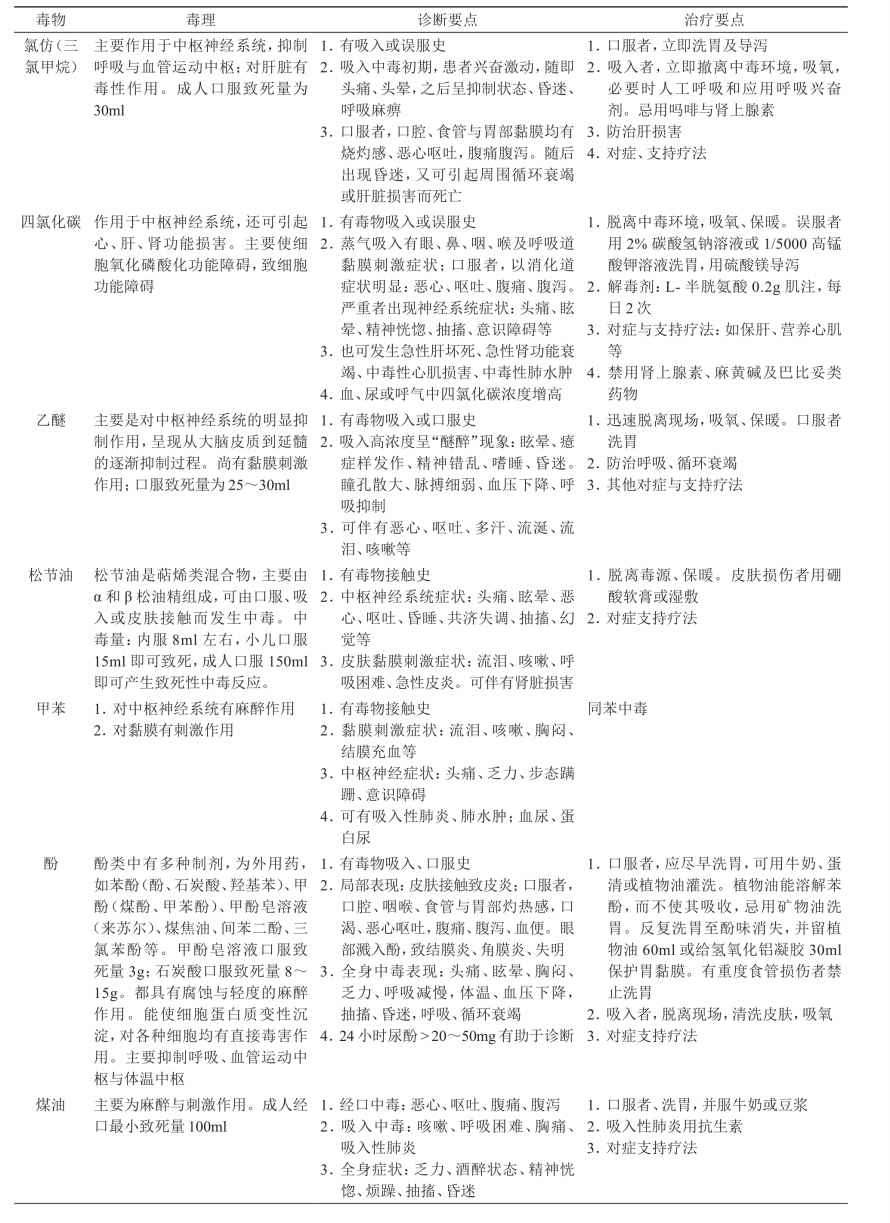
\includegraphics[width=\textwidth,height=\textheight,keepaspectratio]{./images/Image00217.jpg}\\
 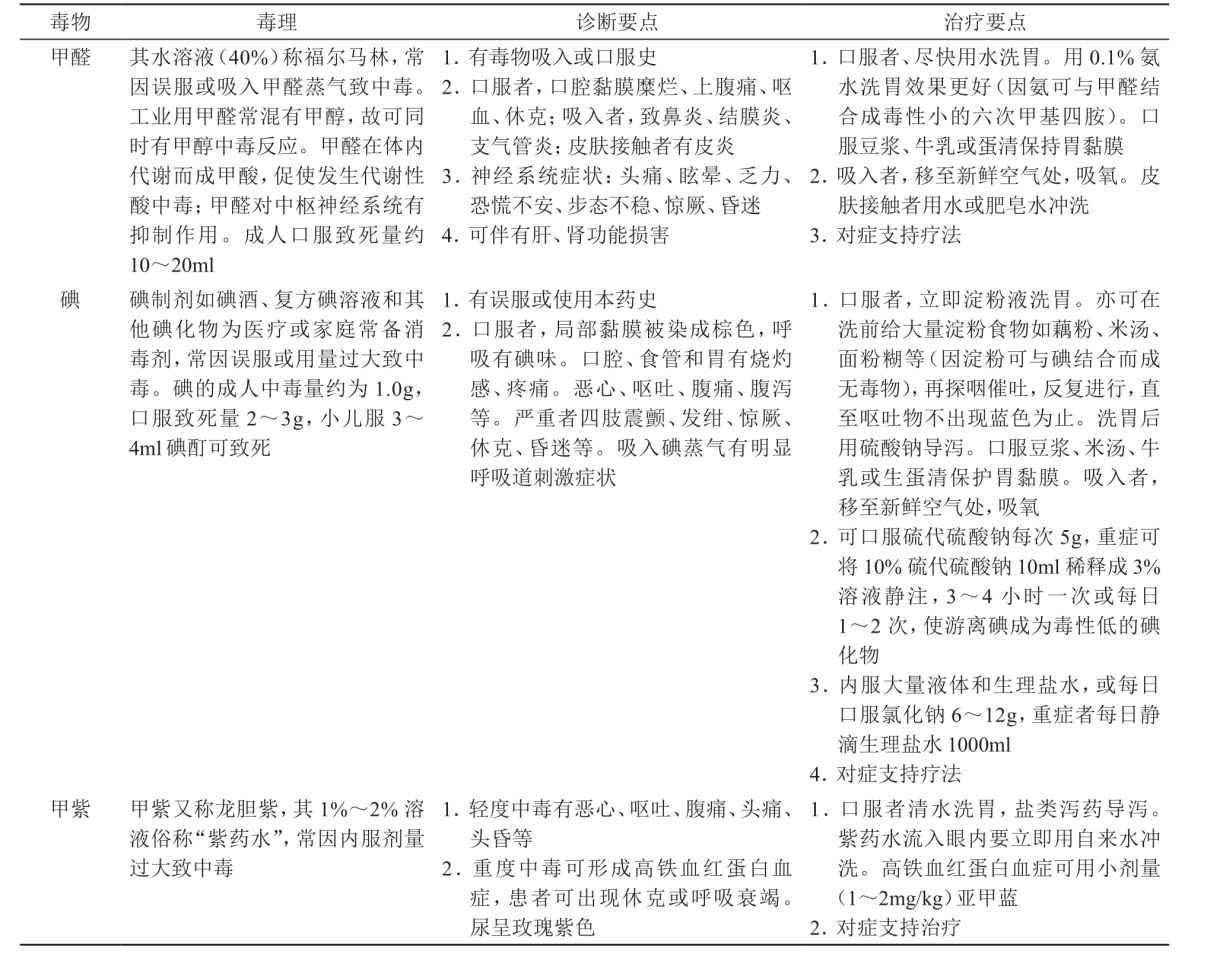
\includegraphics[width=\textwidth,height=\textheight,keepaspectratio]{./images/Image00218.jpg}
 \end{longtable}

\protect\hypertarget{text00156.html}{}{}

\hypertarget{text00156.htmlux5cux23CHP5-5-6}{}
参 考 文 献

1. 陈灏珠 ,林果为.实用内科学.第13版.北京:人民卫生出版社,2009

2. 任引津
,张寿林,倪为民,等.实用急性中毒全书.北京:人民卫生出版社,2003

3. 朱子扬
,龚兆庆,汪国良.中毒急救手册.第3版.上海:上海科学技术出版社,2007

4. 陆再英 ,钟南山.内科学.第7版.北京:人民卫生出版社,2008

\protect\hypertarget{text00157.html}{}{}

\chapter{金 属 中 毒}

\section{铅中毒}

铅是一种柔软成蓝灰色的金属,可溶于酸。铅及其化合物在生产、生活中应用广泛,常见铅化合物有:一氧化铅(有黄丹和密陀僧两种)、二氧化铅(过氧化铅)、四氧化铅(铅丹、红丹、广丹、樟丹)、氯化铅、硫酸铅、硝酸铅、醋酸铅(铅糖)、硅酸铅及碳酸铅(铅白)等,对人均有较大毒性。铅能干扰卟啉代谢,引起溶血及血管痉挛,临床上主要表现为腹绞痛以及神经系统、肝脏、肾脏和血液系统异常。

\subsection{病因与发病机制}

铅吸收后进入血液循环,主要以磷酸氢铅(PbHPO\textsubscript{4}
)、甘油磷酸化合物、蛋白复合物或铅离子状态分布全身各组织脏器,主要分布在细胞核和胞浆的可溶性部分以及线粒体、溶酶体、微粒体中。最后约有95\%的铅以不溶性的正磷酸铅{[}Pb\textsubscript{3}
(PO\textsubscript{4} )\textsubscript{2}
{]}稳定地沉积于骨骼系统,其中以长骨小粱为最多。仅5\%左右的铅存留于肝、肾、脑、心、脾、基底核、皮质灰白质等器官和血液中。血液中的铅约95\%分布在红细胞内,主要存在于红细胞膜内。骨铅与血铅之间处于一种动态平衡,当血铅达到一定程度时,就可引起急性中毒症状。吸收的铅主要通过肾脏排出,部分经粪便、乳汁、胆汁、月经、汗液、唾液、头发、指甲等排出。沉积在骨骼中的铅的半衰期约20余年。铅对神经、血液、消化、血管系统和肾脏均有毒性。人口服铅的最小致死量为5mg/kg。

铅中毒的机制主要有:①对血液系统的影响:铅引起血红蛋白合成障碍。首先抑制δ-氨基-乙酰酮戊酸(ALA)合成酶和ALA脱水酶,使卟胆原合成受阻;铅又抑制血红蛋白合成酶,阻碍原卟啉与二价铁结合为正铁血红素。引起原卟啉、ALA和粪卟啉在血液中积累,后两者随尿排泄。红细胞内原卟啉部分与锌离子络合成锌原卟啉(ZPP),其余以游离原卟啉(FEP)存在于红细胞内。因而铅接触者的血中ZPP和FEP两者均可增高。由于铅对幼红细胞嘧啶-5'{-}核苷酸酶有抑制作用,使大量嘧啶核苷酸蓄积在细胞质内,阻碍微粒体RNA的降解,而导致嗜碱性点彩细胞的增多。铅阻碍原卟啉与铁结合,铁以铁蛋白形式沉积在骨髓幼红细胞内,可形成环形铁粒幼细胞。高浓度铅对成熟红细胞膜有直接损伤作用,引起溶血。②血管痉挛;铅引起卟啉代谢障碍,抑制细胞含巯基的酶,干扰自主神经,或直接作用于平滑肌,故可导致血管痉挛,从而引起内脏缺血。临床上铅中毒时,铅容、腹绞痛、中毒性脑病等均可能与血管痉挛有关。③干扰脑的代谢:铅对中枢神经系统的损害,认为是阻碍γ-氨基丁酸(GABA)功能,降低细胞色素C浓度,加速多巴胺释放,减少细胞外钙离子浓度,影响乙酰胆碱(ACh)释放等,最终引起各种行为和神经效应的改变。严重中毒可致神经细胞退行性改变。铅可引起周围神经Schwann细胞肿胀、节段性脱髓鞘和轴索改变,导致周围神经麻痹。铅尚能使肌肉内磷酸肌酸再合成受阻,引起瘫痪。通过与钙直接竞争,干扰钙进入细胞以及细胞内贮钙池的动员等过程而影响钙稳态,干扰钙对神经递质的释放,影响神经系统的生理功能。④四乙铅为剧毒的神经毒物,在肝脏的微粒体中迅速转化为毒性更大的三乙铅,主要抑制脑的葡萄糖氧化和单胺氧化酶,前者减少高能磷酸键的形成,引起细胞呼吸障碍,导致细胞缺氧;后者使5-羟色胺在大脑积聚。四乙铅还抑制胆碱酯酶活力,影响肾上腺素能和胆碱能神经纤维。轻者使大脑皮质功能失调和自主神经功能紊乱,严重时损害神经细胞,出现脑水肿和弥散性脑损伤。⑤肾脏损害:铅可损害肾小管上皮细胞线粒体的功能,抑制ATP酶而干扰主动转运机制,损害近曲小管重吸收功能,继而GFR降低,尚可引起间质性肾炎。引起肾近曲小管损伤的血铅阀值为2.88μmol/L。⑥对生殖系统及子代的影响:铅具有生殖毒性、胚胎毒性和致畸作用。铅对人类生殖功能影响与剂量有关,近来报道血铅在25~40μg/dl就可影响男性生殖功能,使精子畸形。孕妇体内的铅可以顺利通过胎盘,作用于胚胎。孕妇头3个月如处于较大剂量的铅暴露中可以引起死胎、流产、胎儿畸形,并可影响子代身体发育和智商发育等。

\subsection{诊断}

铅中毒的诊断要点是:①有铅及其化合物接触史;②有典型的临床症状和体征;③尿铅或血铅浓度明显升高。

\paragraph{铅接触史}

急性铅中毒大多系口服可溶性铅无机化合物和含铅药物如黑锡丹、樟丹(系用于治疗癫痫和哮喘的偏方)等引起。慢性铅中毒多见于长期吸入铅烟、铅尘的工人,发病率以铅冶炼和蓄电池制造行业较高,铸字、颜料、釉彩、焊接少见。长期应用含铅的食具如锡器盘、铅壶、彩釉陶器、铅绘粉涂里的玻璃杯等盛饮料或食品,可引起慢性中毒。四乙铅是铅的有机化合物,是一种无色油状液体,挥发性强,主要用作汽油抗爆剂,可经呼吸道、皮肤、消化道吸收而中毒。

\paragraph{临床表现特点}

\hypertarget{text00157.htmlux5cux23CHP5-6-1-2-2-1}{}
(1) 急性中毒:

急性铅中毒多因误服经消化道吸收引起。患者服含铅化合物4~6小时后,个别长至1周出现恶心、呕吐,呕吐物为白色奶块状(含氯化铅),口内有金属味,腹绞痛,腹泻,解黑便(含硫化铅),血压升高,少数患者发生消化道出血和麻痹性肠梗阻。严重中毒数日后出现贫血(伴有嗜碱性点彩红细胞和网织红细胞明显增多)、中毒性肾炎、中毒性肝炎和多发性周围神经病变和铅毒性脑病(抽搐、谵妄、高热、昏迷等)。其中,腹绞痛是急性中毒的早期突出症状,也可能是慢性铅中毒急性发作的症状,诱因常是饮酒、感染、吃酸碱食物等;腹绞痛发作突然、剧烈难忍、部位不定、阵阵发作,每次持续数分钟到数小时;发作时面色苍白、焦虑不安、出冷汗,呈蜷曲体位。

\hypertarget{text00157.htmlux5cux23CHP5-6-1-2-2-2}{}
(2) 急性四乙铅中毒:

由短期内大量吸入或皮肤吸收所致,潜伏期一般为6小时~11天(吸入高浓度者可立即昏迷)。轻者有头痛、头晕、噩梦、乏力、纳差、恶心、呕吐、关节疼痛;较重者出现自主神经系统症状,如多汗、唾液分泌增多、血压下降、脉率缓慢,严重者有幻觉、妄想、烦躁、谵妄、全身抽搐甚至瞳孔散大、意识丧失。血压降低、脉率低、体温低为四乙铅中毒体检的“三低征”。发作可呈间歇性,间歇期间患者常表情痴呆、动作迟缓,说话含糊或呈木僵状态。

\hypertarget{text00157.htmlux5cux23CHP5-6-1-2-2-3}{}
(3) 慢性铅中毒:

职业性铅中毒以慢性中毒居多。非职业性慢性中毒可因长期用含铅锡壶饮酒,服用含铅中成药以及环境污染所致。典型表现有:①腹绞痛。②周围神经炎:表现为运动和感觉障碍,重症患者可发生垂腕、垂足,谓之铅中毒麻痹。③中毒性脑病:常有神经衰弱症状,几周或几个月后出现躁狂、谵妄、视力减退以至失明、失语、麻痹、幻觉、妄想、头痛、呕吐、昏迷等症状。④明显贫血。但近年来上述典型表现已罕见。多见的为轻度中毒患者,症状有头晕、乏力、食欲不振、腹胀、脐周隐痛、便秘和肌肉关节酸痛等非特异性症状。口中金属味和齿龈铅线已很少发现。有些患者可无明显症状,而仅有周围神经的感觉和运动神经传导速度减慢及尿中出现低分子量的β2-微球蛋白。⑤中毒性肾病:对肾脏的损害早期主要在肾小管:尿中出现低分子量β2-微球蛋白、糖尿,NAG活性增高;尿6-酮前列腺素F1α(6-Keto-PGF1α)排出减少和血栓素B\textsubscript{2}
(TXB\textsubscript{2}
)排出增加。早期肾脏损害经驱铅治疗可恢复,后期则可发生肾小管萎缩、间质纤维化,甚至肾小球硬化,可导致肾功能不全。妇女可不育、流产、早产、死胎。男性精液中精子减少,活动减弱和形态改变。

\paragraph{辅助检查}

①血铅:铅中毒时,血铅浓度的增高出现较早,含量较稳定,不受肾功能影响。正常值上限为2.4μmol/L(50μg/L)。但血铅仅反应体内有害作用的铅量,不能完全代表体内铅总量水平。②尿铅:在一般铅接触的情况下,尿铅可反映血铅的浓度,也可反映体内总铅量。但易为环境因素污染,并受尿量和肾功能影响,因而波动较大。正常值上限0.39μmol/L(0.08mg/L)。③驱铅试验:可反映体内铅负荷。对怀疑为铅中毒,但尿铅测定正常者,可进行此试验。方法是:依地酸钙钠(EDTA
Ca-Na\textsubscript{2} ) 1g加入 5\%葡萄糖溶液
250~500ml中,静滴4小时,用药开始时即留24小时尿。不接触铅的正常人尿铅不超过0.3mg/24h,铅接触者尿铅超过1mg/24h,提示为中毒的高危者。④ZPP(正常值上限0.9~1.79μmol/L)和FEP(正常值上限0.72~1.78μmol/L)增高和血ALA脱水酶(正常值217.6
±
46.6U)降低,尿ALA(正常值上限30.5μmol/L)增高和粪卟啉(正常值:定量0.15mg/L,定性+)异常。脱离铅接触后ALA脱水酶、ALA和尿粪卟啉在数日后即可转为正常,而ZPP和EPP仍可持续增高2~3个月之久。故目前认为ZPP和FEP是铅接触较持久的灵敏指标。中毒后血中点彩红细胞(正常值:300个/100万红细胞)增高,但由于其计数繁复,目前多已不采用。铅毒性贫血多属轻度,可呈低色素性。⑤铅中毒患儿的粪便偶见鲜血或潜血,由于大量铅质刺激肠道所致。此外,血糖往往增加。

\paragraph{鉴别诊断}

急性铅中毒要与急性肠胃炎、出血性肠炎、急腹症等鉴别。慢性铅中毒诊断较困难,其周围神经炎和肾功能损害要除外药物副作用、糖尿病等代谢性疾病和其他血管病变。

\subsection{治疗}

\paragraph{一般处理}

皮肤污染宜彻底清洗;吸入中毒者宜迅速脱离有毒环境;口服中毒者应立即洗胃和导泻。洗胃可用1\%硫酸钠或硫酸镁,以形成不溶性硫酸铅而免于吸收,口服硫酸镁(钠)20g导泻。亦可口服活性炭20g以吸附胃内容物。

\paragraph{驱铅治疗}

驱铅治疗是治疗铅中毒成功的关键。常用药物有:①依地酸钙钠(EDTA
Ca-Na\textsubscript{2}
):每日1.0g加入5\%葡萄糖溶液250ml中静滴;或0.25~0.5g,每日2次,肌肉注射。连续3天为1疗程,停药4天后再给1疗程,一般用药2~4个疗程。本药为目前驱铅治疗的首选药物,可以迅速改善症状,使尿ALA、粪卟啉在短期内下降。②二乙烯三胺五乙酸三钠钙(促排灵,Na\textsubscript{3}
Ca-EDTA):驱铅作用比依地酸钙钠强。剂量0.5~1.0g/d溶入生理盐水250ml静滴或配成10\%~25\%溶液肌注,疗程同依地酸钙钠。③巯基络合剂:二巯丁二钠(Na-DMS)每次1g缓慢静脉注射;或二巯丁二酸(DMSA)0.5g,每日3次口服;两药疗程与Na\textsubscript{2}
Ca-EDTA相同。DMSA性质稳定,应用方便,副作用小、安全,已在全国推广使用。④巯乙胺:用于急性四乙铅中毒,能减轻神经症状。剂量为200~400mg加入5\%葡萄糖溶液中静滴。肝、肾功能损害者禁用。

铅中毒性脑病宜用二巯丙醇(BAL)和EDTA联合疗法。剂量BAL
4mg/kg,每4~6小时一次,肌肉注射;EDTA Ca-Na\textsubscript{2}
12.5mg/kg,每日2次,加入5\%葡萄糖溶液中滴注或肌肉注射。两药同时用3~5天。严重者用皮质激素,颅内压增高者用脱水剂。

\paragraph{对症处理}

腹绞痛用阿托品0.5mg肌肉注射或10\%葡萄糖酸钙10ml静脉注射。钙剂可将血中铅迅速转移至骨内,解除急性中毒症状。可用10\%葡萄糖酸钙10ml静注,每日2~3次;或口服乳酸钙或其他钙剂,每日2g,1天3次,待急性期过后,再做驱铅治疗。若中毒症状不严重,驱铅则应是首要任务,则宜单独驱铅治疗。原因是不用钙剂,可避免第二次驱铅治疗时,使沉积于骨骼中的铅再度入血,引发高铅血症的腹痛等症状。

\hypertarget{text00157.htmlux5cux23CHP5-6-1-4}{}
参 考 文 献

1. 王汉斌,牛文凯.金属和类金属中毒诊治概述.中国医刊,

2008,43(10):6

2. 张文武.急诊内科学.第2版.北京:人民卫生出版社,2007

3. 陈灏珠 ,林果为.实用内科学.第13版.北京:人民卫生出版社,2009

4. 任引津
,张寿林,倪为民,等.实用急性中毒全书.北京:人民卫生出版社,2003

\protect\hypertarget{text00158.html}{}{}

\section{汞中毒}

金属汞(mercury)又名水银,常温下为液态的银白色金属,具有易蒸发的特性。常见的汞化合物有硫化汞、氯化汞、氯化亚汞和氧化汞。通常称为轻粉(又称水银粉、汞粉、甘汞)的化合物,主要含氯化亚汞;白降丹(又称降丹、水火丹、升汞)主要含氯化汞(氯化高汞)和氯化亚汞;红升丹(又称升药、红粉、小金丹)主要含氧化汞。中药朱砂主要成分为硫化汞。汞及其化合物可通过呼吸道或皮肤吸收而中毒,但以呼吸道吸入中毒最常见,偶尔有误服而中毒者,皮肤接触中毒者罕见。有机汞农药目前在国内已停产,故急性有机汞中毒已基本绝迹。误服金属汞后迅速从胃肠道排出,吸收甚微,一般不引起中毒。

\subsection{病因与发病机制}

汞蒸气由呼吸道吸收,金属汞由消化道吸收甚微(约为摄食量的万分之一),但氯化汞(HgCl\textsubscript{2}
)则吸收迅速。汞盐也可由皮肤黏膜吸收。金属汞和一价汞化合物进入血液后,在血内可氧化为二价汞离子,后者与血浆蛋白、血红蛋白结合,形成蛋白结合型汞。汞还可以与体液中阴离子结合,也可以与含巯基的低分子化合物如半胱氨酸、还原型谷胱甘肽结合,形成可扩散型汞。这两型汞随血液分布到各组织器官,其中以肾含量最高。汞蒸气吸入后,可透过血脑屏障进入脑内,主要蓄积于脑干和小脑。汞主要由尿和粪中排出,唾液、乳汁、汗液亦有少量排泄,肺部呼出甚微。汞是许多酶的非特异性抑制剂。汞离子对巯基、二巯基具有高度亲和力,使体内具有重要生物活性的巯基有关的酶,如细胞色素氧化酶、丙酮酸激酶、琥珀酸脱氢酶等失去活性;汞还与氨基、羧基、磷酰基结合而影响功能基团的活性。由于这些酶和功能基团的活性受影响,阻碍了细胞生物活性和正常代谢,最终导致细胞变性和坏死,从而引起中枢和自主神经系统功能紊乱和肾、消化道等脏器损害。汞离子还可导致细胞外液的钙离子大量进入细胞内,引起“钙超载”,造成组织细胞严重缺血缺氧。汞还可引起免疫功能紊乱,产生自身抗体,发生肾病综合征或肾小球肾炎。汞由唾液排出与口腔内食物残渣分解产生的硫化氢相结合生成硫化汞,对口腔黏膜有强烈的刺激作用。人吸入1~3mg/m\textsuperscript{3}
的汞蒸气数小时即可发生急性中毒。

升汞致死量为0.3~0.5g,氧化汞为1~1.5g,甘汞为2~3g。

\subsection{诊断}

\subsubsection{毒物接触史}

职业性急性中毒因意外事故、土法炼金、镏金、首饰加工等,多为个体生产,设备简陋,通风不良所致,均经呼吸道吸入。非职业性大多数是使用含汞中药偏方如轻粉(氯化亚汞)治病(如银屑病、湿疹、皮炎、哮喘等),也有误服(升汞、甘汞)、自杀和他杀者。通过吸入其蒸气、口服或涂敷皮肤处而引起中毒。也有经静脉、皮下注入汞而中毒者。

\subsubsection{临床表现特点}

\paragraph{急性汞中毒}

主要由口服升汞等汞化合物引起。患者在服后数分钟到数十分钟即引起急性腐蚀性口腔炎和胃肠炎。患者诉口腔和咽喉灼痛,并有恶心、呕吐、腹痛,继有腹泻。呕吐物和粪便常有血性黏液和脱落的坏死组织。口腔可见牙龈红肿、糜烂、出血,口腔黏膜溃疡,牙龈松动、流涎,口内腥臭味。患者常可伴有周围循环衰竭和胃肠道穿孔。在3~4天后(严重的可在24小时内)可发生急性肾功能衰竭,同时可有肝脏损害。

吸入高浓度汞蒸气中毒潜伏期数小时、数日或数周不等,可引起咳嗽、咽痛、发热、咯血丝痰等刺激症状,严重者可并发间质性肺炎、急性肺水肿、呼吸衰竭。神经系统可出现头昏、头痛、倦怠、手抖、嗜睡或兴奋、衰弱等,个别严重病例可陷入昏迷,最后因休克而死亡。亦可发生中毒性肝病、急性肾功能衰竭。

皮肤接触汞及其化合物可引起接触性皮炎,具有变态反应性质。皮疹为红斑丘疹,可融合成片或形成水疱,严重者发生剥脱性皮炎,愈后遗有色素沉着。

\paragraph{慢性汞中毒}

常为职业性吸入汞蒸气所致,少数患者亦可由于应用汞制剂引起。目前由于使用美白化妆品致汞中毒者日渐增多。精神-神经症状可先有头昏、头痛、失眠、多梦,随后有情绪激动或抑郁、焦虑和胆怯以及自主神经功能紊乱的表现如脸红、多汗、皮肤划痕征等。肌肉震颤先见于手指、眼睑和舌,以后累及手臂、下肢和头部,甚至全身;在被人注意和激动时更为明显。口腔症状主要表现为黏膜充血、溃疡、齿龈肿胀和出血,牙齿松动和脱落。口腔卫生欠佳者齿龈可见蓝黑色的硫化汞细小颗粒排列成行的汞线,是汞吸收的一种标记。肾脏方面,初为亚临床的肾小管功能损害,出现低分子蛋白尿等,亦可出现肾炎和肾病综合征。肾脏损害在脱离汞接触后可望恢复。慢性中毒患者尚可有体重减轻、性功能减退,妇女月经失调或流产以及有甲状腺功能亢进、周围神经病变。眼晶状体前房的棕色光反射,认为是汞沉着引起的“汞晶状体炎”,在中毒症状消失或脱离汞接触后,这种棕色光反射仍可持久存在,是一种汞吸收的另一标记。

\paragraph{汞中毒临床分型}

①观察对象:患者有神经衰弱症状群,或呼吸道刺激症状,而无任何脏器损害的病征者。脱离接触后健康恢复。②轻度中毒:表现为腹痛、腹泻、发热、汞毒性口炎,尿汞值明显超标。③中度中毒:除上述症状外,表现为肢体感觉、运动障碍及肾功能损害病征者。④重度中毒:表现为中毒性肺炎、肺水肿、肝功能衰竭、肾功能衰竭、中枢性高热、休克或其他严重并发症者。

\subsubsection{辅助检查}

\paragraph{尿汞测定}

在一定程度上反映体内汞的吸收量,但常与汞中毒的临床症状和严重程度无平行关系。尿汞正常值因化验方法和所在地区而异,国内尿汞正常上限值一般不超过250nmol/L(0.05mg/L)(二硫腙热硝化法)、0.01mg/L(蛋白沉淀法)、0.02mg/L(原子能吸收法)。

\paragraph{血汞 、发汞测定}

血汞正常上限值为0.15μmol/L
(0.03mg/dl),发汞不超过4mg/100g,唾液汞约为尿汞的10\%。血汞、发汞和唾液汞含量增高均亦提示体内过量汞吸收,但与中毒症状不一定相关。

\paragraph{驱汞试验}

可用二巯丙磺钠0.25g,肌肉注射,或二巯丁二钠0.5g静脉注射,如尿汞排出量明显增高,提示体内汞负荷过量。可作为重要的辅助诊断依据。

\paragraph{其他}

慢性汞中毒患者可有脑电图波幅和节律电活动改变,周围神经传导速度减慢,血中α\textsubscript{2}
球蛋白和还原型谷胱甘肽增高,以及血中溶酶体酶、红细胞胆碱酯酶和血清巯基等降低。

\subsubsection{诊断注意事项}

急性汞中毒的诊断主要根据职业史或摄入毒物史,结合临床表现和尿汞或血汞测定(明显增高)而确立。慢性汞中毒的诊断,应强调接触史,临床有精神-神经症状、口腔炎和震颤等主要表现,并需除外其他病因引起的类似临床表现。尿汞和血汞等测定值增高对诊断有辅助意义。驱汞试验如尿汞排出量明显增高,可作为重要的辅助诊断依据。

\subsection{治疗}

\subsubsection{清除毒物}

吸入中毒者立即搬离中毒环境,除去污染的衣服,卧床休息,保温,呼吸频速者给予吸氧,以及相应的对症治疗。口服中毒者及早洗胃,先口服或从胃管注入活性炭15~20g混悬液,以吸附胃内的汞,随后可选用2\%碳酸氢钠溶液、温水洗出,并继续彻底洗胃(注意:忌用生理盐水洗胃,尤其是升汞中毒时,因能增加其溶解度,增加吸收)。导泻用50\%硫酸镁40ml口服或胃管灌入,如腹泻已很重,则不必导泻。但是,若服毒时间较长,或消化道症状剧烈,或呕吐物有咖啡色胃内容物或血性呕吐物,则洗胃取慎重态度,以免招致胃穿孔。此时宜以多次口服牛奶、鸡蛋清,每次300~500ml,蛋白质既能保护胃黏膜,又能与汞结合而阻止汞的吸收。对口服升汞的中毒者,可及早给予口服Carter解毒液(磷酸钠1~2g、醋酸1g,溶于200ml温开水中配成),分4~6次口服,每小时1次,但本法对毒物已吸收者无效。

\subsubsection{驱汞治疗}

应尽早应用解毒剂,最好在出现肾功能损害前用药。制定驱汞治疗方案时,驱汞药物剂量大小、用药次数和疗程长短应依据病情严重程度而异。总的原则是既达到驱汞目的,也应尽量降低络合综合征的发生。常用药物如下:

\paragraph{二巯丙磺钠(unithiol,二巯基丙磺酸钠)}

其巯基可与汞离子结合成巯-汞复合物,随尿排出,使组织中被汞离子抑制的酶得到复能。急性中毒时的首次剂量为5\%溶液2~3ml,肌肉注射;以后每4~6小时一次,每次1~2.5ml。
1~2天后,每日一次,每次2.5ml。一般治疗1周左右。必要时可在1个月后再行驱汞。由于连续给药7天,在头5天内排出的尿汞量可占体内整个积储量的97\%,故是否给予第二疗程,取决于尿汞测定结果。常见副作用有头晕、头痛、恶心、食欲减退、无力等,偶尔出现腹痛或低血钾,少数患者出现皮疹,个别发生全身过敏性反应或剥脱性皮炎。如有肾功能损害,上述药物慎用。

\paragraph{二巯丙醇}

其药理作用与二巯丙磺钠相似。首次剂量为2.5~3.0mg/kg体重,每4~6小时深部肌肉注射1次,共1~2天。第3天按病情改为每6~12小时1次;以后每日1~2次。共用药10~14天。常见副作用有头痛、恶心、咽喉烧灼感、流泪、鼻塞、出汗、腹痛、肌肉痉挛、心动过速、血压升高、皮疹和肾功能损害等。小儿易发生过敏反应和发热。

\paragraph{二巯丁二钠}

首剂2g,溶入生理盐水20~40ml中静脉注射;以后每日1g,共4~5天。

\paragraph{乙酰消旋青霉胺}

以上药物无效时可考虑用本药。青霉胺有右旋、消旋、乙酰消旋三种化合物,解毒效果以乙酰消旋青霉胺为最好。用法:每日1g,分4次口服,同时加服维生素B\textsubscript{6}
100mg/d。副作用有乏力、头晕、恶心、腹泻、尿道排尿灼痛。少数出现发热、皮疹、淋巴结肿大等过敏反应和粒细胞减少。青霉素过敏者不用。

慢性汞中毒的驱汞治疗:5\%二巯丙磺钠2.5~5.0ml肌肉注射,每日1次,连续3天,停药4天为1疗程。一般用药2~3疗程。此外,二巯丁二酸钠和青霉胺亦为常用驱汞药物。硫胺-8-6-乙酰双氢硫辛酸甲酯硫化物,每日口服400mg,可使尿汞排泄量增加2~6倍。间-二巯基琥珀酸0.5g,每日3次,连服5天,可使尿汞排泄比治疗前增加8倍。

\subsubsection{细胞活性药物的应用}

复方丹参注射液、大剂量维生素C、细胞色素C、ATP、辅酶A、葡萄糖醛酸内酯等,分别加入葡萄糖溶液中静滴,每日1~2次。维生素B\textsubscript{1}
、维生素B\textsubscript{6}
等,每日1次,肌肉注射。借以保护神经、心、肾、肝等功能。

\subsubsection{对症处理}

在急性中毒治疗过程中应注意水、电解质和酸碱平衡并纠正休克。出现有肾功能损害和急性肾功能衰竭时应避免应用驱汞药物,并应及早进行血液透析或血液灌洗,此时可同时应用驱汞药物,以减少汞对人体的毒性。防治络合综合征,补充铜、铁、锌等必需微量元素。有神经衰弱或轻度兴奋症状表现的,可应用吡拉西坦(脑复康)、复方吡拉西坦脑蛋白水解物片(康脑灵)、还原型谷胱甘肽钠(谷拉定)等。口腔病变可用3\%过氧化氢溶液漱口或0.1\%~0.2\%乳酸依沙吖啶溶液(利凡诺溶液)含漱,并涂以4\%鞣酸甘油。皮肤发疹渗出糜烂者可用3\%~5\%硫代硫酸钠溶液湿敷或涂抹2\%~3\%二巯丙醇软膏。酌情使用解痉止痛药、镇静药。应用抗生素防治皮肤、肺部等感染。

\subsection{预防}

对于工业上常接触汞的人来说,要注意以下几点:用无毒或低毒物质代替汞;加强通风排毒设施;防止汞的二次污染,如建造物表面涂氯乙烯漆,减少汞蒸气渗透和吸附;加强个人防护。

对普通百姓来说,要注意:服用中药,选用美白化妆品要谨慎,就诊正规医院看病,购买化妆品时要看清有无化妆品批准文号;购买荧光灯时,买弯不买直,买细不买粗,不要摔破废弃的荧光灯管;补牙时尽量避免使用银汞合金材料。

\hypertarget{text00158.htmlux5cux23CHP5-6-2-5}{}
参 考 文 献

1. 杨水莲
,李晓军,冯克玉,等.我国汞中毒临床研究概况.中国职业医学,2004,31(6):50-52

2. Jon KC,Yoong MRCP. Heavy-Meals of Mercury. N Engl J
Med,2006,354:e3

3.
王广松,王明启.汞职业危害防治研究中使用汞中毒诊断标准(GBZ89-2002)的体会.职业卫生与病伤,2004,19
(3):179-180

4.
李树强,赵金垣,徐希娴.不同接触途径所致急性亚急性汞中毒的分析研究.中国工业医学杂志,2003,16(6):324-327

5. 李艳艳
,熊光仲.汞中毒的毒性机制及临床研究进展.中国急救复苏与灾害医学杂志,2008,1(18):57-59

6. Carvalho CM,Chew EH,Hashemy SI,et al. Inhibition of the human
thioredoxin system. The journal of Biological
Chemistry,2008,18(283):11913-11923

7. 杨萍
,王瑾.化妆品中汞含量及化妆品致汞中毒概况.职业与健康,2010,17(26):2010-2011

\protect\hypertarget{text00159.html}{}{}

\section{铊中毒}

铊(Thallium,Tl)是一种稍带蓝色的银白色稀有金属,呈四角形结晶,金属铊单体基本无毒,溶于酸后形成的铊化合物无色无味,毒性剧烈。常见铊化合物有醋酸铊、硫酸铊、溴化铊与碘化铊,铊化合物有一价和三价两种,后者不稳定,毒性小于一价铊盐,遇碱或水解为一价化合物。铊化合物曾经作为杀鼠剂和治疗多汗症的药物广泛使用,但不久即发现其毒副作用剧烈而停止使用。在铊提取和化合物生产过程中,可能发生职业性或环境性铊中毒。近年来,由于铊中毒的隐匿性,铊盐投毒案件时有发生,且由过去环境污染或职业接触的中毒方式转向为人为投毒,严重地威胁着人民群众的身体健康。

\subsection{病因与发病机制}

铊及铊化合物可以经由呼吸系统、消化系统、皮肤等途径快速进入体内,但主要是经消化道进入,其次是呼吸道,可溶性的铊被胃肠道吸收后,不与血清蛋白结合,而以离子形式进入血液,存在于红细胞中并随血液到达全身的器官和组织,有报道铊中毒患者血细胞铊含量较血浆高9倍。组织对铊的吸收类似于钾离子,肾脏中铊含量最高,其次是睾丸,其他依次为肌肉、淋巴结、胃肠、心脏、脾脏、肝脏,皮肤和毛发中含一定量铊。铊能通过血脑屏障,进入速度比进入其他器官慢,同样脑中铊的清除速度也比在其他器官慢,灰质中铊浓度是白质的3倍。铊主要通过肾脏和肠道排出,少数可通过乳汁、汗腺、泪液、毛发和唾液排出。

铊和铊化物在体内的中毒机制目前尚未完全清楚。主要有以下几种观点:①许多研究表明,铊和铊化物进入体内后,可溶性的铊离子与体内的生物分子(如酶类)中的基团---SH、---NH\textsubscript{2}
、---COOH、---OH等结合,导致其生物活性丧失,如铊与蛋白和酶分子上的巯基结合可干扰其生物活性,使动物血清中巯基含量下降;与半胱氨酸巯基结合影响毛囊角蛋白的合成导致脱发;引起肝内还原型谷胱甘肽减少导致过氧化损伤,引起肝、肾损害;铊与线粒体氧化呼吸链中含巯基的酶结合,可导致氧化-磷酸化脱耦联,干扰能量的产生,神经系统则首先受到影响,从而使组织功能出现障碍。②铊离子对钾离子有拮抗抑制作用,铊与钾理化性质相近,进入细胞内不易排出,铊与钠-钾ATP酶的亲和力比钾大10倍,当铊在细胞内聚积,可替代钾参与酶学反应,在较低浓度时起兴奋作用,在高浓度时就起抑制作用。通过竞争抑制钾离子的生理作用,可影响能量生成,产生铊中毒效应,干扰一些依赖钾的关键生理过程。③铊离子可与核黄素(维生素B\textsubscript{2}
)结合,使细胞能量代谢发生改变,敏感的神经细胞容易受到损伤。铊还可以通过血脑屏障,在脑内蓄积,而产生明显的神经毒作用,同时铊离子可以通过胎盘屏障,给胎儿期发育迅速的神经系统造成伤害。④铊具有明显的细胞毒性,这种毒性抑制细胞的有丝分裂,造成细胞代谢紊乱,干扰DNA的合成,诱发染色体突变,是一种致突变物。

铊化合物对人的急性毒性剂量为6~40mg/kg体重,儿童相对更为敏感,为8.8~15mg/kg体重,成人最小致死量(MLD)为12mg/kg体重。

\subsection{诊断}

\subsubsection{毒物接触史}

职业性急性中毒因意外事故、矿石加工、工业生产等,以胃肠道摄入、皮肤接触为主,少数经呼吸道摄入。非职业性大多数是使用不明来源的中药偏方治病(如多汗症、毛发脱落),也有误服铊盐溶液及自杀者,极少数投毒事件当中中毒者被人经静脉注射中毒。

\subsubsection{临床表现特点}

\paragraph{急性铊中毒}

以胃肠道摄入起病多见,急性铊中毒一般于接触后12~24小时发病。早期表现主要为恶心、呕吐、腹部绞痛或隐痛、腹泻等;严重者可出现消化道出血,并于2~5天后出现对称性指(趾)端酸、麻、疼痛,逐渐加剧并向近心端进展,轻触皮肤即疼痛难忍,以致不能站立与行走。如未及时诊治,病情可发展为肢体瘫痪、肌肉萎缩。铊中毒时脑神经常受累,如视力减退、眼肌麻痹、周围性面瘫等。当中枢神经系统受损时,轻者有头痛、睡眠障碍、情绪不稳等表现;重者出现嗜睡、谵语、精精失常、抽搐甚至昏迷,部分中毒量大者可因呼吸循环功能衰竭而死亡。

脱发是铊中毒的特异性表现,常于急性中毒后1~3周出现,头发呈簇状脱落,表现为斑秃或全秃,严重者在10~20天内出现胡须、腋毛、阴毛和眉毛全部脱落,一般在毛发脱落后第四周开始再生,约三个月后完全恢复。此外,皮肤干燥、脱屑,出现皮疹、痤疮、皮肤色素沉着、手掌及足跖部角化过度,指甲和趾甲于第4周可出现白色横纹,称为“米氏纹”。部分患者有肝、肾、心肌损害的临床表现。因此,人们将胃肠炎、多发性神经病和脱发三联症看作是铊中毒的典型症状。

\paragraph{慢性铊中毒}

由长期职业性接触铊及铊化合物导致,慢性铊中毒与急性铊中毒的症状基本相同,只是临床表现较为轻缓。非职业性慢性中毒大多是因为食用了生长在被铊污染过的土壤里的蔬菜水果或粮食等作物,或许是因饮用了被铊污染的水所致。慢性铊中毒常出现乏力、四肢发麻等症状,肌电图显示对称性周围神经损害;同样,在中毒后4周左右指甲和趾甲可出现白色横纹(米氏纹)。持续接触含铊化合物还可引起视网膜炎、球后视神经炎及视神经萎缩等。

\subsubsection{辅助检查}

\paragraph{血铊 、尿铊测定}

现多采用石墨炉原子吸收法(GFAAS)或感应耦合等离子质谱分析法(ICP-MS)进行测定。多数文献推荐正常人血铊<
2μg/L,当血铊> 100μg/L、尿铊> 200μg/L时考虑为急性中毒;也有认为血铊>
40μg/L、尿铊>
100μg/24h即提示有中毒可能。慢性中毒时尿铊的诊断下限值曾有学者认为在300μg/L,临床工作中认为此值偏高,目前无明确的慢性铊中毒的尿铊诊断下限值,仍以临床表现作为诊断依据。

\paragraph{肝功能指标、心肌酶}

几乎所有铊中毒者都伴有肝脏损害,表现为ALT、AST、γ-GT及总胆红素的升高,部分心肌受损者表现为CK升高。

\paragraph{神经肌电图改变}

病变早期,临床上仅表现为对称性肢端感觉障碍,而无明显的肢体运动障碍及肌肉萎缩,此时神经肌电图可有神经源性损害和MCV、SCV的减慢。因此神经肌电图是早期诊断的比较敏感的指标。

\subsubsection{铊中毒临床分型}

\paragraph{观察对象}

具有以下一项者:出现乏力、下肢无力、四肢发麻等症状;神经-肌电图显示有可疑的神经源性损害而无周围神经损害的典型症状及体征;尿铊增高。

\paragraph{轻度中毒}

具有以下一项者:双足跟、足底痛觉过敏,下肢对称性袜套样分布的痛觉、触觉或音叉振动觉障碍,同时有跟腱反射减弱;上述表现轻微或不明显,但神经-肌电图显示有神经源性损害;轻度视神经病或视网膜病;明显脱发。

\paragraph{重度中毒}

有以下一项者:四肢远端感觉障碍、跟腱反射消失,伴四肢肌力明显减退,影响运动功能;或四肢远端肌肉萎缩;肌电图显示神经源性损害,伴神经传导速度明显减慢或诱发电位明显降低;视神经萎缩;中毒性脑病;中毒性精神病。

\subsubsection{诊断注意事项}

血铊在摄入后约4小时内达峰值,急性中毒患者血中铊的生物半衰期约为1.9天,24~48天后已有明显下降,因此血铊水平不能反映体内铊负荷,仅适合作为急性铊中毒早期检测指标。体内的铊主要经肾排出,尿铊能在一定程度上反映体内负荷,可作为接触指标,也可作为诊断参考指标。发铊因易受外界污染,其测定值不可靠,但在脱离铊接触时间较长者,检测发铊仍是一个有用的指标。

\subsection{治疗}

\subsubsection{清除毒物}

对铊中毒患者的救治首先要脱离毒源,避免再次中毒。对于吸入中毒者,要立即将患者移至空气新鲜处,吸氧,保持呼吸道通畅;对皮肤污染者应立即用肥皂水清洗;如有眼部接触时可用清水冲洗;对口服者要尽快洗胃排毒,可采用清水洗胃,还可口服活性炭,一般剂量为0.5g/kg体重,对于急性中毒者,最好间断多次洗胃,重者活性炭首次剂量可达50~100g,之后可10~20g/次,每天3次,同时给予50\%硫酸镁40~60ml口服导泻。

\subsubsection{驱铊治疗}

常用药物如下:①碘化钾或碘化钠,可给予1\%碘化钾或碘化钠溶液200~500ml口服,使铊变成不溶性的碘化铊,以减少胃肠吸收。②普鲁士蓝(Prussian
blue),有不溶性和可溶性两类,后者常用的为钾盐,即钾铁六氰高铁酸盐,2003年10月美国FDA正式批准其用于铊中毒的救治。铊可置换普鲁士蓝上的钾离子后形成不溶于水的物质,随粪便排出,对治疗经口服致急、慢性铊中毒有一定疗效。服用方法为250mg/(kg•d),分4次口服,每次溶于50ml
15\%(或20\%)甘露醇中。服用普鲁士蓝期间需适当补钾,以增加血钾的浓度而有利于铊的排泄,但补钾需谨慎,如补钾过量,钾离子可动员细胞内的铊移到细胞外,使血铊含量过高,造成患者病情加重,因此用药期间需定期监测血钾。孕妇及哺乳期妇女禁用。③二硫腙,可与铊形成无毒的络合物,从尿中排出,用量为10~20mg/(kg•d),分2次口服,5天为1疗程,因二硫腙有致糖尿病、甲状腺病变、眼损害的不良反应,须谨慎使用。④含巯基药物在汞中毒、铅中毒等应用广泛,但此法解毒疗效尚不肯定,有实验报道,在小鼠铊中毒的动物模型中,单独应用含巯基药物或与普鲁士蓝联合应用均不能降低组织器官中的铊含量。

\subsubsection{血液净化}

血液净化对药物中毒的治疗已有40余年的历史,安全性高,疗效肯定,方法包括血液灌流、血浆置换、血液滤过、血液透析等,可选择单用或联合应用。应用指征为常规方法处理后病情仍恶化,或出现严重并发症者。既往有学者认为中毒48~72小时内采用血液灌流和血液透析可能有效,现已有中毒264小时、480小时后采用血液灌流治疗仍然有效的报道。血液灌流的不良反应主要是由于炭微粒脱落而形成的微血管栓塞及生物不相容而产生的低血压、血小板降低等。

\subsubsection{全身综合治疗}

早期应用糖皮质激素如地塞米松5~10mg或甲泼尼龙40mg静脉滴注,每天1次,连用7~14天,可减轻急性中毒引起的全身炎症反应,应补充足够的B族维生素,给予神经营养剂(神经生长因子)、止痛剂及保护肝、肾的药物。对于重症患者,需注意维持呼吸、循环功能,保护脑、心、肝、肾等重要脏器,如出现非特异性精神症状,可给予抗焦虑、抗精神病药物治疗。

\hypertarget{text00159.htmlux5cux23CHP5-6-3-4}{}
参 考 文 献

1.
邱泽武,王喆,孙成文.铊中毒的现状与诊治新进展.中国急救医学,2008,28(9):822-823

2. 王涤新
,李素彦.铊中毒的诊断和治疗.药物不良反应杂志,2007,9(5):342

3.
李明喜,李学旺,李莉,等.血液灌注疗法对急性铊中毒的治疗作用.中国血液净化,2002,1(10):15-17

4.
徐希娴,赵赞梅,关里,等.对职业性铊中毒标准修订的探讨.中国职业医学,2010,37(1):55-57

5. 沈伟
,邱泽武,彭晓波.普鲁士蓝联合血液净化治疗急性铊中毒2例.药物不良反应杂志,2010,12(6):419-420

\protect\hypertarget{text00160.html}{}{}

\section{砷和砷化氢中毒}

\subsubsection{砷中毒}

砷(arsenic)为类金属元素。有多重存在形式:元素砷、气态砷、有机砷以及无机砷。不溶于水,溶于硝酸和王水,也能溶解于强碱,生成砷酸盐。纯砷无毒,其氧化后生成的化合物有剧毒。常致中毒的砷化合物有三氧化二砷(砒霜、白砒、红矾、信石)、二硫化砷(AS\textsubscript{2}
S\textsubscript{2} ,雄黄)、三硫化二砷(AS\textsubscript{2}
S\textsubscript{3}
,雌黄)等。其中以毒性较大的三氧化二砷中毒为多见,口服0.01~0.05g即可发生中毒,致死量约为0.06~0.6g。

近年来,因为我国有多处地方水源均出现砷含量超标而致大面积地方性砷中毒的报道,其起病隐匿,往往出现了明显的临床症状和脏器损伤后,患者至医院就诊后才被发现,且常被误诊。

\subsection{病因与中毒机制}

砷及其化合物可由呼吸道、消化道及皮肤吸收而进入人体。进入体内的砷95\%~97\%迅速与红细胞内的血红蛋白中的珠蛋白结合,于24小时内分布到全身各组织器官。组织中砷主要分布于肝、肾、脾、胃肠壁、肌肉等处,皮肤、毛发、指甲和骨骼可作为砷的牢固贮藏库。体内砷主要由肾脏和消化道,部分由皮肤、毛发、指甲排出。砷的毒性作用是砷离子与体内酶蛋白分子结构中的巯基和羟基结合、使酶失去活性。丙酮酸氧化酶、胆碱氧化酶、转氨酶、α-甘油磷酸脱氢酶、6-磷酸葡萄糖脱氢酶或细胞色素氧化酶等受抑制后干扰细胞的正常代谢,影响呼吸和氧化过程,使细胞发生病变,还可抑制细胞分裂和增殖。此外,砷酸和亚砷酸在许多生化过程中能取代磷酸,从而使氧化磷酸化过程脱耦联,减少高能磷酸键形成,从而干扰细胞的能量代谢。代谢障碍首先可危害神经细胞,引起中毒性神经衰弱症状和多发性神经炎等。砷还能直接损害小动脉和毛细血管壁,也可作用于血管舒缩中枢,使血管壁平滑肌麻痹,通透性增加,引起血容量降低,加重脏器损害。硫化砷如雄黄、雌黄在水中溶解度小,毒性也很低;三氧化二砷水溶性大,毒性亦最强。三氧化二砷和三氯化砷对眼、上呼吸道和皮肤均有刺激作用。

\subsection{诊断}

\paragraph{毒物接触史}

急性砷中毒主要见于生活性口服砒霜所致;职业性砷化物中毒见于金属冶炼、玻璃、陶瓷、制笔、印染及制药等生产工人。长期接触砷化物可引起慢性中毒。

\paragraph{临床表现特点}

\hypertarget{text00160.htmlux5cux23CHP5-6-4-1-2-2-1}{}
(1) 急性口服中毒:

口服砷化物后10分钟~5小时,即发生中毒症状,酷似急性胃肠炎。①急性胃肠炎:初始恶心、呕吐,口内有金属味、烧灼感,以后有腹痛、腹泻,解水样便或米汤样便,混有血液,酷似霍乱。常伴有不同程度的失水和电解质丢失。②周围循环衰竭:砷损害毛细血管,引起全身毛细血管扩张,加上脱水和电解质失调,常发生休克综合征。③循环系统症状:有心肌损害症状,脉搏细弱,血压下降,甚至循环衰竭等。④泌尿系统症状:可有蛋白尿、血尿、少尿,最后发生急性肾衰竭。⑤神经精神症状:部分重症病例在中毒后短时间内或3~4天发生急性中毒性脑病,出现眩晕、谵妄、抽搐、兴奋、躁动、发热甚至尿失禁、昏迷,最后可因呼吸中枢麻痹而死亡。脑电图呈阵发性异常放电或其他异常脑波。中毒后1~3周可发生多发性神经炎和神经根炎,初起四肢乏力、麻木,自发性痛或感觉异常,继而出现四肢呈手套袜套样对称性疼痛,触觉迟钝或消失,四肢麻痹。⑥中毒性肝损害:血清转氨酶常升高,可出现黄疸和肝脾肿大。

急性口服中毒患者,一般病程为3~7天,如未经及时治疗,常于中毒后24小时至数日内发生循环衰竭、脱水、肝功能衰竭或中毒性脑炎。如度过急性期,一般需数周至数月方可恢复,此时可发生多发性神经炎。

\hypertarget{text00160.htmlux5cux23CHP5-6-4-1-2-2-2}{}
(2) 急性吸入中毒:

急性吸入高浓度含砷化物的粉尘和蒸气时,主要表现为眼与呼吸道的刺激症状和神经系统症状:如流泪、眼刺痛、结膜充血、鼻塞、流涕、咳嗽、胸痛、呼吸困难,以及头痛头昏、眩晕、全身衰弱等症状。重者可发生昏迷、血压下降和出现发绀、甚至可因呼吸和血管舒缩中枢麻痹而死亡。消化道症状发生较晚也较轻。三氯化砷对呼吸道刺激更强,可引起咽喉、喉头水肿,以至窒息死亡。皮肤接触砷化合物可有瘙痒和皮疹。

\hypertarget{text00160.htmlux5cux23CHP5-6-4-1-2-2-3}{}
(3) 慢性砷中毒:

除有神经衰弱症状外,多见皮肤黏膜病变和多发性神经炎,胃肠道症状较轻。砷化合物粉尘可引起刺激性皮炎,尤其在胸背部、皮肤皱褶或湿润处,如口角、眼睑、腋窝、阴囊、腰部、腹股沟和指(趾)间。皮肤干燥、粗糙,可见丘疹、疱疹、脓疱,少数人有剥脱性皮炎。日后,皮肤呈黑色或棕黑色的散在色素沉着斑。毛发有脱落,手和脚掌有过度角化或脱皮。指甲失去光泽、变厚而脆。指(趾)甲出现1~2mm宽的白色横纹,称米氏线,为砷吸收的证据。米氏线是在一次较多量的砷化合物进入体内才出现。砷化合物粉尘对黏膜有刺激,引起鼻咽部干燥、鼻炎、鼻出血、甚至鼻中隔穿孔。砷还可引起结膜炎、齿龈炎、口腔炎和结肠炎。

\hypertarget{text00160.htmlux5cux23CHP5-6-4-1-2-2-4}{}
(4) 地方性砷中毒:

地方性砷中毒是一种生物地球化学性疾病,是居住在特定的地理环境条件下的居民长期通过饮水、空气、食物摄入过量的无机砷所导致的慢性砷中毒,其以皮肤色素脱失和(或)过度沉着、掌跖角化及癌变为主要特征。无机砷是国际癌症中心(IARC)确认的人类致癌物,可致皮肤癌、肺癌、并伴有其他内脏癌的高发。砷中毒的潜伏期相当长,内蒙古的调查发现,皮肤改变潜伏期一般在10年左右,皮肤癌潜伏期长的可至20年。

\paragraph{实验室检查}

①尿砷测定:正常人尿砷浓度均值为1.73μmol/L(0.13mg/L)。急性砷中毒患者于服毒数小时或12小时后,尿砷即明显升高,升高程度与中毒严重度成正比。尿砷排泄甚快,停止接触2天,尿砷即可下降19\%~42\%。一次摄入砷化物后,尿砷约持续升高7~10天。②发砷测定:可作为慢性砷接触指标,正常值为0.686μg/g,高于1μg/g应视为异常。口服砷化物30小时或2周,发砷即升高。③血砷测定:性中毒时可升高,其正常水平为0.13~8.54μmol/L。

\subsection{治疗}

\paragraph{清除毒物}

经口急性中毒者,应尽早催吐、洗胃(可用温水、低温盐水或1\%碳酸氢钠溶液)。洗胃后应立即口服新配制的氢氧化铁解毒剂(12\%硫酸亚铁溶液与20\%氧化镁混悬液,两者分别保存,临用时等量混合、摇匀),因其可与砷形成不溶性络合物砷酸铁(FeAsO\textsubscript{3}
),而后者不易被肠道吸收。每5~10分钟一匙,直至呕吐停止。再给以50\%硫酸镁30ml导泻。如无上述药物也可给牛乳、蛋白水(4只鸡蛋清加水约200ml搅匀),加以吸附、收敛。吸入中毒者,应迅速离开中毒现场并吸氧。

\paragraph{解毒剂}

①二巯丙磺钠:药对砷及汞的解毒作用,比所有已知的邻巯基化合物为强。副作用较少。注射后偶有面部发热、恶心、头晕、脸色苍白、心率快等,但经10分钟左右即可自行消失。本品水中易溶解且稳定,故可供肌肉、皮下、静脉注射。急性中毒时,用5\%溶液,1次5ml(或5mg/kg),第1天3~4次,第2天2~3次,第3~7天1~2次,共7天为1疗程。慢性中毒时1天2次,用药3天,休息4天,为1疗程,一般用5~7个疗程。②二巯丁二钠(DMS):系广谱金属解毒药,对肾脏有刺激性,可出现蛋白尿和管型,少数可有血清转氨酶中度升高,副作用主要有口臭、头晕、头痛、恶心、乏力、四肢酸痛等,多见于第一次注射后,但可于数小时内自行消失。应新鲜配制使用,不可加热。用法:首剂2g加入注射用水10~20ml中注射(在10~15分钟内注射完),以后每次1g,每日1~3次,连用3~5天;也可肌肉注射,每日2次,每次0.5g。慢性中毒者,每日1次静注,每次1g,用药3天,休息4天,为1疗程,一般总量6~8g。③青霉胺:见“铅中毒”部分。

慢性中毒的治疗,除用上述解毒剂外,还可用10\%硫代硫酸钠10ml静注,以辅助砷排泄。

\paragraph{血液透析}

重症患者应尽早予以血液透析,不仅可有效清除血中砷,并可防治肾功能衰竭。

\paragraph{对症处理}

针对休克、脱水、中毒性脑病、肾功能衰竭等而采取相应措施。如对多发性神经炎可给大剂量维生素B\textsubscript{6}
、维生素B\textsubscript{1}
、维生素C,并配合针灸、按摩、理疗等方法治疗;对肌肉痛性痉挛可用10\%葡萄糖酸钙静注;发生肾功能衰竭应及早用血液透析,并可同时应用适量解毒剂,以对肾毒性较小的青霉胺为好,剂量100~200mg,每日2~3次。

\subsubsection{砷化氢中毒}

\subsection{病因与中毒机制}

砷化氢又称砷化三氢,是某些生产中生成的废气,稍有大蒜臭的气味,是一种很强的溶血性毒物。经呼吸道吸收侵入人体,与红细胞中Hb结合,使Hb变性,形成砷-Hb复合物及砷的氧化物,随血流分布到全身各组织器官。还原型谷胱甘肽(GSH)是能稳定细胞的含巯基酶,砷化氢对含巯基的有极强亲和力,使红细胞内GSH含量下降,产生的H\textsubscript{2}
O\textsubscript{2}
等氧自由基不能及时清除;砷化氢可抑制红细胞内过氧化氢酶,使过氧化氢蓄积,均可导致红细胞膜脂质过氧化,从而破坏红细胞膜稳定性,引起溶血。红细胞大量破坏后,砷-Hb复合物、红细胞碎片和Hb管型等阻塞肾小管,及砷化氢对肾的直接毒作用,可导致急性肾衰竭。砷化氢毒性最强,其致死量为0.1~0.15g。砷化氢对全身各组织器官,如中枢神经、肺、心、肝、肾、胃肠道、骨髓和肌肉等都有极强的直接毒性。暴露在25~50ppm
30分钟可导致死亡,吸入250ppm砷化氢气体可致立即死亡。

\subsection{诊断}

1.有砷化氢吸入接触史。

2.临床表现特点
砷化氢中毒的临床表现主要是急性溶血。吸入气体后3~7小时,患者畏寒、发热、恶心、呕吐和腰痛,呼出气带蒜味。随后出现血红蛋白尿和贫血症状,1~2天后出现黄疸和肝脾肿大,2~3天后可发生急性肾功能衰竭。

3.实验室检查
①有急性溶血的实验室表现,如红细胞及Hb进行性降低,网织红细胞升高等。②尿砷增高。

\subsection{治疗}

急性砷化氢中毒所致的溶血具有自限性,一般在24~72小时内自行停止,以对症支持治疗为主,控制溶血和防治急性溶血后引起的各种病变,尤其是急性肾衰竭。

1.首先应脱离有毒环境
,卧床休息,多饮水,吸氧,早期应用碱性药(口服碳酸氢钠,每日8~12g)。

2.控制溶血
由于严重溶血,血红蛋白、砷-血红蛋白复合物与红细胞碎片可堵塞并毒害肾小管。溶血后贫血又导致肾缺氧,加重了肾的损害。故应静滴氢化可的松200~400mg抑制溶血反应,并静脉补充碳酸氢钠碱化尿液,保持尿pH
7~8,减轻血红蛋白对肾小管的阻塞。

3.透析及换血疗法
急性砷化氢中毒并发急性肾衰者均需尽快进行透析治疗和换血疗法。换血疗法能排出血液内红细胞碎片、砷-血红蛋白复合物、血影细胞等;补充正常红细胞,改善贫血、缺血、缺氧是砷化氢中毒时的特殊治疗方法。换血过程中应密切观察患者生命体征的变化,尤其是血压的变化,如血压偏低,则应在血压正常后行换血治疗,或先输血后放血,保证足够的血容量,密切观察有无输血反应。血液透析,每日1次,每次透析5小时,首次3小时。由于患者凝血功能障碍,故透析时应减少肝素剂量;合并消化道出血的患者行无肝素透析,应用全身和局部止血药。每日观察尿量、血压、全身水肿情况,能下床行走的患者应监测体重,以决定透析脱水量,避免发生心力衰竭。注意有无高钾、低钠、低钙、代谢性酸中毒等临床表现。

4.解毒药物的合理应用
对于合并急性肾衰的患者,由于砷化氢中毒的解毒药具有肾毒性,且络合物不能从尿排出,故早期不宜行驱砷治疗,以免加重肾损害,宜在后期驱砷。

\hypertarget{text00160.htmlux5cux23CHP5-6-4-3}{}
参 考 文 献

1. 张文武.急性内科学.第2版.北京:人民卫生出版社,2007

2. 陈灏珠 ,林果为.实用内科学.第13版.北京:人民卫生出版社,2009

3. Mousa SA,Connor L,Rossman TG,et al. Pro-angiogenesis action of
arsenic and its reversal by selenium-derived compounds.
carcinogenesis,2007,28(5):962-967

\protect\hypertarget{text00161.html}{}{}

\section{其他常见金属中毒}

其他常见金属中毒包括锰、铜、铁、钡、羰基镍、磷等,其诊治详见表\ref{tab58-1}。

\begin{longtable}{c}
 \caption{其他常见金属中毒}
 \label{tab58-1}
 \endfirsthead
 \caption[]{其他常见金属中毒}
 \endhead
 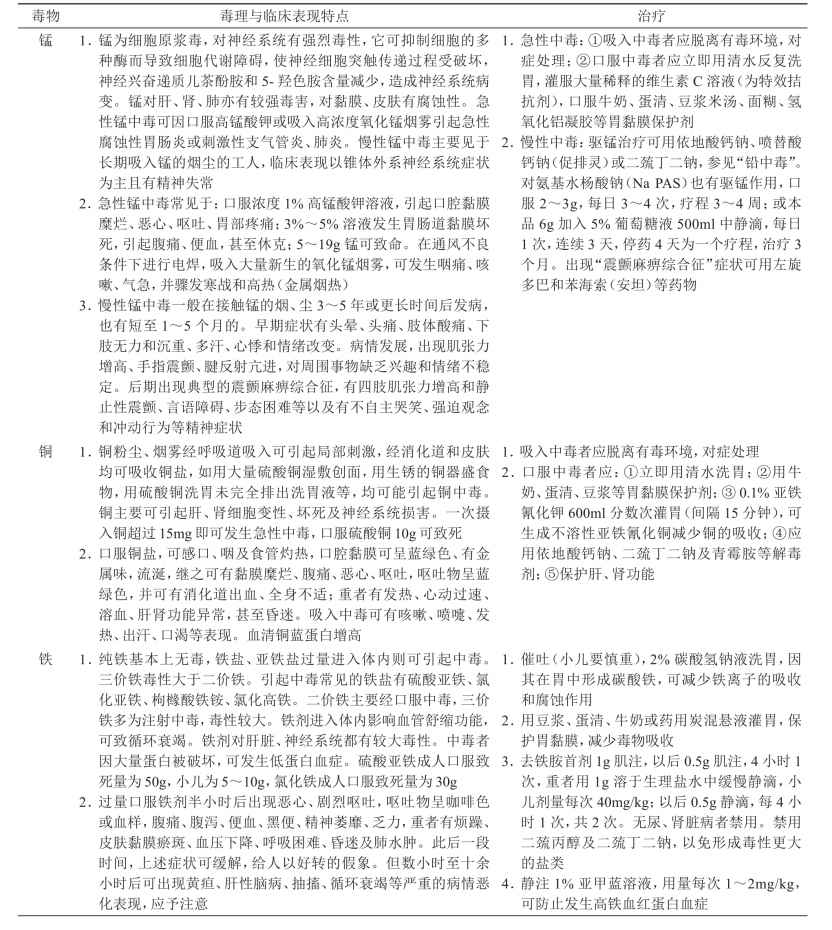
\includegraphics[width=\textwidth,height=\textheight,keepaspectratio]{./images/Image00219.jpg}\\
 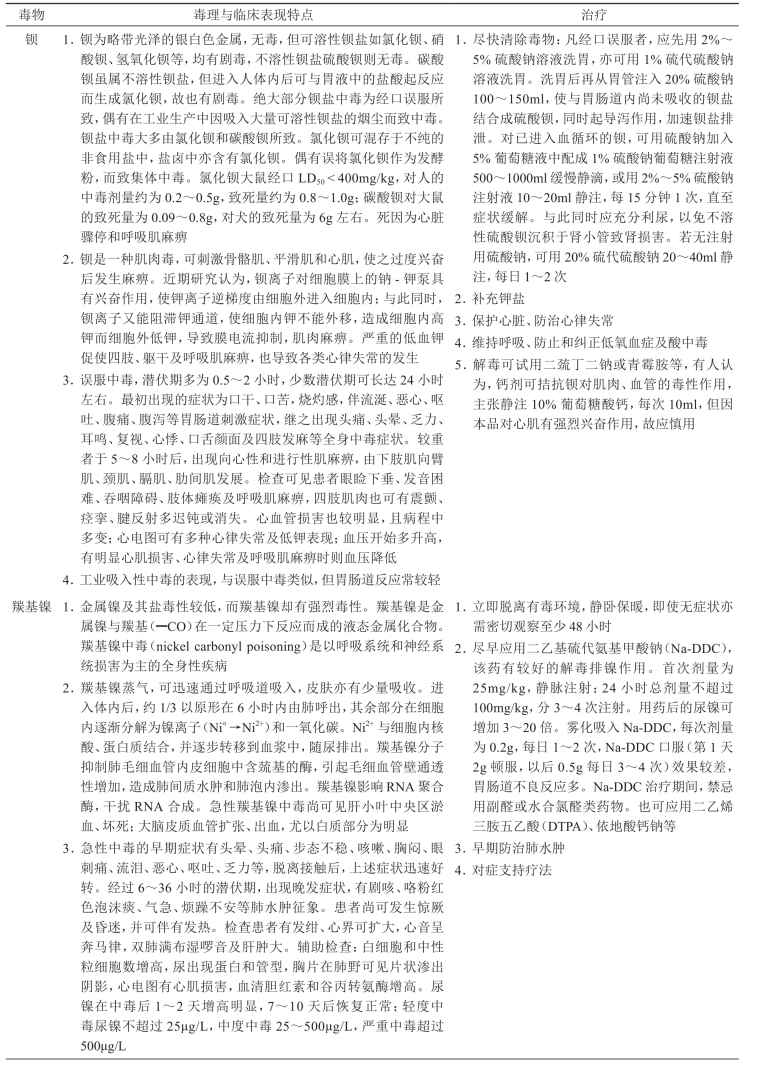
\includegraphics[width=\textwidth,height=\textheight,keepaspectratio]{./images/Image00220.jpg}\\
 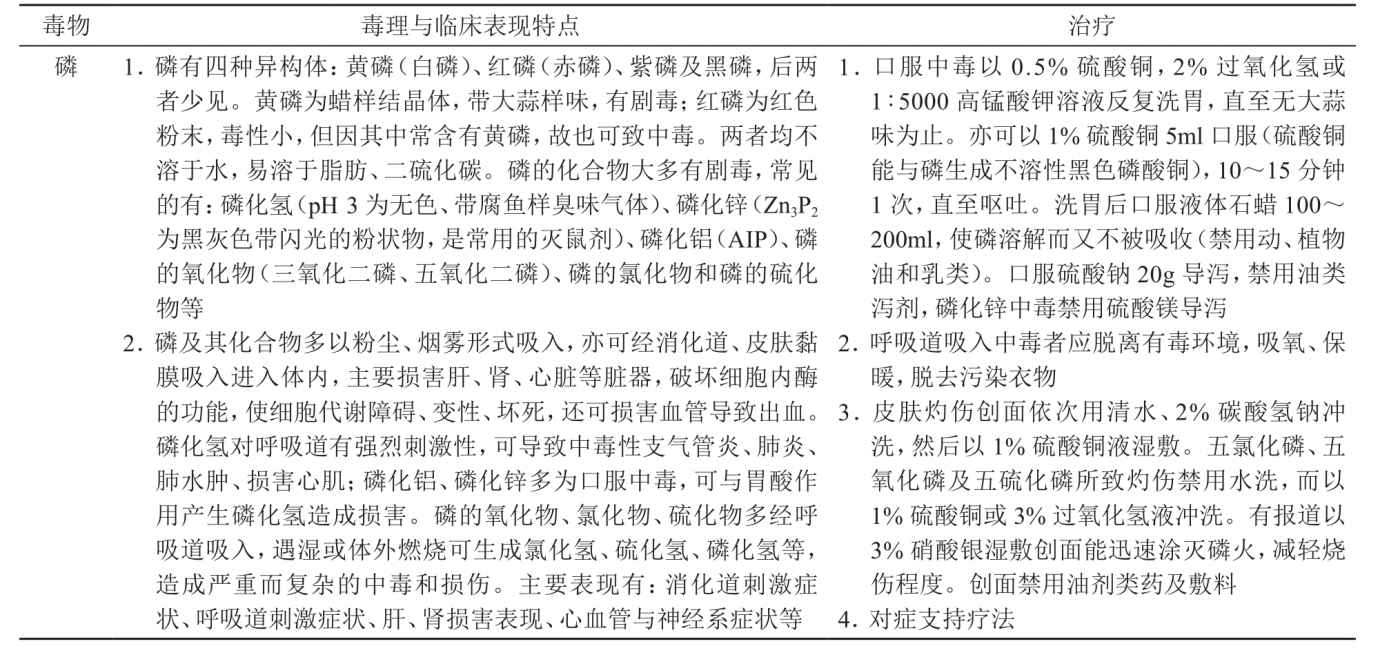
\includegraphics[width=\textwidth,height=\textheight,keepaspectratio]{./images/Image00221.jpg}
 \end{longtable}

\hypertarget{text00161.htmlux5cux23CHP5-6-5-1}{}
参 考 文 献

1. 陈灏珠 ,林果为.实用内科学.第13版.北京:人民卫生出版社,2009

2. 朱子扬,龚兆庆,汪国良.中毒急救手册.上海:上海科学技术出版社,2007

\protect\hypertarget{text00162.html}{}{}

\chapter{植物性毒物中毒}

\section{亚硝酸盐中毒}

\subsection{病因与中毒机制}

亚硝酸盐中毒(nitrite
poisoning)既往多是由进食较多含有硝酸盐的蔬菜和苦井水、蒸锅水等引起的肠源性发绀,近年来则多见因误将亚硝酸钠当作食盐使用而致中毒,且常为群体性中毒。

亚硝酸盐主要为亚硝酸钠(钾),多为白色结晶性粉末,味微咸或稍带苦味,易溶于水。工业上用亚硝酸钠作金属表面处理或用作某些有机物(如染料)合成的原料,罕有发生中毒者。亚硝酸钠(钾)也用于食品加工及防腐,可因误用误食而致急性中毒。某些蔬菜如青菜、小白菜、韭菜、卷心菜、莴苣、甜菜、菠菜、萝卜叶等,野菜如灰菜、荠菜均含有丰富的硝酸盐(50~150mg/dl)和微量的亚硝酸盐(0.2~0.5mg/dl),新鲜腌渍的咸菜和变质熟剩菜,由于硝酸盐还原菌的作用,使其所含的无毒的硝酸盐还原为有毒的亚硝酸盐(其含量可高达5mg/dl以上),食用此类蔬菜后可引起中毒;其次当肠道功能紊乱、胃酸减少等原因,使肠内硝酸盐还原菌(其中大肠埃希菌和沙门菌还原硝酸盐为亚硝酸盐的能力最大)大量繁殖,能使大量硝酸盐还原为亚硝酸盐,因此更易引起中毒;大量饮用硝酸盐含量过高的井水(尤其是苦井水)、果实、蒸锅水,或是腌咸肉或烧煮卤味时加亚硝酸盐过多(硝肉),食后也可引起中毒。此外,营养不良、贫血、寄生虫感染等与硝酸盐类的还原均有密切关系。

亚硝酸盐毒性较大,摄入量达0.2~0.5g时即可引起中毒,最小致死量为1.0~5.0g。由于亚硝酸盐与血红蛋白的作用,使正常的Fe\textsuperscript{2+}
氧化成Fe\textsuperscript{3+}
,形成高铁血红蛋白而失去携氧能力;同时还阻止正常HbO\textsubscript{2}
释放氧,因而造成了各种组织的缺氧。临床上突出表现为皮肤、黏膜呈青紫色及其他缺氧症状,且与肠源性有关,故又名肠源性青紫症。口服亚硝酸钠部分于胃中转化为亚硝酸,后者再分解释出一氧化氮,引起胃肠道刺激症状。亚硝酸钠对中枢神经系统,尤其对血管舒缩中枢有麻痹作用,它还能直接作用于血管平滑肌,有较强的松弛作用而致血压降低。

\subsection{诊断}

\paragraph{病史}

有误食误用亚硝酸盐制剂如亚硝酸钠史,或有进食大量上述蔬菜和饮用含亚硝酸盐的井水史。多见于儿童及胃肠功能不全者,春季发病较多。同食者多人出现相似中毒症状。

\paragraph{临床表现特点}

发病常急骤,多在食后0.5~3小时发病(短者仅10~15分钟,长者可达20小时)。主要中毒症状为缺氧表现,如头晕、头痛、乏力、心慌、气促、恶心、呕吐及发绀(尤以口唇、指端更明显);继而可出现烦躁、嗜睡、呼吸困难、血压降低、肺水肿、心律失常、惊厥、昏迷、呼吸与循环衰竭。临床表现与高铁血红蛋白浓度有关:高铁血红蛋白达血红蛋白总量的10\%~15\%时,口唇、指甲及全身皮肤黏膜呈紫黑色、蓝灰或蓝褐色,与呼吸困难不成比例;高铁血红蛋白达30\%以上时,主要表现为头痛、头晕、耳鸣、心动过速、反应迟钝,精神萎靡、乏力等;升至50\%时,患者可有心悸、气急、恶心、呕吐、腹痛腹泻、心动过速、出冷汗等;如进一步增加,患者可发生休克、心律失常、肺水肿、惊厥甚至昏迷,如不及时抢救,可危及生命。

若患者同时有沙门菌和致病性大肠埃希菌感染,则可合并存在亚硝酸盐食物中毒和细菌性食物中毒,诊断时应予注意。还应注意排除苯的胺基和硝基化合物,农药杀虫脒、氯酸钠、除草醚等能引起高铁血红蛋白血症的化合物中毒。血高铁血红蛋白的测定有助于急性亚硝酸盐中毒的诊断,确诊有赖呕吐物或食物中亚硝酸盐的检测。

\subsection{治疗}

\paragraph{一般处理}

置患者于空气新鲜而通风良好的环境中,吸氧,并使患者绝对卧床休息,注意保暖。如此,轻症患者(高铁血红蛋白量在30\%以下)便能自行恢复,因高铁血红蛋白大都能在24~48小时内完全转变为Hb之故。

\paragraph{清除毒物}

误服亚硝酸盐应及早洗胃及导泻,现场不能洗胃者,只要神志清楚,宜先作催吐。如中毒时间较长,可配合高位灌肠以清除残存毒物。

\paragraph{特效疗法}

①亚甲蓝(美蓝)的应用:用法为1\%亚甲蓝1~2mg/kg溶入25\%~50\%葡萄糖液20~40ml,于10~15分钟内缓慢静注,如症状仍不缓解,2小时后可重复一次。使用亚甲蓝时需用小剂量,因为小剂量亚甲蓝进入机体后即被组织内的还原型辅酶Ⅰ脱氢酶还原为还原型亚甲蓝,起到还原剂的作用,使高铁血红蛋白还原为Hb,从而改善缺氧状态;当大量亚甲蓝快速进入人体后,还原型辅酶Ⅰ脱氢酶不能使其全部还原为还原型亚甲蓝,此时亚甲蓝则为氧化剂,可直接将Hb氧化为高铁血红蛋白,故应特别注意。②应用高渗葡萄糖液和大剂量维生素C:适用于轻症患者及重症患者的辅助治疗。如用50\%葡萄糖液60~100ml加维生素C
1~2g静注,或用维生素C
2~4g加入10\%葡萄糖液500~1000ml中静滴。维生素C可使高铁血红蛋白还原为Hb,而脱氢的维生素C又被谷胱甘肽还原,以后又作用于高铁血红蛋白,如此反复不已,使血液中高铁血红蛋白浓度降低,但其作用不如亚甲蓝迅速和彻底。注射葡萄糖的目的,则为利用其氧化作用,以提高高铁血红蛋白还原过程中所需要的NADPH,故可作为治疗辅助剂。辅酶A和维生素B\textsubscript{12}
也有辅助作用。

\paragraph{对症支持疗法}

包括防治休克与呼吸衰竭等,有意识障碍、昏迷者加用纳洛酮治疗。病情危重经上述处理后发绀仍明显者,可输新鲜血300~500ml,或行换血疗法。

\protect\hypertarget{text00163.html}{}{}

\section{毒蕈中毒}

毒蕈又称毒蘑菇,在自然界分布很广。全世界毒蘑菇约200余种,我国已知的毒蘑菇有190多种,能致死的达30余种。常由于不少毒蘑菇与食用蘑菇不易区别而误食中毒,城市居民中则多因食用混杂的干蘑菇而发生毒蕈中毒(mushroom
poisoning)。

\subsection{病因与中毒机制}

不同类型的毒蘑菇含有不同的有毒成分,但一种毒蘑菇也可含有多种毒素,而有时多种毒蘑菇可同含一种毒素。主要有毒成分可分为以下几类:

\paragraph{肝脏毒素}

有毒肽、毒伞肽二种,后者的毒性是前者的20倍。该类毒素可致肝脏急性炎症、坏死,肝细胞空泡变性及灶性出血,同时可致胃肠道充血、水肿、出血;急性肾小管变性及坏死;心脏细胞肿胀、脂肪变性;脑水肿、充血及点状出血。肝脏毒素含于毒伞(amanita
phalloides)、白毒伞(amanita verna)、鳞柄毒伞(amanita
virosa)等毒蕈中。

\paragraph{神经、精神毒素}

有毒蝇碱、异{} 唑类衍生物、蟾蜍素和光盖伞素4种。主要含于毒蝇伞(amanita
muscaria)、豹斑毒毒伞(amanita pantherina)、角鳞灰伞(amanita
spissacea)及牛肝蕈(boletus)等毒蕈中。蝇碱作用类似乙酰胆碱,阿托品有拮抗作用,是有效的解毒剂。异{}
唑类衍生物包括毒蝇母、白蘑酸、麦萨松等,主要作用于中枢神经系统。蟾蜍素及光盖伞素主要引起幻想、幻视、哭笑无常等精神症状。

\paragraph{胃肠毒素}

此类毒素有胍啶和蘑菇酸等,含于毒粉褶蕈(rhodophyllus
sinuatus)、毒红菇(russlaemetica)、毛头乳菇(lacfarius
forninosis)、墨汁鬼伞(caprinus atramentarius)、红网牛肝蕈(boletus
luridus)及虎斑口蘑(tricholoma
tigrinum)等毒蕈中。是引起胃肠炎症状的毒素,对胃肠道有刺激作用。

\paragraph{溶血毒素}

主要毒蕈有鹿花蕈(gyromitra esculenta)、纹缘毒伞(amanita
spreta)等,所含毒素有鹿花蕈素、毒伞溶血素等,可引起溶血。

\subsection{诊断}

\subsubsection{病史}

有进食干蕈史,是诊断毒蕈中毒的重要依据。由于本病发病时多有吐泻症状,如不注意询问食蕈史常易误诊为胃肠炎、菌痢或一般食物中毒等,故当遇此类患者,尤在夏秋季节呈一户或数户人同时发病者,应想到本病的可能性。如能从现场觅得毒蕈加以鉴定,则诊断更臻完善。

\subsubsection{临床表现特点}

由于每种毒蕈所含毒素不一,中毒的临床表现也各异,按主要表现大致可分为胃肠炎型、神经精神型、溶血型和中毒性肝炎型4型:

\paragraph{胃肠炎型}

几乎所有毒蕈中毒首先表现为轻重不一的胃肠炎。致严重胃肠炎的毒蕈有毒粉褶菌、小毒蝇菇(amanita
mellaiceps)、黄粘盖牛肝(suillus placidus)、密褶黑菇(russula
densifolid)、肥脚环柄菇等。潜伏期0.5~1小时,表现为恶心、呕吐、腹痛、腹泻、头晕、头痛,可伴有水和电解质失衡与周围循环衰竭。患者可因失水、电解质失衡、昏迷、休克致死。但单纯胃肠炎型毒蕈中毒经积极治疗后可迅速恢复,死亡率极低。

\paragraph{神经精神型}

由误食毒蝇伞(amanita muscaria)、豹斑毒伞(amanita
pantherina)、红网牛肝(boletus luridus)、毒红菇(russula
emetica)、光盖伞属(psilocybe)、假黑伞属(stropharia)、细网牛肝(boletus
satanas)等毒蕈所引起。毒性物质有毒蝇碱、蟾蜍素、光盖伞素等。潜伏期约1~6小时,临床表现除胃肠炎外,尚有副交感神经兴奋症状,如多汗、流涎、流泪、脉缓、瞳孔缩小等;阿托品类药物疗效甚佳。少数病情严重者出现头昏、谵妄、幻觉,甚至被迫害妄想,以致发生自杀或杀人行为,或类似精神分裂症表现。个别患者发生癫痫大发作。经过积极治疗,很快康复,死亡率甚低。

\paragraph{溶血型}

因误食鹿花蕈(gyromitra esculenta)、纹缘毒伞(amanita
spreta)等所引起。所含毒素有鹿花蕈素、毒伞溶血素等。潜伏期6~12小时。除引起胃肠炎症状外并引起溶血,导致贫血、肝脾肿大等。对中枢神经系统也有影响,可产生头痛等症状。给予皮质激素及输血等治疗多可康复,死亡率一般不高。

\paragraph{中毒性肝炎型}

因误食毒伞(amanita phalloides)、白毒伞(amanita
verna)、鳞柄毒伞(amanita
virosa)等所引起。其所含毒素包括毒伞肽(amatoxins)和毒肽(phallotoxin)两大类共11种化学结构,为环肽类中分子物质,耐热、耐干燥,不为一般烹调所破坏。毒肽主要作用于肝细胞内质网,发生作用快,大剂量摄入1~2小时内可致死;毒伞肽作用较迟缓,但毒性较毒肽大20倍,能直接作用于细胞核,有可能抑制RNA聚合酶,并能显著减少肝糖原而导致细胞迅速坏死,并兼有肾脏、心脏和神经毒作用,摄入0.1mg/kg以下即可致死。此型中毒病情凶险,如无积极治疗死亡率可高达50\%~90\%。此型临床过程可分为以下6期:

\hypertarget{text00163.htmlux5cux23CHP5-7-2-2-2-4-1}{}
(1) 潜伏期:

6~48小时,多在24小时内发病。

\hypertarget{text00163.htmlux5cux23CHP5-7-2-2-2-4-2}{}
(2) 胃肠炎期:

患者可突然发生上腹部和腹部剧烈疼痛,随之出现与胃肠炎型相同的表现。症状持续1~2天缓解。

\hypertarget{text00163.htmlux5cux23CHP5-7-2-2-2-4-3}{}
(3) 假愈期:

胃肠炎症状自行缓解后,患者无明显症状,给人以病愈感觉。此期内进入脏器的毒素与靶细胞结合,逐渐损害脏器实质,导致进行性功能障碍。轻型患者肝损害不严重,可由此进入恢复期。

\hypertarget{text00163.htmlux5cux23CHP5-7-2-2-2-4-4}{}
(4) 内脏损害期:

中毒后1~5天(平均2~3天)出现以肝、肾、脑、心为主的内脏损害,肝脏损害最为严重,多表现为肝肿大、黄疸、肝功改变,转氨酶增高,可导致急性或亚急性肝坏死,肝缩小,黄疸加深、烦躁、意识模糊,甚至出现肝昏迷。可并发DIC。肾脏可同时受累,发生肾功能衰竭。

\hypertarget{text00163.htmlux5cux23CHP5-7-2-2-2-4-5}{}
(5) 精神症状期:

多在内脏损害后出现。患者烦躁不安、谵语、抽搐、惊厥、昏迷,多死于呼吸衰竭。部分患者出现精神失常,时哭时笑,日后逐渐安定。

\hypertarget{text00163.htmlux5cux23CHP5-7-2-2-2-4-6}{}
(6) 恢复期:

经2~3周后,患者肝功能好转,症状逐渐减轻,4~6周多能痊愈。

部分病例于食后6小时发病,病情迅速恶化,初为胃肠道症状,继则出现休克、抽搐、呼吸衰竭、全身广泛性出血、昏迷等症状,称暴发型,常于1~2天内突然死亡。这可能与急性肝坏死、高度脑水肿、中毒性心肌病及全身广泛出血等严重中毒损害有关。

最近,有学者根据对172例临床资料及文献报道的分析,提出分为胃肠炎型、急性肾功能衰竭型、中毒性肝炎型和混合型等四型。

\subsection{治疗}

\paragraph{清除毒物}

应及时采用催吐、洗胃、导泻、灌肠等方法以迅速排除尚未吸收的毒物。尤其对误食毒伞、白毒伞等毒蕈者,其发病虽较迟缓,就诊时距食蕈常已在6小时以上,但上述治疗仍有重要意义。催吐可应用人工刺激咽部,或用阿扑吗啡(但5岁以下儿童及昏迷患者禁用)。选用1∶5000高锰酸钾溶液、3\%~5\%鞣酸溶液或0.5\%活性炭混悬液等反复洗胃。无腹泻者,于洗胃完毕可经口服硫酸钠20g导泻。如中毒时间已超过8小时,可用温盐水行高位结肠灌洗,每次200~300ml,连续2~3次。如患者已有严重的呕吐和腹泻,则不必催吐和导泻。

\paragraph{血液净化疗法}

血液净化治疗毒蕈中毒,疗效较肯定,且可治疗并发的急性肾功能衰竭和水、电解质、酸碱平衡失调。对中、重型中毒患者尽早采用血液灌流或血液透析治疗。

\paragraph{抗胆碱药}

主要用于含毒蕈碱的毒蕈中毒,可解除副交感神经过度兴奋症状,对中毒性心肌炎所致的房室传导阻滞(AVB)和中毒性脑炎所致的呼吸中枢衰竭具有治疗作用。可根据病情用阿托品0.5~2mg皮下注射,每0.5~6小时一次,必要时可加大剂量或改用静注,直至瞳孔扩大、心率增快、面色潮红、症状缓解。此后逐渐减量和延长间隔时间。

\paragraph{巯基解毒药}

用于中毒性肝炎型毒蕈中毒患者,即使在假愈期没有明显内脏损害时,也应给予此药。其作用机制可能是含巯基的药物与某些毒素如毒伞肽等相结合,打断了其分子中的硫醚键,使其毒力减弱。而保护了体内含巯基酶的活性,甚至恢复部分已与毒素结合的酶的活力。由于患者肝脏损害多数严重,故不宜用二巯丙醇。常用的有:①二巯丁二钠(DMS):0.5~1g稀释后静脉注射,每6小时1次,首剂加倍,症状缓解后改为每日注射2次,连用5~7天为1疗程。②二巯丙磺钠:5\%溶液5ml肌肉注射,每6小时1次,症状缓解后改为每日注射2次,至5~7天为1疗程。

\paragraph{肾上腺皮质激素}

适用于溶血型毒蕈中毒及其他重症的中毒病例,尤其是有中毒性心肌炎、中毒性脑炎、严重的肝损害和出血倾向的病例。如用氢化可的松200~300mg/d或地塞米松10~20mg/d加入液体中静滴,病情好转后改用泼尼松口服。

\paragraph{抗蕈毒血清的应用}

对于白毒伞等毒性很强的毒蕈中毒,有条件时可用抗蕈毒血清治疗。

\paragraph{对症支持疗法}

吐泻剧烈者,应大量补液,在保持水、电解质平衡的前提下,可给予利尿剂,使毒素从尿中大量排出。对有肝损害者应给予保肝支持治疗如用肝细胞生长素,促进受损肝细胞的修复。对有精神症状或有惊厥者应予镇静或止惊药物治疗,并可试用脱水剂。

\protect\hypertarget{text00164.html}{}{}

\section{乌头碱类植物中毒}

乌头(aconitum
carmichaelii)属毛茛科,主根为乌头,支根为附子。同科野生的有草乌头、一枝篙、落地金钱、搜山虎。乌头全株有毒,毒性依次为根、种子、叶。草乌头等比乌头毒性更大。一般中毒剂量:附子30~60g、川乌3~90g、草乌3~4.5g、一枝篙0.5~3g、落地金钱1~2.5g、搜山虎3g。但人体对乌头碱可有耐受性,长期运用可使中毒量提高。乌头类植物其有毒成分系乌头碱(aconitine),口服0.2mg即能使人中毒,口服3~5mg即可致死。乌头碱经煎煮,水解成毒性较弱的苯酰乌头原碱和乙酸;苯酰乌头原碱又可进一步水解成毒性极微的乌头原碱和苯甲酸。因此,煎煮时时间越长,毒性越低,一般煎煮3~4小时后,乌头碱几乎全部破坏。临床上常因对乌头生药的炮制或水煎不当而服用,引起中毒。

\subsection{病因与中毒机制}

乌头碱能通过消化道或破损皮肤吸收,主要经肾脏及唾液排出。因吸收快,故中毒极为迅速,可于数分钟内出现中毒症状。乌头碱主要作用于神经系统,使之先兴奋后抑制,甚至麻痹;感觉神经、横纹肌、血管运动中枢和呼吸中枢可麻痹。乌头碱还可直接作用于心肌,并兴奋迷走神经中枢,致使心律失常及心动过缓等。

\subsection{诊断}

\paragraph{病史}

有用乌头碱类植物史。

\paragraph{临床表现特点}

口服中毒者,首先表现口腔及咽部黏膜刺痛及烧灼感,舌及口腔周围有麻木感,言语笨拙。当药物被吸收后约0.5小时即可出现下述症状:①神经系统:四肢麻木,特异性刺痛及蚁行感,麻木从上肢远端(指尖)开始向近端蔓延,继后为口、舌及全身麻木,痛觉减弱或消失,有紧束感。伴有眩晕、眼花、视物模糊。重者躁动不安、肢体发硬、肌肉强直、抽搐,意识不清甚至昏迷。②循环系统:由于迷走神经兴奋及心肌应激性增加,可有心悸、胸闷、心动过缓、多源性和频发室性期前收缩、心房或心室颤动或阿-斯综合征等多种心律失常和休克。③呼吸系统:呼吸急促、咳嗽、血痰、呼吸困难、发绀、急性肺水肿,可因呼吸肌痉挛而窒息,甚至发生呼吸衰竭。④消化系统:恶心、呕吐、流涎、腹痛、腹泻、肠鸣音亢进,少数有里急后重、血样便、酷似痢疾。

\subsection{治疗}

乌头口服中毒者应立即用1/5000高锰酸钾、2\%食盐水或浓茶反复洗胃,洗胃后可灌活性炭30~50g,随后再灌入硫酸钠20~30g导泻。静脉补液,以促进毒物的排泄。同时,注射阿托品,有抑制腺体分泌、解除平滑肌的过度紧张状态、阻断迷走神经对心脏的影响及兴奋呼吸中枢的作用。一般用1~2mg皮下或肌肉注射,每4~6小时1次;对重症者可酌情增大剂量及缩短间隔时间,必要时可用0.5~1mg静注。如在应用阿托品后,仍有频发室性期前收缩、阵发性室性心动过速等,可选用利多卡因、胺碘酮、普罗帕酮等纠正之。如有呼吸衰竭及休克,应及时给予吸氧、呼吸兴奋剂、人工呼吸及抗休克治疗等。

\protect\hypertarget{text00165.html}{}{}

\section{发芽马铃薯中毒}

\subsection{病因与中毒机制}

马铃薯(solanum
tuberosum)俗称土豆(potato)、山药蛋、洋山芋等,为人们普遍食用食物。未成熟或发芽的块根含有毒物质为龙葵碱、毒茄碱、胰蛋白酶、糜蛋白酶、胞质素和细胞凝集素等,而以龙葵碱最为重要。人食入龙葵碱0.2~0.4g即可引起中毒。它是一种弱碱性的苷生物碱。每100g马铃薯含龙葵碱仅5~10mg;未成熟、青紫皮的马铃薯或发芽马铃薯含龙葵碱增至25~60mg,甚至高达430mg。该毒素可溶于水,遇醋酸极易分解,高热煮透亦可破坏其毒性,因而只有吃了未经妥善处理的发芽马铃薯或不成熟马铃薯才易中毒。龙葵苷对胃肠道黏膜有较强的刺激性及腐蚀性,对中枢神经系统有麻痹作用,尤其对呼吸中枢及运动中枢作用明显。此外对红细胞有溶解作用,可致溶血。其病理变化主要为急性肺水肿,其次为胃肠炎及肺、肝、心肌和肾脏皮质的水肿等。

\subsection{诊断}

\paragraph{病史}

有进食发芽或未成熟马铃薯史。

\paragraph{临床表现特点}

一般在食后0.5~2小时发病。先有咽喉及口内刺痒或灼热感,继有恶心、呕吐、腹痛、腹泻等症状。轻者1~2天自愈;重者因剧烈呕吐而有失水及电解质紊乱,血压下降;严重中毒患者有昏迷及抽搐,最后因呼吸中枢麻痹而导致死亡。

\paragraph{实验室检查}

将剩余的马铃薯切开,在芽附近加浓硫酸或浓硝酸数滴,如变为玫瑰红色即证明有毒素存在。

\subsection{治疗}

发芽马铃薯中毒无特效疗法,主要是对症处理。发现中毒后应立即用1∶5000高锰酸钾或0.5\%鞣酸溶液或浓茶洗胃,硫酸钠导泻。补充液体纠正失水。呼吸困难时积极给氧和应用适量呼吸兴奋剂。呼吸中枢麻痹用人工呼吸机。在预防中毒方面,未成熟青紫皮和发芽马铃薯不可食用;少许发芽马铃薯应深挖去发芽部分,并浸泡半小时以上,弃去浸泡水,再加水煮透,倒去汤汁才可食用;在煮马铃薯时可加些米醋,因其毒汁遇醋酸可分解,变为无毒。

\protect\hypertarget{text00166.html}{}{}

\section{霉变甘蔗中毒}

甘蔗(cane)味甜可口,人们多喜爱,儿童尤甚。但若误食霉变甘蔗(moldy
sugar
cane)则致中毒,常能危及生命或留有神经系统后遗症,病死率在10\%以上,重症可达40\%。

\subsection{病因与中毒机制}

霉变甘蔗的发生多由于长期贮存,越冬出售,受冻后化冻,在适宜温度下,真菌繁殖。未成熟甘蔗更易发生霉变。霉变甘蔗含糖量低,具酸霉味、酒糟味,食用后便可引起中毒,多见于儿童。目前认为导致霉变甘蔗中毒的病原是节菱孢菌(Arthrinium
spp),其所产生的毒素为3-硝基丙酸(3-nitropropionic
acid,3-NPA)。3-NPA为一种神经毒素,进入人体后迅速吸收,短时间内引起广泛性中枢神经系统损害,干扰细胞内酶的代谢,增强毛细血管的通透性,从而引起脑水肿、脑疝等。严重者导致缺血坏死,出现各种有关的局灶症状。有些损害为不可逆性。

\subsection{诊断}

多在食后15分钟~8小时内发病,亦有长至48小时。潜伏期愈短,症状愈重,预后愈差。

\paragraph{轻度中毒}

首先表现为一时性胃肠道功能紊乱(恶心、呕吐、腹痛等,无腹泻),并可出现神经系统症状(头痛、头晕、眼前发黑、复视),轻者很快恢复,较重者胃肠道症状加重,频繁恶心、呕吐,并可发生昏睡。

\paragraph{重度中毒}

在上述症状出现后,很快出现抽搐、昏迷。抽搐表现为阵发性痉挛性,每次发作1~2分钟,每日可多次发作。抽搐发作后便呈昏迷状态,且眼球向上看,瞳孔散大。尚可发生急性肺水肿和血尿。体温初期正常,3~5天后可升高。一般在5~10天后疾病开始恢复。可有神经系统后遗症如全身性痉挛性瘫痪、去大脑皮质综合征等。

\paragraph{辅助检查}

CT扫描轻症患者大都正常,重症患者在亚急性期可见双侧苍白球、壳核、尾状核、豆状核等部位呈现低密度区,间以片状出血;后期可见弥漫性脑萎缩。脑电图可有广泛的轻、中度异常。

\subsection{治疗}

1.清除毒物 用清水、生理盐水或0.5\%药用炭混悬液洗胃,导泻。

2.对症支持疗法
静脉输液,给予大剂量维生素C及B族维生素,维持水、电解质平衡,保护肝、肾功能。应用糖皮质激素减轻中毒反应,增强机体应激性,可用氢化可的松200~300mg静滴,每日1次。应用脱水剂防治脑水肿、改善脑细胞代谢的药物的应用等。

3.高压氧疗法。

\protect\hypertarget{text00167.html}{}{}

\section{菜豆角中毒}

\subsection{病因与中毒机制}

菜豆角又称梅豆角、四季豆、扁豆、刀豆、肉豆、泥鳅豆、豆角等。其含的毒性物质包括:①豆素:为一种毒蛋白,含于各种食用豆类中,具有凝血作用,须经长时间煮沸才可破坏;②皂素:对黏膜有强烈的刺激性,并含有能破坏红细胞的溶血素。此种毒素常含于豆荚(外面的皮)中。此外,菜豆角若放置24小时或更久,其亚硝酸盐的含量大为增加,后者使血液中的Hb形成大量的高铁Hb,不能与氧结合而失去携氧能力,导致全身缺氧、发绀等。

\subsection{诊断}

\paragraph{病史}

急性中毒大多发生在秋季,常因进食大量贮存过久、烧煮不透的菜豆角所致。

\paragraph{临床表现特点}

潜伏期1~5小时。主要表现有恶心、呕吐、腹痛、腹泻、腹胀、头痛、头晕,部分患者有胸闷、心悸、出冷汗、四肢麻木、畏寒等。由于菜豆角所含的皂素须在100℃以上才能破坏,故在食用前未经充分烧煮,进入胃肠道后,即对胃肠黏膜发生强烈的刺激作用,呕吐、腹泻明显,减少了毒素吸收,故中毒表现为发病急骤、病程较短、预后较好,很少出现溶血或凝血现象。

\subsection{治疗}

主要是对症支持治疗。呕吐、腹泻不重者,可以催吐、洗胃及导泻。腹部绞痛可用维生素K\textsubscript{3}
8~16mg肌内注射。静脉输注5\%葡萄糖氯化钠溶液,以促进毒物排泄,维持水电解质平衡等。

\protect\hypertarget{text00168.html}{}{}

\section{白果中毒}

白果(semen
ginkgo)又名银杏,为银杏科落叶乔木银杏的种子,可以煮食或炒食,但不可生食。不论成人或小儿均可因食白果过量而致中毒,最小中毒量20粒,年龄愈幼、体质愈差、愈易中毒。婴儿连吃10粒左右即可致死,3~7岁小儿连吃30~40粒则致严重中毒,甚至死亡。成人如食入过量,亦可引起严重的高热、抽搐、肢体弛缓性瘫痪等中毒症状。

\subsection{中毒机制}

白果种子有毒,其毒性以其绿色的胚为最剧烈,其肉质外种皮含有毒成分为银杏酚、白果酚、白果酸、氢化白果酸、氢化白果亚酸等。种仁含微量的氰苷。肉质外种皮的液汁侵犯皮肤,可产生皮炎。白果所含的有机毒素能溶入水,毒性强烈。因其毒素遇热能减小毒性,故生食者中毒症状更著。中毒患者主要表现为中枢神经系统损害及胃肠道症状,偶可发生末梢神经受损表现。

\subsection{诊断}

\paragraph{病史}

有进食大量白果史。

\paragraph{临床表现特点}

中毒症状发生在进食白果1~12小时后,先有胃肠道症状如恶心、呕吐、腹痛、腹泻、食欲不振;随即有中枢神经系统症状如头晕、乏力、精神呆滞、反应迟钝、头痛、极度恐惧、怪叫、反复抽搐或惊厥、意识障碍等。接触核仁和肉质外皮可发生接触性皮炎。偶可发生末梢神经受损表现如触觉、痛觉消失、双下肢弛缓性瘫痪、膝腱反射迟钝或消失。重症患者尚可有气急、发绀、呼吸困难,常于1~2天内因心力衰竭、呼吸衰竭而危及生命。

\subsection{治疗}

主要是对症支持治疗。口服者立即催吐、洗胃、导泻。静脉输注5\%葡萄糖氯化钠溶液,以促进毒物排泄,维持水电解质平衡等。将患者置于安静室内,避免因各种刺激而引起惊厥。若已有惊厥不止,可予地西泮0.2~0.5mg/kg静脉注射;10\%水合氯醛0.5ml/kg保留灌肠。若有恐惧、怪叫等精神症状,可用氯丙嗪。在惊厥期内,避免应用中枢神经兴奋剂。

民间常用甘草绿豆汤治疗白果中毒。也可选用白果壳32~64g煎水内服,或用甘草15~32g煎服;或用生蛋清5~7个、活性炭20g用40℃以下温水200ml调服。

\protect\hypertarget{text00169.html}{}{}

\section{荔枝中毒}

\subsection{中毒机制}

因荔枝含有α-次甲基环丙基甘氨酸,具有降低血糖作用。因此,进食大量荔枝易致中毒,出现类似低血糖表现。还有认为荔枝含有某种毒素,连续大量食用,可导致肝脂肪变性而引起中毒症状。

\subsection{诊断}

\paragraph{病史}

有连续多日大量食用荔枝史。

\paragraph{临床表现特点}

以小儿多见。潜伏期数小时。患者多于下半夜至清晨突然发病,病情进展快,主要表现有头晕、乏力、出汗、心悸、面色苍白,部分患者有口干、饥饿感、腹痛、腹泻等症状,严重者有昏迷、抽搐、面肌或四肢瘫痪等。血糖降低。

\subsection{治疗}

快速静注25\%~50\%葡萄糖液40~60ml,继之静滴10\%葡萄糖液,尿量多时适当补钾。中毒早期(6小时内)可予1/5000高锰酸钾溶液洗胃。应用大剂量维生素B族药物。对症支持治疗。

\protect\hypertarget{text00170.html}{}{}

\section{其他植物性毒物中毒}

其他植物性毒物中毒如博落回、猫豆、油桐子、相思豆、马桑、樟树油、莽草子、苦楝、大麻子、鸦胆子、细辛、白芷、杜衡、甘遂(猫儿眼)、瓜蒂、荞麦花与荞麦苗、夹竹桃、棉子、巴豆、芦荟等,其诊治要点详见表\ref{tab59-1}。

\begin{longtable}{c}
 \caption{其他植物性毒物中毒的诊治要点}
 \label{tab59-1}
 \endfirsthead
 \caption[]{其他植物性毒物中毒的诊治要点}
 \endhead
 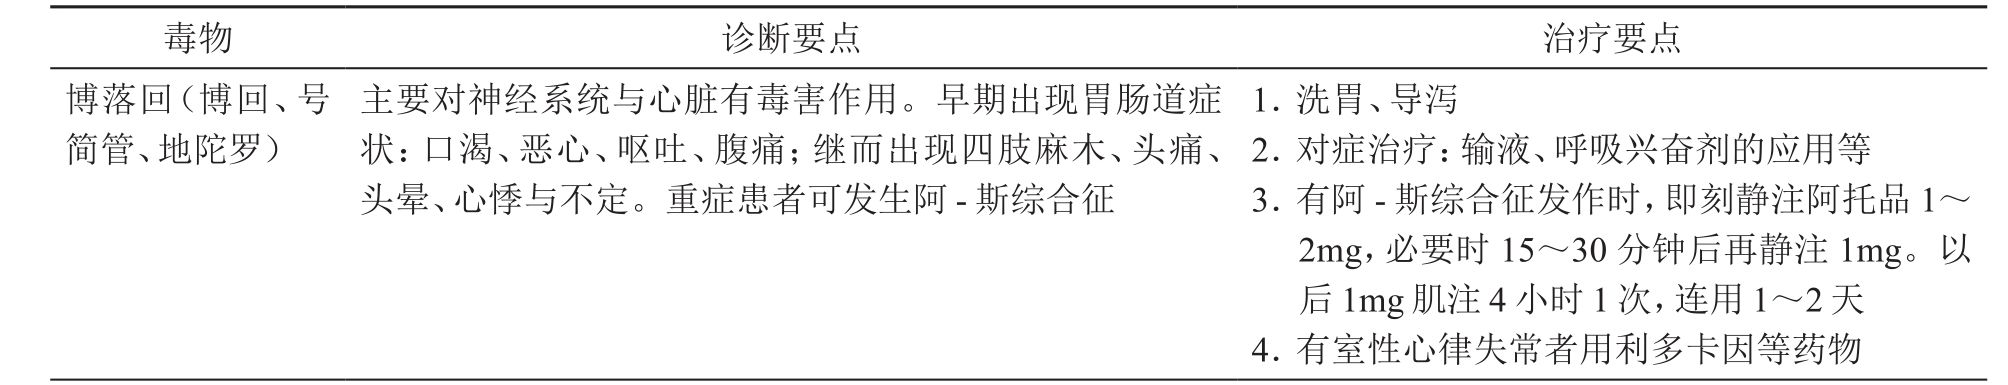
\includegraphics[width=\textwidth,height=\textheight,keepaspectratio]{./images/Image00224.jpg}\\
 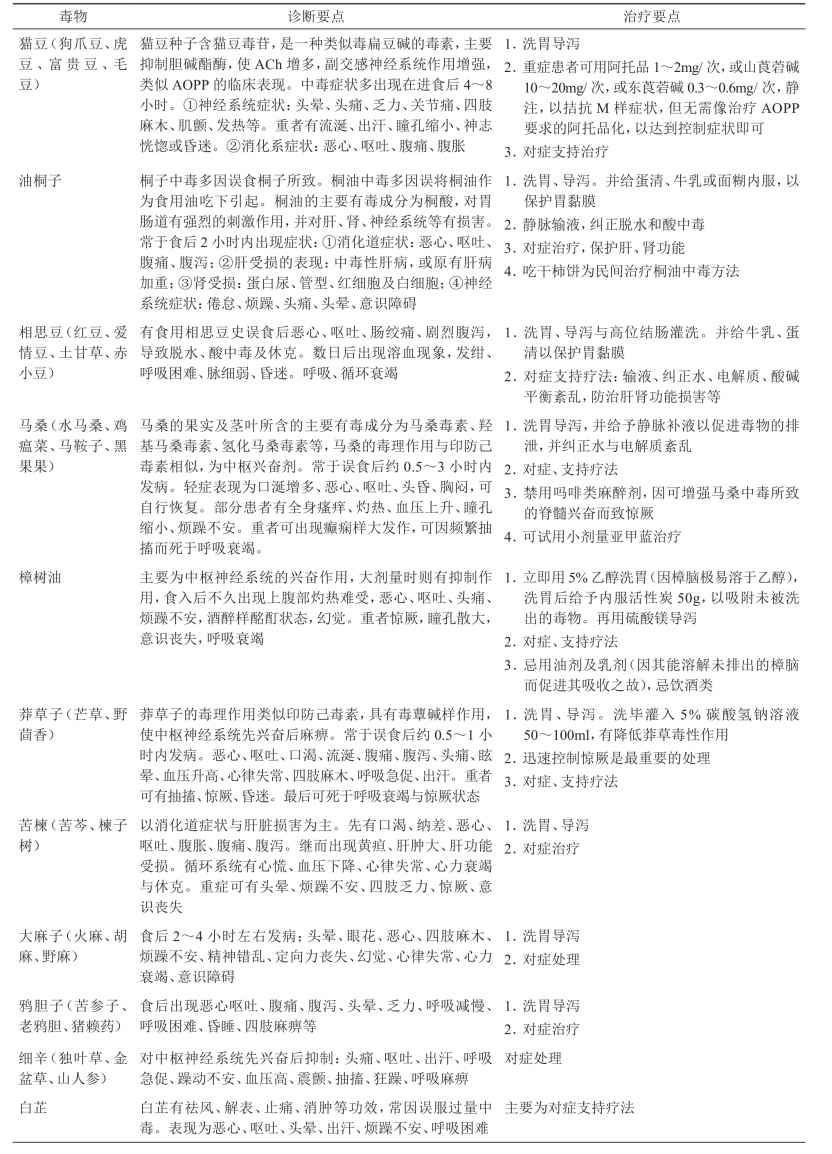
\includegraphics[width=\textwidth,height=\textheight,keepaspectratio]{./images/Image00225.jpg}\\
 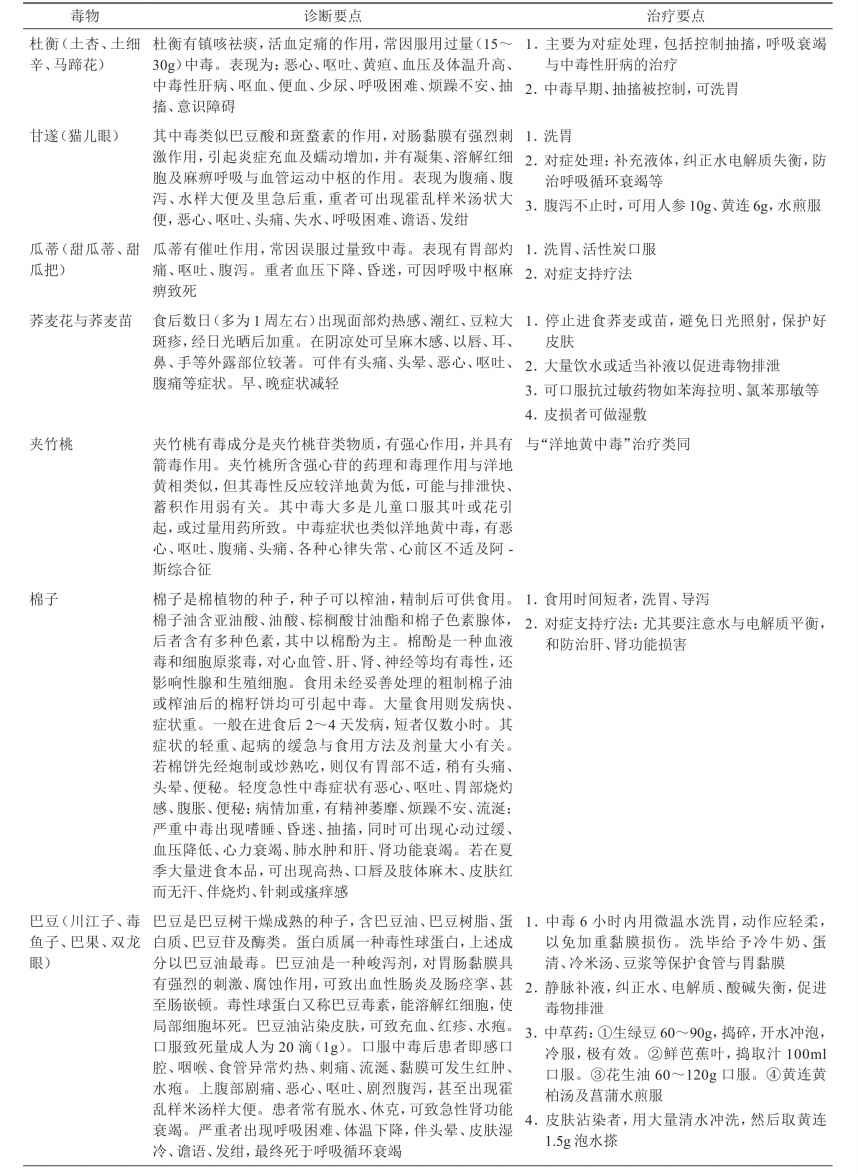
\includegraphics[width=\textwidth,height=\textheight,keepaspectratio]{./images/Image00226.jpg}\\
 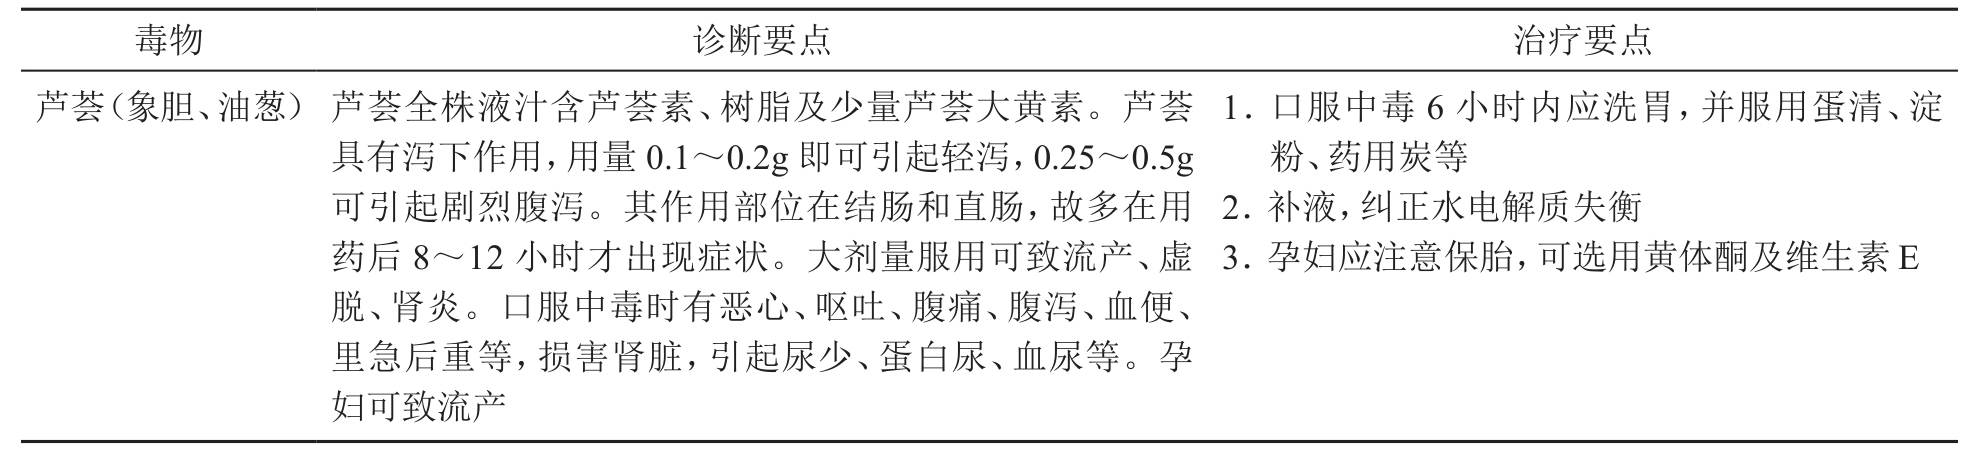
\includegraphics[width=\textwidth,height=\textheight,keepaspectratio]{./images/Image00227.jpg}
 \end{longtable}


\protect\hypertarget{text00171.html}{}{}

\hypertarget{text00171.htmlux5cux23CHP5-7-10}{}
参 考 文 献

1. 陈灏珠 ,林果为.实用内科学.第13版.北京:人民卫生出版社,2009

2. 朱子扬,龚兆庆,汪国良.中毒急救手册.上海:上海科学技术出版社,2007

3.
任成山,高全杰,陆海华,等.毒蕈中毒临床类型及特征分析.中国急救医学,2005,25(11):781

\protect\hypertarget{text00172.html}{}{}

\chapter{动物性毒物中毒}

\section{毒蛇咬伤}

我国各省都有蛇分布,大部分蛇种集中于长江以南、西南各省,已知蛇种209种,其中毒蛇有61种。毒蛇咬伤(venomous
snake
bites)是我国南方广大农村和山区的常见病,同时由于华南地区有食蛇的习惯,使整个蛇产业链都会出现蛇咬伤。自国家禁止吃野生动物后,因蛇产业接触出现的蛇伤病例明显减少。随着旅游业的发展,以及现在大型住宅区绿化率增加,因旅游和住宅区居民被蛇咬伤的病例也相应增多。

\subsection{病因与发病机制}

\subsubsection{毒蛇伤流行病学}

\begin{table}[htbp]
\centering
\caption{中国的毒蛇种属统计}
\label{tab60-1}
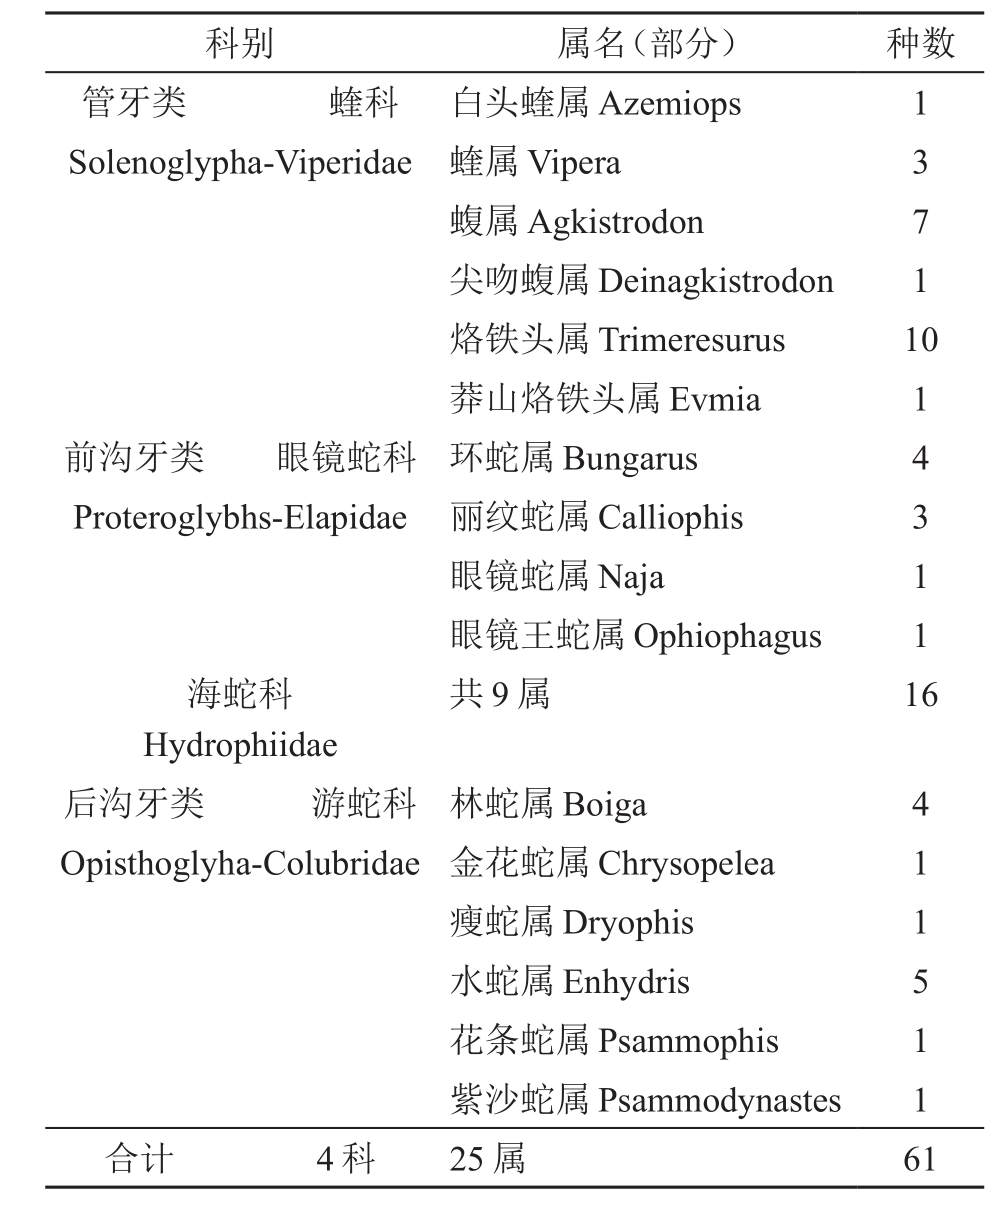
\includegraphics[width=3.3125in,height=4.01042in]{./images/Image00228.jpg}
\end{table}

中国的毒蛇种属统计见表\ref{tab60-1}。致伤蛇种随地区变化,广东以眼镜蛇、银环蛇、五步蛇、竹叶青蛇为主,广西以银环蛇为主,湘西以五步蛇为主,浙江以蝮蛇为主,青海目前只有蝮蛇。全国范围内以蝮蛇咬伤最多见,占57.69\%。近年出现了外国进口的蛇种,如泰国、印尼产的眼镜蛇、缅甸产的蝰蛇,由于种属的差异,一定程度上增大了蛇伤急救的难度。

毒蛇伤与气候、时间关系密切,春天后毒蛇伤病例增多同时病情也比较重,秋天后逐渐减少且病情相对比较轻,冬天因蛇要冬眠蛇伤则明显减少。白天多为眼镜蛇、眼镜王蛇及蝰蛇;晚上主要为银环蛇、金环蛇、烙铁头;晨昏时分多为竹叶青、蝮蛇、五步蛇、蝰蛇。

毒蛇伤男女比例:乡村为4~6∶1,城镇是8~10∶1。以青壮年为主。咬伤部位以四肢为主,特别下肢,占全部咬伤的70\%。

\subsubsection{毒蛇致伤机制}

毒蛇具有毒牙和毒腺(分泌毒液的器官)可以分泌出各自不同毒素性质的毒液,当毒蛇咬伤人体时,其毒液由沟牙或管牙注入人体,并经淋巴、血循环扩散,引起患者的局部和一系列的中毒症状。蛇毒经伤口吸收早期快,后期慢,咬伤局部组织中的蛇毒吸收呈“单峰长尾曲线”。

\subsubsection{蛇毒性质和毒理}

新鲜蛇毒为无色或淡黄色的半透明黏稠液体,有特殊腥味,含水量65\%~80\%,呈中性或弱酸性反应。大部分蛇毒加热后发生絮状沉淀,部分毒力会丧失,易受强酸、强碱、氧化剂(如高锰酸钾溶液等)及还原剂(如亚硫酸氢钠等)破坏;还易受蛋白水解酶类(如胰蛋白酶、链激酶、木瓜酶、α-糜蛋白酶等)所分解、破坏,减低毒性甚至失去毒力。蛇毒成分十分复杂,其质和量极不恒定,主要成分由多肽和酶类等毒性蛋白质组成,根据其毒理作用可概括为三类:

\hypertarget{text00172.htmlux5cux23CHP5-8-1-1-3-1}{}
(一) 神经毒素

神经毒素是蛇毒中毒性最强的一类
,可使被咬机体产生弛缓性麻痹和呼吸衰竭。主要存在于眼镜蛇科和海蛇科的毒液中,如银环蛇、金环蛇、海蛇等,眼镜蛇、眼镜王蛇也含有此毒素。神经毒素主要包括突触前神经毒素(pre-ATX)、突触后神经毒素(post-ATX)2种。突触前神经毒素又是毒性最强的神经毒素,主要作用于突触前膜K\textsuperscript{+}
通道,先导致乙酰胆碱(Ach)释放,再抑制其合成,最后阻断神经-肌肉(N-M)传导,其作用方式与肉毒杆菌的毒素作用相似。突触后神经毒素和神经-肌肉接头的烟酰胺型Ach受体有高度选择性结合的能力,使神经递质不能发挥作用,从而导致肌肉松弛,其原理与箭毒作用方式相似。

典型蛇种是银环蛇,其神经毒素含α、β、γ
3种蛋白组分,其中α属突触后神经毒素,β、γ属突触前神经毒素。三者共同作用,双重阻断了神经-肌肉接头的传递。神经毒素引起的骨骼肌弛缓性麻痹,按头、胸、膈肌、下肢顺序出现,反方向恢复。

\hypertarget{text00172.htmlux5cux23CHP5-8-1-1-3-2}{}
(二) 血循毒

血循毒主要存在于五步蛇
、蝰蛇、竹叶青蛇、烙铁头蛇的毒液中,眼镜蛇、蝮蛇也含有此毒素。血循毒的种类很多,成分复杂,产生多方面的毒性作用,主要以心血管和血液系统为主,导致凝血功能障碍,出现DIC和出血、纤溶等病理过程。

\paragraph{出血毒(BT)}

是主要的血循毒素,存在于蝰蛇科、眼镜王蛇毒液中。其中又含有抗凝因子和肌溶因子。引起机体血液凝固功能障碍、血管上皮损伤、结缔组织破坏和肌肉组织坏死。临床表现:在咬伤局部出现血疱、瘀斑、渗血不止、疼痛,能损伤小静脉、毛细血管引起血浆外渗、红细胞外漏而出血,甚至引起广泛的皮下、内脏出血和组织坏死。病情发展迅速是出血毒中毒的特点。

\paragraph{膜毒素(MT)}

各科毒蛇均存在,以眼镜蛇毒含量多。其命名常以主要毒性作用分别称为心脏毒、溶血毒、细胞毒、肌溶素等。实际上每种膜毒素都具有多种功能,它是一类从分子组成、结构到生理功能十分相似的同族毒蛋白,作用部位都在细胞膜上,许多组织细胞膜上都有与膜毒素结合的受体。当毒素与受体结合后,使膜结构改变,通透性增加,引起细胞结构与功能损伤。由于膜毒素可作用于多种组织,从而可引起多种效应,所以每种蛇中的膜毒素可表现出复杂毒理作用。①溶血作用:与卵磷脂酶A\textsubscript{2}
(PLA\textsubscript{2}
)有关。当毒素与敏感的红细胞膜受体结合后,使膜结构改变,毒素中的PLA\textsubscript{2}
对膜卵磷脂水解,加速溶血作用,引起极为严重的溶血症。②细胞毒:对人体细胞如红细胞、白细胞等具有杀伤作用。因此被蝰蛇或眼镜蛇咬伤,可引起肢体组织溶解、血尿,严重者可致急性肾小管坏死。③心脏毒作用:当心脏毒素被吸收进入血液达到一定浓度时,它能使心脏细胞膜发生持久性去极化,使心脏变性坏死。实验中可见收缩压下降,出现室性期前收缩而后完全阻滞至室性心律及停搏。心脏毒素对肌肉先兴奋后抑制,终至失去收缩性作用。它与神经毒素有着本质的区别,心脏毒素的作用是对肌肉直接毒性作用,由于除极化持久进行,使细胞内核糖核酸和蛋白质等细胞生命物质也渗漏到细胞外,使细胞死亡。

\paragraph{凝血毒素和抗凝血毒素}

抗凝及促凝血毒素两者常同时存在,见于蝰亚科、蝮亚科、眼镜蛇科中的某些蛇毒,如蝰蛇、五步蛇及眼镜王蛇蛇毒中均有这些组分。

\hypertarget{text00172.htmlux5cux23CHP5-8-1-1-3-2-3-1}{}
(1) 抗凝组分:

包括抗凝血活酶作用和纤维蛋白溶解作用。蝮蛇毒、五步蛇毒具有这两种作用,眼镜王蛇毒中也含有抗凝血活酶作用的物质,因而出现抗凝性。

\hypertarget{text00172.htmlux5cux23CHP5-8-1-1-3-2-3-2}{}
(2) 促凝组分:

具有两种作用的物质。①凝血酶样作用:主要存在于蝮亚科蛇毒中,主要成分是含有一种叫类凝血酶(TLE)的酶类。与凝血酶有所不同,它的促凝活性不被肝素抑制,且对纤维蛋白原的作用方式也与凝血酶不尽相同,由凝血酶样物质所形成的纤维蛋白凝胶很不稳定,易被血液中的纤溶酶所溶解,以致在人体内可引起低纤维蛋白原血症,出现血液失凝。TLE是蛇伤引起严重出血的重要因素。由于该酶使凝血机制紊乱,常称为蛇毒“抗凝因子”。②激活第Ⅹ因子作用:这种促凝活性物质是一种精氨酸酯酶,通过激活第Ⅹ因子,在有磷脂、第Ⅹ因子和钙离子的参与下,形成凝血酶原激酶,使凝血酶原转变为凝血酶。纤维蛋白原在凝血酶的作用下,形成纤维蛋白。这样可引起弥漫性血管内凝血(DIC),继而引发纤维蛋白溶解,导致全身广泛性出血。肝素可抑制凝血酶的这种作用,所以含有激活第Ⅹ因子的蛇毒中毒造成DIC,在早期使用肝素治疗是有效的。

\hypertarget{text00172.htmlux5cux23CHP5-8-1-1-3-3}{}
(三) 蛇毒酶

蛇毒中含有各种酶
,使蛇毒素致病作用更为复杂,据报道的蛇毒酶有40多种,其中主要有:

\paragraph{卵磷脂酶 A(\textsubscript{2} PLA\textsubscript{2} )}

此酶在各种毒蛇科都存在,以眼镜蛇科含量最高,蝰蛇科次之。耐热,煮沸15分钟仍有活性,不为胰蛋白酶所作用。但可受脂酶抑制剂如依地酸所抑制。蛇毒中的神经毒和血循毒的毒理大多与PLA\textsubscript{2}
有关。PLA\textsubscript{2}
使细胞膜卵磷脂水解,引起红细胞溶解和血小板崩解,损及神经组织或直接协助蛇毒中的神经毒素或心脏毒素进入神经组织中,出现神经系统症状。

\paragraph{蛋白水解酶}

种类很多,有肽酶、内肽酶和相对底物具有较强特异性的蛋白酶,共同点是水解特定的肽键,水解不同的蛋白质。多数蛇毒含有此酶,以蝮蛇、五步蛇等蛇毒中活性最高,竹叶青蛇、眼镜蛇等蛇毒中都有不同程度的存在。它可损害血管壁内皮细胞,血管壁通透性增高、血浆渗出,引起蛇伤局部水肿、出血和坏死(可深达肌层),释放组胺和血管活性物质,引起疼痛和血压下降,继而产生中毒性休克,并协同心脏毒素或神经毒素的作用而大大加重中毒症状。

\paragraph{透明质酸酶和胶原酶}

多数蛇毒中含有此酶,主要水解结缔组织。它能溶解细胞与纤维间质,破坏透明质酸屏障,有利于蛇毒扩散而加重蛇伤病情进展(泛称为“扩散因子”)。

其他酶如腺苷三磷酸酶、核糖核酸酶、精氨酸酯水解酶、胆碱酯酶、磷酸二酯酶、抗胆碱酯酶、去氧核糖核酸酶、肽链内断酶和5-核苷酸酶等对机体均可产生有害作用。各种毒蛇的毒性、排毒量及人中毒致死量见表\ref{tab60-2}。

\begin{table}[htbp]
\centering
\caption{各种毒蛇的毒性、排毒量及人中毒致死量}
\label{tab60-2}
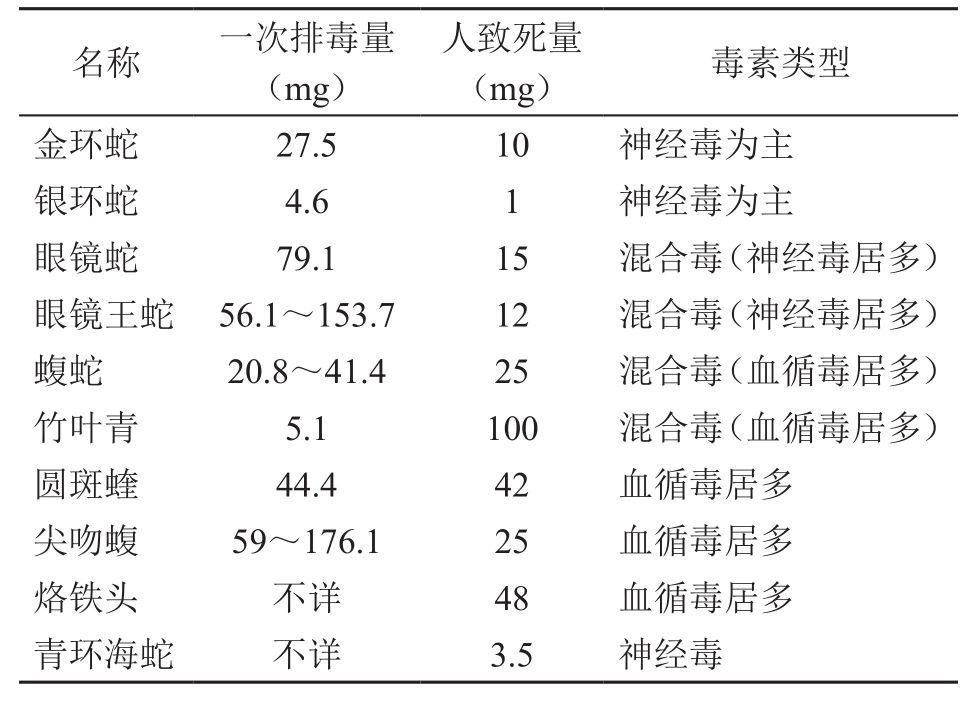
\includegraphics[width=3.25in,height=2.33333in]{./images/Image00229.jpg}
\end{table}

\subsection{诊断}

\subsubsection{临床表现特点}

\hypertarget{text00172.htmlux5cux23CHP5-8-1-2-1-1}{}
(一) 按毒蛇作用类别

\paragraph{神经毒素表现}

主要见于银环蛇、金环蛇和海蛇等咬伤。

\hypertarget{text00172.htmlux5cux23CHP5-8-1-2-1-1-1-1}{}
(1) 局部表现:

局部症状轻,仅有麻痒感。

\hypertarget{text00172.htmlux5cux23CHP5-8-1-2-1-1-1-2}{}
(2) 全身表现:

咬后1~4小时出现全身中毒症状。病情发展迅速,主要为横纹肌弛缓性瘫痪,首先出现视力模糊、眼睑下垂、声嘶、言语和吞咽困难、共济失调、牙关紧闭,继而向肢体发展,侵犯呼吸肌致呼吸肌麻痹,出现呼吸困难、呼吸衰竭,甚至惊厥、昏迷。

\paragraph{血循毒素表现}

主要见于蝰蛇、五步蛇、竹叶青蛇等咬伤。

\hypertarget{text00172.htmlux5cux23CHP5-8-1-2-1-1-2-1}{}
(1) 局部表现:

局部疼痛、肿胀,且向整个伤肢蔓延,伴有出血或局部组织坏死及局部淋巴结肿痛。

\hypertarget{text00172.htmlux5cux23CHP5-8-1-2-1-1-2-2}{}
(2) 全身表现:

发热、心悸、烦躁不安、谵妄、心律失常,可出现鼻出血、便血、呕血、咯血、血尿、皮肤黏膜出血点和瘀斑,重者颅内出血、少尿或无尿。由于出血和溶血反应致贫血、黄疸、血红蛋白尿,严重者发生循环衰竭和急性肾功能衰竭、甚至DIC。

\paragraph{混合毒素表现}

即可同时出现神经毒和血循毒的症状,主要见于眼镜蛇、眼镜王蛇、蝮蛇咬伤。

\hypertarget{text00172.htmlux5cux23CHP5-8-1-2-1-2}{}
(二) 按毒蛇种类不同,临床表现各异(表\ref{tab60-3})

\hypertarget{text00172.htmlux5cux23CHP5-8-1-2-1-3}{}
(三) 蛇毒中毒死亡原因

\paragraph{呼吸肌麻痹}

常见于银环蛇、金环蛇、海蛇蛇伤,也可见于眼镜蛇、眼镜王蛇毒中毒,若抢救不及时,发展为缺氧性脑病,窒息死亡。

\begin{table}[htbp]
\centering
\caption{10种常见毒蛇咬伤的临床表现}
\label{tab60-3}
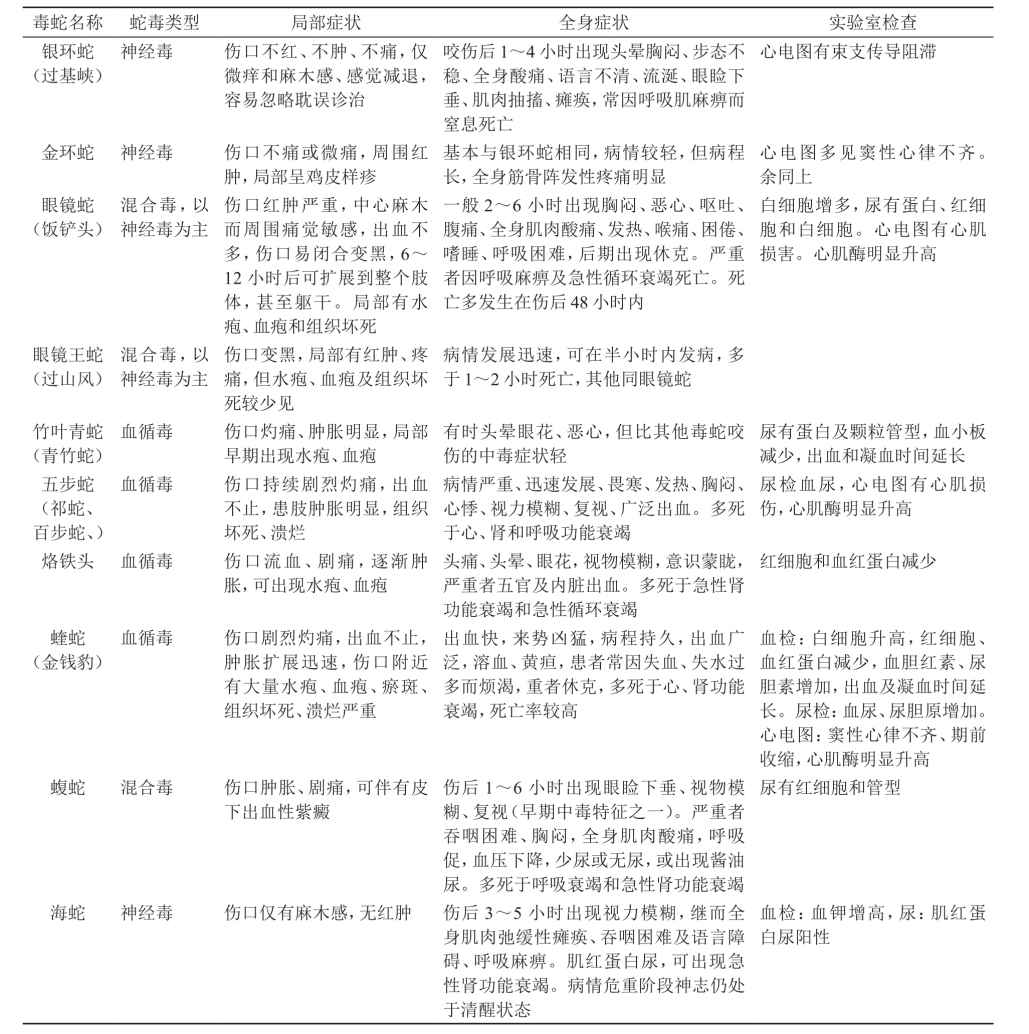
\includegraphics[width=6.83333in,height=6.86458in]{./images/Image00230.jpg}
\end{table}

\paragraph{循环衰竭}

常见于蝰蛇、五步蛇、烙铁头等毒蛇伤,因出凝血障碍所致,也可见于眼镜蛇、眼镜王蛇等蛇毒的心脏毒引起心力衰竭而造成。

\paragraph{急性肾功能衰竭}

常见于蝰蛇毒溶血产生的大量血红蛋白,其次是五步蛇、蝮蛇和海蛇毒损害骨骼肌所产生的大量肌红蛋白,在酸性尿中,沉积于肾小管,阻塞肾小管,引起急性肾功能衰竭。

\paragraph{出血及凝血障碍}

常见于蝰蛇、五步蛇伤,可出现广泛出血、溶血,严重者可导致脑出现而死亡。

\paragraph{感染}

创面坏死感染、气性坏疽、败血症及创口合并破伤风,呼吸麻痹后引起坠积性肺炎、吸入性肺炎、真菌感染等而致死。

\paragraph{其他}

严重中毒者,引起肾上腺皮质功能衰竭是蛇伤中毒死亡的辅因。

\subsubsection{实验室检查项目}

1.三大常规检查
①血常规:红细胞、白细胞计数和分类。此外,还应注意检查血小板的数量。合并贫血者应注意血红蛋白和血细胞比积、网织红细胞计数等检查。②尿常规:应注意有无血尿、蛋白尿、血红蛋白尿、管型等。应观察24小时尿量多少,对危重患者必须记录每小时尿量。③大便常规:对有出、凝血功能障碍的蛇伤者,应做大便潜血试验,了解是否存在消化道出血情况。

2.血生化检查
血电解质、血尿素氮、血肌酐、血气分析、心肌酶、肝功能、凝血功能、纤维蛋白原定量、3P试验,以了解肝、肾、心以及血液系统等功能。

3.心电图检查。

4.特殊试验
①乳胶抑制试验:应用蛇毒抗原抗体反应,可检测患者为何种毒蛇咬伤;出现凝集反应者为阴性,均匀混浊者为阳性,提示为该种毒蛇咬伤。②乳凝试验:测定患者血清中抗体,可推测为何种毒蛇咬伤。不凝者为阴性,凝集者为阳性。试验适用于晚期蛇咬伤的患者。

\subsubsection{诊断注意事项}

\paragraph{诊断问题}

①明确蛇咬伤史:局部有牙痕一对或伴有伤口肿痛、出血、渗血不止和全身症状则可拟诊毒蛇伤。②分辨何种毒蛇:可向患者或在场人员询问毒蛇形态,最好能捉住或打死毒蛇带到医院对照图谱识别。③根据伤者的局部及全身症状表现判断属何种或何类毒蛇伤,如神经毒、血循毒、混合毒毒蛇伤,病情严重程度如何。④记录被咬的时间、地点,并密切注意局部和全身症状的发展情况。

\paragraph{鉴别诊断问题}

主要应注意以下两点:①毒蛇伤与无毒蛇咬伤的鉴别(表\ref{tab60-4}):在通常情况下,毒蛇咬伤,病情较重,不但局部症状明显,而且很快出现全身中毒症状,治疗不及时或失当,可导致死亡。无毒蛇咬伤病情较轻,仅有轻微局部症状,无全身中毒症状表现,对生命没有危险。如不能肯定时,按毒蛇咬伤处理,严密观察。②有关可能导致误诊的问题:在临床中,可遇到个别人将某些毒虫(如蜈蚣、黄蜂)咬伤或荆棘刺伤皮肤误诊为毒蛇伤前来就诊,也有因某些神经毒素蛇咬伤(如银环蛇等),伤后无明显局部症状,全身中毒症状尚未出现时,因而容易为患者和医生所忽视而误作其他无毒蛇咬伤。若遇此情况,必须留患者临床观察。

\subsection{治疗}

\subsubsection{救治原则}

千方百计减少蛇毒的继续吸收、增加蛇毒的排泄,尽早足量使用相应的抗蛇毒血清,对症处理,保护脏器功能。

\subsubsection{现场伤口局部处理}

现场保持镇静。就地取材处理伤口,愈快愈好。①火柴烧灼法:用于银环蛇伤。其毒牙短,伤口浅,蛇毒仅在皮下。即点燃几根火柴,烧灼伤口(瞬间局部高温,蛇毒蛋白发生凝固,失去活性)。此法必须蛇伤后数分钟内及时处理。②结扎:在伤肢近心端扎紧,松紧程度以能阻断静脉及淋巴回流,但不妨碍动脉血流为宜,每20分钟放松1~2分钟,至伤口彻底处理后解除,一般不超过2小时为宜。③伤肢处理:搁伤口下垂位,静置、限制活动,伤口周围置冰袋冷敷减少蛇毒吸收。

\subsubsection{院内处理}

\hypertarget{text00172.htmlux5cux23CHP5-8-1-3-3-1}{}
(一) 程序化综合救治方法

\paragraph{切开冲洗、负压吸引排毒}

按毒蛇牙痕方向纵切开,如看不清牙痕,则作“十”字形切开0.5cm,深达真皮,使淋巴液外流,并用生理盐水或1/5000高锰酸钾液迅速充分冲洗,用大注射器或吸引管负压吸引,彻底排毒后敷盖消毒敷料,持续湿敷伤口以利排毒。注意伤口切开不要太长以免加快蛇毒吸收出现突然病情加重现象。

\paragraph{局部封闭疗法}

\begin{table}[htbp]
\centering
\caption{毒蛇与无毒蛇咬伤的鉴别}
\label{tab60-4}
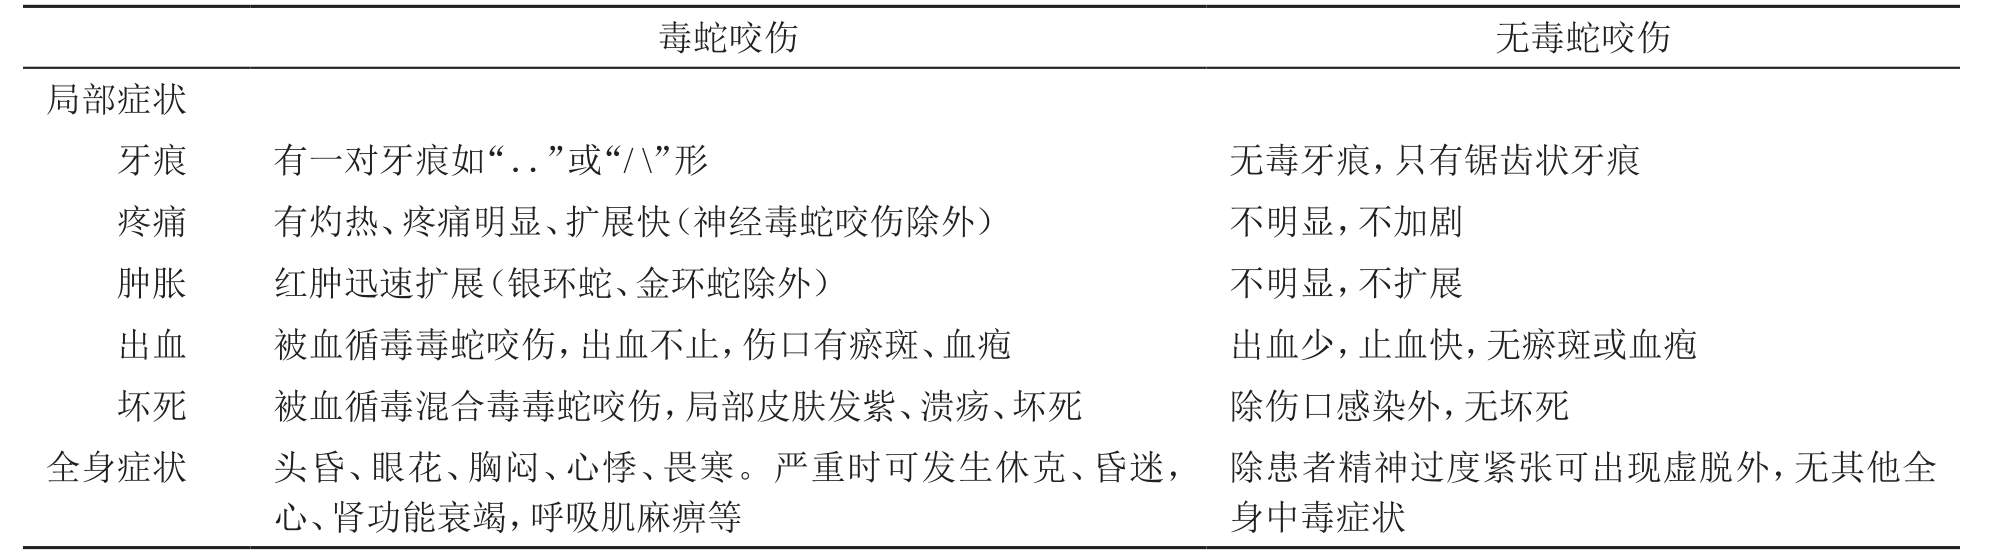
\includegraphics[width=6.69792in,height=1.85417in]{./images/Image00231.jpg}
\end{table}

利用同种或相应的抗蛇毒血清局部中和蛇毒的原理阻断蛇毒的继续吸收。用法:2\%利多卡因5ml加甲泼尼龙40mg(或地塞米松10mg)及同种抗蛇毒血清1/2支加入生理盐水10ml稀释,在伤口近心端上关节处行环形局部封闭,伤口离关节较远时可在伤口周围局部封闭,在伤口周围肿胀处加用20\%硫酸镁溶液湿敷。联合用药有止痛、消炎、减少组织对蛇毒的过敏反应并能中和蛇毒作用。还可以用以下其中之一方法处理:①胰蛋白酶:是一种强有力的蛋白水解酶------肽链内断酶。它能迅速中和蛇毒中的毒性蛋白,使蛇毒失去毒性。早期局部应用,对各种蛇伤均有效,尤其对银环蛇、眼镜蛇疗效显著。用法:胰蛋白酶结晶2~4mg,加入0.25\%~0.5\%普鲁卡因2~4ml溶液中,在伤口周围皮下浸润注射,并在伤口肿胀的上方,作环状封闭。②糜蛋白酶:其性能与胰蛋白酶基本相同,与蛇毒相遇后,即可产生水解作用,使蛇毒分解而失去毒性。但分解蛇毒作用不及胰蛋白酶强而有力。用法:糜蛋白酶5~10mg加入生理盐水5~10ml,在伤口周围和肿胀部位的上方作环状封闭。③依地酸钙钠:具有中和蛇毒及其有关脂酶(如PLA\textsubscript{2}
)的作用。用法:依地酸钙钠0.4g,加入0.25\%普鲁卡因溶液5~10ml作局部封闭,每日1次,连续2天。

\paragraph{尽早足量使用抗蛇毒血清}

抗蛇毒血清是国际公认的治疗蛇伤的特效药,采用抗蛇毒血清治疗已100多年,国内临床使用也已30多年。主要组成成分是经胃酶消化后的马蛇毒免疫球蛋白。抗蛇毒血清是通过抗原抗体中和反应而迅速出现疗效。当抗蛇毒血清注射入患者体内,起到中和蛇毒和破坏蛇毒的作用。及早使用抗蛇毒血清,可使患者不出现中毒症状,对已产生中毒症状者可控制病情发展。抗蛇毒血清对蛇毒已造成的脏器损害无直接保护作用。目前国内生产的抗蛇毒血清多为单价血清,分别是抗眼镜蛇毒血清(1000U/支)、抗银环蛇毒血清(10
000U/支)、抗蝮蛇毒血清(6000U/支)、抗五步蛇毒血清(2000U/支)、抗蝰蛇毒血清(5000U/支)。

\hypertarget{text00172.htmlux5cux23CHP5-8-1-3-3-1-3-1}{}
(1) 使用原则:

根据毒蛇咬伤的种类使用对应的抗蛇毒血清。如不明蛇种,可按有神经毒素表现加用抗银环蛇毒血清,有血循毒表现加用抗蝮蛇毒血清和(或)抗五步蛇毒血清,混合毒素表现则用抗银环蛇毒血清和抗蝮蛇毒血清{[}和(或)抗五步蛇毒血清{]}。对无特异性抗蛇毒血清的毒蛇伤,研究证明抗五步蛇毒血清和抗蝮蛇毒血清能中和烙铁头蛇毒或竹叶青蛇毒;抗眼镜蛇毒血清、抗银环蛇毒血清配伍能中和眼镜王蛇毒和泰国眼镜蛇毒。海蛇伤则用抗银环蛇毒血清、抗眼镜蛇毒血清及抗蝰蛇毒血清三种联用。

\hypertarget{text00172.htmlux5cux23CHP5-8-1-3-3-1-3-2}{}
(2) 应用时机:

根据抗蛇毒血清原理是中和未对靶器官起毒效应的游离蛇毒和结合后再次游离出血液的蛇毒,故其疗效完全取决于伤后投药时间,愈早愈好,力争在伤后2小时内用药效果最佳。一般伤后24小时内,抗蛇毒血清应列为常规用药。

\hypertarget{text00172.htmlux5cux23CHP5-8-1-3-3-1-3-3}{}
(3) 使用剂量:

在临床中,对抗蛇毒血清应用剂量,应根据临床症状,结合被蛇咬伤的时间来判断中毒程度决定注射抗蛇毒血清剂量。就诊早未出现全身症状者用抗蛇毒血清1~2支;如果伤后仅数小时,病情发展迅速,表明进入体内的蛇毒量较大,应加大抗蛇毒血清量2~4倍,加强观察,如症状渐加重1~2小时内追加1~2支。小孩与成人剂量相同,国产抗蛇毒血清比进口效果好。各种抗蛇毒血清治疗剂量参考表\ref{tab60-5}\footnote{上述剂量一般能中和一条相应毒蛇的排毒量,可以根据病情酌量增加用量}。

\begin{table}[htbp]
\centering
\caption{各种抗蛇毒血清治疗剂量}
\label{tab60-5}
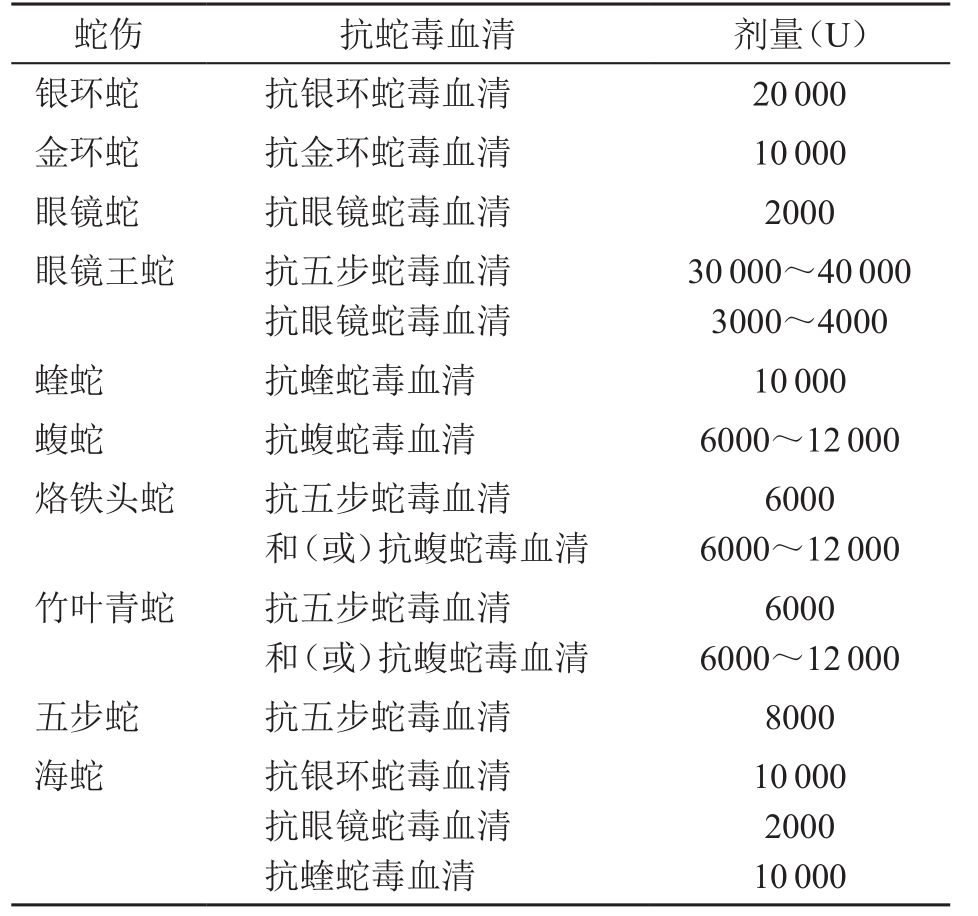
\includegraphics[width=3.25in,height=3.04167in]{./images/Image00232.jpg}
\end{table}

\hypertarget{text00172.htmlux5cux23CHP5-8-1-3-3-1-3-4}{}
(4) 用法:

开放2条静脉通道,抗过敏和抗蛇毒血清治疗同时进行。1条先静滴甲泼尼龙125~250mg(无甲泼尼龙时用地塞米松10~20mg代替);另1条静滴抗蛇毒血清,同时肌注苯海拉明20mg。

“分段稀释静脉滴注法”:为争取治疗时间,把皮试、脱敏、治疗叠合为一。方法:抗蛇毒血清1~2支(安瓿)加入5\%葡萄糖注射液250ml,先以30ml/h的速度静脉滴注,30分钟后若无过敏反应,则其余2小时内滴注完。在抗蛇毒血清治疗期间应密切观察治疗反应。

\paragraph{用抗蛇毒血清出现严重不良反应的处理}

①过敏性休克:可在注射中或注射后数分钟至数十分钟内突然发生。表现为突然沉郁或烦躁、脸色苍白或潮红、胸闷或气喘、出冷汗、恶心或腹痛、脉搏细速、血压下降、重者昏迷虚脱。抢救:马上停用抗蛇毒血清,保留静脉通道,吸氧,皮下注射肾上腺素、并使用抗过敏药物和肾上腺皮质激素,必要时加升压药。②血清病:一般出现在注射后7~14天(延缓型),也可在注射后2~4天内(加速型)发生。表现为荨麻疹、发热、淋巴结肿大、局部水肿,偶有蛋白尿、呕吐、关节痛,注射部位出现红斑、瘙痒及水肿。处理:使用钙剂或抗组织胺药物。一般数日至十数日可痊愈。

\hypertarget{text00172.htmlux5cux23CHP5-8-1-3-3-2}{}
(二) 争分夺秒抢救威胁生命的毒效应危象 ,保护脏器功能

对出现呼吸衰竭、急性肾功能衰竭、DIC等即置于急诊ICU进行专门抢救(如气管插管、机械通气、血液净化等)。

蛇毒所致的毒效应危象包括呼吸衰竭、心搏骤停、休克、肺水肿、DIC及急性肾功能衰竭等。如患者被神经毒毒蛇咬伤后,一旦出现呼吸困难,很快便进入呼吸肌麻痹而呼吸停止,故必须在此之前行气管插管术以机械通气支持呼吸,避免因机体严重缺氧而导致像多米诺骨牌样反应出现多脏器功能衰竭或因心肌缺氧导致心搏骤停,同时注意防止坠积性肺炎和吸入性肺炎,勤翻身拍背,必要时可用纤维支气管镜直视下吸痰。

血液净化如血浆置换、血液灌流等对于危重型毒蛇伤是当前有效的抢救手段。

\hypertarget{text00172.htmlux5cux23CHP5-8-1-3-3-3}{}
(三) 加强监测,防治可能发生的并发症

对不同种类的蛇伤监测内容可有所侧重。神经毒毒蛇伤监测重点是呼吸频率、节律、血氧饱和度及血气分析等;血循毒毒蛇伤重点监测血常规、尿常规、每小时尿量,血小板计数、凝血酶原时间、纤维蛋白原定量、3P试验、心肌酶、肝功能、血肌酐、血尿素氮等。

1.呼吸监测 如呼吸肌麻痹出现呼吸衰竭,立即行气管插管术机械通气支持呼吸。

2.监测血压 ,及时补足血容量
酌情使用血浆、代血浆,保证尿量100ml/h,以利排毒。若出现休克,可考虑深静脉置管监测CVP指导输液;纠正酸中毒,必要时给予强心药。血容量补足后仍尿少可使用呋塞米(速尿)等利尿剂。

3.监测尿常规
包括每小时尿量、尿比重,同时监测血肌酐、血尿素氮,如出现急性肾功能衰竭表现,有以下情况应及早采用替代疗法即血液透析治疗:①连续2天少尿或无尿。②尿毒症症状。③肌酐清除率较正常下降超过50\%,或在原肾功能不全基础上,肌酐清除率又下降超过15\%;或血肌酐>
442μmol/L,血尿素氮> 21mmol/L。④肌酐每天升高>
100μmol/L。如合并凝血功能障碍,可用无肝素透析疗法,每2天1次,至肾功能恢复好转。

4.监测心电、心肌酶
发现致命性心律失常及泵衰竭应及时给予对应处理,并可使用心肌营养剂。

5.监测血液功能 ,早期防治DIC
常规用每天低分子右旋糖酐500~1000ml,双嘧达莫(潘生丁)200~400mg;丹参20~40ml,疗程5~7天。必要时补充血小板、纤维蛋白原等。严重贫血者可给予输血,力求输入新鲜血以能补充凝血因子。

6.糖皮质激素应用
可提高机体对蛇毒的应激,对出血、溶血、细胞坏死有一定的治疗作用。用法:大剂量、短疗程,常用地塞米松20mg加入补液中静滴,每天2次,或甲泼尼龙125~250mg/次静注或静滴,每天2次,一般不超过3天。

\hypertarget{text00172.htmlux5cux23CHP5-8-1-3-3-4}{}
(四) 常规治疗

1.选用合理抗生素控制感染。

2.注射破伤风抗毒素(TAT)(皮试)1500~3000IU预防破伤风。

3.输液疗法维持水
、电解质平衡,保持热量。病情超过3天的危重患者要考虑给予营养支持。

\hypertarget{text00172.htmlux5cux23CHP5-8-1-3-3-5}{}
(五) 中草药治疗

(可根据当地药源灵活运用)

\hypertarget{text00172.htmlux5cux23CHP5-8-1-3-3-6}{}
(六) 外科治疗

蛇伤患肢肿胀明显可考虑切开引流减压
,坏死组织必须及早清除,以免增加毒素吸收,促发多脏器功能衰竭。对于伤口溃烂(主要见于眼镜蛇伤),可通过整形技术治疗。

\subsubsection{毒蛇伤特殊情况治疗}

1.“假性脑死亡”见于神经毒或以神经毒为主的混合毒类毒蛇伤,患者出现深昏迷、脑干反射消失,眼球固定、双瞳孔散大、对光反射消失、无自主呼吸、需用升压药维持,仅有心跳,容易被误认为是脑死亡而放弃抢救,但经积极治疗可痊愈,因此被称为神经毒素所致的“假性脑死亡”。救治:气管插管,呼吸机维持通气。尽早用血液净化技术如血浆置换、血液灌流等将蛇毒排出体外,在准备血液净化器械前先按程序化使用1支抗银环蛇毒血清以中和体内蛇毒,血液净化后再加用2支抗银环蛇毒血清。部分蛇毒与组织受体结合力强不易分离或分离慢,必要时第二天再重复1次,至患者清醒止。

2.眼镜王蛇咬伤
部分地区死亡率高达80\%。救治:早期足量使用抗眼镜蛇毒血清和抗银环蛇毒血清,同时尽早用血液净化治疗,出现呼吸衰竭用呼吸机人工通气。

3.眼镜蛇咬伤
眼镜蛇毒液主要毒性成分包括细胞毒素、神经毒素及一些酶类,其毒性蛋白可引起咬伤部位疼痛、红肿、渗出及疏松结缔组织水肿与坏死,临床上尤以细胞毒素表现最为突出。在正常情况下,人体血管能通过的相对分子质量约为5000,而中华眼镜蛇毒的相对分子质量为11
100,一般不易进入血管。中华眼镜蛇细胞毒素主要沿着肌间隙、淋巴管渗透,容易聚积在疏松结缔组织较多的部位如手背或足背处,被其毒素侵入的细胞很快就发生胞膜破裂、核溶解,组织结构模糊不清等坏死性改变,在坏死区周围可见组织细胞严重肿胀、空泡变性及微血管栓塞等损伤性改变。有些受伤肢体局部组织由于蛇毒的作用使血管神经受损,血液循环障碍而致溃疡迁移不愈,随着时间发展为坏死不断扩大从而导致局部皮肤软组织肿胀坏死广泛,最终必须进行植皮甚至截肢治疗。所以对于眼镜蛇咬伤患者,一定要对伤口清创彻底,防止进一步破坏,同时要注意向心性潜行破坏到其他地方,引起其他地方溃烂坏死。

4.竹叶青蛇伤
可引起血液功能障碍,出现类DIC的血液改变,如血小板、血浆纤维蛋白原含量减少、3P试验阳性、PT异常等,但临床表现较轻,仅出现皮下出血、血尿等,不出现诸如休克、多发性微血管栓塞等症状。甚至会在病后3~7天时出现症状缓解而血液检查加重的症状与血液检查分离现象。治疗:一般按常规治疗加连用3天皮质激素如甲泼尼龙125mg,每天3次,严重者可加用新鲜冰冻血浆400ml或血小板1~2单位。

5.危重型毒蛇伤
主要出现在血循毒的毒蛇伤,如蝰蛇咬伤,病情变化复杂,容易出现多脏器功能损害,一般早期表现有血浆渗漏到第三间隙的“渗漏综合征”,全身水肿、血容量不足,低钠血症等。救治:综合救治措施,足量应用抗蛇毒血清;低分子右旋糖酐500ml
+ 654-2 20mg
+丹参注射液16ml静滴,每天1次,连用1周;甲泼尼龙125mg静注,6小时一次,连用3天;羟乙基淀粉(霍姆)250ml/d静滴,连用3天。必要时加用血液净化如血浆置换或无肝素血液透析。

6.DIC治疗
常见于血循毒蛇伤,表现为出血、溶血和急性肾功能衰竭,容易诱发多脏器功能衰竭甚至导致死亡,主要以预防为主。救治:根据病情输血小板、冷凝集或纤维蛋白原,补充凝血因子,最好输新鲜血浆或全血。必要时采用无肝素血液透析。抗凝治疗是阻断DIC病理过程最主要的措施之一,由于蛇毒的促凝作用,一般不能被肝素所拮抗,所以不使用肝素抗凝。

7.“无毒”蛇或游蛇类咬伤后出现中毒表现
某些蛇(主要是游蛇类),易被认为是无毒蛇作为宠物蛇家养,不小心咬伤后出现中毒表现,其处理流程是伤口常规处理后,针对中毒表现分辨出血循毒抑或是神经毒,选用抗神经毒或血循毒的抗蛇毒血清。

8.孕妇毒蛇伤
蛇毒主要有神经毒、血循毒和混合毒,毒作用复杂、严重,易引起孕妇出血、溶血、休克、DIC等,以及其并发症可引起胎盘早剥、胎儿宫内窘迫等,导致流产、早产、死胎。孕妇与胎儿之间存在胎盘屏障,大分子除免疫球蛋白G以外,其他蛋白质之类的物质均不能直接通过胎盘进入胎体。经纯化处理后的精制抗蛇毒血清制品主要成分F(ab),该成分不能通过胎盘进入胎体。因此,关键是要尽早使用足量的精制抗蛇毒血清,及时中和体内的蛇毒素,才能对孕妇和胎儿起到保护作用。

9.患肢肿胀
在伤口周围肿胀处用20\%硫酸镁溶液湿敷,可加用多磺酸粘多糖乳膏(喜疗妥)涂在患肢肿胀部位,必要时可在湿敷的基础上加用红外线照射15分钟,每6小时1次;也可用针刺减压。

10.缺乏单价抗蛇毒血清地区
,在严格按流程处理伤口的基础上,可尝试用冻干多价抗蛇毒血清,或根据病情采用血液净化。

11.毒蛇伤治愈后
,患肢1~3个月后再次肿胀,原因未明,可能与毒素引起的迟发性反应有关。治疗:用20\%硫酸镁湿敷患肢,红外线灯照射15分钟,每天6次。

关于预后问题,据文献报道,没有蛇伤特效药之前,有些地区蛇伤年平均病死率为4\%。自20世纪70年代有了特效药------抗蛇毒血清以来,蛇伤年平均病死率下降到0.4\%。一旦毒蛇伤后超过24~48小时未能得到抗蛇毒血清或血液净化治疗,如出现DIC或多脏器功能衰竭者预后不佳。

\subsection{预防}

蛇咬伤严重威胁着广大劳动者的身体健康,应在危害最大的地区,采取积极的预防措施,尽量减少蛇咬伤的发病率,降低死亡率。首先要建立健全的蛇伤防治网络,从组织上及人力上予以落实,做到任务明确,专人负责。其次要发动群众搞好住宅周围的环境卫生,彻底铲除杂草,清理乱石,堵塞洞穴,消灭毒蛇的隐蔽场所。普及预防蛇伤的基本知识。在野外从事劳动生产人员,进入草丛前,应先用棍棒驱赶毒蛇,在深山丛林中作业与执勤时,要随时注意观察周围情况,及时排除隐患,应穿好长袖上衣,长裤及鞋袜,必要时戴好草帽。驻地周围可撒少许硫黄用于驱蛇用。遇到毒蛇时不要惊慌失措,应采用左、右拐弯的走动来躲避追赶的毒蛇,或站在原处,面向毒蛇,注意来势左右避开,寻找机会拾起树枝自卫。

\hypertarget{text00172.htmlux5cux23CHP5-8-1-5}{}
参 考 文 献

1. 蓝海,陈远聪.中国毒蛇及蛇伤救治.上海:上海科学技术出版社,2008

2. 王舒茵
,梁子敬.红脖颈槽蛇咬伤1例并文献复习.中国急救医学,2009,29(12):1147-1148

3. 王蔚
,顾江红.妊娠期毒蛇咬伤6例临床分析.浙江中医药大学学报,2010,34(2)

\protect\hypertarget{text00173.html}{}{}

\section{河豚毒素中毒}

河豚毒素中毒(fugu
poisoning)是指进食带有河豚毒素(tetrodotoxin,TIX)的河豚而引起的中毒。

\subsection{病因与发病机制}

河豚分布于我国沿海和长江下游。TIX主要有河豚毒和河豚酸两种,它们主要存在于河豚的睾丸、卵巢、卵、肝、肠等组织和血液中。有些河豚的肌肉也有剧毒,如双斑园豚;暗色东方豚的肾脏亦含有剧毒。此两种河豚主要分布于长江下游,应予以重视。TIX毒性稳定,经炒煮、盐腌和日晒等均不能被破坏,它属于已知的小分子量、非蛋白质的神经性毒素,具有箭毒样毒作用,其毒性较剧毒的氰化钠还要大1000多倍,致死量约等于7μg/kg体重。常因误食或烹饪不当食后发生中毒。

TIX食入后,极易从胃肠道吸收,并迅速以原形自肾排出体外。TIX吸收后迅速地作用于神经末梢和神经中枢,通过与Na\textsuperscript{+}
通道受体结合,阻断电压依赖性钠通道,从而阻滞动作电位,导致与之相关的生理活动障碍,主要是神经肌肉麻痹。TIX作用于脑干、运动神经、感觉神经和自主神经系统,引起中枢神经、肌肉神经、心血管和胃肠道功能障碍等临床表现。先引起感觉神经麻痹,后致运动神经麻痹,呼吸肌麻痹,最终导致周围性呼吸衰竭。严重者出现脑干麻痹,导致中枢性呼吸、循环衰竭而死亡。此外,尚可阻断心脏的快钠通道,使细胞失去兴奋性并导致心律失常。对胃肠道有局部刺激作用。

\subsection{诊断}

河豚毒素中毒一般在进食后0.5~3小时内迅速发病,病情进展迅速,死亡病例的病程一般多在发病后4~6小时。首先出现上腹部不适,恶心、呕吐、腹痛、腹泻,甚至便血等胃肠道症状;继之出现神经麻痹症状:口唇、舌尖及肢端麻木,甚至全身麻木,全身乏力,随后出现共济失调、眼睑下垂、肌肉软瘫、呼吸困难、心律失常,心电图可出现不同程度的房室传导阻滞。严重病例呼吸表浅不规则、言语不清、昏睡、昏迷,最后呼吸中枢麻痹和血管运动中枢麻痹而死亡。

\subsection{治疗}

河豚毒素中毒无特效解毒剂。河豚毒素在人体内解毒和排泄较快,若发病后8小时未死亡者,多能恢复。因此,一旦发生中毒,应尽快给予各种排毒和对症处理措施,让患者渡过危急期:①立即予以催吐、洗胃、灌服活性炭、导泻,因河豚毒素在碱性溶液中不稳定,故洗胃液以2\%碳酸氢钠液为好。切勿因食入时间较长而放弃洗胃。必要时用盐水或肥皂水进行高位灌肠。②静脉输液,维持水、电解质平衡,促进毒素排泄,可用高渗葡萄糖液、甘露醇、呋塞米等;③肌肉麻痹者,可用马钱子碱2mg肌肉注射或皮下注射,同时用维生素B\textsubscript{1}
、B\textsubscript{12}
肌肉注射;④尽早应用大剂量肾上腺皮质激素;⑤呼吸困难者吸氧,应用呼吸兴奋剂尼可刹米0.375g和(或)洛贝林3mg肌肉注射,呼吸肌麻痹用人工呼吸机;循环衰竭者应注意抗休克、纠正心律失常;⑥抗胆碱药物有一定对抗毒素对横纹肌的抑制作用,可选用阿托品1~2mg、或东莨菪碱0.3~0.6mg或山莨菪碱20~40mg肌注或稀释后静注,依病情需要可重复应用。⑦有报道乙酰半胱氨酸是有效解毒剂,可早期用50~100mg/d加入液体中静滴。⑧危重者可予以血液透析或血液灌流治疗。

\protect\hypertarget{text00174.html}{}{}

\section{雪卡毒素中毒}

雪卡毒素(ciguatoxin,CTX)是由某些海藻产生的一种海洋毒素,由小鱼吃下带有毒素的海藻,毒素通过食物链富集积聚在较大的海鱼身上,人类食用了被毒化的海鱼,即引起中毒。毒藻多生活在珊瑚礁周围,因此带雪卡毒素的鱼种主要有珊瑚鱼(coral
fish)类(指生活在热带、亚热带海域的珊瑚礁周围和近海海岸的鱼类如西星斑、老虎斑、杉斑、苏眉等石斑鱼和鲈鱼),所以CTX中毒一般指食用有毒珊瑚鱼而引起的中毒。CTX是一种神经毒素,它能兴奋中枢及周围神经节胆碱受体。

\subsection{诊断}

\paragraph{病史}

有食用珊瑚鱼史。

\paragraph{临床表现特点}

常在吃鱼后1~6小时发生。主要表现有:①消化系统症状:恶心、呕吐、腹痛、腹泻,部分患者口中有金属味。②神经系统症状:口唇、舌、咽喉发麻或有针扎感;身体感觉异常:瘙痒或有蚁爬感;特异性的温度感觉倒错:手触热物有冷感,放入水中则有热感或“电击样”感觉;膝关节酸痛,下肢肌肉酸麻无力;抽搐,动作失调;部分出现听觉、视觉异常。③心血管系统症状:心悸、胸闷、头晕、乏力、出汗,甚则晕厥。

\subsection{治疗}

在吃下有毒的珊瑚鱼后4小时内应催吐、洗胃、导泻。静脉输液,纠正水电解质和酸碱平衡紊乱。阿托品可用于重症心动过缓。使用肾上腺皮质激素。在急性期静滴20\%甘露醇(1mg/kg),能缓解神经系统症状。其他对症处理包括:腹痛者给予阿托品解痉,皮肤瘙痒者用抗组胺药、葡萄糖酸钙注射液,肌肉、关节酸痛给予镇痛剂,焦虑不安给予抗忧郁药。

\protect\hypertarget{text00175.html}{}{}

\section{贝类中毒}

贝类中毒是指进食被毒化的贝类而引起的中毒。贝类(shellfish)属软体动物,种类甚多,常见引起中毒者有蛤贝(clam)、扇贝(pectinidae)、牡蛎(oysters)、贻贝(mussels)、蛤仔(venerupis)等。尚有一些螺类如泥螺、香螺、东风螺、织纹螺等也可发生此类中毒。可食贝类受毒化的原因与“赤潮”有关,在发生赤潮的海域,贝类摄食有毒的藻类,引起藻类毒素的蓄积,人食用此等贝类后即可发生中毒。其毒素(石房蛤毒素和贝毒素)可致神经肌肉麻痹和肝损害,部分可引起日光性皮炎。

\subsection{诊断}

\paragraph{病史}

有误食被毒化的贝类及螺类史。大多数患者发生在5~10月间。

\paragraph{临床表现特点}

不同毒贝含有的毒素不同,中毒表现也各异,一般有以下几种类型:①神经型:亦称麻痹性贝类中毒。引起此类中毒者主要为石房蛤毒素(saxitoxin,STX)所致。含此毒素贝类有扇贝、贻贝、蛤仔、织纹螺、香螺、东风螺等。潜伏期一般为0.5~3小时。早期有唇、舌、手指麻木感,进而四肢末端和颈部麻痹,直至运动麻痹、步态不稳,并伴有发音障碍、流涎、头痛、口渴、恶心、呕吐等,严重者因呼吸麻痹而死亡。②肝损害型:引起此类中毒有蛤仔、巨牡蛎,含毒成分为贝毒素(venerupin)。潜伏期一般为12~42小时,有长达7天者。初期有胃部不适、恶心呕吐、腹痛、疲倦,亦可有微热,类似轻度感冒。接着出现粟粒大小出血斑,齿龈出血。重者可有呕血、阴道出血、意识障碍或昏睡状态,预后不良。③日光性皮炎型:主要为泥螺所致。潜伏期一般为1~14天,多数在3天内发病。初起面部和四肢的暴露部位出现红肿,并有灼热、疼痛、发痒、发胀、麻木等感觉。后期可出现瘀血斑、水疱或血疱,破溃后引起感染。可伴有发热、头痛、食欲不振。轻者1周渐愈,重者可迁延数月。④胃肠炎型:潜伏期为10~12小时,有恶心、呕吐、腹泻、下腹痛等征象,属自限性。

\subsection{治疗}

\paragraph{催吐 、洗胃}

洗胃液可用1∶5000高锰酸钾液或生理盐水,或2\%碳酸氢钠液。活性炭50~100g灌服。

\paragraph{胃肠炎型和肝损害型}

补液利尿,加速毒素排出,同时用保肝等对症治疗。

\paragraph{神经型}

应用抗胆碱药物如阿托品、东莨菪碱等。其他治疗包括应用肾上腺皮质激素,如地塞米松等;呼吸麻痹者,气管插管接呼吸机;全身支持和对症治疗。

\protect\hypertarget{text00176.html}{}{}

\section{含高组胺鱼类中毒}

含高组胺鱼类(hyperhistamine
fishes)中毒是由于食用含有一定数量组胺的某些鱼类而引起的类过敏性食物中毒。引起此种食物中毒的鱼类主要是海产鱼中的青皮红肉鱼类(如鲐鱼、金枪鱼、沙丁鱼、秋刀、鳞鱼等)及淡水中养殖的鲤鱼,因污染于鱼体的细菌对组氨酸的分解作用,产生大量组胺,通过食用进入人体后引起毛细血管扩张和支气管收缩,导致一系列的临床症状。腌制咸鱼时,如鱼不新鲜或未腌透,鱼中含组胺较多,亦可导致中毒。

\subsection{诊断}

\paragraph{病史}

有食用不新鲜或腐败的海产青皮红肉鱼类或河产鲤鱼史。

\paragraph{临床表现特点}

潜伏期5分钟~1小时,多数为0.5~1小时。中毒患者呈现组胺反应:如脸红、头晕、头痛、心悸、胸闷和呼吸急促,眼结合膜充血、视物模糊、脸胀唇肿、口、舌及四肢发麻,恶心、呕吐、腹痛、全身潮红、瘙痒、呈现荨麻疹。重症患者可发生喉头水肿、过敏性休克等。症状轻者多于数小时内减轻,12小时内消失;重症可致死亡。

\subsection{治疗}

1.催吐、洗胃、导泻以排除毒物。静脉输液、利尿,促进毒物排泄。

2.抗过敏治疗
可选用赛庚啶(2~4mg/次,每日3次口服)、异丙嗪(25mg/次,肌注)、苯海拉明(20mg/次,肌注)及钙剂等,西咪替丁、雷尼替丁效果也较好。

3.症状严重者可予肾上腺皮质激素 。发生休克者按过敏性休克治疗。

\protect\hypertarget{text00177.html}{}{}

\section{鱼胆中毒}

鱼胆中毒(fish bile
poisoning)是指进食鱼胆而引起的中毒。导致鱼胆中毒者大多是淡水养殖的鱼类,如青鱼、鲢鱼、鲤鱼、鲩鱼、鲮鱼、鳙鱼等。鱼胆汁中含有一种具有极强毒性的蛋白质分解产物,即胆汁毒素(icthyogalltoxin),不易被乙醇和热破坏;鲜鱼胆汁中含有胆酸、水溶性鲤醇硫酸酯钠,后者抑制细胞色素氧化酶,影响细胞呼吸链导致细胞呼吸停止;使钙内流,溶酶体膜稳定性降低,造成细胞损伤。鱼胆汁中尚有多种过敏物质,如氰氢酸、组胺等。实验研究提示自身氧化性细胞损害可能是鱼胆中毒致多脏器损伤发生的机制之一。肾为主要排泄器官,临床中毒以肾损害为主。临床上以消化道症状、肾、肝功能损害为主要表现,部分患者出现血液系统及神经系统症状。

\subsection{诊断}

\paragraph{病史}

近期进食鱼胆史。

\paragraph{临床表现特点}

潜伏期15分钟~14小时,多数为0.5~3小时。①消化系统症状:中毒早期主要出现胃肠道症状如恶心呕吐、腹痛、腹泻等,严重者呕吐咖啡色液体,排酱油色稀水便。病后2~8天有肝损害征象,如肝大、肝区胀痛、黄疸、肝功能异常等,持续1~2个月。②肾功能损害症状:腰部酸胀疼痛、蛋白尿、血尿、少尿、无尿。急性肾衰竭是鱼胆中毒最致命的损害,常在发病后1~4天出现。③血液系统症状:部分严重者发生溶血,出现呕血、便血、鼻出血、球结膜及皮下出血。④中毒性心肌病:心动过速、心力衰竭等,并可发生阿-斯综合征。⑤神经系统症状:头晕、头痛、嗜睡、四肢远端及唇舌麻木、末梢感觉障碍。严重者出现谵妄、抽搐、昏迷等。

\subsection{治疗}

1.催吐、洗胃、导泻、灌服活性炭。吞服鱼胆后24小时来诊的患者,仍应洗胃。

2.肾上腺皮质激素
应早期应用皮质激素,以减轻肾小管对毒素的反应。地塞米松20~40mg/d或氢化可的松300~500mg/d加入液体中静滴。

3.血液净化疗法
防治急性肾衰竭是鱼胆中毒的救治重点。凡口服大剂量鱼胆中毒的患者,应考虑尽早行血液净化治疗。

4.对症支持治疗
包括补液,纠正水电解质和酸碱紊乱;利尿排毒;保护肝肾功能;溶血者用碳酸氢钠碱化尿液;防治脑水肿等。

\protect\hypertarget{text00178.html}{}{}

\section{其他动物性毒物中毒}

包括蝎子螫伤、蜂类螫伤、蜈蚣咬伤、毒蜘蛛螫伤、斑蝥中毒、蟾蜍中毒、动物肝及甲状腺中毒等,详见表\ref{tab60-6}。

\begin{longtable}{c}
 \caption{其他动物性毒物中毒}
 \label{tab60-6}
 \endfirsthead
 \caption[]{其他动物性毒物中毒}
 \endhead
 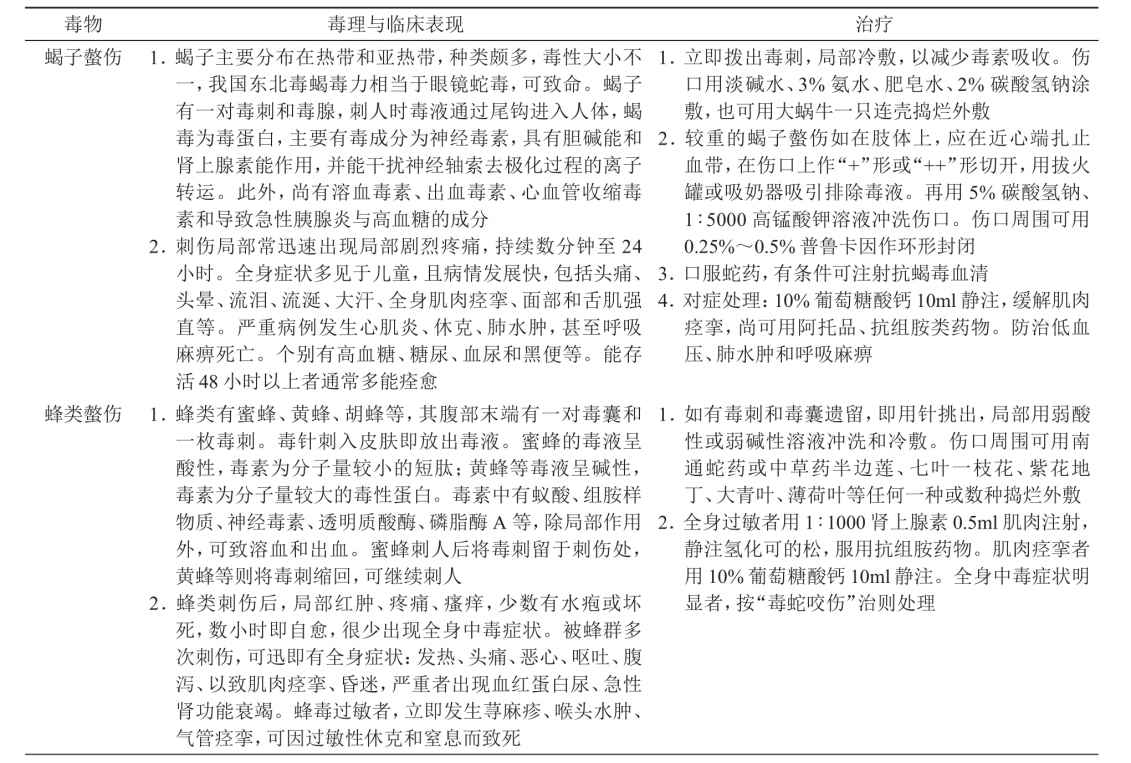
\includegraphics[width=\textwidth,height=\textheight,keepaspectratio]{./images/Image00233.jpg}\\
 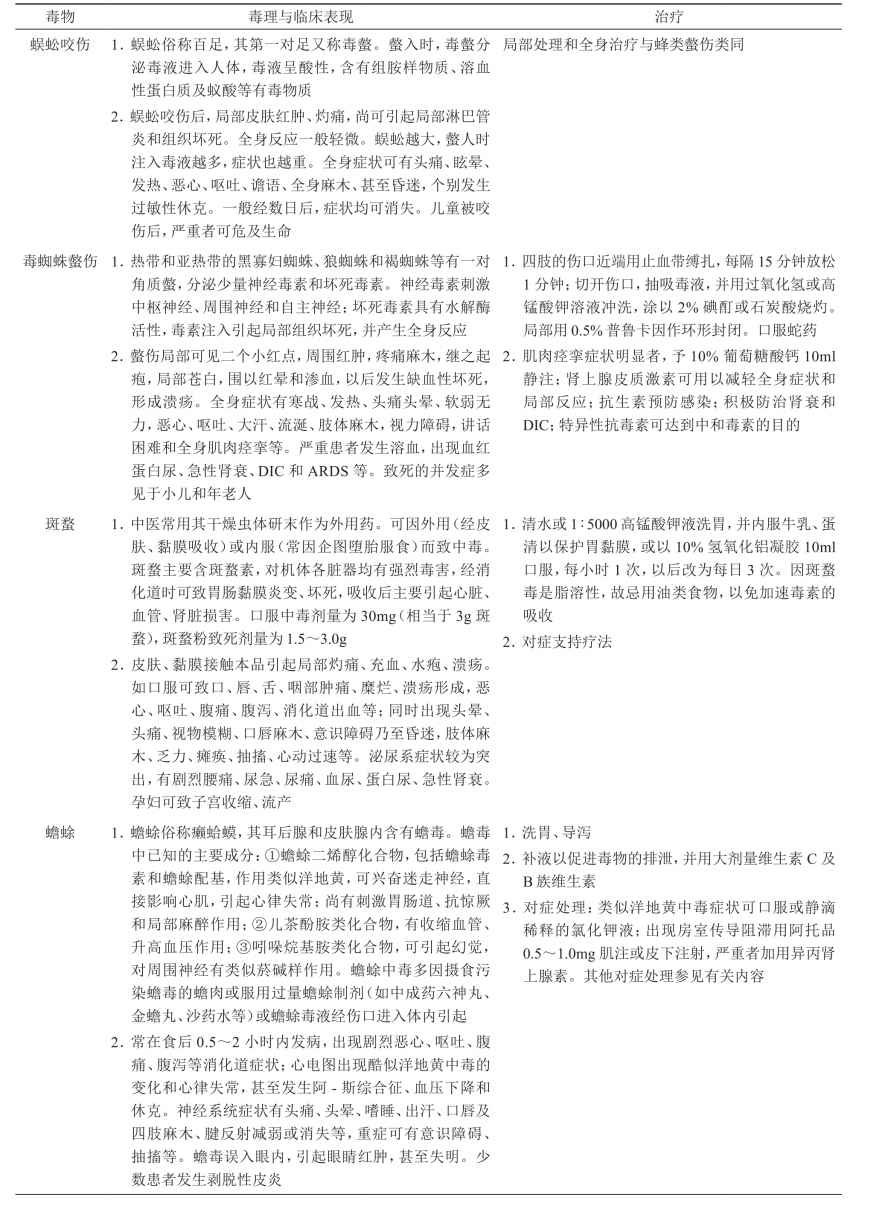
\includegraphics[width=\textwidth,height=\textheight,keepaspectratio]{./images/Image00234.jpg}\\
 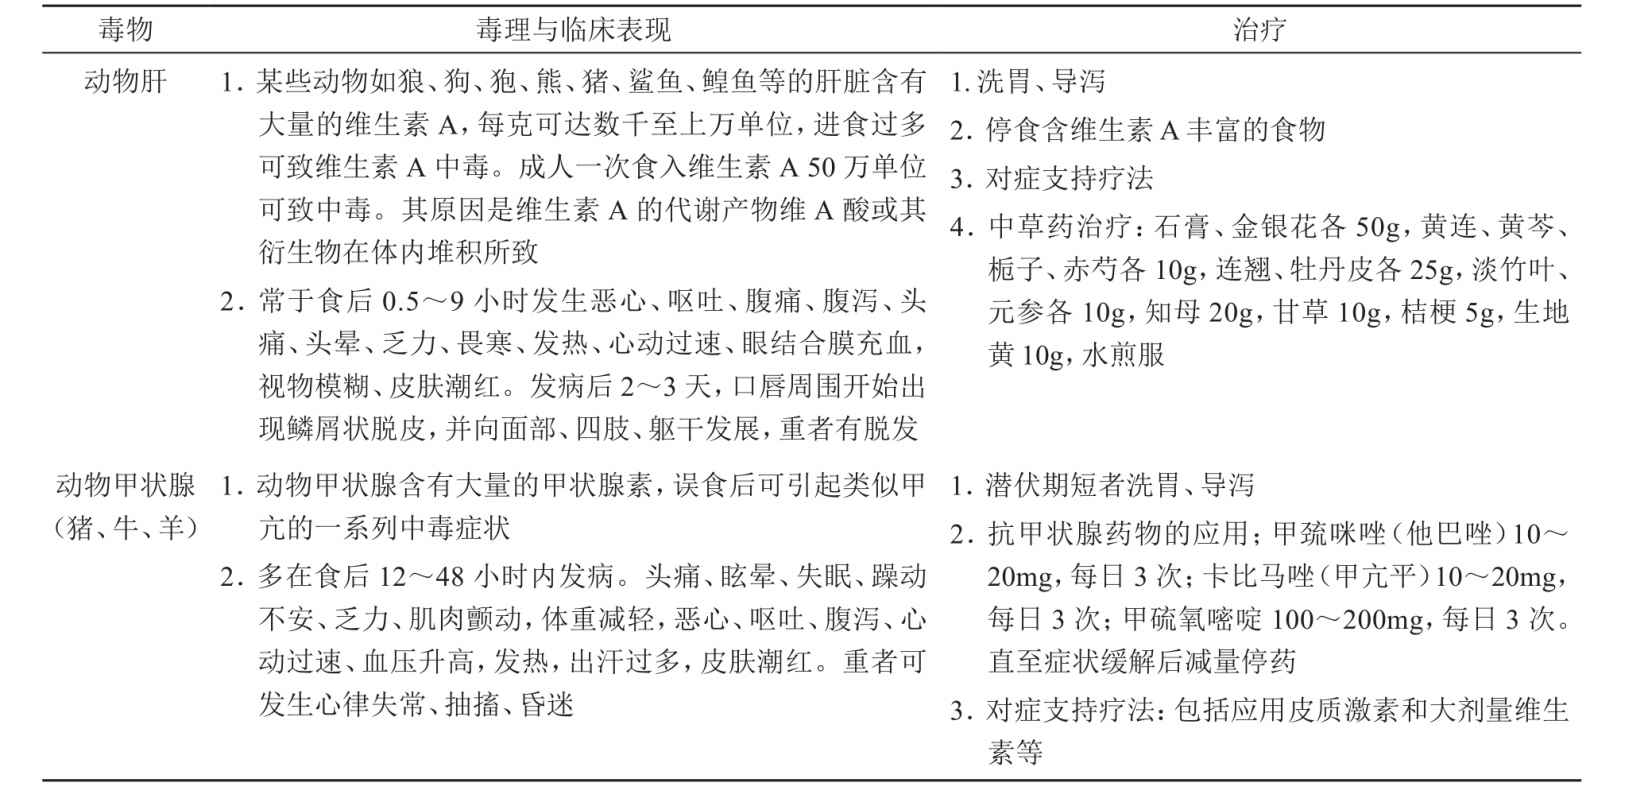
\includegraphics[width=\textwidth,height=\textheight,keepaspectratio]{./images/Image00235.jpg}
 \end{longtable}

\hypertarget{text00178.htmlux5cux23CHP5-8-7-1}{}
参 考 文 献

1. 张文武.急诊内科手册.北京:人民卫生出版社,2009

2. 朱子扬,龚兆庆,汪国良.中毒急救手册.上海:上海科学技术出版社,2007

3. 陈灏珠 ,林果为.实用内科学.第13版.北京:人民卫生出版社,2009

\protect\hypertarget{text00179.html}{}{}

\chapter{强酸强碱类中毒}

\section{强酸类中毒}

\subsection{病因与发病机制}

强酸(strong acids)主要指硫酸(sulfuric acid)、硝酸(nitric
acid)、盐酸(hydrochloric
acid)三种无机酸,均有强烈的刺激性和腐蚀性。此外氢氟酸(hydrofluoric
acid)及铬酸(chromium acid)毒性也强。浓有机酸如醋酸(acetic
acid)、甲酸(formic acid)、草酸(oxalic
acid)等的腐蚀作用较硫酸、硝酸为弱。中毒原因有经口误服,呼吸道吸入大量酸雾,皮肤接触而致腐蚀性灼伤。

强酸作用于人体组织使蛋白质凝固而发生凝固性坏死,组织细胞破坏,造成局部腐蚀性变化,表现为局部组织充血、水肿、坏死和溃疡,甚至腔管脏器穿孔,以后形成瘢痕、狭窄和变形。随着毒物吸收入血循环,引起内脏器官的损害,以肝、肾受损害较重。浓硫酸可放出三氧化硫,浓盐酸可放出氯化氢,浓硝酸可放出二氧化氮,经呼吸道吸入可致呼吸道腐蚀和灼伤,引起支气管炎、肺炎及肺水肿。强酸最小口服致死量,浓硫酸约为4ml,浓硝酸约8ml,浓盐酸约为15ml。铬酸的致死量约为6g。

\subsection{诊断}

\paragraph{病史}

有强酸接触史或误服史。

\paragraph{临床表现特点}

\hypertarget{text00179.htmlux5cux23CHP5-9-1-2-2-1}{}
(1) 局部表现:

①呼吸道化学性烧灼伤:见于吸入中毒。吸入强酸烟雾后立即出现呛咳、胸闷、呼吸困难、分泌物增多,咯泡沫样痰或咯血,听诊可有多量广泛的干湿性啰音。吸入量大者,有明显呼吸困难,发绀,喉头、气管、支气管痉挛、水肿,除加重呼吸困难外,甚至可导致急性窒息而死亡。由于强酸对肺泡的损伤,其通透性增加,渗出增多加之血液和淋巴液回流障碍,极易发生急性肺水肿。此外,眼亦会同时被强酸烟雾刺激而发生急性结膜、角膜或全眼炎,甚至招致失明。②皮肤化学性烧灼伤:见于接触性中毒。皮肤接触强酸后即发生灼伤、腐蚀、坏死和溃疡形成,其程度因接触的时间、面积和强酸液的数量而不同。因强酸与皮肤接触后引起细胞脱水,蛋白凝固,故灼伤后创面干燥,边缘分界清楚,肿胀较轻;不同种类的酸与皮肤蛋白形成不同的蛋白凝固物,故灼伤的痂皮或焦痂色泽,随酸的种类而异,如硝酸为黄色,硫酸为黑色或棕色,盐酸为灰棕色,氢氟酸为灰白色。以后瘢痕形成,甚至导致颜面、躯干或肢体的畸形和功能障碍。③消化道化学性烧灼伤:见于口服中毒。口服强酸后,口腔黏膜糜烂,可产生不同色泽痂皮。患者口、咽、喉头、食管、胃均有剧烈灼痛,恶心呕吐反复不已,呕吐物内含有血液和黏膜组织。食管及胃黏膜严重腐蚀,受损组织收缩变脆,严重时1~2天内可发生穿孔,继发弥漫性腹膜炎。虽有口渴,但因喉头水肿和痉挛,吞咽困难。急性中毒过后,常遗留食管瘢痕狭窄、幽门狭窄和消化道器质性或功能性紊乱等后遗症。草酸口服后引起低血钙,可致手足搐搦。

\hypertarget{text00179.htmlux5cux23CHP5-9-1-2-2-2}{}
(2) 全身性中毒表现:

主要有:①局部剧痛引起反射性精神神经症状或痛性休克。②大量强酸吸收入血,可致严重的酸中毒,肝、肾均呈明显损害征象,甚至发生急性肾功能衰竭。部分患者逐渐出现意识障碍,终至呼吸中枢麻痹而死亡。少部分患者可并有高铁血红蛋白血症。

氢氟酸中毒常可合并急性氟中毒,高渗性的氟离子可渗透组织深层,溶解细胞膜,造成表皮、真皮及皮下组织及肌层液性坏死,损害可深达骨膜,甚至骨骼无菌性坏死。氟离子与体内的钙、镁离子结合,形成不溶的氟化钙、氟化镁,出现低血钙、低血镁,可引起室性心律失常,甚至出现心搏骤停,心肌酶谱检查可明显升高。因设备意外及爆炸引起的氢氟酸外溢,可发生闪电样死亡。

\subsection{治疗}

\paragraph{吸入性中毒}

有喉头水肿、痉挛或窒息者,应及早施行气管切开术,并清除气管腔内的分泌物、脱落黏膜组织,确保呼吸道通畅和通气功能,并加压给氧或机械通气。可间断经气管导管滴入异丙肾上腺素、皮质激素、麻黄碱及普鲁卡因(做过敏试验)以减轻气管、肺对强酸刺激的炎症反应,松弛支气管平滑肌。有肺水肿或休克则予以相应处理。对于一般轻症病例可用2\%~4\%碳酸氢钠溶液雾化吸入。眼睛受到损害时,立即用大量清水或生理盐水彻底冲洗,然后给予可的松及抗生素眼药水交替滴眼,并密切观察,视情况作相应处理。

\paragraph{皮肤接触灼伤}

可立即用大量流动水冲洗,至少10分钟。然后局部用中和剂,如2\%~5\%碳酸氢钠、1\%氨水或肥皂水,以后再用水冲洗,以防酸进一步渗入。草酸及氢氟酸灼伤,局部及静脉注射10\%葡萄糖酸钙。

\paragraph{经口中毒}

一般禁忌催吐和胃管洗胃,以免加重食管和胃损伤或导致穿孔;也不能口服碳酸氢钠溶液,以免因产生CO\textsubscript{2}
气体而增加胃穿孔的危险。应即刻口服10\%氢氧化铝凝胶、2.5\%氧化镁溶液或7.5\%氢氧化镁混悬液60ml。内服润滑剂如生蛋清60ml调水或牛奶200ml,再服植物油100~200ml。立即补液,除5\%葡萄糖氯化钠溶液外,还应用碱性药物如5\%碳酸氢钠250~500ml或1.87\%乳酸钠500ml静滴以拮抗酸中毒。铬酸中毒用硫代硫酸钠静注,氢氟酸或草酸中毒用10\%葡萄糖酸钙10ml静注,并纠正电解质紊乱。为预防消化道瘢痕形成,在服酸后第2天起可给泼尼松口服每次10mg,每日3次,共2周。为预防食管狭窄应及早考虑扩张术。

\paragraph{对症支持疗法}

包括镇静止痛,补液,纠正酸中毒,防治休克,使用广谱抗生素预防感染,对重症患者加强对心肺和腹部情况的监护,及时发现和处理严重并发症。

\protect\hypertarget{text00180.html}{}{}

\section{强碱类中毒}

\subsection{病因与发病机制}

强碱类化学物中以氢氧化钠、氢氧化钾、氧化钠和氧化钾等腐蚀作用最强,其他如碳酸钠、碳酸钾、氢氧化钙和氢氧化铵,腐蚀作用较弱。中毒原因主要是经口误服,接触皮肤及眼部可发生灼伤。浓度极高的氢氧化铵也可严重损伤呼吸道器官。强碱类化学物能溶解组织蛋白和胶原组织,形成可溶性胶状碱性蛋白盐;与脂肪酸作用则皂化生成肥皂,导致组织坏死,结构破坏。由于组织易溶,碱类可深入组织深层,破坏易于扩散,故碱灼伤常较深。局部肿胀明显,丧失液量多,故碱灼伤患者成人总面积超过20\%、儿童超过10\%时要谨防因补液不足而发生休克。碱吸收后可引起碱中毒和肝、肾脂肪变性与坏死。其直接作用可引起皮肤黏膜溃烂、胃肠穿孔,并由此而导致一系列继发性病变。

\subsection{诊断}

\paragraph{病史}

有强碱类毒物接触史。

\paragraph{临床表现特点}

①皮肤黏膜接触强碱,可有局部灼痛、充血、水肿、糜烂或形成先为白色、后变为红棕色的痂,脱落后可形成溃疡。严重碱灼伤可引起体液丢失而发生休克。眼损害时可发生结膜炎、角膜炎、角膜溃疡。②吸入氢氧化铵释出的氨,有氨中毒表现和呼吸道刺激性症状。吸入高浓度氨气,少数因反射性声门痉挛而呼吸骤停。支气管损害严重,可咯出大量泡沫样痰及坏死组织,很快出现肺水肿,如不积极抢救,迅速发生休克和昏迷。③口服强碱后,口腔黏膜呈红色或棕色,有水肿、溃疡。口腔、咽喉、食管和胃有强烈烧灼痛,腹绞痛。反复呕吐,呕吐物中有血性液体,常有腹泻和血性大便。声音嘶哑、语言障碍和吞咽困难。严重病例可发生食管、胃穿孔。强碱吸收后可引起碱中毒和肝肾功能损害,出现手足搐搦。重症发生休克和昏迷,为早期死亡原因。后期可因继发感染、胃肠道出血及急性肾功能衰竭而危及生命。食管和胃黏膜病变较深,后遗狭窄很常见。

\subsection{治疗}

\paragraph{皮肤接触者}

要争取在现场立即用大量流动水冲洗,在清洗的同时即可清除腐皮,以防碱性物质继续皂化加深创面。冲洗时间至少20分钟,再用1\%醋酸冲洗创面。冲洗期间应不断用试纸测定创面的中和情况,直到创面的碱性逐渐减弱后停止冲洗。切勿在冲洗前应用弱酸中和剂,否则产生中和热量,加重灼伤。Ⅱ度以上灼伤用2\%醋酸溶液湿敷,眼灼伤时冲洗更应彻底,至少冲洗10~15分钟。石灰灼伤时,应先将石灰粉末拭干净,再用大量流水冲洗,以免石灰遇水生热,加重灼伤;禁用生理盐水冲洗,以免生成碱性更强的氢氧化钠。

\paragraph{口服中毒者}

应迅速应用弱酸溶液中和,如口服食用醋、1\%醋酸或5\%稀盐酸,但碳酸盐(如碳酸钠、碳酸钾)中毒时禁用,应改服硫酸镁,以免产生过多CO\textsubscript{2}
导致胃肠胀气、穿孔。接着给生蛋清及橄榄油。由于强碱作用迅速,不可拘泥于用上述灌胃液,最简便迅速的方法是立即口服1000~1500ml清水,稀释强碱的浓度。禁忌洗胃及导泻。支持疗法为补液纠正脱水,补充钙剂,防治休克及肾功能衰竭。当穿孔危险期过后,应尽早做食管扩张术。如吞咽困难发生较早,可先放置保留胃管,以阻止食管完全狭窄。早期应用1~2周的皮质激素,可减少食管瘢痕狭窄的发生。

\paragraph{吸入性中毒者}

吸氧,如发生急性肺水肿应及早做气管切开,因氨吸入后大量的呼吸道分泌物及脱落之假膜,可经气管切开处吸引管内吸出,以保持呼吸道通畅,预防窒息。早期施行雾化吸入,可减轻呼吸道灼伤程度。

\protect\hypertarget{text00181.html}{}{}

\hypertarget{text00181.htmlux5cux23CHP5-9-3}{}
参 考 文 献

1. Proudfoot AT. Acute Poisoning:Diagnosis and Management. 2nd ed.
Oxford:Butterworth Heinemann Ltd,1993

2. 陈灏珠 ,林果为.实用内科学.第13版.北京:人民卫生出版社,2009

\protect\hypertarget{text00182.html}{}{}

\chapter{食 物 中 毒}

\section{食物中毒诊断标准及技术处理总则}

\subsubsection{食物中毒与食源性疾病}

食物中毒(food
poisoning)是最常见的突发公共卫生事件之一。我国法定的食物中毒定义有两个:一个是中华人民共和国国家标准《食物中毒诊断标准及技术处理总则》(GB14938---94,1994年8月1日起实施)将食物中毒定义为:“摄入了含有生物性、化学性有毒有害物质的食品或者把有毒有害物质当作食品摄入后出现的非传染性(不属于传染性)的急性、亚急性疾病。”另一个是2000年1月1日起施行的卫生部第八号令《食物中毒事故处理办法》,将食物中毒定义为“食用了被有生物性、化学性有毒有害物质污染的食品或者食用了含有有毒有害物质的食品后出现的急性、亚急性食源性疾病”。

“食源性疾病”(foodborne
diseases)一词有逐渐代替“食物中毒”的趋势,并认为用“食源性疾病”一词表示经食物引起的各种疾病更为确切和科学。WHO(2002年)给“食源性疾病”的定义为:“食源性疾病是指通过摄食进入人体内的各种致病因子引起的、通常具有感染性质或中毒性质的一类疾病。”即:只要是通过食物使病源物质进入人体内并引起的疾病都被认为是食源性疾病。可见食源性疾病包括食物中毒,也包括食源性肠道传染病、食源性寄生虫病、变态反应性疾病及暴饮暴食引起的急性胃肠炎等。但不包括一些与饮食有关的慢性病、代谢病,如糖尿病、高血压等。WHO的定义反映了人类对食物传播引起的各类疾病从感性到理性的认识过程,强调每个人都面临食源性疾病的危险是科学的极大进步,有利于采取更有效的措施降低食源性疾病的发病率和克服人们对传统“食物中毒”的恐惧心理。

食源性疾病按致病因素可分为以下类型:①细菌性食源性疾病;②食源性病毒感染;③食源性寄生虫感染;④食源性化学性中毒;⑤食源性真菌毒素中毒;⑥动物性毒素中毒;⑦植物性毒素中毒;⑧其他或原因不明的食源性疾病。

食源性疾病按发病机制分为两类:食源性感染和食源性中毒。食源性中毒就是我们常讲的食物中毒。在制订预防食源性疾病引起的突发公共卫生事件的各类预案中,必须依据WHO的食源性疾病的定义,采取相应的措施,才能更有效和科学地预防和控制食物中毒。在处理突发公共卫生事件中的食物中毒时,必须遵循法定的定义,进行食物中毒的报告、防治等工作。

\subsubsection{食物中毒的分类及其特点}

食物中毒可以按中毒食品、致病因子和临床表现等不同方法进行分类,但一般多以引起发病的致病因子分类,根据国家标准《食物中毒诊断标准及技术处理总则》,一般分为以下6类:

\paragraph{细菌性食物中毒}

在国内外都是最常见的一类食物中毒,无论中毒起数还是中毒人数,在各类食物中毒中都占了很大比例。其特点是:

(1)
发生率高,病死率低,一般病程短,恢复快,预后好。但李斯特菌食物中毒、小肠结肠炎耶尔森菌食物中毒、肉毒杆菌食物中毒、椰毒假单胞菌酵米面亚种食物中毒等病死率高,病死率分别为20\%~50\%、34\%~50\%、60\%和50\%~100\%,且病程长、病情重、恢复慢。

(2)
有明显的季节性。在夏秋季节多发,与高温、多湿的环境易于细菌生长繁殖有关。

(3)
动物性食品、凉菜是引起细菌性食物中毒的主要食品;剩米饭、米糕等植物性食品常引起蜡样芽胞杆菌、葡萄球菌肠毒素食物中毒;盒饭也是目前常见的细菌性食物中毒的中毒食品。

(4)
细菌性食物中毒多发生在集体食堂,其中各类学校食堂、工地食堂最多见,其次为公共饮食业。

(5)
细菌性食物中毒的发生需要三个条件:①直接入口食品被致病菌污染;②被致病菌污染的食品在较高的温度下存放,食品中充足的水分、适宜的pH及营养条件使致病菌大量生长繁殖或产生毒素;③食用前未被彻底加热。

(6) 临床表现以胃肠炎症状为主。

其治疗一般以抗菌、对症、支持治疗为主,一般不需特殊治疗。

引起细菌性食物中毒的致病菌及其毒素有:沙门菌属(伤寒杆菌)、志贺菌属(痢疾杆菌)、O157大肠埃希菌、副溶血性弧菌、金黄色葡萄球菌、蜡样芽胞杆菌、霍乱弧菌、单核细菌增生性李斯特菌、化脓性链球菌、小肠结肠炎耶尔森菌、变形杆菌、空肠弯曲菌、产气荚膜梭菌、肉毒梭菌、致腹泻性大肠埃希菌等。

\paragraph{化学性食物中毒}

指化学性中毒食品引起的食物中毒。其发生原因有:①误食用农药拌种谷物加工的食品,喷洒农药不久的蔬菜、水果;②误用盛装化学毒物或被污染的容器盛装食品;③误将化学毒物作调味剂或食品添加剂,如将亚硝酸盐作食盐、碳酸钡作发酵粉;④滥用有毒化学物质,如用甲醇经勾兑后作白酒出售;⑤滥用饲料添加剂,如瘦肉精在猪肝中残留;⑥人为投毒,所投毒物一般为化学性毒物,如国内发生多起的毒鼠强投毒事件;⑦其他意外污染。

化学性食物中毒的特点是:①发病与进食含有毒化学物食物有关,而且与进食时间、进食量有关。一般进食后不久发病,进食量大者,发病时间短,病情重。②发病有群体性,可找到同食某种食品的病史。③患者有相似的临床表现,但不同的化学毒物临床表现差别较大。④发病无地域性、季节性。⑤剩余食品、呕吐物、血、尿等样品中可检出化学毒物。⑥在救治上有其特殊性。

常见的化学性食物中毒有食源性急性有机磷农药中毒、食源性急性甲醇中毒、食源性急性亚硝酸盐中毒、食源性杀鼠剂中毒、瘦肉精中毒等。

\paragraph{动物性食物中毒}

指某些动物性食品本身含有的有毒成分或动物组织分解产生的有毒成分引起的食物中毒。其特点是:①动物性食物中毒多以家庭散发为主,有一定的区域性,河豚中毒多发生在沿海地区,鱼胆中毒多发生在南方地区。②一般情况中毒患者会告诉食用了某种可能含有毒素的动物或动物的某一部分。③一般患者潜伏期较短,临床表现因动物所含毒素不同而有较大差别。④主要是对症、支持治疗。治疗不及时可导致死亡。⑤动物形态学鉴定对最终判断具有重要意义。

常见的动物性食物中毒有:河豚中毒、有毒贝类中毒、雪卡毒素中毒、鱼胆中毒、含高组胺鱼类中毒、动物甲状腺中毒等。

\paragraph{植物性食物中毒}

系指某些植物食品本身含有的有毒成分引起的食物中毒。植物性中毒食品主要有三种:①将天然含有有毒成分的植物或其加工制品当作食品(如桐油、大麻油等);②在加工过程中未能破坏或除去有毒成分的植物当作食物(如木薯、苦杏等);③在一定条件下,产生了大量的有毒成分的可能的植物性食品(如发芽马铃薯等)。

植物性食物中毒的特点是:①植物性食物中毒散发多于暴发,散发多见于家庭,有时集体食堂、公共餐饮业也发生暴发。由于植物的种植和生长受气候和地理条件的影响,各地区的饮食习惯也不相同,一般植物性食物中毒有明显的地区性和季节性。②植物中的有毒物质多种多样,毒性强弱差别较大,临床表现各异,救治方法不同,预后也不同。除急性胃肠道症状外,神经系统症状较为常见,抢救不及时可引起死亡。③最常见的植物性食物中毒为菜豆中毒、毒蘑菇中毒;可引起死亡的有毒蘑菇、马铃薯、曼陀罗、银杏、苦杏仁、桐油等。

\paragraph{真菌性食物中毒}

包括某些真菌在食品中繁殖的过程中产生的真菌毒素引起的食物中毒和某些真菌天然含有有毒成分引起的食物中毒,后者又称毒蕈中毒,有时也把它列入植物性食物中毒。其特点是:①真菌生长繁殖及产生毒素需要一定的温度和湿度,因此中毒往往有明显的季节性和地区性。②中毒发生主要通过被真菌污染的食品;用一般的烹调加热方法处理不能破坏食物中的真菌毒素。③真菌毒素的化学结构不同,毒性强弱不同,其作用的靶器官不同,处理方法各异。

\paragraph{致病物质不明的食物中毒}

由于取不到食物中毒样品或取到的样品无法查出致病物质或者学术上中毒物质尚不明的食物中毒。

\subsubsection{食物中毒诊断标准}

\paragraph{食物中毒诊断标准}

《食物中毒诊断标准及技术处理总则》中规定,食物中毒诊断标准主要以流行病学调查资料及患者的潜伏期和中毒的特有表现为依据,实验室诊断是为了确定中毒的病因而进行的。①中毒患者在相近的时间内均食用过某种共同的中毒食品,未食用者不中毒,停止食用中毒食品后,发病很快停止。②潜伏期较短,发病急剧,病程亦较短。③所有中毒患者的临床表现基本相似。④一般无人与人之间的直接传染。⑤食物中毒的确定应尽可能有实验室诊断资料,由于采样不及时或已用药或其他技术、学术上的原因而未能取得实验室诊断资料时,可判定为原因不明食物中毒,必要时可由三名副主任医师以上的食品卫生专家进行评定。

\paragraph{食物中毒患者的诊断}

由食品卫生医师以上(含食品卫生医师)诊断确定。

\paragraph{食物中毒事件的确定}

由卫生监督机构根据食物中毒诊断标准及技术处理总则确定。

\subsubsection{食物中毒技术处理总则}

1.对患者采取紧急处理 ,并及时报告当地卫生监督机构
①停止食用中毒食品;②采取患者标本,以备送检;③对患者的急救治疗主要包括催吐、洗胃、清肠;对症治疗;支持治疗。

2.对中毒食品控制处理
①保护现场,封存中毒食品或疑似中毒食品;②追回售出的中毒食品或疑似中毒食品;③对中毒食品进行无害化处理或销毁。

3.对中毒现场所采取的消毒处理
根据不同的中毒食品,对中毒场所采取相应的消毒处理。

\subsubsection{食物中毒事件与分级}

\paragraph{食物中毒事件的确定}

依据《中华人民共和国食品卫生法》、《中华人民共和国突发事件应对法》、《突发公共卫生事件应急条例》、卫生部《食物中毒事故处理办法》等法律法规及规范性文件,食物中毒事件是指构成突发公共卫生事件的食物中毒:中毒人数达到30人及以上或造成严重影响时,应按照突发公共卫生事件进行处理。一般食物中毒指尚未构成突发公共卫生事件的食物中毒:中毒人数29人及以下,无死亡患者,未造成严重影响。

\paragraph{食物中毒事件的分级}

根据食物中毒的中毒人数、死亡人数、发生场所和危害程度,将食物中毒事件由轻到重划分为一般(Ⅳ级)、较大(Ⅲ级)、重大(Ⅱ级)和特别重大(Ⅰ级)4个等级:①一般(Ⅳ级)食物中毒事件:一次食物中毒人数30~99人,未出现死亡病例;学校、幼儿园、建筑工地等集体单位发生食物中毒,一次中毒人数5~99人,未出现死亡病例;地区性或全国性重要活动期间发生食物中毒,一次中毒人数5~99人,未出现死亡病例。②较大(Ⅲ级)食物中毒事件:一次食物中毒人数超过100人,或出现死亡病例。③重大(Ⅱ级)食物中毒事件:一次食物中毒人数超过100人并出现死亡病例;出现10例以上食物中毒死亡病例。④特别重大食物中毒事件:事件危害特别严重,超出省级政府处置能力,并有进一步扩散趋势的;国务院卫生行政部门认定的其他突发食物中毒事件。

\subsubsection{食物中毒应急处理中各专业技术机构的职责}

\paragraph{医疗救治机构的职责}

①对食物中毒患者提供医疗救护;②收治食物中毒或者疑似食物中毒患者后应及时向所在地卫生监督机构报告(包括发生食物中毒的单位、地址、时间、中毒人数、可疑食物、临床症状等有关内容);③做好患者呕吐物、排泄物、血样等样品的采集和保存工作;④配合卫生监督机构和疾病预防控制机构做好食物中毒事故的调查取证;⑤向当地卫生行政部门报告患者转归情况;⑥做好食物中毒特效解毒药品的储备。特效解毒药包括救治有机磷农药、氰化物、亚硝酸盐、毒鼠药、肉毒杆菌、砷化物、汞化物等中毒的特效药品。⑦参与制订食物中毒应急处理医疗救援方案。

\paragraph{疾病预防控制机构的职责}

①负责对可疑食物中毒事故进行卫生学和流行病学调查;②采集可疑食物及其他有关样品并及时检测;③调查、诊断中毒原因;④确定中毒人数;⑤填报有关的食物中毒登记报告表,并做出技术性总结报告;⑥对现场处置及中毒患者救治提供技术支持。

\paragraph{卫生监督机构的职责}

①负责对食物中毒事件的接报;②负责对可疑食品、工具及场所采取临时控制措施;③依法查处肇事单位违反《中华人民共和国食品卫生法》的行为;④防止事故的蔓延和事态的扩大,预防同类事故再次发生。

\subsubsection{食物中毒的报告}

\paragraph{责任报告单位及责任报告人}

医疗救治机构、卫生监督机构、疾病预防控制机构、卫生行政部门以及食物中毒事件的发生单位等为责任报告单位。执行职务的各级各类医疗卫生机构的医疗卫生人员、个体开业医生和发生食物中毒事件单位的工作人员等均为责任报告人。

\paragraph{报告程序和时限}

医疗卫生机构和有关单位发现可疑食物中毒事件,应立即向所在辖区的卫生监督机构报告。卫生监督机构经初步核实为疑似食物中毒事件时,应立即通知事件所属辖区的疾病预防控制机构,并同时通知可疑责任单位、事件发生单位和医疗救治单位全力救治患者,保护现场,留存患者粪便、呕吐物、洗胃液、可疑中毒食物及盛装或生产加工可疑食物的容器、工用具。

卫生监督机构根据疑似食物中毒事故严重程度和可能造成的影响,作出初步判断。若判为可能的重大、较大或一般食物中毒事件,应在2小时内向同级卫生行政部门和上级卫生监督机构报告。卫生行政部门接报后,立即组织医疗卫生单位救治患者、现场调查、落实必要的控制措施,核实确认后报同级人民政府和上级卫生行政部门,同时抄送同级食品安全委员会办公室。

\paragraph{报告内容}

食物中毒报告分为初次报告、进程报告和结案报告,要根据事件严重程度、事态发展和控制情况,及时报告事件进程。食物中毒事件的报告内容包括:报告时间、地点、报告人、报告单位(联系电话、联络人姓名)、发生事故单位基本信息;事件基本情况(发生时间、波及人数、中毒人数、危重人数、死亡人数、主要临床表现)、中毒人员就诊医院;食物中毒事故的可疑食品的生产工艺流程,中毒原因的初步分析;事故发展的趋势、评估及已经采取的措施和需要协助解决的问题等。

\paragraph{紧急报告范围和形式}

出现食物中毒患者死亡,或一次食物中毒人数超过30人,或学校、幼儿园、建筑工地等集体单位发生一次食物中毒人数超过5人,或在地区性或全国性重要活动期间发生一次食物中毒人数超过5人的食物中毒事件,均应进行紧急报告。

\hypertarget{text00182.htmlux5cux23CHP5-10-1-7-4-1}{}
(1) 电话报告:

接到报告的卫生监督机构会同疾病预防控制机构在对食物中毒事件核实无误后,应立即电话报告同级卫生行政部门和上级卫生监督机构。

\hypertarget{text00182.htmlux5cux23CHP5-10-1-7-4-2}{}
(2) 网络直报:

疾病预防控制机构,除进行电话报告外,还须进行网络直报。①初次报告:在对中毒事件核实无误后2小时内,按卫生部网络直报项目,制作并填写《突发公共卫生事件初次报告记录单》,进行网络直报。②进程报告:从初次报告后当天起,每24小时将事件的发展和调查处理工作进程进行一次网络报告。③结案报告:在对事件调查处理结束(结案)后2小时内,应对本起事件的发生、发展、处置、后果等进行全面地汇总和评估,进行网络直报。

\hypertarget{text00182.htmlux5cux23CHP5-10-1-7-4-3}{}
(3) 书面报告:

①初步书面报告:负责食物中毒事件调查处理的疾病预防控制机构,应在完成现场初步调查和处理后24小时内,将事件的初步调查和处理情况以书面形式报告同级卫生行政部门和上级疾病预防控制机构,并抄送同级卫生监督机构。卫生监督机构根据现场监督执法情况和疾病预防控制机构提供的初步书面报告,完成《卫生要情快报》报同级卫生行政部门和上级卫生监督机构,并抄送同级疾病预防控制机构。《卫生要情快报》主要内容应包括事件经过、事态现况、处理措施。②最终书面报告:在对中毒事件调查处理结束(结案)后24小时内,疾病预防控制机构应对本起事件的发生、发展、处置、后果等进行全面地汇总和评价,形成书面技术报告上报同级卫生行政部门和上级疾病预防控制机构,并抄送同级卫生监督机构。主要内容应包括:①中毒事件概况、接报过程、中毒事件发生的时间、地点,中毒、死亡的人数、患者临床表现等情况;②调查的内容、方法等;③发生中毒事件的可疑肇事单位的基本情况、现场调查、采样和实验室的检测结果;④中毒事件的结论,包括中毒事件发生时间、发生单位、中毒人数及救治结果、中毒原因及引起中毒的食品等。

卫生监督机构根据现场监督执法情况和疾病预防控制机构提供的技术报告,完成最终书面行政报告上报同级卫生行政部门和上级卫生监督机构,并抄送同级疾病预防控制机构。

\subsubsection{食物中毒救治中应重视的几个问题}

\paragraph{明确并积极履行在食物中毒应急处理中各专业技术机构的职责}

见上述。

\paragraph{早期识别和重视化学性食物中毒}

①化学性食物中毒病情进展快、救治不及时或漏误诊,病死率较高,社会影响大。因此,对化学性食物中毒要提高警惕,及早识别,快速处理。及时处理不但对挽救患者生命十分重要,同时对控制中毒事态发展,特别是群体性中毒和尚未明确化学性毒物时更为重要。②根据病情进行分类,确保危重患者的抢救质量,加强对较轻患者及未出现症状者的治疗、观察,特别要注意毒物对较轻患者的潜在危害。③积极清除毒物:包括催吐、洗胃、导泻清除尚未吸收的毒物,通过血液净化治疗清除已经进入体内的毒物,利尿加速毒素排泄等。④特效解毒药治疗。

\paragraph{制定并落实食物中毒事件医疗卫生应急处理预案}

食物中毒事件是常见的突发公共卫生事件之一
。根据《中华人民共和国食品卫生法》、《中华人民共和国突发事件应对法》、《突发公共卫生事件应急条例》和卫生部《食物中毒事故处理办法》,为有效预防、及时控制和消除食物中毒事件及其危害,指导、规范和做好食物中毒事件的应急处理工作,最大限度减少食物中毒事件造成的人员伤亡、健康损害和财产损失,卫生行政主管部门应制定适用于本区域内的食物中毒事件医疗卫生应急处理预案。主要内容包括:食物中毒事件医疗卫生应急处理领导小组、医疗卫生救援应急行动组(包括医疗救护组、疾病防制组、卫生监督组、专家咨询组等)、应急处理专业技术机构及其职责、食物中毒事件的监测、预警与报告、食物中毒事件的应急响应程序与善后处理、食物中毒事件应急处理的保障(技术保障与物质储备)以及食物中毒事件医疗卫生应急处理预案的培训和演练等。

\protect\hypertarget{text00183.html}{}{}

\section{胃肠型细菌性食物中毒}

细菌性食物中毒(bacterial food
poisoning)是由于进食被细菌及其毒素污染的食物而引起的急性感染中毒性疾病(包括细菌感染与细菌毒素的中毒两方面)。根据病原、病变发生部位和临床表现的不同,又分为胃肠型食物中毒和神经型食物中毒(由肉毒杆菌引起)。其特征为潜伏期短,突然发病,易集体发病以及发病与细菌或其毒素污染的食物有明确的关系,临床上以急性胃肠炎症状为主,而肉毒中毒则以眼肌、咽肌瘫痪为主要表现。

细菌性食物中毒是最常见的一类食物中毒。我国发生的细菌性食物中毒以沙门菌、变形杆菌和金黄色葡萄球菌食物中毒较为常见,其次为副溶血性弧菌、蜡样芽胞杆菌等食物中毒。

胃肠型细菌性食物中毒是由多种细菌及其毒素污染食物引起的中毒。其特点为集体发病,潜伏期短,以恶心、呕吐、腹痛、腹泻等急性胃肠炎表现为主要特征,多发生于夏秋季。

\subsection{病因与发病机制}

胃肠型细菌性食物中毒的病原较复杂,常见的有:

\paragraph{沙门菌}

是最常见的食物中毒病因之一,其中以鼠伤寒沙门菌、肠炎沙门菌、鸭沙门菌和猪霍乱沙门菌较为多见。为革兰阴性杆菌。多种家畜、家禽、鱼类、飞鸟及鼠类的肠腔中能查到此类细菌。细菌由粪便排出,污染饮水、食物、餐具,尤以新鲜的肉类、乳类及蛋类较易污染,人进食后造成感染。

\paragraph{副溶血性弧菌}

是革兰阴性多形态杆菌或稍弯曲弧菌。嗜盐畏酸。本菌以菌体(O)抗原及鞭毛(H)抗原可分25个血清型,其中B、E、H是引起食物中毒的主要血清型。致病性菌株能溶解人及家兔红细胞,称为“神奈川”试验(Kanagawa
test)阳性。海产品带菌率极高,其他含盐量较高的食物如咸菜、咸肉、咸蛋亦可带菌。副溶血性弧菌食物中毒是我国沿海地区常见的食物中毒。

\paragraph{变形杆菌}

属肠杆菌科的革兰阴性杆菌,为条件致病菌。该菌有四个种:包括普通变形杆菌、奇异变形杆菌、产黏变形杆菌和潘氏变形杆菌。前三种能引起食物中毒。本菌广泛存在于水、土壤、腐败的有机物及人和家畜、家禽的肠道中。变形杆菌在食物中能产生肠毒素和组胺脱羧酶,使蛋白质中的组氨酸脱羧成组胺,从而引起胃肠炎和过敏反应。引起变形杆菌食物中毒的食品主要是动物性食品,尤其是熟肉以及内脏的熟制品。

\paragraph{金黄色葡萄球菌}

为革兰染色阳性球菌。在乳类、肉类食物中极易繁殖,30℃经1小时后即可产生肠毒素(enterotoxin),该毒素为一种低分子量可溶性蛋白质,共有8个血清型,分别为A、B、C\textsubscript{1}
、C\textsubscript{2} 、C\textsubscript{3}
、D、E、F,以A、D型引起食物中毒最多见,B、C型次之。临床症状由肠毒素所致,毒素耐高温、耐酸、能抵抗胃蛋白酶和胰蛋白酶消化。寄生人体皮肤、鼻腔、鼻咽部、指甲及各种皮肤化脓灶的金葡菌,可污染淀粉类(剩饭、粥、米面等)、牛乳及乳制品、鱼、肉、蛋类等,被污染食物在室温20~22℃搁置5小时,病菌大量繁殖产生肠毒素。人若进食含有肠毒素的葡萄球菌污染的食物,即可发生食物中毒。

\paragraph{蜡样芽胞杆菌}

是一种需氧、有芽胞、革兰阳性大杆菌,其芽胞能耐高温。本菌产生强烈的外毒素,依毒素性质可分为A、B、C、D、E、F六型,引起食物中毒主要是A型和F型,以A型(能产生肠毒素)为多,C型和F型偶可引起出血坏死性肠炎。引起蜡样芽胞杆菌食物中毒的食品主要为含淀粉较多的谷类食物,常见者为酒酿、隔夜剩饭、面包和肉丸等。

\paragraph{其他}

O\textsubscript{139}
霍乱弧菌、弯曲菌、耶尔森菌及其他一些非霍乱弧菌、气单胞菌等均可引起食物中毒。

胃肠型细菌性食物中毒,在夏秋季多发。常因采购食物不新鲜、保存不好、烹调不当、生熟刀板不分或剩余物处理不当引起。一般可分为毒素型、感染性和混合型三类:细菌在食物中繁殖并产生毒素,食入该食物而引起的中毒,表现为无发热而有急性胃肠炎症状,称为毒素型食物中毒;病原菌污染食物后,在食物中大量繁殖,食入这种含有大量活菌的食物后引起的中毒,表现为发热和急性胃肠炎症状,细菌在肠道繁殖,并向外排菌造成传染,称为感染型食物中毒;由毒素型和感染型两种协同作用所致的食物中毒称为混合型食物中毒。

污染细菌及其毒素的食物,由口进入胃肠道。人体是否发病和病情轻重,取决于进入人体的细菌和毒素量以及人体的抗病能力。如细菌及毒素量多,人体抵抗力弱,则细菌及毒素可侵袭胃肠黏膜引起炎症,发生腹痛、呕吐及腹泻等急性胃肠炎症状。致病因素主要有:①肠毒素:细菌毒素中的肠毒素可以激活肠黏膜上皮细胞中的腺苷环化酶,使腺苷三磷酸(ATP)转化为环磷酸腺苷(cAMP),cAMP浓度增高,可活化一系列细胞内的酶系统,使肠液分泌增加;同时肠毒素还能抑制肠黏膜吸收肠液而使肠液在肠腔内大量聚积,促进肠蠕动,引起腹泻。②内毒素:细菌的内毒素可引起发热并使消化道蠕动增快,产生呕吐及腹泻等症状。③侵袭性损害:有些病原菌,如沙门菌、副溶血性弧菌、变形杆菌、空肠弯曲菌、侵袭性大肠埃希菌等能侵袭肠黏膜上皮细胞及黏膜下层,引起黏膜充血、水肿、上皮细胞变性、坏死、脱落并形成溃疡,大便可见黏液和脓血。④过敏反应:变形杆菌能使蛋白质中的组氨酸脱羧而形成组胺,引起过敏反应。

由于频繁的呕吐及腹泻,可使细菌及毒素大量排出体外,除沙门菌属感染外,其他细菌发生败血症或严重毒血症者少,病情亦较轻,多呈自限性。

\subsection{诊断}

\subsubsection{流行病学特征}

食物中毒的流行特征是病例集中,有时集体发病,流行突然发生,潜伏期短,有共同的可疑食物,未食者不发病,停止使用可疑食物后流行迅速停止,多发生于夏秋季。人群普遍易感并可重复感染。

\subsubsection{临床表现特点}

潜伏期短,常在进食后数小时发病。超过72小时的病例可基本排除食物中毒。

以急性胃肠炎为主要表现,如恶心、呕吐、腹痛、腹泻等。患者初为腹部不适,随之出现上腹部疼痛或腹部阵发性绞痛,先有恶心、呕吐,后有腹泻为其特点。呕吐物为胃内容物及胆汁。腹泻轻重不一,大便次数为每日数次至数十次,呈黄色稀便,水样便或黏液便,亦可呈脓血便或血水便。体检时可有上、中腹轻压痛,肠鸣音亢进等。部分患者可出现畏寒、发热和全身中毒症状,尤其是沙门菌属或副溶血弧菌等引起者。吐泻严重者可出现不同程度的脱水和酸中毒,患者有口唇干燥、烦渴、皮肤弹性差、眼窝下陷等。严重脱水者可有脉搏细弱、血压下降,出现休克表现。亦可有电解质紊乱如低钠、低钾等。病程多在1~3天内结束;沙门菌属感染者病期较长,可长达1~2周。常见细菌性食物中毒的特点见表\ref{tab62-1}。

\subsubsection{实验室检查}

\paragraph{血象}

沙门菌感染者血白细胞计数多在正常范围;副溶血弧菌和金黄色葡萄球菌感染者血白细胞计数可增高达10
× 10\textsuperscript{9} /L以上。

\paragraph{粪便检查}

大便呈稀水样镜检可见少量白细胞;血水样便镜检可见多数红细胞,少量白细胞;血性黏液便则可见多数红细胞及白细胞,与痢疾样便无异。

\paragraph{病原菌培养}

将可疑污染食物、呕吐物和粪便作细菌培养,可分离出相同的病原菌。

\paragraph{血清凝集试验}

取急性期和恢复期患者的血清与相应的细菌作凝集试验,如恢复期血清中抗体滴度较急性期血清抗体滴度增高4倍以上,则有诊断意义。

\subsubsection{诊断注意事项}

根据进食后短期内出现急性胃肠炎症状,结合流行病学资料,可作出临床诊断。对污染食物、呕吐物及粪便培养,可分离出相同的病原菌,即可确诊。本病尚需与非细菌性食物中毒、菌痢、霍乱、病毒性胃肠炎等作鉴别。

\paragraph{非细菌性食物中毒}

包括化学性食物中毒(误食被砷、汞及有机磷农药等污染的食物引起的食物中毒)和生物性食物中毒(误食毒蕈、毒鱼等引起的食物中毒)。患者有进食此类毒物史;除表现有急性胃肠炎症状外,尚有神经系统、肝、肾等脏器的中毒症状;呕吐物及粪便培养,无病原菌生长。

\begin{table}[htbp]
\centering
\caption{常见细菌性食物中毒的特点}
\label{tab62-1}
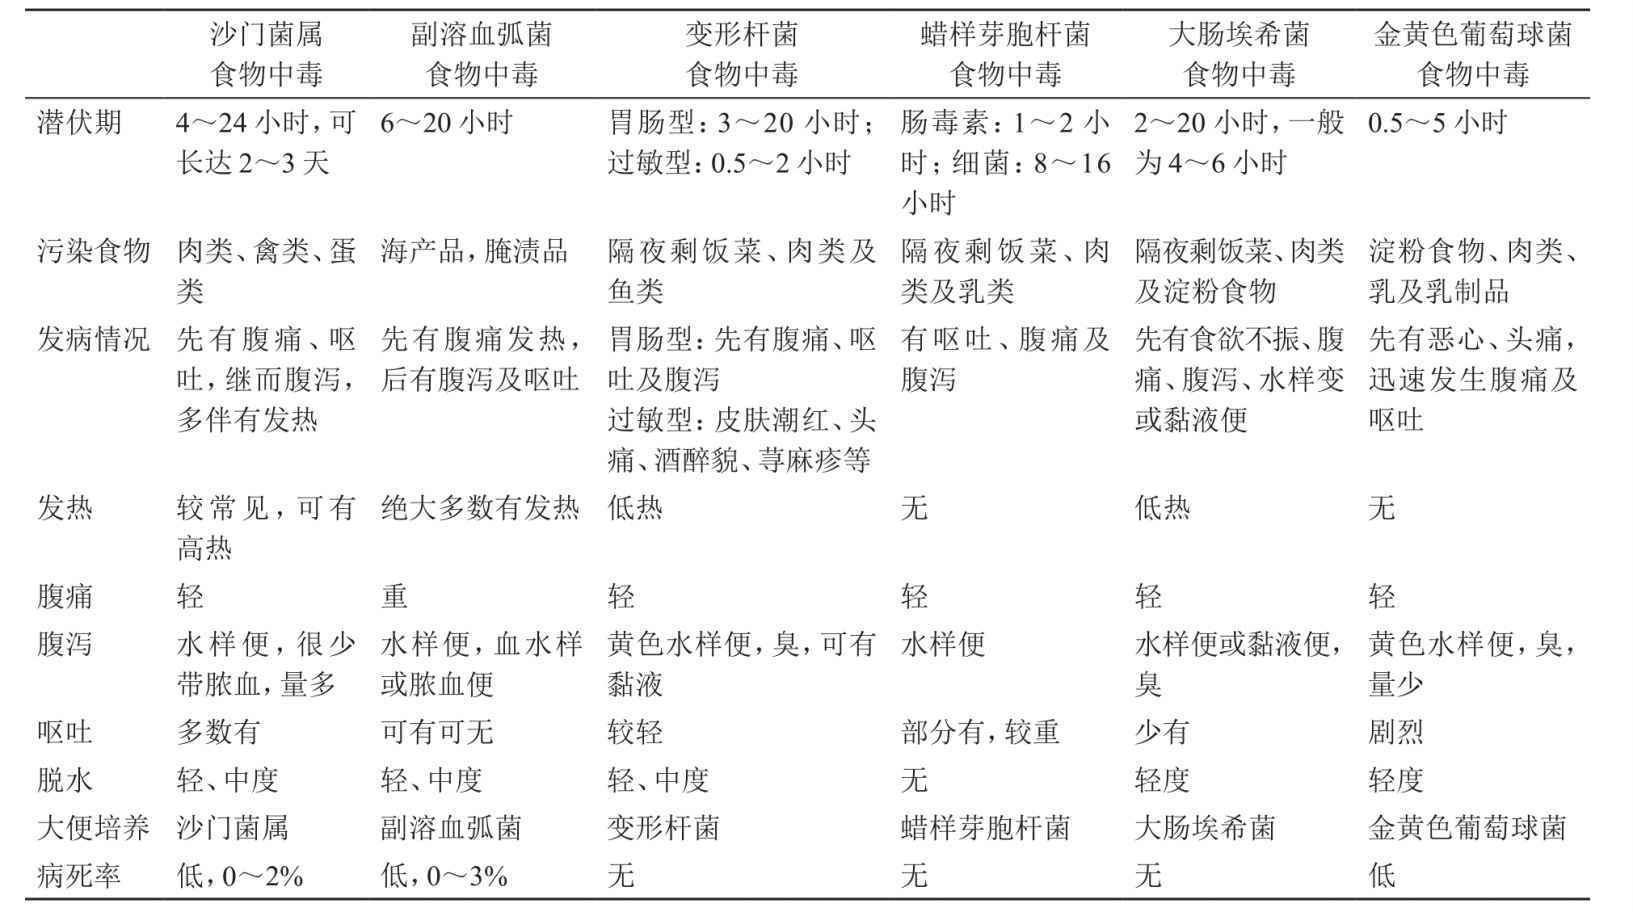
\includegraphics[width=6.72917in,height=3.75in]{./images/Image00236.jpg}
\end{table}

\paragraph{急性细菌性痢疾}

无明显进食污染食物和短时间内同食者集体发病史。发热,全身中毒症状较明显,腹泻以脓血便或黏液便为主,里急后重明显。大便培养有痢疾杆菌生长。

\paragraph{霍乱}

来自霍乱流行地区,有霍乱患者接触病史,常有先泻后吐,吐泻严重的特点。一般无腹痛,吐泻物呈米泔水样,脱水明显,可有肌痉挛。大便培养有霍乱弧菌。

\paragraph{急性出血性坏死性肠炎}

全身中毒症状重,可发生感染性休克。腹部有阵发性或持续性绞痛,并有明显压痛、反跳痛和肌紧张等腹膜刺激症状。大便可呈血水样,大便培养无致病菌生长。

\paragraph{病毒性胃肠炎}

无明显进食污染食物史,亦无短时间内集体发病史。大便多为稀便或水样便,大便培养无病原菌。

\subsection{治疗}

\subsubsection{对症支持疗法}

\paragraph{一般处理}

应适当休息,吐泻症状严重的患者应暂时禁食,待症状好转后,可给易消化的流质或半流质饮食。

\paragraph{对症处理}

①腹痛、呕吐症状严重者,可用山莨菪碱(654-2)10mg或罗痛定60mg肌肉注射,亦可口服丙胺太林15mg或颠茄片8mg或654-2片10mg,每日3次。②有发热及全身中毒症状者或有频繁呕吐及腹泻不能进食者,可静脉滴注5\%葡萄糖盐水、5\%~10\%葡萄糖液和林格液1000~2000ml/d。有高热及明显中毒症状者,可在静脉补液中加入氢化可的松100~300mg或地塞米松5~10mg,以降温和减轻中毒症状。③有脱水症状者可口服补液,不能口服者静脉补液,补液时先快后慢,补液量视脱水程度可达3000~6000ml/d。有酸中毒时适当补充5\%碳酸氢钠液或11.2\%乳酸钠溶液。补液患者出现排尿后,应及时补钾,以防出现低血钾表现。④过敏型变形杆菌食物中毒,可用抗组胺类药物,如氯苯那敏(扑尔敏)4~8mg或苯海拉明25mg,每日3次;亦可肌肉注射异丙嗪25~50mg。

\subsubsection{病原治疗}

症状轻者,一般不用抗生素。但有高热、中毒症状及吐泻严重者,可根据可能的病原菌,选用抗菌药物。可用氟喹诺酮类如诺氟沙星(氟哌酸,0.2g,每日3次)、环丙沙星(0.2~0.4g,每日3次)等口服,或氨基糖苷类如阿米卡星(丁胺卡那霉素,0.4g/d),庆大霉素(16万~24万U/d)、妥布霉素(16万~24万U/d)等加入液体中静滴或每日分2次肌肉注射。

\protect\hypertarget{text00184.html}{}{}

\section{神经型细菌性食物中毒}

神经型细菌性食物中毒,又称肉毒中毒(botulism),是由于进食含有肉毒梭状芽胞杆菌(简称肉毒杆菌)外毒素的食物而引起的中毒性疾病,临床上以神经系统症状如眼肌和舌咽肌麻痹为主要表现。如抢救不及时,病死率较高。

\subsection{病因与发病机制}

肉毒杆菌系严格厌氧的革兰阳性梭状芽胞杆菌。若细菌污染食物后,在缺氧情况下可以大量繁殖,并可产生外毒素。污染的食物主要为罐头食品、香肠、腊肉、发酵的豆制品(如臭豆腐、豆瓣酱、豆豉等)和发酵的面食(如发酵的馒头、面酱等)。肉毒杆菌外毒素依抗原性不同,可分为A、B、Ca、Cb、D、E、F、G等8型,引起人类疾病者主要是A、B和E型。肉毒杆菌外毒素是一种嗜神经毒素,毒力强大,对神经组织亲和力以A型为最强,E型次之,B型较弱。一般对人的致死量约为0.1~1μg。但此种毒素是一种对热不稳定的蛋白质,煮沸(100℃)10分钟或80℃经30分钟便可破坏,而胃酸和消化酶并不能破坏它,故人误食被污染而又未经煮沸的食品,便可发生严重的中毒。

肉毒杆菌外毒素经胃和小肠上段吸收,进入血液循环,主要作用于脑神经核、外周神经、神经肌肉接头处及自主神经末梢,抑制胆碱能神经传导介质乙酰胆碱的释放,使肌肉收缩运动障碍而发生瘫痪。

\subsection{诊断}

\subsubsection{临床表现特点}

潜伏期一般为12~36小时,可短至2小时,长达8~10天。潜伏期愈短,病情愈重。

临床症状轻重不一,轻型仅有轻微不适,重者可于24小时内死亡。一般起病急剧,以中枢神经症状为主,肠炎症状缺如或很轻微。初起时全身软弱、头痛、头晕,继而出现眼睑下垂、瞳孔扩大、复视、斜视及眼内外肌瘫痪;重症患者有吞咽、咀嚼、言语、呼吸等困难,声音嘶哑或失音,抬头困难、共济失调,但肢体完全瘫痪者少见。因胆碱能神经传递的阻断,可出现腹胀、尿潴留及唾液和泪液的减少等。体温多正常,患者神志清楚,感觉正常。脑脊液检查正常。死亡多是由于呼吸中枢麻痹、心力衰竭或继发肺炎所致,病死率因毒素类型而异,A型毒素者病死率为60\%~70\%,E型毒素者为30\%~60\%,B型毒素者为10\%~20\%。国内由于广泛采用多价抗毒素血清治疗本病,病死率已降至10\%以下。存活者于4~10天后逐渐恢复,呼吸、吞咽及言语困难先后缓解,随后其他肌肉瘫痪也渐复原。视觉恢复较慢,有时需数月之久。

\subsubsection{实验室检查}

\paragraph{细菌培养}

取污染食物作厌氧菌培养,可分离出肉毒杆菌。

\paragraph{动物中毒试验阳性}

(即用原可疑食品的浸出液注入小白鼠腹腔内或口饲,动物发生典型的瘫痪症状并迅速死亡)。

\subsubsection{诊断注意事项}

根据有进食可疑食物史,特别是变质的罐头、腊肉等腌制食品及发酵的豆、面制品等的病史,并且同食者先后发病,起病急骤,典型的脑神经麻痹症状如眼肌瘫痪、吞咽、发音及呼吸困难等即可作出临床诊断。此外,本病尚需与以下情况鉴别:

\paragraph{河豚或毒蕈中毒}

有误食河豚或毒蕈史可资鉴别。河豚或毒蕈中毒亦可出现神经麻痹症状,但主要为指端麻木及肢体瘫痪。肉毒中毒主要为脑神经麻痹,出现肢体瘫痪者少见。

\paragraph{脊髓灰质炎}

多见于小儿,有发热、肢体疼痛和肢体瘫痪。脑脊液检查有蛋白及白细胞数增多。

\paragraph{流行性乙型脑炎}

发病有明显季节性,在每年7~9月份,有发热、惊厥和昏迷,脑脊液蛋白和白细胞数增加。乙脑特异性IgM抗体阳性。

\paragraph{其他疾病}

如吉兰-巴雷综合征、重症肌无力等,参见有关章节。

\subsubsection{病情分级}

\paragraph{轻度}

仅有眼肌受累症状,如视力减退、视物不清,远视或近视,闭目无力,畏光,眼睑下垂、复视、斜视、瞳孔扩大及对光反应迟钝等。可伴有头痛、眩晕、全身乏力等一般症状。

\paragraph{中度}

除了眼肌受累外,口咽部肌肉受累,出现张口、咀嚼、吞咽困难,不能示齿、鼓腮,鼻唇沟变浅、构音障碍、言语不清、失声、咽干、咽喉部紧缩感、流涎等。

\paragraph{重度}

在以上症状基础上有呼吸肌受累表现,出现胸闷、憋气、发绀以至周围性呼吸衰竭,危及生命。

以上所有患者均可有骨骼肌不同程度的受累,当骨骼肌和呼吸肌完全受累者称为极重度。

\subsection{治疗}

\paragraph{洗胃导泻}

凡进食可疑食物24小时以内者,应尽早用1\%~2\%碳酸氢钠液或1∶4000高锰酸钾溶液反复洗胃。因碱性液可破坏肉毒杆菌外毒素,氧化剂不仅可减低外毒素毒力,并可抑制肉毒杆菌生长。洗胃后可注入药用炭30~50g吸附毒素同时用硫酸钠15~30g导泻,以排出毒素。

\paragraph{对症处理}

呼吸困难时吸氧,保持呼吸道通畅,必要时行气管插管或切开,人工呼吸。加强心电、血压、血氧饱和度监测。吞咽困难时鼻饲或静脉补充营养。有继发感染用抗生素治疗。

\paragraph{抗毒素治疗}

对本病有特效,使用越早,疗效越高,在发病后24小时内或发生肌肉瘫痪前治疗效果最佳。即使毒素已结合到神经肌肉接头上,抗毒素仍可起中和作用。对病菌型别未确定者,应注射多价抗毒素血清(A、B、E型),5万~10万U静脉及肌肉各半量注射,每12小时1次;对病菌型别已确定者,应注射同型单价抗毒素血清,每次1万U~2万U,每12小时1次。足疗程用药:轻度中毒一般连用3~5天;中度中毒一般连用5~7天;重度中毒一般连用7~10天以上。本品注射前须作皮肤过敏试验,阳性者需按脱敏方法进行注射。

\paragraph{抗菌治疗}

大剂量青霉素(800万U/d)治疗可减少肠道内肉毒杆菌菌量,防止外毒素继续产生和吸收。

\paragraph{神经肌肉营养药物的应用}

包括大剂量维生素C、ATP、CoA、胞磷胆碱等,以及维生素B\textsubscript{1}
100mg/d、维生素B\textsubscript{12} 0.5mg/d肌注。

\paragraph{其他治疗}

盐酸胍啶有促进周围神经释放乙酰胆碱作用,对神经瘫痪和呼吸功能有改进作用,剂量为每日15~50mg/kg,可经鼻饲给予。

\paragraph{保护易感人群}

若进食食物已证明有肉毒杆菌或其外毒素存在,或同进食者已发生肉毒中毒时,未发病者应立即注射多价抗毒素血清5000~10
000U,对病菌型别已确定者注射同型单价抗毒素血清1000~2000U,以防止发病。

\protect\hypertarget{text00185.html}{}{}

\hypertarget{text00185.htmlux5cux23CHP5-10-4}{}
参 考 文 献

1. 张文武.急诊内科手册.北京:人民卫生出版社,2009

2. 王洪林
.食用自制臭豆腐致肉毒梭状芽胞杆菌中毒17例报告.中华传染病杂志,1991,9:l59

3. 杨绍基,任红.传染病学.第7版.北京:人民卫生出版社,2008

4.
河北医科大学第二医院肉毒中毒救治专家组.肉毒中毒诊疗方案.中华急诊医学杂志,2010,19(4):349

5. 张文武.食物中毒的应急处理.中华急诊医学杂志,2008,17(8):895

\protect\hypertarget{text00186.html}{}{}

\chapter{日常生活用品中毒}

\section{洗涤剂中毒}

\subsection{中毒机制}

目前家用洗涤剂主要为两类:包括肥(香)皂、合成洗涤剂如洗衣粉等。现今的家用洗涤剂主要成分毒性很低。皂类:主要成分为硬脂酸钠,碱性强,无显著刺激性,广泛应用于洗衣、沐浴、清洁环境,通过往皂基中加入各种添加剂制成香皂、药皂等多种种类。肥皂呈碱性,对皮肤黏膜有一定的刺激性。长时间、高浓度接触可造成接触部位的损害。洗衣剂分为粉状的洗衣粉和液状的洗衣水。主要成分是多种阴离子表面活性剂(如烷基苯磺酸钠、烷基磺酸钠、脂肪醇、硫酸钠、脂肪醇聚氧乙烯醚硫酸钠等)以及非离子表面活性剂(如环氧乙烷、环氧丙烷的共聚物)。此外,还含有一些无机盐助剂(主要是三聚磷酸钠)和有机助剂(主要是羧甲基纤维素)。洗衣剂所含有的成分多为低毒或无毒物质。一般皮肤接触对人体无明显的毒作用。酶添加剂可引起敏感个体的哮喘和皮肤过敏。洗衣粉对人体健康影响主要是表面活性剂对蛋白质的结合,并促使其溶解。误服后表现为胸骨后、上腹部灼痛,恶心、呕吐、腹泻等症状。洗涤剂一般毒性较低,但是由于部分添加杀菌剂或消毒剂,对皮肤刺激较大,部分含有氨水,有轻微刺激气味,由于洁厕净成分中含有腐蚀性的稀盐酸,为含酸腐蚀性洗涤剂,人体食入后能很快腐蚀食管、消化道等器官,如护理不周,极易引起各种并发症。

\subsection{诊断}

\paragraph{病史}

包括皮肤接触,误食、误用洗涤剂史。

\paragraph{临床表现特点}

洗衣粉及洗涤剂毒性低,一般无明显皮肤刺激作用,误服一般不会出现严重损伤,主要表现为胸骨后、上腹部烧灼感,可出现恶心、呕吐、腹泻等症状,以吐泻物带有大量泡沫为特征,偶有严重者可有呕血、黑便、低血压、食管或胃穿孔甚至发生休克。由于洁厕净剂部分产品含30\%盐酸,吞食酸性腐蚀性洁厕类物质,可引起表层组织脱水,蛋白变性、凝固、坏死,形成焦痂。焦痂常在3~4天脱落,出现出血;焦痂脱落后第3~4天可出现穿孔。吞食后胸骨后和腹部剧烈疼痛、烧灼感;部分患者有食管损伤、胃损伤甚至出现小肠损伤,可有腹痛、恶心、呕吐、呕血等症状。呼吸道刺激引发咳嗽、声嘶、喘息甚至出现喉头水肿、喉痉挛、肺水肿。严重时可出现因穿孔出血伴发休克。部分中毒者出现低钙、低镁、高血钾、低血压、休克、心律失常、抽搐及心跳停止。

\subsection{治疗}

\paragraph{皮肤刺激}

用大量清水进行清洗,溅入眼内立即用大量清水冲洗。

\paragraph{口服中毒}

①保护胃黏膜:洗衣粉毒性低,无特殊解毒剂,可按上消化道碱灼伤处理,可立即饮用食醋中和并服用少量蛋清、牛奶或植物油保护胃肠黏膜。由于洁厕净腐蚀性较强,口服洁厕净后很快腐蚀消化道致黏膜烧伤、腐蚀出血,甚至穿孔;同时伴有机体酸碱失衡,一般不适宜洗胃治疗,因为洗胃会增加毒物在体内的停留和吸收,所以提倡尽早采用生鸡蛋清、氢氧化铝、果胶铋等口服,以保护胃黏膜,并尽早应用护胃制酸剂,隔离毒物以延缓和减少毒物吸收。但口服量较大者,可插鼻胃管引流出胃内容物,对治疗有好处,根据情况考虑是否洗胃。不主张用中和剂,以防产热过量诱发呕吐。禁食并给予H\textsubscript{2}
受体阻滞剂减少胃酸分泌,双八面体蒙脱石(思密达)对消化道黏膜有很强的覆盖保护能力,修复、提高黏膜屏障对攻击因子的防御功能,保护黏膜,减少出血。②防止继发呼吸道感染:应尽可能安置在监护室,保持空气洁净度。同时严密观察病情,做好呼吸道管理,监测动脉血气分析,防治ARDS发生。除配合早期综合治疗措施外,关键是加强呼吸道和消化道的管理,并密切观察病情变化,及时对症处理,防治并发症的发生。③心肝肾功能监测:密切监测心、肝、肾功能情况,预防并发症发生,定期检查血、尿、大便常规、大便潜血及肝肾功能生化指标,发现异常情况及时处理。④对症治疗:严重者酌情止痛、防治休克,及时对症处理。

\subsection{预防}

为防止洗涤剂引起中毒,在选购洗涤剂时应注意其成分说明,注意阅读注意事项及产品说明,避免将不同成分洗涤剂、消毒剂混合使用,在使用过程中注意开启门窗,充分通风,避免气体浓度过高,将洗涤剂放置于阴凉、干燥、通风处及儿童不易接触的地方。应避免使用酒瓶、饮料瓶盛装,以免误服、误用。

\protect\hypertarget{text00187.html}{}{}

\section{洁厕剂中毒}

洁厕剂产品有便池清洁剂、洁厕灵、去油净等。一般为浅蓝色酸性透明或无色液体,主要成分为酸类、表面活性剂和消毒剂。如:烷基苯磺酸、壬基酚聚氧乙烯醚、硫酸氢钠、氨基磺酸、草酸、去离子水等。此类产品成分差别很大,少数产品含有强酸,具有腐蚀性。所以使用时要严格按照说明书上的使用范围及使用方法应用。

\subsection{中毒机制}

本品对眼和皮肤黏膜有腐蚀作用。吞食酸性腐蚀性洁厕类物质,可引起表层组织脱水,蛋白变性、凝固、坏死,形成结痂。咽部和食道的鳞状上皮对酸类腐蚀物有一定的抵抗,吞食后6\%~20\%的患者有食道损伤。20\%的患者出现小肠损伤。焦痂常在3~4天脱落,出现出血,焦痂脱落后第3~4天可出现穿孔。口服可引起口腔黏膜、消化道、胃黏膜损伤。严重者可造成消化道出血、穿孔。

\subsection{诊断}

皮肤接触一定时间后出现剧痛,接触部位呈淡黄色。眼睛溅入后可产生结膜水肿与角膜损伤、疼痛、流泪及畏光。中毒患者出现呼吸困难,呼吸窘迫、喘息、吞咽困难、口痛、胸痛、腹痛、恶心、呕吐、气道梗阻、声嘶、喘鸣、发音困难、失声、心动过速、流口水、皮下气肿、急性腹膜炎、呕血。重症患者胸骨后和腹部剧烈疼痛、烧灼感、黏膜糜烂、坏死,严重者穿孔、出血伴发休克、喉头水肿、喉痉挛。部分中毒者出现低钙、低镁、高血钾、低血压、休克、心律失常、抽搐及心跳停止。

\subsection{治疗}

皮肤接触者要立即用清水冲洗皮肤至少15分钟。衣服污染时要立即脱去衣服,并直接用水冲洗污染的部位。溅入眼睛者要及时用流动水冲洗至少15分钟。冲洗时须将眼睑分开。口服者若在10分钟内,可一次口服清水1000ml或大量饮用牛奶,但如口服时间已超过10分钟,不可饮用任何液体。对于腐蚀类化学用品中毒,是否洗胃观点不一致。口服量较大者,可插鼻胃管引流出胃内容物,对治疗有好处,应根据情况考虑是否洗胃。不主张使用中和剂,以防产热过量诱发呕吐。应禁食,给予H\textsubscript{2}
受体阻滞剂减少胃酸分泌,蒙脱石散对消化黏膜有很强的覆盖保护能力,修复、提高黏膜屏障对攻击因子的防御作用,保护黏膜,减少出血。根据患者情况可给予对症支持治疗。

\subsection{预防}

妥善保存,正确使用,避免溅到皮肤和眼内。

\protect\hypertarget{text00188.html}{}{}

\section{消毒剂中毒}

消毒剂是指可在体外迅速杀灭病原微生物和其他有害微生物,以切断致病传播途径,从而达到预防和控制感染性疾病目的的制剂。近年来由于人们对环境卫生的重视,消毒剂得到了广泛的运用,但是由于不注意消毒剂的安全使用或误服引起中毒,可对人体健康造成损害,甚至可以引起死亡。

\subsection{分类}

\paragraph{按照其作用水平}

可分为:①灭菌剂:可杀灭一切微生物而达到无菌作用。包括甲醛、戊二醛、环氧乙烷、过氧乙酸、过氧化氢、二氧化氯等;②高效消毒剂:可杀灭细菌繁殖体(包括分枝杆菌)、病毒、真菌及其孢子等,对细菌芽胞也有一定杀灭作用,包括含氯消毒剂、臭氧、甲基乙内酰脲类化合物、双链季铵盐等;③中效消毒剂:仅可杀灭分枝杆菌、真菌、病毒及细菌繁殖体等微生物,包括含碘消毒剂、醇类消毒剂、酚类消毒剂等;④低效消毒剂:只可杀灭细菌繁殖体和亲脂病毒,包括季铵盐类消毒剂、双胍类消毒剂、金属离子类消毒剂及中草药消毒剂。

\paragraph{按化学性质的不同}

现在较常用的化学消毒剂包括:①过氧化物类消毒剂:包括过氧化氢、过氧乙酸、二氧化氯和臭氧等;②含氯消毒剂:包括:无机氯化合物,如次氯酸钠、漂白粉等;有机氯化合物,如二氯异氰尿酸钠、三氯异氰尿酸等;③醛类消毒剂:包括甲醛和戊二醛;④醇类消毒剂:最常用的是乙醇、异丙醇及复合醇消毒剂,这些产品多用于手部皮肤消毒;⑤含碘消毒剂:包括碘酊和聚维酮碘;⑥酚类消毒剂:包括苯酚、甲酚、卤代苯酚及酚的衍生物;⑦双胍类和季铵盐类消毒剂:它们属于阳离子表面活性剂,具有杀菌和去污作用;⑧季铵盐类消毒剂:包括苯扎溴铵、氯己定、消毒灵等。⑨杂环类消毒剂,如环氧乙烷;⑩重金属类消毒剂,包括硝酸银和汞化合物等。

\subsection{中毒机制}

常用的消毒剂多为低毒或中等毒类,多数消毒剂是稀释后使用,因此毒性一般不大。大多数消毒剂对皮肤黏膜都有明显的刺激作用,苯酚、甲醛、高锰酸钾等腐蚀作用较强,呼吸道吸入后,可致吸入性肺炎、化学性肺炎甚至化学性肺水肿。环氧乙烷对中枢神经有抑制作用。强氧化性消毒剂如二氧化氯、氯胺、次氯酸钠以及重金属类消毒剂如硝酸银等还可致高铁血红蛋白血症。少数消毒剂如氯胺、二氧化氯、过氧乙酸、甲酚皂(来苏尔)可以发生溶血。过氧化物类消毒剂及含氯消毒剂因其氧化能力强,高浓度时可刺激、损害皮肤黏膜致使黏膜、气道、肺泡上皮细胞和毛细血管内皮细胞膜蛋白破坏,最终可引起低氧血症、呼吸窘迫。含氯消毒遇酸后可产生氯气,吸入后出现明显呼吸道刺激症状。环氧乙烷、酚类、醛类消毒剂可引起心肌损伤,出现心动过缓以及期前收缩等心律失常。臭氧、醇类消毒剂可以使周围血管扩张,引起血压下降。汞化合物进入人体后,与酶蛋白的巯基结合,抑制了多种酶的活性,使组织细胞的正常代谢发生障碍。

\subsection{诊断}

\subsubsection{病史}

有消毒剂接触史或误服史。

\subsubsection{临床表现特点}

\paragraph{过氧化物类消毒剂}

包括二氧化氯、过氧化氢,两者均为低毒。3\%的过氧化氢未发现明显的皮肤、眼、黏膜毒性作用;口服大量的3\%过氧化氢会发生呕吐、腹痛和腹泻。过氧乙酸为中等毒,对皮肤黏膜有刺激作用。皮肤接触高浓度溶液可出现局部水疱、红肿、皮炎、溃疡等;溅入眼睛后可出现疼痛、畏光、流泪等刺激症状,严重者出现角膜水肿、溃疡穿孔甚至失明。口服高浓度溶液后口腔、咽喉、食管和胃有烧灼感,出现消化道溃疡、出血甚至穿孔,严重者可昏迷、抽搐、休克。吸入高浓度蒸气可引起严重的呼吸道刺激症状,出现咳嗽、气喘、呼吸困难,甚至化学性肺水肿。臭氧为低毒,吸入臭氧后,对眼睛有刺激,出现疼痛、畏光、流泪等症状,呼吸系统可出现咽喉干燥、咳嗽、咳痰、胸闷等,重者出现肺水肿。

\paragraph{含氯消毒剂}

属低毒,主要表现为:①皮肤黏膜刺激作用:其粉尘对眼和上呼吸道有刺激作用。其水溶液溅入眼睛,可出现疼痛、畏光、流泪等刺激症状。皮肤接触高浓度水溶液可出现局部水疱、红肿、皮炎等。②呼吸道刺激作用:本类消毒剂遇酸后可产生氯气,吸入后出现明显呼吸道刺激症状,如咳嗽、气喘、呼吸困难等,严重者出现化学性支气管炎、肺炎,甚至肺水肿。③消化道刺激作用:误服少量时无明显症状,大量口服后口腔、咽喉、食管和胃有烧灼感,出现恶心、呕吐、呕血,甚至出现胃穿孔和腹膜炎,严重者可导致循环衰竭。

\paragraph{醛类消毒剂}

包括甲醛和戊二醛,为中等毒,对皮肤黏膜有刺激腐蚀作用,少数人出现过敏性皮炎,表现为粟粒至米粒大小红色丘疹,周围皮肤潮红或轻度红肿,皱裂部位可见湿润现象,瘙痒明显。眼睛接触后出现视物模糊、畏光、流泪、疼痛。短期内接触高浓度蒸气,引起以呼吸系统损害为主的全身性症状,轻度中毒有头晕、头痛、乏力等症状,重度中毒时可因喉头水肿、肺水肿、昏迷、休克致死;口服后因消化道腐蚀性损伤出现上腹剧痛,有血性呕吐物,胃肠道糜烂、溃疡、穿孔,可引起多脏器损害而死亡。

\paragraph{醇类消毒剂}

属微毒类,但大剂量对中枢神经系统有麻醉作用,其蒸气对眼及呼吸道黏膜有刺激作用。大剂量服用后出现流涎、恶心、呕吐、腹痛、头痛、眩晕、共济失调,重者可发生出血性胃肠炎、肺水肿、脑水肿、肾功能衰竭等,甚至昏迷、死亡;少数病例可出现接触性皮炎。

\paragraph{含碘消毒剂}

属低毒,稀溶液毒性低,无腐蚀性。皮肤接触高浓度聚维酮碘,可变为棕黄色、可引起灼伤、坏死,少数人有皮肤过敏反应。吸入碘蒸气,可发生严重的刺激症状,如结膜炎、流涕、咽发干并有烧灼感及异物感,黏膜上有褐色痂皮,咳嗽,呼吸困难,口腔黏膜及声门水肿,发生喉头水肿时,可致窒息甚至导致肺炎及肺水肿。此外,尚可发生视觉障碍、耳鸣、头痛、嗜睡等。口服过量可发生腐蚀性胃肠炎,出现呕吐、呕血、烧灼感、便血、休克等症状,呕吐物为黄色,如胃中有淀粉存在,则变为蓝色,粪内有血。严重病例有四肢震颤、发绀、惊厥、休克及昏迷等,或有出血性肾炎。

\paragraph{酚类消毒剂}

属中等毒,皮肤接触可引起局部灼伤和皮炎;溅入眼内引起角膜、结膜灼伤;误服引起消化道灼伤,有呕吐、便血、胃肠穿孔,并可引起肺水肿和肝、肾、胰等多脏器损害;部分病例对甲酚有哮喘和皮肤过敏反应。

\paragraph{双胍类消毒剂}

属低毒,无刺激性,大量口服时可有胃肠道刺激症状,如恶心、呕吐、腹泻等。

\paragraph{季铵盐类消毒剂}

毒性低,刺激性小。1∶1000的溶液用于皮肤、环境、金属器械及橡胶制品消毒。口服大量高浓度溶液时出现胃肠道刺激症状,如恶心、呕吐、烦躁不安、肌无力、昏迷、痉挛,严重者可因呼吸麻痹而致死;偶见过敏反应。

\paragraph{杂环类消毒剂}

常用的是环氧乙烷,中等毒,低浓度时有刺激作用,高浓度则对中枢神经有抑制作用。环氧乙烷蒸气对皮肤一般不产生刺激,因环氧乙烷极易溶于水,若接触部位沾水或出汗,便可发生严重皮炎。液体沾染皮肤时,由于蒸发可引起冻伤或灼伤,愈后可留有黑棕色色素沉着,皮肤反复接触时可有过敏反应。接触大量环氧乙烷气体后呼出气有特殊的甜味,迅速出现眼、鼻、咽喉、支气管刺激症状,并有剧烈头痛、嗅味觉消失、恶心、频繁呕吐、四肢无力、共济失调、发绀、呼吸困难;严重者出现肺水肿,甚至昏迷、死亡。

\paragraph{重金属类消毒剂}

中等毒性,接触浓缩的硝酸银,皮肤、黏膜可出现溃疡及变色。口服硝酸银,可出现口腔黏膜呈白色,有腐蚀性溃疡,口、咽及上腹部烧灼感,剧烈腹痛、流涎、恶心、呕吐、吐出物为白色或棕色,暴露后呈黑色,偶有腹泻;并可出现眩晕、惊厥、昏迷、麻痹、呼吸困难和休克,亦可发生窒息及肺水肿。长期接触银盐,可使皮肤发生蓝黑色的色素沉着,称为银质沉着症。齿龈及指甲亦可变色。有高铁血红蛋白血症时,皮肤出现青紫色。汞化合物中毒时可出现明显的口腔黏膜肿胀、充血或溃疡出现,口内有金属味,流涎增多。消化系统症状为恶心、呕吐、食欲不振、腹痛、腹泻、黏液便或血便等症状。神经系统症状:患者倦怠、嗜睡、头痛、头晕、心悸、全身极度衰弱。重者有痉挛,以至昏迷。泌尿系统症状:尿少,蛋白尿,尿中有红细胞和管型等,严重者可发生急性肾功能衰竭。由于肾小管坏死可致汞毒性肾病。此外,尚可有发热、咳嗽等类似肺炎的表现。并可有肝脏肿大及皮炎。

\subsection{治疗}

各类消毒剂中毒均无特效解毒剂,发生中毒后应将中毒患者立即移离现场,脱去污染衣物,注意休息、保暖,加强监护。

1.皮肤接触有较强腐蚀性的消毒剂后,立即用大量清水反复冲洗,如环氧乙烷液体沾染皮肤,可使用3\%硼酸溶液反复冲洗;甲酚皂污染皮肤后用清水反复冲洗干净,再使用硫酸钠饱和溶液湿敷4~6小时。出现红肿、水疱并伴有糜烂渗出者应按皮肤科常规处理。

2.溅入眼睛者
,立即以大量流动清水冲洗15分钟,眼内涂抹四环素可的松眼膏、红霉素眼药膏或氯霉素眼药水,如果症状持续加重,立即请眼科医师会诊。

3.吸入中毒后
,迅速将中毒者移至通风处,保持呼吸道通畅,如出现咳嗽、呼吸困难等呼吸道刺激症状,及时给予呼吸道解痉剂、镇咳剂和镇静剂;对于因喉头水肿、痉挛、呼吸道灼伤分泌物多而致呼吸困难或窒息者,应及时做气管切开,积极防治呼吸道感染,出现肺损伤,应早期足量应用糖皮质激素,必要时使用呼吸机治疗,积极防治肺水肿和呼吸道感染,保护各脏器功能。

4.口服中毒后,立即给予口服100~200ml的牛奶、生蛋清或氢氧化铝凝胶保护消化道黏膜。一般情况下不主张洗胃、催吐、导泻及使用酸碱中和剂。如果服用了大量高浓度腐蚀性强的消毒剂,应早期细心下胃管并予以保留,避免因操作不当引起消化道穿孔,然后小心使用牛奶或氢氧化铝凝胶洗胃,可较好地减轻消毒剂对消化道黏膜损害作用,每次灌入量小于100ml,最后保留胃管,防止食管狭窄。甲酚皂中毒后立即口服植物油30~60ml,然后口服牛奶或氢氧化铝凝胶;口服含碘消毒剂后应服用大量淀粉、米汤;甲醛中毒后服用3\%碳酸铵或15\%乙酸铵(醋酸铵)100ml,使甲醛变为毒性较小的六亚甲基四胺。可静注高渗葡萄糖液,促进毒物由尿排泄。如有脱水、酸中毒和电解质失衡时,可根据具体情况补充液体。

5.解毒剂
消毒剂中毒多无特效解毒剂,重金属类消毒剂中毒的解毒剂如巯基化合物:二巯丙醇、二巯基丙磺酸钠或二巯基丁二酸钠应尽早使用,若出现明显的肾功能损害时,则疗效欠佳。在无上述解毒剂时也可用青霉胺治疗。此药有类似二巯丙醇的作用,其疗效虽不及上述解毒剂,但可口服,毒性很小。

6.对症治疗
保护脏器功能。消毒剂中毒后可引起多脏器损害,应密切观察各脏器的功能变化,纠正水、电解质紊乱及酸碱失衡,保护内环境稳定,改善各脏器功能,防止发生循环衰竭和肾功能衰竭。发生过敏反应时给抗过敏药物。醇类消毒剂重度中毒时使用血液透析。

\subsection{预防}

使用消毒剂进行消毒处理时,应穿戴防护用具(口罩、手套、防护服、眼罩等),按规定浓度配制和使用消毒液,仔细阅读产品说明书,按说明提示使用,禁止多种洗涤剂同时混用,使用过程中注意开启门窗,保持空气流通。在进行熏蒸消毒时,人员不要在消毒地点停留,消毒完毕后,通风1~2小时再进入消毒地点。处理消毒剂泄漏时,必须戴好防毒面具与手套,使用大量清水冲洗干净,经稀释的污水排入废水系统。应保存在密闭容器内,放在凉爽、干燥、通风处,注明成分,防止误服。家庭使用的消毒剂应当保存在小儿不易接触到的地方。避免使用酒瓶、饮料瓶盛装消毒剂,以免误服、误用。

\protect\hypertarget{text00189.html}{}{}

\section{化妆品中毒}

现在各年龄阶段都有适用的化妆品,化妆品深刻的影响着我们的生活。化妆品都是化学合成品,虽然有美化功能,但是也存在着有害作用。在化妆品中,由于需要增加祛斑美白的功效添加了汞、砷、铅等化学成分,容易引起人体中毒。

\subsection{分类与中毒机制}

化妆品分为护肤品(包括清洁剂),美容品,美发用品和香料四大类。护肤品亦成为基础化妆品,其作用是清洁皮肤、保持油脂分泌和水分发挥的平衡,促进新陈代谢及保护皮肤免受有害紫外线的影响。其包括了日常使用的洁面用品、膏霜、乳液、化妆水、凝胶制品、面膜等。

美容化妆品用以涂覆于脸部及指甲等部位而赋予色彩,改变肤色、形成层次,以增强美感。包括了粉底、唇膏、胭脂、眉目用品、指甲用品及香粉等。

美发化妆品是洁发、清洁头发、卷发及营养效用的化妆品。包括护发素、染发剂、卷发剂和定型剂等。

芳香化妆品以赋香为主要目的,包括香水、花露水等。

化妆品的原料有香料、防腐剂、抗氧化剂、色素、基质、金属皂、非甘油酯等,在绝大部分情况下,不会产生不良反应。但是在皮肤破损,或者是超敏体质下,可引起皮肤过敏反应。化妆品所致不良反应有:①刺激性反应:一般较轻、持续时间较短,仅有暂时性烧灼感、刺痒感。②接触性皮炎:有人对松香、对苯二胺、季铵盐及羊毛醇斑贴试验阳性,在使用含有上述物质的化妆品后即可出现接触性皮炎,表现为皮肤发红,红疹,甚至水肿。③光敏性皮炎:有些指甲油抛光剂中含有荧光剂等,在日晒后可出现指甲剥离。④接触性荨麻疹:某些化妆品可引起荨麻疹。⑤痤疮:有些化妆品可加重原先存在的痤疮。⑥色素改变:有些化妆品因原料中使用氢醌类物质而致接触性皮炎,消退后可出现色素沉着。⑦染发剂所致高铁血红蛋白血症:有的永久性染发剂中含苯的氨基及硝基化合物,如短期内大量接触,可出现高铁血红蛋白血症。

\subsection{常见化妆品中毒与处理}

\subsubsection{冷霜中毒}

该类化妆品包括香脂、雪花膏、润肤霜等。其主要原料有白蜂蜡、表面活性剂、硼砂和液状石蜡等,多加有香料。①病因及中毒机制:某些冷霜中的溴酸盐、硼砂有一定的毒性。硼砂属低毒类。溴酸盐对皮肤有一定的刺激性。②临床表现:不含溴酸盐、硼砂的润肤品误食后一般不会发生急性中毒症状。若摄入含有溴酸盐、硼砂的化妆品后,可出现呕吐,腹泻,腹痛,少尿或无尿,嗜睡,昏迷等表现。③治疗:误食不含溴酸盐、硼砂的冷霜类化妆品无需处理。若摄入含有溴酸盐、硼砂的化妆品,应口服催吐药物或人工催吐,催吐后口服牛奶。出现中毒表现者到医院治疗。④预防:选购不含有害物质的润肤品,存放在小儿不易接触到的地方。

\subsubsection{染发剂中毒}

染发剂主要分为两类:一类为通过对头发的色素氧化,改变头发的颜色。这类染发剂的主要成分是氧化剂(6\%的过氧化氢)和苯的胺基和硝基化合物类(萘胺、间苯二酚和甲苯胺等),产生永久性染发效果。另一类主要成分为丙二醇、异丙醇(两者约占50\%)、酚类化合物(低于1\%)以及其他添加剂,有的配方中还含有铅、银、汞、砷和铋(含量均低于0.1\%)。这类染发剂染上的颜色随着时间会逐渐脱失。①病因及中毒机制:有毒成分在两类染发剂中的浓度均较低,误食后一般不会发生严重的中毒情况。但大量摄入后,根据所含的有毒物种类可出现相应的中毒表现。过氧化氢对消化道黏膜有一定刺激性作用。②临床表现:少量摄入可出现消化道刺激症状,多表现恶心、腹部不适。大量摄入后可出现无力、头痛,恶心、呕吐、腹痛、发绀、眩晕等,严重中毒者可出现溶血、血压下降、嗜睡及昏迷。苯胺类尚可引起皮肤刺激症状。③治疗:皮肤污染要及时用清水冲洗。误食者要及时口服催吐药物或手法催吐,催吐后给患者活性炭。出现中毒表现者要及时到医院就诊。

\subsubsection{护发素中毒}

护发素主要成分为十八烷基三甲基氯化铵、双十八烷基二甲基氯化铵、十八烷基二甲基苄基氯化铵和十二烷基三甲基氯化铵等阳离子表面活性剂,还有一些添加剂(醇类、色素、pH调整剂、香料)和水。①病因及中毒机制:护发素中阳离子活性剂的浓度约为0.5\%~1.5\%。阳离子活性剂的浓度超过0.5\%时对黏膜即有明显的刺激作用,10\%时对食管和黏膜有腐蚀作用,20\%时能导致消化道穿孔和腹膜炎。口服吸收后可引起中枢神经症状。②临床表现:误服可出现呕吐,四肢乏力,严重者可昏迷。对口腔、食管及消化道黏膜有腐蚀作用。③治疗:皮肤、黏膜沾染了高浓度的护发素后要彻底清洗,可先用肥皂水清洗,再用清水冲去残留的肥皂。误服者可服活性炭或牛奶,出现中毒症状者要到医院予以对症处理。④预防:护发素使用后要冲洗干净,避免高浓度护发素溅入眼内。存放在儿童不易接触到的地方。

\subsubsection{洗发香波中毒}

洗发香波也称洗头水。可呈水状、糊状或膏状。主要成分为阴离子表面活性剂,如脂肪醇硫酸钠、脂肪醇聚乙烯醚硫酸钠、烯基磺酸钠、烷基硫酸胺等,还含有咪唑啉、甜菜碱等两性表面活性剂。现使用的香波一般不含烷基苯磺酸钠。但多添加有香精、色素。①病因及中毒机制:所含成分多为低毒或无毒物质,一般剂量对人体无明显的毒作用,高浓度对皮肤黏膜有一定的刺激性。敏感个体可出现哮喘和皮肤过敏。②中毒表现:眼睛接触高浓度香波液可产生刺激作用。误食大量洗发剂后可出现恶心、呕吐、腹痛、腹泻等症状。部分接触者可引起皮肤过敏或哮喘。③治疗:进入眼睛后,立即用清水冲洗干净。误服者可给服牛奶或温开水,无需催吐。④预防:避免高浓度香波溅入眼内。使用香波后,用清水将皮肤冲洗干净,过敏者可更换香波种类。

\subsubsection{烫发剂中毒}

烫发剂主要成分为巯基醋酸盐、胺类化合物、烷基聚氧乙烯醚,此外还有一些其他添加剂(如香精等)。①致病机制:对皮肤黏膜有刺激性,进入人体内可造成神经系统、消化系统功能紊乱。②临床表现:局部皮肤接触后可引起刺激性反应及过敏性皮炎,表现水肿、皮疹、皮肤灼感及瘙痒感。误食后可引起消化道刺激症状,表现为恶心,呕吐,腹泻和腹痛。吸收后可导致低血糖、中枢神经系统抑制、惊厥、呼吸困难等。③治疗:皮肤接触者可用大量清水冲洗。口服者要及时服催吐剂或采用手法催吐。出现低血糖,中枢神经系统抑制等临床表现后,给予对症支持治疗,无特效解毒剂。④预防:妥善保管,存放在小儿不易接触到的地方。

\subsubsection{脱毛剂中毒}

脱毛剂主要成分为硫化钡、碱类,其他添加剂含量均较低。含有的少量钡离子进入机体后,对骨骼肌、平滑肌、心肌等各类肌肉组织产生过度的刺激和兴奋作用。引起心脏传导阻滞等改变。但因脱毛剂中可溶性钡盐和碱类的含量较低,少量脱毛剂一般不会出现严重中毒。大量摄入后主要表现为恶心、呕吐、腹痛、腹泻等消化道刺激症状。脱毛剂种类和进食量的不同,临床表现可有较大的差别。部分患者皮肤接触后可发生皮肤灼伤或过敏反应。误服者要立即口服催吐药物或手法催吐,催吐后给予牛奶或活性炭。发生过敏反应时立即停用脱毛剂。出现中毒表现者予以对症治疗。预防:不要使用无正规生产厂家和批准号的产品,严格按照使用说明书使用。脱毛剂要存放在小儿不易接触到的地方。

\protect\hypertarget{text00190.html}{}{}

